% Generated by Sphinx.
\def\sphinxdocclass{report}
\documentclass[letterpaper,10pt,english]{sphinxmanual}
\usepackage[utf8]{inputenc}
\DeclareUnicodeCharacter{00A0}{\nobreakspace}
\usepackage{cmap}
\usepackage[T1]{fontenc}
\usepackage{babel}
\usepackage{times}
\usepackage[Bjarne]{fncychap}
\usepackage{longtable}
\usepackage{sphinx}
\usepackage{multirow}


\title{Java krok po kroku Documentation}
\date{November 30, 2014}
\release{0.1}
\author{Slawomir Ludwiczak}
\newcommand{\sphinxlogo}{}
\renewcommand{\releasename}{Release}
\makeindex

\makeatletter
\def\PYG@reset{\let\PYG@it=\relax \let\PYG@bf=\relax%
    \let\PYG@ul=\relax \let\PYG@tc=\relax%
    \let\PYG@bc=\relax \let\PYG@ff=\relax}
\def\PYG@tok#1{\csname PYG@tok@#1\endcsname}
\def\PYG@toks#1+{\ifx\relax#1\empty\else%
    \PYG@tok{#1}\expandafter\PYG@toks\fi}
\def\PYG@do#1{\PYG@bc{\PYG@tc{\PYG@ul{%
    \PYG@it{\PYG@bf{\PYG@ff{#1}}}}}}}
\def\PYG#1#2{\PYG@reset\PYG@toks#1+\relax+\PYG@do{#2}}

\expandafter\def\csname PYG@tok@na\endcsname{\def\PYG@tc##1{\textcolor[rgb]{0.25,0.44,0.63}{##1}}}
\expandafter\def\csname PYG@tok@gs\endcsname{\let\PYG@bf=\textbf}
\expandafter\def\csname PYG@tok@nf\endcsname{\def\PYG@tc##1{\textcolor[rgb]{0.02,0.16,0.49}{##1}}}
\expandafter\def\csname PYG@tok@no\endcsname{\def\PYG@tc##1{\textcolor[rgb]{0.38,0.68,0.84}{##1}}}
\expandafter\def\csname PYG@tok@sr\endcsname{\def\PYG@tc##1{\textcolor[rgb]{0.14,0.33,0.53}{##1}}}
\expandafter\def\csname PYG@tok@c1\endcsname{\let\PYG@it=\textit\def\PYG@tc##1{\textcolor[rgb]{0.25,0.50,0.56}{##1}}}
\expandafter\def\csname PYG@tok@o\endcsname{\def\PYG@tc##1{\textcolor[rgb]{0.40,0.40,0.40}{##1}}}
\expandafter\def\csname PYG@tok@k\endcsname{\let\PYG@bf=\textbf\def\PYG@tc##1{\textcolor[rgb]{0.00,0.44,0.13}{##1}}}
\expandafter\def\csname PYG@tok@ne\endcsname{\def\PYG@tc##1{\textcolor[rgb]{0.00,0.44,0.13}{##1}}}
\expandafter\def\csname PYG@tok@gp\endcsname{\let\PYG@bf=\textbf\def\PYG@tc##1{\textcolor[rgb]{0.78,0.36,0.04}{##1}}}
\expandafter\def\csname PYG@tok@ss\endcsname{\def\PYG@tc##1{\textcolor[rgb]{0.32,0.47,0.09}{##1}}}
\expandafter\def\csname PYG@tok@sb\endcsname{\def\PYG@tc##1{\textcolor[rgb]{0.25,0.44,0.63}{##1}}}
\expandafter\def\csname PYG@tok@nv\endcsname{\def\PYG@tc##1{\textcolor[rgb]{0.73,0.38,0.84}{##1}}}
\expandafter\def\csname PYG@tok@nt\endcsname{\let\PYG@bf=\textbf\def\PYG@tc##1{\textcolor[rgb]{0.02,0.16,0.45}{##1}}}
\expandafter\def\csname PYG@tok@se\endcsname{\let\PYG@bf=\textbf\def\PYG@tc##1{\textcolor[rgb]{0.25,0.44,0.63}{##1}}}
\expandafter\def\csname PYG@tok@gu\endcsname{\let\PYG@bf=\textbf\def\PYG@tc##1{\textcolor[rgb]{0.50,0.00,0.50}{##1}}}
\expandafter\def\csname PYG@tok@nd\endcsname{\let\PYG@bf=\textbf\def\PYG@tc##1{\textcolor[rgb]{0.33,0.33,0.33}{##1}}}
\expandafter\def\csname PYG@tok@nl\endcsname{\let\PYG@bf=\textbf\def\PYG@tc##1{\textcolor[rgb]{0.00,0.13,0.44}{##1}}}
\expandafter\def\csname PYG@tok@gd\endcsname{\def\PYG@tc##1{\textcolor[rgb]{0.63,0.00,0.00}{##1}}}
\expandafter\def\csname PYG@tok@mh\endcsname{\def\PYG@tc##1{\textcolor[rgb]{0.13,0.50,0.31}{##1}}}
\expandafter\def\csname PYG@tok@mo\endcsname{\def\PYG@tc##1{\textcolor[rgb]{0.13,0.50,0.31}{##1}}}
\expandafter\def\csname PYG@tok@kd\endcsname{\let\PYG@bf=\textbf\def\PYG@tc##1{\textcolor[rgb]{0.00,0.44,0.13}{##1}}}
\expandafter\def\csname PYG@tok@cs\endcsname{\def\PYG@tc##1{\textcolor[rgb]{0.25,0.50,0.56}{##1}}\def\PYG@bc##1{\setlength{\fboxsep}{0pt}\colorbox[rgb]{1.00,0.94,0.94}{\strut ##1}}}
\expandafter\def\csname PYG@tok@gr\endcsname{\def\PYG@tc##1{\textcolor[rgb]{1.00,0.00,0.00}{##1}}}
\expandafter\def\csname PYG@tok@w\endcsname{\def\PYG@tc##1{\textcolor[rgb]{0.73,0.73,0.73}{##1}}}
\expandafter\def\csname PYG@tok@ge\endcsname{\let\PYG@it=\textit}
\expandafter\def\csname PYG@tok@cp\endcsname{\def\PYG@tc##1{\textcolor[rgb]{0.00,0.44,0.13}{##1}}}
\expandafter\def\csname PYG@tok@gi\endcsname{\def\PYG@tc##1{\textcolor[rgb]{0.00,0.63,0.00}{##1}}}
\expandafter\def\csname PYG@tok@ni\endcsname{\let\PYG@bf=\textbf\def\PYG@tc##1{\textcolor[rgb]{0.84,0.33,0.22}{##1}}}
\expandafter\def\csname PYG@tok@kc\endcsname{\let\PYG@bf=\textbf\def\PYG@tc##1{\textcolor[rgb]{0.00,0.44,0.13}{##1}}}
\expandafter\def\csname PYG@tok@kr\endcsname{\let\PYG@bf=\textbf\def\PYG@tc##1{\textcolor[rgb]{0.00,0.44,0.13}{##1}}}
\expandafter\def\csname PYG@tok@vg\endcsname{\def\PYG@tc##1{\textcolor[rgb]{0.73,0.38,0.84}{##1}}}
\expandafter\def\csname PYG@tok@err\endcsname{\def\PYG@bc##1{\setlength{\fboxsep}{0pt}\fcolorbox[rgb]{1.00,0.00,0.00}{1,1,1}{\strut ##1}}}
\expandafter\def\csname PYG@tok@sx\endcsname{\def\PYG@tc##1{\textcolor[rgb]{0.78,0.36,0.04}{##1}}}
\expandafter\def\csname PYG@tok@kp\endcsname{\def\PYG@tc##1{\textcolor[rgb]{0.00,0.44,0.13}{##1}}}
\expandafter\def\csname PYG@tok@c\endcsname{\let\PYG@it=\textit\def\PYG@tc##1{\textcolor[rgb]{0.25,0.50,0.56}{##1}}}
\expandafter\def\csname PYG@tok@nb\endcsname{\def\PYG@tc##1{\textcolor[rgb]{0.00,0.44,0.13}{##1}}}
\expandafter\def\csname PYG@tok@gt\endcsname{\def\PYG@tc##1{\textcolor[rgb]{0.00,0.27,0.87}{##1}}}
\expandafter\def\csname PYG@tok@sc\endcsname{\def\PYG@tc##1{\textcolor[rgb]{0.25,0.44,0.63}{##1}}}
\expandafter\def\csname PYG@tok@kt\endcsname{\def\PYG@tc##1{\textcolor[rgb]{0.56,0.13,0.00}{##1}}}
\expandafter\def\csname PYG@tok@go\endcsname{\def\PYG@tc##1{\textcolor[rgb]{0.20,0.20,0.20}{##1}}}
\expandafter\def\csname PYG@tok@cm\endcsname{\let\PYG@it=\textit\def\PYG@tc##1{\textcolor[rgb]{0.25,0.50,0.56}{##1}}}
\expandafter\def\csname PYG@tok@nn\endcsname{\let\PYG@bf=\textbf\def\PYG@tc##1{\textcolor[rgb]{0.05,0.52,0.71}{##1}}}
\expandafter\def\csname PYG@tok@kn\endcsname{\let\PYG@bf=\textbf\def\PYG@tc##1{\textcolor[rgb]{0.00,0.44,0.13}{##1}}}
\expandafter\def\csname PYG@tok@vi\endcsname{\def\PYG@tc##1{\textcolor[rgb]{0.73,0.38,0.84}{##1}}}
\expandafter\def\csname PYG@tok@mi\endcsname{\def\PYG@tc##1{\textcolor[rgb]{0.13,0.50,0.31}{##1}}}
\expandafter\def\csname PYG@tok@m\endcsname{\def\PYG@tc##1{\textcolor[rgb]{0.13,0.50,0.31}{##1}}}
\expandafter\def\csname PYG@tok@mf\endcsname{\def\PYG@tc##1{\textcolor[rgb]{0.13,0.50,0.31}{##1}}}
\expandafter\def\csname PYG@tok@sd\endcsname{\let\PYG@it=\textit\def\PYG@tc##1{\textcolor[rgb]{0.25,0.44,0.63}{##1}}}
\expandafter\def\csname PYG@tok@il\endcsname{\def\PYG@tc##1{\textcolor[rgb]{0.13,0.50,0.31}{##1}}}
\expandafter\def\csname PYG@tok@ow\endcsname{\let\PYG@bf=\textbf\def\PYG@tc##1{\textcolor[rgb]{0.00,0.44,0.13}{##1}}}
\expandafter\def\csname PYG@tok@gh\endcsname{\let\PYG@bf=\textbf\def\PYG@tc##1{\textcolor[rgb]{0.00,0.00,0.50}{##1}}}
\expandafter\def\csname PYG@tok@s\endcsname{\def\PYG@tc##1{\textcolor[rgb]{0.25,0.44,0.63}{##1}}}
\expandafter\def\csname PYG@tok@nc\endcsname{\let\PYG@bf=\textbf\def\PYG@tc##1{\textcolor[rgb]{0.05,0.52,0.71}{##1}}}
\expandafter\def\csname PYG@tok@sh\endcsname{\def\PYG@tc##1{\textcolor[rgb]{0.25,0.44,0.63}{##1}}}
\expandafter\def\csname PYG@tok@s1\endcsname{\def\PYG@tc##1{\textcolor[rgb]{0.25,0.44,0.63}{##1}}}
\expandafter\def\csname PYG@tok@s2\endcsname{\def\PYG@tc##1{\textcolor[rgb]{0.25,0.44,0.63}{##1}}}
\expandafter\def\csname PYG@tok@bp\endcsname{\def\PYG@tc##1{\textcolor[rgb]{0.00,0.44,0.13}{##1}}}
\expandafter\def\csname PYG@tok@vc\endcsname{\def\PYG@tc##1{\textcolor[rgb]{0.73,0.38,0.84}{##1}}}
\expandafter\def\csname PYG@tok@si\endcsname{\let\PYG@it=\textit\def\PYG@tc##1{\textcolor[rgb]{0.44,0.63,0.82}{##1}}}

\def\PYGZbs{\char`\\}
\def\PYGZus{\char`\_}
\def\PYGZob{\char`\{}
\def\PYGZcb{\char`\}}
\def\PYGZca{\char`\^}
\def\PYGZam{\char`\&}
\def\PYGZlt{\char`\<}
\def\PYGZgt{\char`\>}
\def\PYGZsh{\char`\#}
\def\PYGZpc{\char`\%}
\def\PYGZdl{\char`\$}
\def\PYGZhy{\char`\-}
\def\PYGZsq{\char`\'}
\def\PYGZdq{\char`\"}
\def\PYGZti{\char`\~}
% for compatibility with earlier versions
\def\PYGZat{@}
\def\PYGZlb{[}
\def\PYGZrb{]}
\makeatother

\renewcommand\PYGZsq{\textquotesingle}

\begin{document}

\maketitle
\tableofcontents
\phantomsection\label{index::doc}


Kurs ten powstał w ramach projektu Koduj z Klasą prowadzonego przez \href{http://www.ceo.org.pl/}{Centrum Edukacji Obywatelskiej} pod patronatem Ministerstwa Administracji i Cyfryzacji.

Materiały stanowią scenariusze 8 lekcji wprowadzających do programowania w języku Java i zakładają brak wcześniejszej znajomości tej technologii. Są one zbudowane w taki sposób, aby zajęcia miały charakter warsztatowy i w trakcie każdych z nich wykonać kilka praktycznych zadań poznając jednocześnie nowe elementy języka. \textbf{Ćwiczenia} służą do samodzielnego przećwiczenia zagadnienia wcześniej omówionego przez prowadzącego. W tematach związanych z tworzeniem graficznego interfejsu użytkownika w Javie FX w związku z mocno ograniczonym czasem lekcje zbudowane są w taki sposób, aby wraz z prowadzącym rozwijać wspólny kod, a następnie dodać samodzielnie dodatkowe funkcjonalności do programu.

Z powodu wielkości biblioteki standardowej Javy i relatywnie niewielkiej ilości czasu wiele elementów zostało celowo pominiętych.


\chapter{Język Java}
\label{index:jezyk-java}\label{index:kurs-java-krok-po-kroku}\label{index:centrum-edukacji-obywatelskiej}
Java jest technologią, która znajduje szerokie zastosowanie w informatyce. Tworzone są w niej zarówno aplikacje na komputery stacjonarne, starsze telefony komórkowe, smartfony z systemem Android, ale także dynamiczne strony WWW. Dzięki temu, że kod źródłowy kompilowany jest do kodu pośrednioego (byte-codu) a ten uruchamiany jest na wirtualnej maszynie (JVM), pozwala to uruchamiać aplikacje napisane w Javie praktycznie na dowolnym systemie operacyjnym.

Uniwersalność ta sprawia, że od wielu lat Java pozostaje w czołówce najpopularniejszych języków programowania zarówno w zastosowaniach komercyjnych jak i naukowych oraz hobbystycznych.


\chapter{Wprowadzenie i konfiguracja}
\label{index:wprowadzenie-i-konfiguracja}
Przed rozpoczęciem szkolenia zalecamy skonfigurować wszystkie komputery zgodnie z poniższą instrukcją.


\section{Instalacja i wymagania systemowe}
\label{config:instalacja-i-wymagania-systemowe}\label{config::doc}

\subsection{System operacyjny}
\label{config:system-operacyjny}
Ponieważ programy w języku Java kompilowane są do kodu pośrednioego a następnie uruchamiane na wirtualnej maszynie, to programowanie w tej technologii jest tak samo wygodne na dowolnym systemie operacyjnym. Z racji swojej popularności przykłady będą jednak obrazowane na systemie operacyjnym Windows 7 (identyczne kroki należy podejmować w przypadku systemów Windows XP, czy Windows 8).


\subsection{Java Development Kit}
\label{config:java-development-kit}
Elementem niezbędnym do kompilowania kodów źródłowych napisanych w języku Java jest zestaw narzędzi o nazwie Java Development Kit. Obecnie obowiązującą wersją konsumencką jest Java 7, jednak dla deweloperów dostępna jest już wersja 8, która wprowadza znaczące usprawnienia i to z niej będziemy korzystali.

Ze strony Oracle należy pobrać najnowszą dostępną wersję \href{http://www.oracle.com/technetwork/java/javase/downloads/jdk8-downloads-2133151.html}{JDK} w wersji odpowiedniej dla naszego systemu operacyjnego (32 lub 64 bit) oraz zainstalować ją w dowolnym miejscu na swoim komputerze.


\subsection{Środowisko programistyczne (IDE)}
\label{config:srodowisko-programistyczne-ide}
Kolejnym narzędziem, które będzie wykorzystywane w trakcie kursu jest środowisko programistyczne eclipse. Na rynku istnieją także inne IDE takie jak Netbeans oraz Intellij IDEA (szczególnie popularne w zastosowaniach komercyjnych), jednak to eclipse jest najpopularniejsze, a jednocześnie proste w obsłudze i z dużymi możliwościami rozbudowy oraz co ważne - całkowicie bezpłatne.

Ponieważ w dalszej częściu kursu będziemy tworzyli aplikacje z graficznym interfejsem użytkownika, zalecamy pobrać wcześniej przygotowane środowisko eclipse wyposażone w niezbędne wtyczki. Całość można pobrać \href{http://efxclipse.bestsolution.at/install.html}{ze strony eFXclipse} w postazi archiwum zip, a następnie wypakować je w dowolnym miejscu na komputerze.

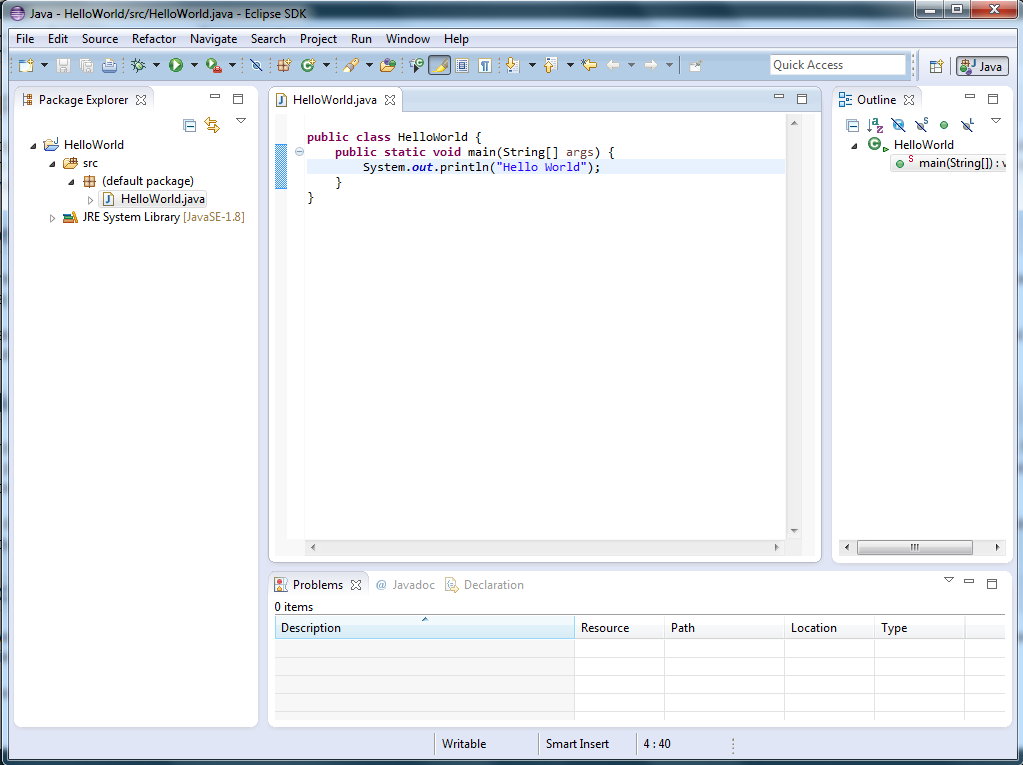
\includegraphics{eclipse.png}


\subsection{JavaFX Scene Builder}
\label{config:javafx-scene-builder}
Rekomendowaną przez firmę Oracle technologią do tworzenia graficznego interfejsu użytkownika (GUI) aplikacji pisanych w Javie jest obecnie JavaFX. Powstało w tym celu narzędzie, które znacznie ułatwia cały proces i pozwala stworzyć interfejs za pomocą przyjaznego mechanizmu drag\&drop.

Narzędzie JavaFX Scene Builder w wersji 2.0 można pobrać \href{http://www.oracle.com/technetwork/java/javase/downloads/sb2download-2177776.html}{ze strony Oracle}.

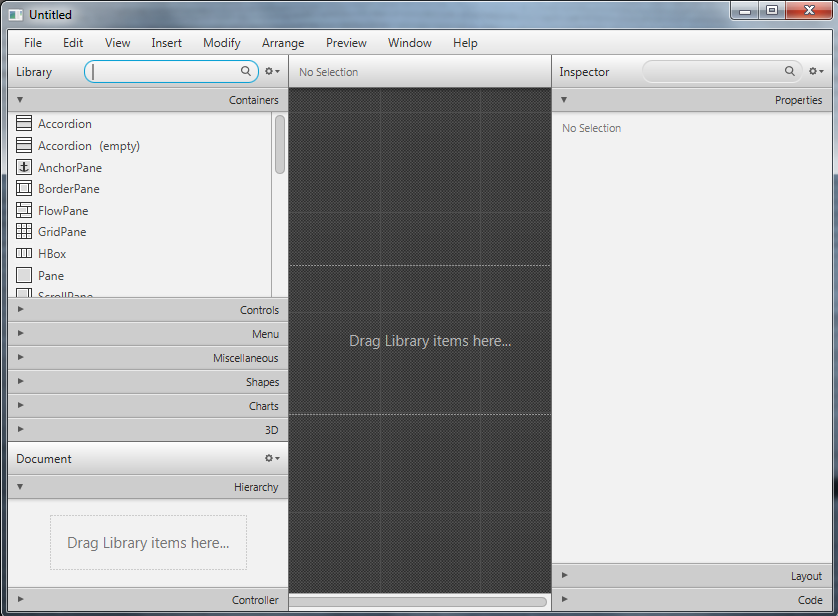
\includegraphics{scenebuilder.png}


\subsection{Rozwiązywanie problemów}
\label{config:rozwiazywanie-problemow}\begin{enumerate}
\item {} 
Sprawdzenie wersji systemu operacyjnego

\end{enumerate}

W celu sprawdzenia wersji systemu operacyjnego kliknij prawym przyciskiem myszy na opcji ``Komputer'' i wybierz właściwości. Wśród informacji znajdziesz także wersję systemu operacyjnego (32 lub 64 bit)

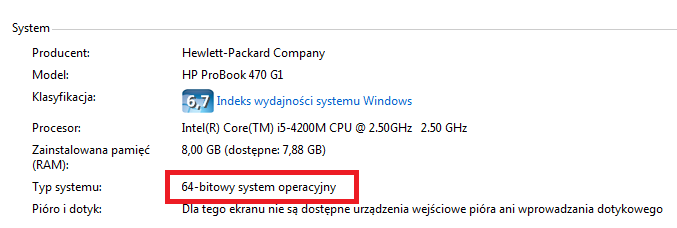
\includegraphics{bit.png}

Wszystkie wcześniej wspomniane narzędzia należy zainstalować zgodnie z wersją swojego systemu operacyjnego.
\begin{enumerate}
\setcounter{enumi}{1}
\item {} 
Konfiguracja Javy 8 w przypadku kilku jej wersji na komputerze.

\end{enumerate}

W przypadku, gdy na komputerze było wcześniej zainstalowanych kilka wersji Javy, eclipse może domyślnie korzystać z jej starszej wersji (np. 7), co na późniejszym etapie uniemożliwi nam tworzenie aplikacji z graficznym interfejsem użytkownika w Javie FX. W celu sprawdzenia i skonfigurowania odpowiedniej wersji Javy w eclipse należy przejść do opcji Window -\textgreater{} Preferences -\textgreater{} Installed JREs.

Jako domyślne środowisko uruchomieniowe powinno być to oznaczone jako 1.8.0 (z ewentualnym dopiskiem o wersji aktualizacji). Jeżeli tak nie jest należy wybrać opcję Add -\textgreater{} Standard VM a następnie wskazać główny folder zainstalowanego pakietu JDK w sekcji JRE home.

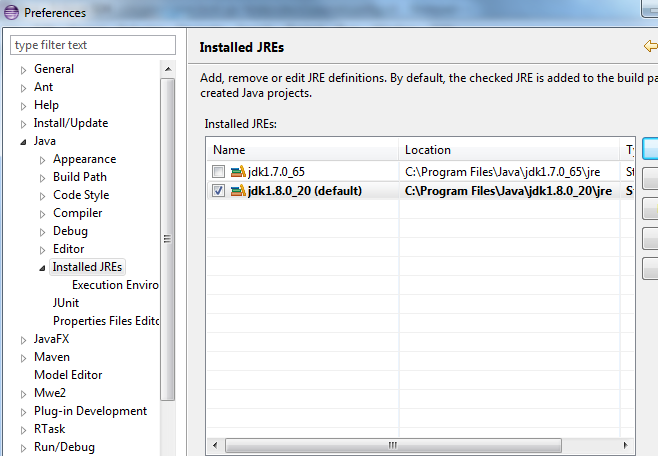
\includegraphics{eclipsejdk.png}

Powyżej widać, że skonfigurowana jest zarówno Java 7 jak i 8, ale wersja 8 ustawiona jest jako domyślna
\begin{enumerate}
\setcounter{enumi}{2}
\item {} 
Eclipse po uruchomieniu pokazuje błąd związany z wtyczką Mercurial (system kontroli wersji).

\end{enumerate}

Błąd należy zignorować, nie powinien pojawiać się przy kolejnych uruchomieniach środowiska.


\chapter{Kurs}
\label{index:ze-strony-oracle}\label{index:kurs}
Cały kurs podzielony jest na 8 lekcji.


\section{Wprowadzenie do języka Java}
\label{wprowadzenie:wprowadzenie-do-jezyka-java}\label{wprowadzenie::doc}
W lekcji tej dowiesz się:
\begin{itemize}
\item {} 
jak używać środowiska eclipse

\item {} 
co powstaje w wyniku kompilacji kodu źródłowego napisanego w języku Java

\item {} 
jak uruchamiać swoje programy

\item {} 
czym są zmienne

\item {} 
jakie są podstawowe typy danych w Javie

\item {} 
jak wykonywać podstawowe operacje arytmetyczne

\end{itemize}

Podczas lekcji nauczyciel powinien krótko omawiać daną sekcję pod względem teoretycznym, a następnie omawiać prezentowane przykłady, prosząc z wyprzedzeniem uczniów o sugestie tego jak zapisać dalszy fragment kodu źródłowego. Uczniowie powinni pisać kod jednocześnie na swoich komputerach, aby móc obserwować wynik działania aplikacji. Lekcja kończy się zadaniem do samodzielnego wykonania, które należy wykonać na zajęciach lub dokończyć samodzielnie w domu.


\subsection{Eclipse IDE}
\label{wprowadzenie:eclipse-ide}
Eclipse to najpopularniejsze środowisko programistyczne wśród programistów Java. Jego głównymi zaletami z punktu widzenia osoby początkującej jest wykrywanie błędów w trakcie pisania kodu a także podpowiadanie składni wraz z możliwością generowania i prostej modyfikacji (refaktoryzacji) kodu źródłowego. Wszystko to składa się przede wszystkim na znaczną oszczędność czasu.

Przy pierwszym uruchomieniu środowiska zostaniemy zapytani o wskazanie folderu ``workspace'' - jest to folder, w którym przechowywane będą tworzone przez nas projekty. Zalecamy zostawić tę lokalizację domyślną.

{\hfill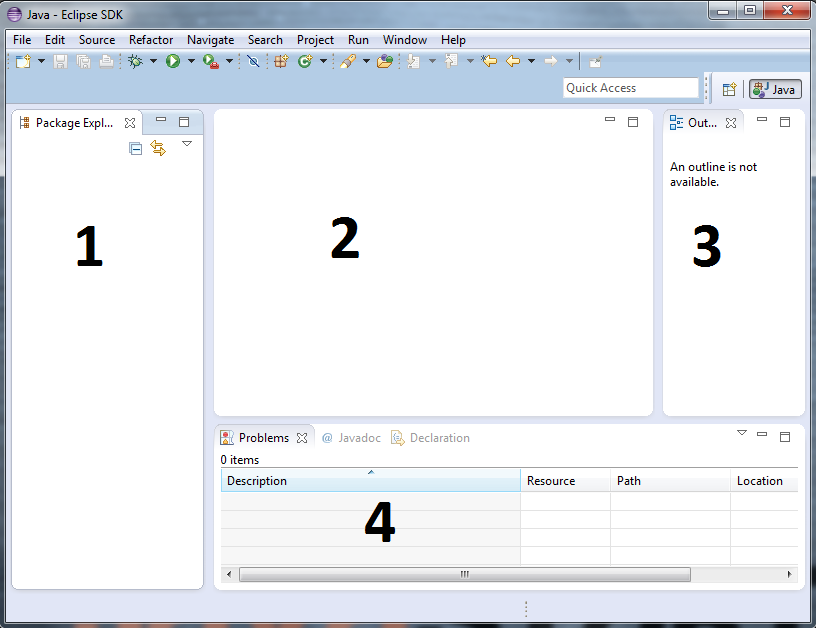
\includegraphics{eclipse_overview.png}\hfill}

Na powyższym zrzucie ekranu widać domyślny widok, który zastaniemy po uruchomieniu środowiska eclipse. Można w nim wyróżnić 4 główne obszary:
\begin{enumerate}
\item {} 
Package Explorer - w tym miejscu będziemy widzieli wszystkie projekty, które zapisane są w folderze \textbf{workspace} oraz ich strukturę w postaci rozwijanego drzewa

\item {} 
Obszar oznaczony numerem 2 to główna część robocza - w tym miejscu będziemy edytowali kod źródłowy aplikacji

\item {} 
Outline - to skrótowy podgląd danego pliku i elementów w nim zawartych (zmienne, metody/funkcje)

\item {} 
W dolnej części ekranu znajduje się kilka zakładek. Najważniejsza z nich to \textbf{Problems}, która pokazuje wszelkie błędy i ostrzeżenia występujące w kodzie źródłowym. W tym miejscu zobaczymy także dodatkową zakładkę \textbf{Console} z wydrukami generowanymi przez nasze aplikacje.

\end{enumerate}


\subsection{Pierwszy Projekt}
\label{wprowadzenie:pierwszy-projekt}
W celu utworzenia nowego projektu wybieramy opcję \textbf{File -\textgreater{} New -\textgreater{} Java Project}

{\hfill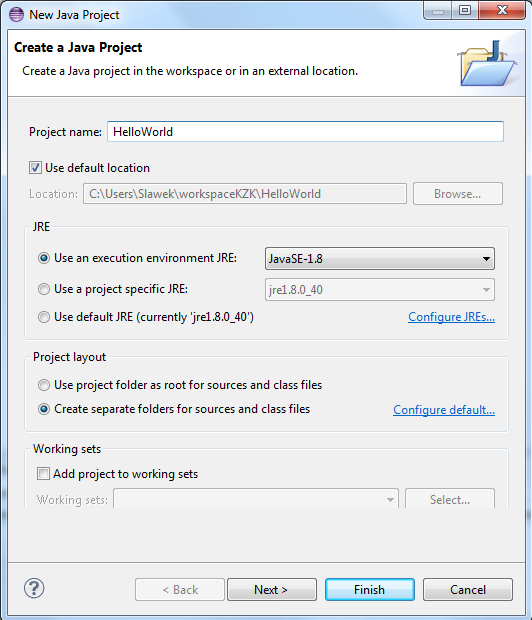
\includegraphics{eclipse_first_project.png}\hfill}

Wpisujemy dowolną nazwę projektu w polu \textbf{Project name} a także wybieramy wersję maszyny wirtualnej (JRE), na jakiej ma być uruchomiony nasz program (domyślnie JavaSE-1.8). Klikamy Finish.

W obszarze Project Explorer pojawi się nowo utworzony projekt:

{\hfill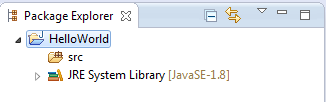
\includegraphics{hello_world.png}\hfill}

Widzimy tu folder \textbf{src}, w którym umieszczane będą pliki z kodem źródłowym, a także dołączoną wirtualną maszynę, na której nasz projekt będzie uruchamiany.

Teraz należy utworzyć plik, w którym będziemy edytowali kod źródłowy. W dalszej częściu kursu będziemy mówili krótko o tworzeniu nowej \textbf{klasy}. Klasa jest pojęciem związanym z programowaniem obiektowym, które będzie głównym zagadnieniem kolejnej lekcji.

Kliknij prawym przyciskiem na folderze src i wybierz opcję \textbf{New -\textgreater{} Class}. Można także posłużyć się wygodnym skrótem i skorzystać z przycisku z symbolem C, który znajdziemy na górnym pasku nawigacyjnym.

{\hfill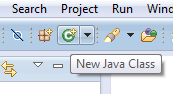
\includegraphics{new_class.png}\hfill}

W kreatorze klasy wymagane jest podanie jedynie nazwy klasy. My jednak zaznaczymy także opcję przy \textbf{public static void main(String{[}{]} args)}.

{\hfill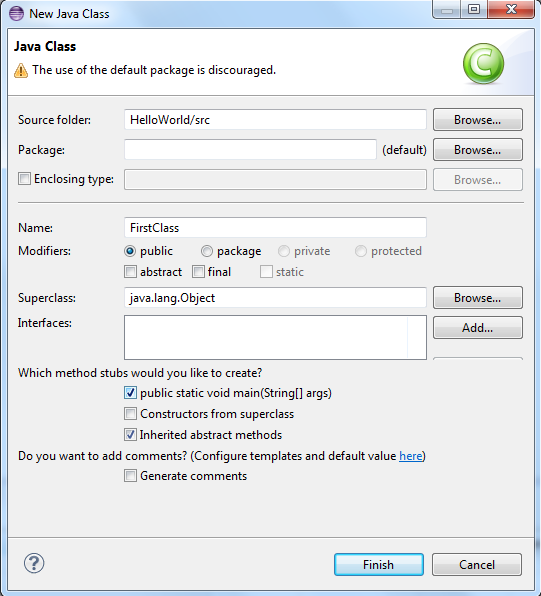
\includegraphics{class.png}\hfill}

\begin{notice}{note}{Note:}
Nazwy klas rozpoczynaj zawsze wielką literą a jeżeli nazwa składa się z kilku wyrazów to je także rozpoczynaj wielką literą, np. NazwaTwojejKlasy albo ThisIsMyClass. Pamiętaj także, że nazwa klasy musi być identyczna z nazwą pliku, w którym ta klasa się znajduje (eclipse zadba o to automatycznie).
\end{notice}

W naszym przypadku nazwą klasy jest \textbf{FirstClass}.

\begin{notice}{attention}{Attention:}
Zapamiętaj, że w Javie nazwy klas i wielkość używanych liter, mają znaczenie. ``NazwaKlasy'' i ``nazwaKlasy'' będą potraktowane jako dwa zupełnie różne elementy.
\end{notice}

W utworzonej przez nas klasie został wygenerowany następujący kod źródłowy:

\begin{Verbatim}[commandchars=\\\{\},numbers=left,firstnumber=1,stepnumber=1]
\PYG{k+kd}{public} \PYG{k+kd}{class} \PYG{n+nc}{FirstClass} \PYG{o}{\PYGZob{}}

  \PYG{k+kd}{public} \PYG{k+kd}{static} \PYG{k+kt}{void} \PYG{n+nf}{main}\PYG{o}{(}\PYG{n}{String}\PYG{o}{[}\PYG{o}{]} \PYG{n}{args}\PYG{o}{)} \PYG{o}{\PYGZob{}}
    \PYG{c+c1}{// TODO Auto\PYGZhy{}generated method stub}
    \PYG{n}{System}\PYG{o}{.}\PYG{n+na}{out}\PYG{o}{.}\PYG{n+na}{print}\PYG{o}{(}\PYG{l+s}{\PYGZdq{}Witaj Świecie!\PYGZdq{}}\PYG{o}{)}\PYG{o}{;}
  \PYG{o}{\PYGZcb{}}

\PYG{o}{\PYGZcb{}}
\end{Verbatim}

W linii 1 widzimy definicję klasy. Klasę definiujemy za pomocą słowa kluczowego \textbf{class}, po którym następuje jej nazwa. Eclipse automatycznie oznacza ją jako publiczną za pomocą słowa kluczowego \textbf{public}, co najprościej można wytłumaczyć jako możliwość jej wykorzystania z dowolnego miejsca w naszym projekcie.

W wierszu 3 widzimy zapis \emph{public static void main(String{[}{]} args)}, czyli publiczną, statyczną metodę o nazwie \textbf{main}, która nie zwraca żadnego wyniku (void). Element umieszczony w nawiasie, czyli \emph{String{[}{]} args} to argument metody main w postaci tablicy - więcej na ten temat powiemy w dalszej części lekcji.

\begin{notice}{note}{Note:}
Zapamiętaj, że od metody main rozpoczyna się działanie każdej aplikacji napisanej w języku Java. Jeżeli nie zdefiniujesz takiej metody w swojej klasie, to nie będziesz w stanie uruchomić programu.
\end{notice}

Zauważ, że zarówno definicja klasy jak i metody rozpoczyna się i końcy nawiasami klamrowymi. Nawiasy klamrowe znacznie podnoszą czytelność kodu, szczególnie, gdy klasa składa się z kilkuset, czy nawet kilku tysięcy wierszy.

W metodzie main znajduje się jeden wiersz komentarza poprzedzony znakiem podwójnego ukośnika.

\begin{notice}{note}{Note:}
Komentarze w języku Java można zapisywać na dwa sposoby. Jeżeli komentarz ma zajmować jedynie jeden wiersz poprzedź go znakiem podwójnego ukośnika. Jeżeli będzie dłuższy umieść komentarz w bloku /* komentarz {\color{red}\bfseries{}*}/ Komentarze są pomijane w trakcie kompilacji programu i nie mają wpływu na działanie aplikacji.
\end{notice}

Po komentarzu dopisaliśmy także linijkę o treści \textbf{System.out.print(``Witaj Świecie'');}, która wydrukuje na ekranie tekst podany w nawiasie, czyli Witaj Świecie.

\begin{notice}{note}{Note:}
Zapamiętaj, że każda linijka z wyrażeniem (np. drukowaniem tekstu) w języku Java musi kończyć się średnikiem.
\end{notice}

W celu uruchomienia programu wybierz z górnego paska nawigacyjnego charakterystyczny przycisk z symbolem strzałki (Run) lub po prostu użyj skrótu klawiaturowego \textbf{Ctrl+F11}.

W tym momencie w dolnej części eclipse powinno się pojawić okno konsoli (Console) z wydrukiem naszego tekstu.

{\hfill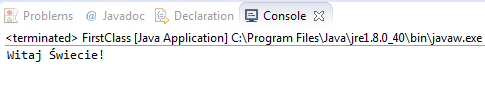
\includegraphics{run.png}\hfill}


\subsection{Typy danych}
\label{wprowadzenie:typy-danych}
W Javie tak jak w praktycznie każdym języku programowania istnieją różne typy danych. \textbf{Typ danych} to opis tego co reprezentuje dana wartość. Z powodu budowy komputera rozróżnia się liczby całkowite, liczby zmiennoprzecinkowe, znaki, ciągi znaków.
\begin{itemize}
\item {} 
boolean - typ logiczny. Może przyjmować jedynie dwie wartości - true (prawda) lub false (fałsz).

\item {} 
byte, short, int, long - typy całkowitoliczbowe. Różnią się zakresem wielkości liczby jakie mogą przechowywać (od najmniejszego do największego) - np. 1, 5, 10, 3456.

\item {} 
float, double - typy zmiennoprzecinkowe o różnym zakresie (double może przechowywać większe liczby). Separatorem dziesiętnym jest kropka, np. 3.14, 276.24563.

\item {} 
char - typ znakowy, reprezentuje pojedyncze litery lub znaki. Wartości tego typu umieszczamy pomiędzy znakami pojedynczego cudzysłowu, np. `a', `\&'.

\item {} 
String - (pisany z wielkie litery) - specjalny typ, który służy do przechowywania ciągów znaków. Ciągi znaków zapisujemy pomiędzy podwójnymi cudzysłowami, np. ``Ania'', ``Jakiś dowolny tekst''.

\end{itemize}

\textbf{Ćwiczenie (5 min)}

Napisz program, który wydrukuje na ekranie następujące wartości (wykorzystaj różne typy danych):

\begin{Verbatim}[commandchars=\\\{\}]
245
123.456
a
Java jest cool
\end{Verbatim}

\emph{plik DataTypes.java}

\begin{Verbatim}[commandchars=\\\{\},numbers=left,firstnumber=1,stepnumber=1]
\PYG{k+kd}{public} \PYG{k+kd}{class} \PYG{n+nc}{FirstClass} \PYG{o}{\PYGZob{}}
  \PYG{k+kd}{public} \PYG{k+kd}{static} \PYG{k+kt}{void} \PYG{n+nf}{main}\PYG{o}{(}\PYG{n}{String}\PYG{o}{[}\PYG{o}{]} \PYG{n}{args}\PYG{o}{)} \PYG{o}{\PYGZob{}}
    \PYG{n}{System}\PYG{o}{.}\PYG{n+na}{out}\PYG{o}{.}\PYG{n+na}{println}\PYG{o}{(}\PYG{l+m+mi}{245}\PYG{o}{)}\PYG{o}{;}
    \PYG{n}{System}\PYG{o}{.}\PYG{n+na}{out}\PYG{o}{.}\PYG{n+na}{println}\PYG{o}{(}\PYG{l+m+mf}{123.456}\PYG{o}{)}\PYG{o}{;}
    \PYG{n}{System}\PYG{o}{.}\PYG{n+na}{out}\PYG{o}{.}\PYG{n+na}{println}\PYG{o}{(}\PYG{l+s+sc}{\PYGZsq{}a\PYGZsq{}}\PYG{o}{)}\PYG{o}{;}
    \PYG{n}{System}\PYG{o}{.}\PYG{n+na}{out}\PYG{o}{.}\PYG{n+na}{println}\PYG{o}{(}\PYG{l+s}{\PYGZdq{}Java jest cool\PYGZdq{}}\PYG{o}{)}\PYG{o}{;}
  \PYG{o}{\PYGZcb{}}
\PYG{o}{\PYGZcb{}}
\end{Verbatim}


\subsection{Zmienne}
\label{wprowadzenie:zmienne}
Drukowanie danych, na których nie możemy wykonywać żadnych działań, czy po prostu zapamiętać w pamięci komputera nie byłoby zbyt użyteczne. Na szczęście w Javie możemy tworzyć tzw. \textbf{zmienne}, czyli takie elementy, które pozwalają na przechowywanie wartości różnych typów danych. Java w odróżnieniu od np. PHP jest językiem statycznie typowanym co oznacza, że zmienna musi mieć określony typ. Jeżeli chcesz przechowywać w niej wartość zmiennoprzecinkową, to nie możesz jej zadeklarować jako int, ponieważ spowoduje to błąd kompilacji.

Tworzenie zmiennej możemy podzielić na dwa etapy:
\begin{itemize}
\item {} 
deklarację - w tym momencie następuje zaalokowanie pamięci w komputerze

\item {} 
inicjalizację (inicjację) - w tym momencie następuje przypisanie konkretnej wartości do zmiennej

\end{itemize}

Dwa wyżej wspomniane etapy mogą być od siebie oddzielone lub też można je połączyć ze sobą.

\emph{plik Variables.java}

\begin{Verbatim}[commandchars=\\\{\},numbers=left,firstnumber=1,stepnumber=1]
\PYG{k+kd}{public} \PYG{k+kd}{class} \PYG{n+nc}{Variables} \PYG{o}{\PYGZob{}}
  \PYG{k+kd}{public} \PYG{k+kd}{static} \PYG{k+kt}{void} \PYG{n+nf}{main}\PYG{o}{(}\PYG{n}{String}\PYG{o}{[}\PYG{o}{]} \PYG{n}{args}\PYG{o}{)} \PYG{o}{\PYGZob{}}
    \PYG{c+c1}{// deklaracja zmiennych różnego typu}
    \PYG{k+kt}{int} \PYG{n}{x}\PYG{o}{;}
    \PYG{k+kt}{double} \PYG{n}{num}\PYG{o}{;}
    \PYG{k+kt}{char} \PYG{n}{letter}\PYG{o}{;}
    \PYG{n}{String} \PYG{n}{napis}\PYG{o}{;}

    \PYG{c+c1}{// inicjalizacja zmiennych}
    \PYG{n}{x} \PYG{o}{=} \PYG{l+m+mi}{5}\PYG{o}{;}
    \PYG{n}{num} \PYG{o}{=} \PYG{l+m+mf}{12.67}\PYG{o}{;}
    \PYG{n}{letter} \PYG{o}{=} \PYG{l+s+sc}{\PYGZsq{}b\PYGZsq{}}\PYG{o}{;}
    \PYG{n}{napis} \PYG{o}{=} \PYG{l+s}{\PYGZdq{}To może być bardzo długie zdanie\PYGZdq{}}\PYG{o}{;}

    \PYG{c+c1}{// deklaracja połączona z inicjalizacją}
    \PYG{k+kt}{int} \PYG{n}{y} \PYG{o}{=} \PYG{l+m+mi}{15}\PYG{o}{;}
    \PYG{n}{String} \PYG{n}{zdanie} \PYG{o}{=} \PYG{l+s}{\PYGZdq{}To jest przykładowe zdanie\PYGZdq{}}\PYG{o}{;}
  \PYG{o}{\PYGZcb{}}
\PYG{o}{\PYGZcb{}}
\end{Verbatim}

\textbf{Ćwiczenie (5 min)}

Napisz program podobny do tego z poprzedniego zadania - wydrukuj na ekranie kilka wartości różnego typu, ale tym razem skorzystaj także ze zmiennych.

\emph{plik DataTypesVars.java}

\begin{Verbatim}[commandchars=\\\{\},numbers=left,firstnumber=1,stepnumber=1]
\PYG{k+kd}{public} \PYG{k+kd}{class} \PYG{n+nc}{DataTypesVars} \PYG{o}{\PYGZob{}}
  \PYG{k+kd}{public} \PYG{k+kd}{static} \PYG{k+kt}{void} \PYG{n+nf}{main}\PYG{o}{(}\PYG{n}{String}\PYG{o}{[}\PYG{o}{]} \PYG{n}{args}\PYG{o}{)} \PYG{o}{\PYGZob{}}
    \PYG{k+kt}{int} \PYG{n}{num1} \PYG{o}{=} \PYG{l+m+mi}{123}\PYG{o}{;}
    \PYG{k+kt}{double} \PYG{n}{num2} \PYG{o}{=} \PYG{l+m+mf}{567.123}\PYG{o}{;}
    \PYG{k+kt}{char} \PYG{n}{b} \PYG{o}{=} \PYG{l+s+sc}{\PYGZsq{}b\PYGZsq{}}\PYG{o}{;}
    \PYG{n}{String} \PYG{n}{name} \PYG{o}{=} \PYG{l+s}{\PYGZdq{}Jan Kowalski\PYGZdq{}}\PYG{o}{;}

    \PYG{n}{System}\PYG{o}{.}\PYG{n+na}{out}\PYG{o}{.}\PYG{n+na}{println}\PYG{o}{(}\PYG{n}{num1}\PYG{o}{)}\PYG{o}{;}
    \PYG{n}{System}\PYG{o}{.}\PYG{n+na}{out}\PYG{o}{.}\PYG{n+na}{println}\PYG{o}{(}\PYG{n}{num2}\PYG{o}{)}\PYG{o}{;}
    \PYG{n}{System}\PYG{o}{.}\PYG{n+na}{out}\PYG{o}{.}\PYG{n+na}{println}\PYG{o}{(}\PYG{n}{b}\PYG{o}{)}\PYG{o}{;}
    \PYG{n}{System}\PYG{o}{.}\PYG{n+na}{out}\PYG{o}{.}\PYG{n+na}{println}\PYG{o}{(}\PYG{n}{name}\PYG{o}{)}\PYG{o}{;}
  \PYG{o}{\PYGZcb{}}
\PYG{o}{\PYGZcb{}}
\end{Verbatim}


\subsection{Operacje arytmetyczne i logiczne}
\label{wprowadzenie:operacje-arytmetyczne-i-logiczne}
Jednymi z najważniejszych elementów w jakich wykorzystujemy komputery są obliczenia. Nie zawsze muszą to być skomplikowane rachunki matematyczne - czasami chcemy coś po prostu przesunąć o 1 piksel w prawo na ekranie (np. w grach), a innym razem zwiększyć wiek użytkownika o 1, gdy ma urodziny.

W języku Java znajdziemy wszystkie najpopularniejsze operatory arytmetyczno logiczne:
\begin{itemize}
\item {} 
\textbf{+, -} - dodawanie i odejmowanie liczb

\item {} 
\textbf{*, /} - mnożenie i dzielenie całkowite liczb

\item {} 
\textbf{\%} - dzielenie modulo (reszta z dzielenia)

\item {} 
\textbf{\&\&} - koniunkcja logiczna. Tylko PRAWDA \&\& PRAWDA da w wyniku PRAWDA

\item {} 
\textbf{\textbar{}\textbar{}} - alternatywa logiczna. Co najmniej jedna składowa musi być PRAWDĄ, aby wynik całego wyrażenia był prawdą. PRAWDA\textbar{}\textbar{}PRAWDA lub PRAWDA\textbar{}\textbar{}FAŁSZ lub FAŁSZ\textbar{}\textbar{}PRAWDA ale nie FAŁSZ\textbar{}\textbar{}FAŁSZ

\item {} 
\textbf{\textgreater{}, \textgreater{}=, \textless{}, \textless{}=} - porównania. Większe, większe lub równe, mniejsze, mniejsze lub równe.

\item {} 
\textbf{==} - porównanie równości

\end{itemize}

Wyniki wyrażeń arytmetyczno logicznych mogą być obliczane na podstawie zmiennych lub wartości, a także przypisywane do innych zmiennych.

\emph{plik Arithmetic.java}

\begin{Verbatim}[commandchars=\\\{\},numbers=left,firstnumber=1,stepnumber=1]
\PYG{k+kd}{public} \PYG{k+kd}{class} \PYG{n+nc}{Arithmetic} \PYG{o}{\PYGZob{}}
  \PYG{k+kd}{public} \PYG{k+kd}{static} \PYG{k+kt}{void} \PYG{n+nf}{main}\PYG{o}{(}\PYG{n}{String}\PYG{o}{[}\PYG{o}{]} \PYG{n}{args}\PYG{o}{)} \PYG{o}{\PYGZob{}}
    \PYG{k+kt}{int} \PYG{n}{num1} \PYG{o}{=} \PYG{l+m+mi}{5}\PYG{o}{;}
    \PYG{k+kt}{int} \PYG{n}{num2} \PYG{o}{=} \PYG{l+m+mi}{3}\PYG{o}{;}
    \PYG{c+c1}{//jaki jest wynik działania num1*num2 ?}
    \PYG{k+kt}{int} \PYG{n}{num3} \PYG{o}{=} \PYG{n}{num1} \PYG{o}{*} \PYG{n}{num2}\PYG{o}{;}
    \PYG{n}{System}\PYG{o}{.}\PYG{n+na}{out}\PYG{o}{.}\PYG{n+na}{println}\PYG{o}{(}\PYG{n}{num3}\PYG{o}{)}\PYG{o}{;}

    \PYG{c+c1}{//czy zmienna num1 jest większa od 3 ?}
    \PYG{k+kt}{boolean} \PYG{n}{validate} \PYG{o}{=} \PYG{n}{num1} \PYG{o}{\PYGZgt{}} \PYG{l+m+mi}{3}\PYG{o}{;}
    \PYG{n}{System}\PYG{o}{.}\PYG{n+na}{out}\PYG{o}{.}\PYG{n+na}{println}\PYG{o}{(}\PYG{n}{validate}\PYG{o}{)}\PYG{o}{;}
  \PYG{o}{\PYGZcb{}}
\PYG{o}{\PYGZcb{}}
\end{Verbatim}

Znak dodawania (+) ma również specjalne zastosowanie w przypadku ciągów znaków (typ String). Powoduje on złączenie (konkatenację) dwóch ciągów znaków i utworzenie na ich podstawie nowego napisu.

\begin{Verbatim}[commandchars=\\\{\}]
\PYG{n}{String} \PYG{n}{napis} \PYG{o}{=} \PYG{l+s}{\PYGZdq{}Jan\PYGZdq{}} \PYG{o}{+} \PYG{l+s}{\PYGZdq{}Kowalski\PYGZdq{}}\PYG{o}{;}
\end{Verbatim}

\textbf{Ćwiczenie (10 min)}
Napisz prosty kalkulator. Zadeklaruj i zainicjuj dwie liczby typu zmiennoprzecinkowego a następnie wyświetl na ekranie wynik ich dodawania, odejmowania, mnożenia i dzielenia. Dodatkowo wyświetl na ekranie, czy pierwsza z liczb jest większa od drugiej, a także, czy ich iloczyn jest większy od 100.
Przykładowy wydruk programu:

\begin{Verbatim}[commandchars=\\\{\}]
a + b = 28.3
a \PYGZhy{} b = 18.7
a * b = 112.8
a / b = 4.895833333333334
A \PYGZgt{} B ?true
A * B \PYGZgt{} 100 ? true
\end{Verbatim}

\emph{plik SimpleCalculator.java}

\begin{Verbatim}[commandchars=\\\{\},numbers=left,firstnumber=1,stepnumber=1]
\PYG{k+kd}{public} \PYG{k+kd}{class} \PYG{n+nc}{SimpleCalculator} \PYG{o}{\PYGZob{}}
  \PYG{k+kd}{public} \PYG{k+kd}{static} \PYG{k+kt}{void} \PYG{n+nf}{main}\PYG{o}{(}\PYG{n}{String}\PYG{o}{[}\PYG{o}{]} \PYG{n}{args}\PYG{o}{)} \PYG{o}{\PYGZob{}}
    \PYG{k+kt}{double} \PYG{n}{a} \PYG{o}{=} \PYG{l+m+mf}{23.5}\PYG{o}{;}
    \PYG{k+kt}{double} \PYG{n}{b} \PYG{o}{=} \PYG{l+m+mf}{4.8}\PYG{o}{;}

    \PYG{n}{System}\PYG{o}{.}\PYG{n+na}{out}\PYG{o}{.}\PYG{n+na}{println}\PYG{o}{(}\PYG{l+s}{\PYGZdq{}a + b = \PYGZdq{}} \PYG{o}{+} \PYG{o}{(}\PYG{n}{a} \PYG{o}{+} \PYG{n}{b}\PYG{o}{)}\PYG{o}{)}\PYG{o}{;}
    \PYG{n}{System}\PYG{o}{.}\PYG{n+na}{out}\PYG{o}{.}\PYG{n+na}{println}\PYG{o}{(}\PYG{l+s}{\PYGZdq{}a \PYGZhy{} b = \PYGZdq{}} \PYG{o}{+} \PYG{o}{(}\PYG{n}{a} \PYG{o}{\PYGZhy{}} \PYG{n}{b}\PYG{o}{)}\PYG{o}{)}\PYG{o}{;}
    \PYG{n}{System}\PYG{o}{.}\PYG{n+na}{out}\PYG{o}{.}\PYG{n+na}{println}\PYG{o}{(}\PYG{l+s}{\PYGZdq{}a * b = \PYGZdq{}} \PYG{o}{+} \PYG{o}{(}\PYG{n}{a} \PYG{o}{*} \PYG{n}{b}\PYG{o}{)}\PYG{o}{)}\PYG{o}{;}
    \PYG{n}{System}\PYG{o}{.}\PYG{n+na}{out}\PYG{o}{.}\PYG{n+na}{println}\PYG{o}{(}\PYG{l+s}{\PYGZdq{}a / b = \PYGZdq{}} \PYG{o}{+} \PYG{o}{(}\PYG{n}{a} \PYG{o}{/} \PYG{n}{b}\PYG{o}{)}\PYG{o}{)}\PYG{o}{;}
    \PYG{n}{System}\PYG{o}{.}\PYG{n+na}{out}\PYG{o}{.}\PYG{n+na}{println}\PYG{o}{(}\PYG{l+s}{\PYGZdq{}A \PYGZgt{} B ?\PYGZdq{}} \PYG{o}{+} \PYG{o}{(}\PYG{n}{a} \PYG{o}{\PYGZgt{}} \PYG{n}{b}\PYG{o}{)}\PYG{o}{)}\PYG{o}{;}
    \PYG{n}{System}\PYG{o}{.}\PYG{n+na}{out}\PYG{o}{.}\PYG{n+na}{println}\PYG{o}{(}\PYG{l+s}{\PYGZdq{}A * B \PYGZgt{} 100 ? \PYGZdq{}} \PYG{o}{+} \PYG{o}{(}\PYG{n}{a}\PYG{o}{*}\PYG{n}{b} \PYG{o}{\PYGZgt{}} \PYG{l+m+mi}{100}\PYG{o}{)}\PYG{o}{)}\PYG{o}{;}
  \PYG{o}{\PYGZcb{}}
\PYG{o}{\PYGZcb{}}
\end{Verbatim}

Zauważ, że w powyższym przykładzie konkatenacji a nawet obliczeń dokonujemy bezpośrednio w metodzie drukującej wynik na ekranie. Warto zwrócić także uwagę na to, że wartość typu String możemy łączyć z wartościami innego typu i zostaną one automatycznie dołączone do naszego napisu. Jeżeli wykorzystałeś dodatkowe zmienne do przechowywania wyników poszczególnych działań - nie jest to błędem.


\subsection{Tablice jednowymiarowe}
\label{wprowadzenie:tablice-jednowymiarowe}
Zmienne nadają się świetnie do przechowywania pojedynczych wartości, jednak jeżeli w swoim programie posiadasz pewien zbiór danych, niezbędne będzie zastosowanie czegoś bardziej wygodnego. W końcu zapisywanie 100 liczb w postaci:

\begin{Verbatim}[commandchars=\\\{\}]
int x1 = 1;
int x2 = 2;
int x3 = 3;
//itd.
\end{Verbatim}

nie byłoby zbyt wygodne, prawda?
Podstawowym elementem, który pozwala rozwiązać ten problem w programowaniu są tablice.

\begin{notice}{note}{Note:}
Tablica to specjalny typ danych, który pozwala przechowywać duże ilości wartości tego samego typu.
\end{notice}

Deklaracja i inicjalizacja tablic jest bardzo podobna do zwykłych zmiennych:

Powyżej zadeklarowano i utworzono tablicę 5 liczb całkowitych typu int, która może przechowywać 5 wartości oraz tablicę typu String, która może przechowywać 10 napisów.

W przypadku, gdy z góry znasz wartości, którymi chcesz uzupełnić tablicę, istnieje szybki sposób na jej inicjalizację poprzez wymienienie wszystkich wartości w trakcie tworzenia tablicy:

\begin{Verbatim}[commandchars=\\\{\}]
int[] numbers = new int[]\PYGZob{}1, 2, 3, 4, 5\PYGZcb{};
\end{Verbatim}

Zauważ, że w takim przypadku nie jest konieczne określanie rozmiaru tablicy w nawiasach kwadratowych, ponieważ maszyna wirtualna wywnioskuje to sama na podstawie ilości podanych elementów.

W wielu przypadkach tablica będzie tworzona na podstawie rozmiaru, który użytkownik wprowadzi np. z klawiatury i nie będziemy go znali w dalszej części kodu. W takiej sytuacji możemy jednak skorzystać z wartości \textbf{length}, którą posiada każda tablica niezależnie od tego jakiego jest typu.

\begin{Verbatim}[commandchars=\\\{\}]
int[] tab = new int[5];
int size = tab.length;
System.out.print(size);
\end{Verbatim}

\begin{notice}{note}{Note:}
Zapamiętaj jednak, że właściwość length zwraca całkowity rozmiar tablicy, a nie to ile rzeczywiście elementów jest do niej wpisanych.
\end{notice}

W celu przypisania lub odwołania się do poszczególnych komórek takich tablic należy odwołać się do nich poprzez indeksy:

\emph{plik Tabs.java}

\begin{Verbatim}[commandchars=\\\{\},numbers=left,firstnumber=1,stepnumber=1]
\PYG{k+kd}{public} \PYG{k+kd}{class} \PYG{n+nc}{Tabs} \PYG{o}{\PYGZob{}}
    \PYG{k+kd}{public} \PYG{k+kd}{static} \PYG{k+kt}{void} \PYG{n+nf}{main}\PYG{o}{(}\PYG{n}{String}\PYG{o}{[}\PYG{o}{]} \PYG{n}{args}\PYG{o}{)} \PYG{o}{\PYGZob{}}
        \PYG{k+kt}{int}\PYG{o}{[}\PYG{o}{]} \PYG{n}{tab} \PYG{o}{=} \PYG{k}{new} \PYG{k+kt}{int}\PYG{o}{[}\PYG{l+m+mi}{5}\PYG{o}{]}\PYG{o}{;}
        \PYG{n}{String}\PYG{o}{[}\PYG{o}{]} \PYG{n}{words} \PYG{o}{=} \PYG{k}{new} \PYG{n}{String}\PYG{o}{[}\PYG{l+m+mi}{10}\PYG{o}{]}\PYG{o}{;}

        \PYG{c+c1}{// tablice posiadają indeksy numerowane od 0}
        \PYG{n}{tab}\PYG{o}{[}\PYG{l+m+mi}{0}\PYG{o}{]} \PYG{o}{=} \PYG{l+m+mi}{1}\PYG{o}{;}
        \PYG{n}{tab}\PYG{o}{[}\PYG{l+m+mi}{1}\PYG{o}{]} \PYG{o}{=} \PYG{l+m+mi}{2}\PYG{o}{;}

        \PYG{c+c1}{// ale elementów nie musimy uzupełniać w określonym porządku}
        \PYG{n}{words}\PYG{o}{[}\PYG{l+m+mi}{0}\PYG{o}{]} \PYG{o}{=} \PYG{l+s}{\PYGZdq{}Ala\PYGZdq{}}\PYG{o}{;}
        \PYG{n}{words}\PYG{o}{[}\PYG{l+m+mi}{3}\PYG{o}{]} \PYG{o}{=} \PYG{l+s}{\PYGZdq{}kot\PYGZdq{}}\PYG{o}{;}

        \PYG{n}{System}\PYG{o}{.}\PYG{n+na}{out}\PYG{o}{.}\PYG{n+na}{println}\PYG{o}{(}\PYG{l+s}{\PYGZdq{}Pierwszy element tablicy tab[] = \PYGZdq{}} \PYG{o}{+} \PYG{n}{tab}\PYG{o}{[}\PYG{l+m+mi}{0}\PYG{o}{]}\PYG{o}{)}\PYG{o}{;}
        \PYG{n}{System}\PYG{o}{.}\PYG{n+na}{out}\PYG{o}{.}\PYG{n+na}{println}\PYG{o}{(}\PYG{l+s}{\PYGZdq{}Czwarty element tablicy words[] = \PYGZdq{}} \PYG{o}{+} \PYG{n}{words}\PYG{o}{[}\PYG{l+m+mi}{3}\PYG{o}{]}\PYG{o}{)}\PYG{o}{;}
    \PYG{o}{\PYGZcb{}}
\PYG{o}{\PYGZcb{}}
\end{Verbatim}

\begin{notice}{attention}{Attention:}
Zapamiętaj, że tablice tak jak i praktycznie wszystkie inne struktury danych w Javie są indeksowane zaczynając od 0, a nie od 1.
\end{notice}

Rozmiaru tablic niestety nie da się zmienić, więc jeżeli uznasz, że zabrakło Ci w niej miejsca, będziesz musiał utworzyć nową, większą tablicę.

\textbf{Ćwiczenie (10 min)}

Napisz program, w którym utworzysz tablicę 10 losowo wybranych przez siebie liczb zmiennoprzecinkowych. Wydrukuj na ekranie:
\begin{itemize}
\item {} 
wszystkie wartości,

\item {} 
sumę wartości zapisanych na pozycjach nieparzystych tablicy(pierwszy, trzeci, piąty ... element tablicy)

\item {} 
ostatni element tablicy (wykorzystaj właściwość length)

\end{itemize}

\begin{Verbatim}[commandchars=\\\{\},numbers=left,firstnumber=1,stepnumber=1]
\PYG{k+kd}{public} \PYG{k+kd}{class} \PYG{n+nc}{TabCalculator} \PYG{o}{\PYGZob{}}
    \PYG{k+kd}{public} \PYG{k+kd}{static} \PYG{k+kt}{void} \PYG{n+nf}{main}\PYG{o}{(}\PYG{n}{String}\PYG{o}{[}\PYG{o}{]} \PYG{n}{args}\PYG{o}{)} \PYG{o}{\PYGZob{}}
        \PYG{k+kt}{double}\PYG{o}{[}\PYG{o}{]} \PYG{n}{nums} \PYG{o}{=} \PYG{k}{new} \PYG{k+kt}{double}\PYG{o}{[}\PYG{o}{]} \PYG{o}{\PYGZob{}} \PYG{l+m+mf}{2.5}\PYG{o}{,} \PYG{l+m+mf}{15.7}\PYG{o}{,} \PYG{l+m+mf}{1024.6}\PYG{o}{,} \PYG{l+m+mi}{33}\PYG{o}{,} \PYG{l+m+mf}{56.82}\PYG{o}{,} \PYG{l+m+mf}{1.1}\PYG{o}{,}
                \PYG{l+m+mf}{23.90}\PYG{o}{,} \PYG{l+m+mf}{999.25}\PYG{o}{,} \PYG{l+m+mf}{550.6}\PYG{o}{,} \PYG{l+m+mf}{15.7} \PYG{o}{\PYGZcb{}}\PYG{o}{;}

        \PYG{n}{System}\PYG{o}{.}\PYG{n+na}{out}\PYG{o}{.}\PYG{n+na}{println}\PYG{o}{(}\PYG{l+s}{\PYGZdq{}Elementy tablicy: \PYGZdq{}}\PYG{o}{)}\PYG{o}{;}
        \PYG{n}{System}\PYG{o}{.}\PYG{n+na}{out}\PYG{o}{.}\PYG{n+na}{println}\PYG{o}{(}\PYG{n}{nums}\PYG{o}{[}\PYG{l+m+mi}{0}\PYG{o}{]} \PYG{o}{+} \PYG{l+s}{\PYGZdq{} \PYGZdq{}} \PYG{o}{+} \PYG{n}{nums}\PYG{o}{[}\PYG{l+m+mi}{1}\PYG{o}{]} \PYG{o}{+} \PYG{l+s}{\PYGZdq{} \PYGZdq{}} \PYG{o}{+} \PYG{n}{nums}\PYG{o}{[}\PYG{l+m+mi}{2}\PYG{o}{]} \PYG{o}{+} \PYG{l+s}{\PYGZdq{} \PYGZdq{}}
                \PYG{o}{+} \PYG{n}{nums}\PYG{o}{[}\PYG{l+m+mi}{3}\PYG{o}{]} \PYG{o}{+} \PYG{l+s}{\PYGZdq{} \PYGZdq{}} \PYG{o}{+} \PYG{n}{nums}\PYG{o}{[}\PYG{l+m+mi}{4}\PYG{o}{]} \PYG{o}{+} \PYG{l+s}{\PYGZdq{} \PYGZdq{}} \PYG{o}{+} \PYG{n}{nums}\PYG{o}{[}\PYG{l+m+mi}{5}\PYG{o}{]} \PYG{o}{+} \PYG{l+s}{\PYGZdq{} \PYGZdq{}} \PYG{o}{+} \PYG{n}{nums}\PYG{o}{[}\PYG{l+m+mi}{6}\PYG{o}{]} \PYG{o}{+} \PYG{l+s}{\PYGZdq{} \PYGZdq{}}
                \PYG{o}{+} \PYG{n}{nums}\PYG{o}{[}\PYG{l+m+mi}{7}\PYG{o}{]} \PYG{o}{+} \PYG{l+s}{\PYGZdq{} \PYGZdq{}} \PYG{o}{+} \PYG{n}{nums}\PYG{o}{[}\PYG{l+m+mi}{8}\PYG{o}{]} \PYG{o}{+} \PYG{l+s}{\PYGZdq{} \PYGZdq{}} \PYG{o}{+} \PYG{n}{nums}\PYG{o}{[}\PYG{l+m+mi}{9}\PYG{o}{]}\PYG{o}{)}\PYG{o}{;}

        \PYG{k+kt}{double} \PYG{n}{sum} \PYG{o}{=} \PYG{n}{nums}\PYG{o}{[}\PYG{l+m+mi}{0}\PYG{o}{]} \PYG{o}{+} \PYG{n}{nums}\PYG{o}{[}\PYG{l+m+mi}{2}\PYG{o}{]} \PYG{o}{+} \PYG{n}{nums}\PYG{o}{[}\PYG{l+m+mi}{4}\PYG{o}{]} \PYG{o}{+} \PYG{n}{nums}\PYG{o}{[}\PYG{l+m+mi}{6}\PYG{o}{]} \PYG{o}{+} \PYG{n}{nums}\PYG{o}{[}\PYG{l+m+mi}{8}\PYG{o}{]}\PYG{o}{;}
        \PYG{n}{System}\PYG{o}{.}\PYG{n+na}{out}\PYG{o}{.}\PYG{n+na}{println}\PYG{o}{(}\PYG{l+s}{\PYGZdq{}Suma elementów na indeksach nieparzystych: \PYGZdq{}} \PYG{o}{+} \PYG{n}{sum}\PYG{o}{)}\PYG{o}{;}

        \PYG{n}{System}\PYG{o}{.}\PYG{n+na}{out}\PYG{o}{.}\PYG{n+na}{println}\PYG{o}{(}\PYG{l+s}{\PYGZdq{}Ostatni element tablicy: \PYGZdq{}} \PYG{o}{+} \PYG{n}{nums}\PYG{o}{[}\PYG{n}{nums}\PYG{o}{.}\PYG{n+na}{length}\PYG{o}{\PYGZhy{}}\PYG{l+m+mi}{1}\PYG{o}{]}\PYG{o}{)}\PYG{o}{;}
    \PYG{o}{\PYGZcb{}}
\PYG{o}{\PYGZcb{}}
\end{Verbatim}

W ćwiczeniu można było napotkać na kilka problemów. Zarówno w pierwszym jak i drugim podpunkcie należy pamiętać o indeksowaniu tablic zaczynając od 0. Do nieparzystych elementów tablicy odwołujemy się poprzez parzyste indeksy (bo zaczynają się od 0). Z kolei w trzecim punkcie należy pamiętać o tym, że właściwość length zwraca rzeczywisty rozmiar tablicy, a ponieważ indeksy numerowane są od 0, to ostatnim indeksem, do którego możemy się odwołać jest \textbf{length-1}.

\begin{notice}{attention}{Attention:}
W przypadku, gdy spróbujesz odwołać się do indeksu tablicy większego od \textbf{length-1} otrzymasz wyjątek ArrayIndexOutOfBoundsException. Jest to jeden z częściej popełnianych błędów przez młodych programistów. Może on sprawiać początkowo problemy, ponieważ jest błędem fazy wykonania aplikacji, a nie kompilacji - eclipse nie powiadomi nas więc o tym problemie w trakcie pisania kodu.
\end{notice}


\subsection{Tablice wielowymiarowe}
\label{wprowadzenie:tablice-wielowymiarowe}
Tablice jednowymiarowe znacząco usprawniają przechowywanie danych w naszej aplikacji, ponieważ nie musimy już deklarować dużej ilości zmiennych. Wyobraź sobie jednak sytuację, gdy tworzysz \href{http://pl.wikipedia.org/wiki/Okr\%C4\%99ty}{grę w okręty}:

{\hfill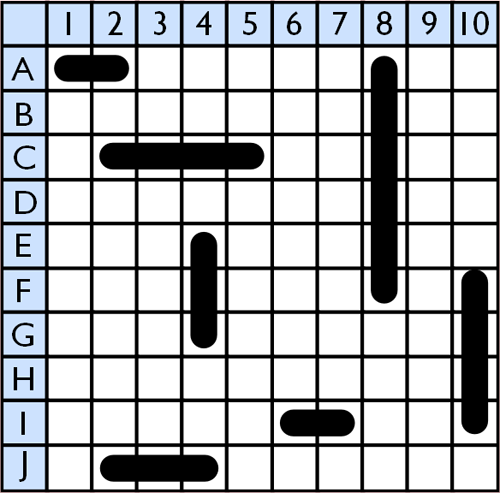
\includegraphics{ships.png}\hfill}

Możliwe, że przychodzi Ci teraz do głowy pomysł, aby wykorzystać w niej kilka tablic jednowymiarowych, które będą reprezentowały kolejne wiersze planszy. Słusznie, jednak w sytuacji, gdy będziemy chcieli utworzyć planszę o rozmiarze 20x20 komórek, niezbędne będzie zadeklarowanie 20 tablic, np.:

\begin{Verbatim}[commandchars=\\\{\}]
int[] w0 = new int[20];
int[] w1 = new int[20];
//...
int[] w19 = new int[20];
\end{Verbatim}

Przy tablicach jednowymiarowych stwierdziliśmy jednak, że tablica to taki typ danych, który pozwala przechowywać większe ilości wartości tego samego typu. Nic więc nie stoi na przeszkodzie, żeby w tablicy przechowywać inne tablice, a tym samym utworzyć \textbf{tablicę wielowymiarową}.

Tablicę taką najłatwiej wyobrazić sobie jako siatkę o rozmiarze x na y:

{\hfill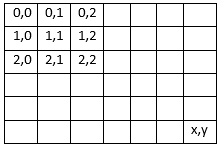
\includegraphics{multiarray.png}\hfill}

Zauważ kilka rzeczy:
\begin{itemize}
\item {} 
tablica wielowymiarowa nie musi mieć takiej samej liczby wierszy co kolumn

\item {} 
poszczególne wiersze mogą przechowywać różne ilości elementów

\end{itemize}

Przykład:

\emph{plik MultiArray.java}

\begin{Verbatim}[commandchars=\\\{\},numbers=left,firstnumber=1,stepnumber=1]
\PYG{k+kd}{public} \PYG{k+kd}{class} \PYG{n+nc}{MultiArray} \PYG{o}{\PYGZob{}}
    \PYG{k+kd}{public} \PYG{k+kd}{static} \PYG{k+kt}{void} \PYG{n+nf}{main}\PYG{o}{(}\PYG{n}{String}\PYG{o}{[}\PYG{o}{]} \PYG{n}{args}\PYG{o}{)} \PYG{o}{\PYGZob{}}
        \PYG{c+c1}{// tablica liczb całkowitych o rozmiarze 2x2}
        \PYG{k+kt}{int}\PYG{o}{[}\PYG{o}{]}\PYG{o}{[}\PYG{o}{]} \PYG{n}{multiArray} \PYG{o}{=} \PYG{k}{new} \PYG{k+kt}{int}\PYG{o}{[}\PYG{l+m+mi}{2}\PYG{o}{]}\PYG{o}{[}\PYG{l+m+mi}{2}\PYG{o}{]}\PYG{o}{;}

        \PYG{c+c1}{// tablica liczb zmiennoprzecinkowych, która składa się z tablic o}
        \PYG{c+c1}{// różnych rozmiarach}
        \PYG{k+kt}{double}\PYG{o}{[}\PYG{o}{]}\PYG{o}{[}\PYG{o}{]} \PYG{n}{multiArray2} \PYG{o}{=} \PYG{k}{new} \PYG{k+kt}{double}\PYG{o}{[}\PYG{l+m+mi}{3}\PYG{o}{]}\PYG{o}{[}\PYG{o}{]}\PYG{o}{;}
        \PYG{n}{multiArray2}\PYG{o}{[}\PYG{l+m+mi}{0}\PYG{o}{]} \PYG{o}{=} \PYG{k}{new} \PYG{k+kt}{double}\PYG{o}{[}\PYG{l+m+mi}{3}\PYG{o}{]}\PYG{o}{;}
        \PYG{n}{multiArray2}\PYG{o}{[}\PYG{l+m+mi}{1}\PYG{o}{]} \PYG{o}{=} \PYG{k}{new} \PYG{k+kt}{double}\PYG{o}{[}\PYG{l+m+mi}{2}\PYG{o}{]}\PYG{o}{;}
        \PYG{n}{multiArray2}\PYG{o}{[}\PYG{l+m+mi}{2}\PYG{o}{]} \PYG{o}{=} \PYG{k}{new} \PYG{k+kt}{double}\PYG{o}{[}\PYG{l+m+mi}{1}\PYG{o}{]}\PYG{o}{;}

        \PYG{c+c1}{// W wyniku tablica multiArray2 ma następującą strukturę:}
        \PYG{c+cm}{/*}
\PYG{c+cm}{         * XXX}
\PYG{c+cm}{         * XX}
\PYG{c+cm}{         * X}
\PYG{c+cm}{         */}

        \PYG{c+c1}{//lub na konkretnych liczbach:}
        \PYG{k+kt}{int}\PYG{o}{[}\PYG{o}{]}\PYG{o}{[}\PYG{o}{]} \PYG{n}{multiArray3} \PYG{o}{=} \PYG{k}{new} \PYG{k+kt}{int}\PYG{o}{[}\PYG{l+m+mi}{3}\PYG{o}{]}\PYG{o}{[}\PYG{o}{]}\PYG{o}{;}
        \PYG{n}{multiArray}\PYG{o}{[}\PYG{l+m+mi}{0}\PYG{o}{]} \PYG{o}{=} \PYG{k}{new} \PYG{k+kt}{int}\PYG{o}{[}\PYG{o}{]}\PYG{o}{\PYGZob{}}\PYG{l+m+mi}{0}\PYG{o}{,} \PYG{l+m+mi}{1}\PYG{o}{,} \PYG{l+m+mi}{2}\PYG{o}{\PYGZcb{}}\PYG{o}{;}
        \PYG{n}{multiArray}\PYG{o}{[}\PYG{l+m+mi}{1}\PYG{o}{]} \PYG{o}{=} \PYG{k}{new} \PYG{k+kt}{int}\PYG{o}{[}\PYG{o}{]}\PYG{o}{\PYGZob{}}\PYG{l+m+mi}{3}\PYG{o}{,} \PYG{l+m+mi}{4}\PYG{o}{\PYGZcb{}}\PYG{o}{;}
        \PYG{n}{multiArray}\PYG{o}{[}\PYG{l+m+mi}{2}\PYG{o}{]} \PYG{o}{=} \PYG{k}{new} \PYG{k+kt}{int}\PYG{o}{[}\PYG{o}{]}\PYG{o}{\PYGZob{}}\PYG{l+m+mi}{5}\PYG{o}{\PYGZcb{}}\PYG{o}{;}

        \PYG{c+c1}{//co daje w wyniku:}
        \PYG{c+cm}{/*}
\PYG{c+cm}{         * 0 1 2}
\PYG{c+cm}{         * 3 4}
\PYG{c+cm}{         * 5}
\PYG{c+cm}{         */}
    \PYG{o}{\PYGZcb{}}
\PYG{o}{\PYGZcb{}}
\end{Verbatim}

\textbf{Ćwiczenie (10 min)}

Napisz program, w którym utworzysz tablicę o rozmiarze NxN typu boolean (załóżmy maksymalny rozmiar jako 5x5). Wypełnij jej przekątną wartościami typu true a na końcu wyświetl wartość elementu przechowywanego w prawym dolnym wierzchołku tablicy. Przy wyświetlaniu wartości wykorzystaj właściwość length tak, aby po zmianie rozmiaru tablicy nie było konieczne modyfikowanie kodu wyświetlającego tę wartość.

\emph{plik Matrix.java}

\begin{Verbatim}[commandchars=\\\{\},numbers=left,firstnumber=1,stepnumber=1]
\PYG{k+kd}{public} \PYG{k+kd}{class} \PYG{n+nc}{Matrix} \PYG{o}{\PYGZob{}}
    \PYG{k+kd}{public} \PYG{k+kd}{static} \PYG{k+kt}{void} \PYG{n+nf}{main}\PYG{o}{(}\PYG{n}{String}\PYG{o}{[}\PYG{o}{]} \PYG{n}{args}\PYG{o}{)} \PYG{o}{\PYGZob{}}

        \PYG{c+c1}{//rozmiar tablicy}
        \PYG{k+kt}{int} \PYG{n}{n} \PYG{o}{=} \PYG{l+m+mi}{3}\PYG{o}{;}

        \PYG{k+kt}{boolean}\PYG{o}{[}\PYG{o}{]}\PYG{o}{[}\PYG{o}{]} \PYG{n}{array} \PYG{o}{=} \PYG{k}{new} \PYG{k+kt}{boolean}\PYG{o}{[}\PYG{n}{n}\PYG{o}{]}\PYG{o}{[}\PYG{n}{n}\PYG{o}{]}\PYG{o}{;}

        \PYG{c+c1}{//uzupełniamy przekątną}
        \PYG{n}{array}\PYG{o}{[}\PYG{l+m+mi}{0}\PYG{o}{]}\PYG{o}{[}\PYG{l+m+mi}{0}\PYG{o}{]} \PYG{o}{=} \PYG{k+kc}{true}\PYG{o}{;}
        \PYG{n}{array}\PYG{o}{[}\PYG{l+m+mi}{1}\PYG{o}{]}\PYG{o}{[}\PYG{l+m+mi}{1}\PYG{o}{]} \PYG{o}{=} \PYG{k+kc}{true}\PYG{o}{;}
        \PYG{n}{array}\PYG{o}{[}\PYG{l+m+mi}{2}\PYG{o}{]}\PYG{o}{[}\PYG{l+m+mi}{2}\PYG{o}{]} \PYG{o}{=} \PYG{k+kc}{true}\PYG{o}{;}

        \PYG{c+cm}{/*}
\PYG{c+cm}{         * Wyświetlamy element w prawym dolnym krańcu tablicy}
\PYG{c+cm}{         * array[array.length\PYGZhy{}1] \PYGZhy{} indeks ostatniego wiersza}
\PYG{c+cm}{         * array[array.length \PYGZhy{} 1].length \PYGZhy{} 1 \PYGZhy{} indeks ostatniej kolumny w ostatnim wierszu}
\PYG{c+cm}{         */}
        \PYG{n}{System}\PYG{o}{.}\PYG{n+na}{out}
                \PYG{o}{.}\PYG{n+na}{println}\PYG{o}{(}\PYG{l+s}{\PYGZdq{}Prawy dolny array[array.length\PYGZhy{}1][array[length\PYGZhy{}1].length\PYGZhy{}1] \PYGZdq{}}
                        \PYG{o}{+} \PYG{n}{array}\PYG{o}{[}\PYG{n}{array}\PYG{o}{.}\PYG{n+na}{length} \PYG{o}{\PYGZhy{}} \PYG{l+m+mi}{1}\PYG{o}{]}\PYG{o}{[}\PYG{n}{array}\PYG{o}{[}\PYG{n}{array}\PYG{o}{.}\PYG{n+na}{length} \PYG{o}{\PYGZhy{}} \PYG{l+m+mi}{1}\PYG{o}{]}\PYG{o}{.}\PYG{n+na}{length} \PYG{o}{\PYGZhy{}} \PYG{l+m+mi}{1}\PYG{o}{]}\PYG{o}{)}\PYG{o}{;}
    \PYG{o}{\PYGZcb{}}
\PYG{o}{\PYGZcb{}}
\end{Verbatim}


\subsection{Praca z eclipse - porady}
\label{wprowadzenie:praca-z-eclipse-porady}\label{wprowadzenie:gre-w-okrety}
Całkiem możliwe, że już na tym etapie zacząłeś zauważać, że pisanie powtarzającego się kodu (np. nazw zmiennych, czy powtarzanie co chwilę System.out.print()) potrafi doprowadzić do lekkiej frustracji i odbiera chęci do pisania kodu ``bo przecież wiadomo jak to ma wyglądać''.

W tym miejscu pokażemy Ci kilka użytecznych skrótów, które w eclipse znacząco podnoszą efektywność pracy oraz oszczędzają Twój cenny czas.


\subsubsection{CTRL + SPACJA}
\label{wprowadzenie:ctrl-spacja}
Skrót, który wykorzystuje się zdecydowanie najczęściej. Pozwala na autouzupełnianie kodu i wystarczy, że wpiszesz jedynie kilka pierwszych liter zmiennej, a reszta zostanie uzupełniona automatycznie.

Mając zmienną o długiej nazwie:

{\hfill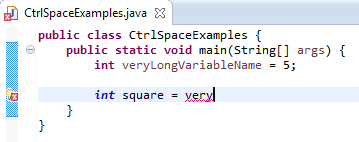
\includegraphics{ctrlspace_1.png}\hfill}

Wystarczy, że przy kolejnym użyciu wpiszesz fragment nazwy i wciśniesz Ctrl+Spacja, a długa nazwa zostanie uzupełniona:

{\hfill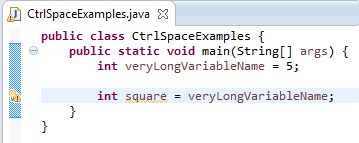
\includegraphics{ctrlspace_2.png}\hfill}

W początkowej fazie nauki Javy równie często wykorzystuje się instrukcję \emph{System.out.println()} - jej wpisywanie również można uprościć. Wystarczy, że wpiszesz \emph{syso} i wciśniesz Ctrl+Spację, a reszta zostanie uzupełniona.

{\hfill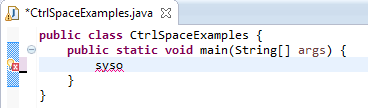
\includegraphics{syso_1.png}\hfill}

{\hfill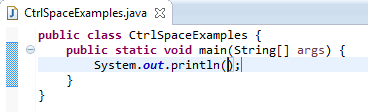
\includegraphics{syso_2.png}\hfill}


\subsubsection{CTRL + 1}
\label{wprowadzenie:ctrl-1}
Skrót, który przydaje się szczególnie wtedy, gdy dużo pracujemy na klawiaturze i nie przepadamy za sięganiem po mysz. Jeżeli przykładowo widzisz ostrzeżenie (podkreślenie na żółto) wystarczy, że najedziesz w dany obszar kursorem i wciśniesz Ctrl+1 a eclipse podpowie Ci sugerowane rozwiązania.

{\hfill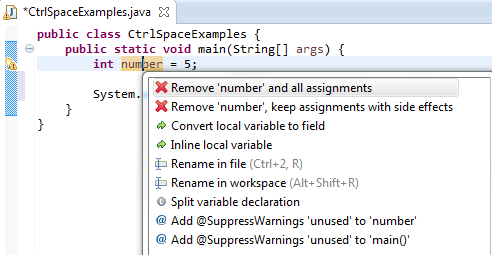
\includegraphics{number_1.png}\hfill}

W powyższym przykładzie widzimy ostrzeżenie, któe informuje nas o tym, że utworzyliśmy zmienną, której nigdzie nie wykorzystujemy - w podpowiedziach pojawia się m.in. możliwość jej usunięcia.


\subsubsection{Alt + Shift + R}
\label{wprowadzenie:alt-shift-r}
Jeżeli w swoim kodzie chcesz zmienić nazwę zmiennej lub zauważyłeś błąd typu literówka, to poprawienie tego może być problematyczne, ponieważ zmiennej tej prawdopodobnie używasz co najmniej w kilku innych miejscach. Wciskając skrót Ctrl+Shift+R na nazwie zmiennej, czy też nazwie klasy, możesz zmienić ich nazwę, a eclipse zadba o to, aby zaktualizować jej nazwę również we wszystkich innych jej wystąpieniach w kodzie źródłowym.

{\hfill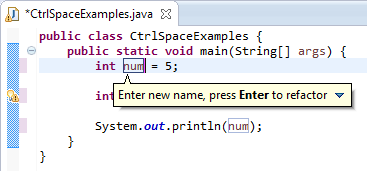
\includegraphics{refactor.png}\hfill}


\section{Programowanie obiektowe}
\label{obiekty:programowanie-obiektowe}\label{obiekty:centrum-edukacji-obywatelskiej}\label{obiekty::doc}
\textbf{Czego się dowiesz}
\begin{itemize}
\item {} 
Czym jest programowanie obiektowe

\item {} 
Jaka jest różnica między klasą a obiektem

\item {} 
W jaki sposób definiować własne typy danych

\item {} 
Czym są metody i konstruktory

\item {} 
Czym jest przeciążanie metod i konstruktorów

\item {} 
Do czego służy słowo kluczowe

\item {} 
Czym są pakiety i jakie są możliwe specyfikatory dostępu

\item {} 
Jak porównywać obiekty

\end{itemize}

\textbf{Czym jest programowanie obiektowe?}

Czysto teoretycznie programowaniem obiektowym najłatwiej nazwać próbę odwzorowania bytów ze świata rzeczywistego w naszej aplikacji poprzez utworzenie nowych, bardziej złożonych typów danych.

Dużo prościej jest to jednak zrozumieć na konkretnych przykładach, do których za chwilę przejdziemy.


\subsection{Klasy i obiekty}
\label{obiekty:klasy-i-obiekty}
\textbf{Ćwiczenie}
Wyobraź sobie, że tworzysz aplikację prostą aplikację do obsługi sklepu komputerowego. Najważniejsze będzie w niej zdecydowanie przechowywanie informacji o produktach. Wypisz kilka cech produktu, które Twoim zdaniem będą istotne z punktu widzenia użytkownika tej aplikacji(sprzedawcy).

Przykłady cech przydatnych

\begin{Verbatim}[commandchars=\\\{\}]
Nazwa produktu
Cena
Producent
Model / nazwa kodowa
Rok produkcji
\end{Verbatim}

Możliwe, że rzeczy, które wypisałeś są inne od pokazanych powyżej - to bardzo dobrze! Świadczyć to może o różnej wizji na aplikację. Na tę chwilę ograniczymy się do dwóch podstawowych informacji, czyli nazwy produktu oraz jego ceny. Te dwie podstawowe rzeczy na dobrą sprawę pozwolą nam znaleźć dowolny towar w bazie wszystkich produktów oraz dokonać sprzedaży na podstawie podanej ceny.

\textbf{Ćwiczenie} \emph{(5 min)}
\begin{quote}

Napisz prosty program, w którym w zmiennych przechowasz informacje o 2 różnych produktach (np. Monitor Samsung Syncmaster za 700zł oraz Laptop HP Probook 450 za 3000zł). Wydrukuj następnie informacje o tych produktach na ekranie. Wykorzystaj różne typy danych do przechowywania nazw produktów a inne do przechowywania ceny.
\end{quote}

\emph{plik Shop.java}

\begin{Verbatim}[commandchars=\\\{\},numbers=left,firstnumber=1,stepnumber=1]
\PYG{k+kd}{public} \PYG{k+kd}{class} \PYG{n+nc}{Shop} \PYG{o}{\PYGZob{}}
    \PYG{k+kd}{public} \PYG{k+kd}{static} \PYG{k+kt}{void} \PYG{n+nf}{main}\PYG{o}{(}\PYG{n}{String}\PYG{o}{[}\PYG{o}{]} \PYG{n}{args}\PYG{o}{)} \PYG{o}{\PYGZob{}}
        \PYG{n}{String} \PYG{n}{product1Name} \PYG{o}{=} \PYG{l+s}{\PYGZdq{}Samsung Syncmaster\PYGZdq{}}\PYG{o}{;}
        \PYG{k+kt}{double} \PYG{n}{product1Price} \PYG{o}{=} \PYG{l+m+mf}{700.0}\PYG{o}{;}

        \PYG{n}{String} \PYG{n}{product2Name} \PYG{o}{=} \PYG{l+s}{\PYGZdq{}HP Probook 450\PYGZdq{}}\PYG{o}{;}
        \PYG{k+kt}{double} \PYG{n}{product2Price} \PYG{o}{=} \PYG{l+m+mf}{3000.0}\PYG{o}{;}

        \PYG{n}{System}\PYG{o}{.}\PYG{n+na}{out}\PYG{o}{.}\PYG{n+na}{println}\PYG{o}{(}\PYG{l+s}{\PYGZdq{}Produkty w sklepie: \PYGZdq{}}\PYG{o}{)}\PYG{o}{;}
        \PYG{n}{System}\PYG{o}{.}\PYG{n+na}{out}\PYG{o}{.}\PYG{n+na}{println}\PYG{o}{(}\PYG{n}{product1Name} \PYG{o}{+} \PYG{l+s}{\PYGZdq{}:\PYGZdq{}} \PYG{o}{+} \PYG{n}{product1Price}\PYG{o}{)}\PYG{o}{;}
        \PYG{n}{System}\PYG{o}{.}\PYG{n+na}{out}\PYG{o}{.}\PYG{n+na}{println}\PYG{o}{(}\PYG{n}{product2Name} \PYG{o}{+} \PYG{l+s}{\PYGZdq{}: \PYGZdq{}} \PYG{o}{+} \PYG{n}{product2Price}\PYG{o}{)}\PYG{o}{;}
    \PYG{o}{\PYGZcb{}}
\PYG{o}{\PYGZcb{}}
\end{Verbatim}

Wszystko wygląda na pierwszy rzut oka w porządku, ale zastanów się teraz w jaki sposób zapisałbyś informację o kilkuset produktach w tym sklepie? Możliwe, że przychodzi Ci do głowy utworzenie tablic z imionami, nazwiskami itd. Nie jest to najgorszy pomysł, jednak ma jedną dużą wadę - dane nie są spójne i w żaden sposób ze sobą powiązane. Zmiana czegokolwiek, np dodanie 1 produktu, wiązałoby się z koniecznością aktualizacji innej tablicy z cenami, należałoby uważać na odwoływanie się do odpowiednich indeksów tablic itd.

Tutaj dochodzimy do sedna programowania obiektowego. Czy nie byłoby świetną sprawą możliwość utworzenia swojego typu danych ``Product'', który moglibyśmy wykorzystywać tak jak wartości typu int, czy double? W Javie możemy zdefiniować swój typ, zwyczajnie tworząc nową klasę, a w niej definiując zmienne typów prostych (lub wcześniej utworzonych typów obiektowych).

\begin{notice}{note}{Note:}
Klasą nazywamy zbiór cech oraz funkcjonalności obiektu, który chcemy odwzorować w pamięci komputera.
\end{notice}

\emph{plik Product.java}

\begin{Verbatim}[commandchars=\\\{\},numbers=left,firstnumber=1,stepnumber=1]
\PYG{k+kd}{public} \PYG{k+kd}{class} \PYG{n+nc}{Product} \PYG{o}{\PYGZob{}}
    \PYG{n}{String} \PYG{n}{name}\PYG{o}{;}
    \PYG{k+kt}{double} \PYG{n}{price}\PYG{o}{;}
\PYG{o}{\PYGZcb{}}
\end{Verbatim}

Struktura projektu eclipse:

{\hfill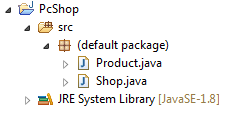
\includegraphics{pcshop_eclipse_1.png}\hfill}

Na podstawie takiej klasy możemy utworzyć \textbf{obiekt}. Obiekty zawsze będziemy tworzyli poprzez zapis \textbf{new NazwaKlasy();} przekazując w nawiasie ewentualne parametry (o tym za chwilę).

\begin{notice}{note}{Note:}
Obiektem nazywamy konkretny egzemplarz danej klasy. Klasą nazwiemy ``Produkt'', ale obiektem '' produkt laptop HP Probook 450 kosztujący 3000zł''.
\end{notice}

\emph{plik Shop.java}

\begin{Verbatim}[commandchars=\\\{\},numbers=left,firstnumber=1,stepnumber=1]
\PYG{k+kd}{public} \PYG{k+kd}{class} \PYG{n+nc}{Shop} \PYG{o}{\PYGZob{}}
    \PYG{k+kd}{public} \PYG{k+kd}{static} \PYG{k+kt}{void} \PYG{n+nf}{main}\PYG{o}{(}\PYG{n}{String}\PYG{o}{[}\PYG{o}{]} \PYG{n}{args}\PYG{o}{)} \PYG{o}{\PYGZob{}}
        \PYG{n}{Product} \PYG{n}{product1} \PYG{o}{=} \PYG{k}{new} \PYG{n}{Product}\PYG{o}{(}\PYG{o}{)}\PYG{o}{;}
        \PYG{n}{product1}\PYG{o}{.}\PYG{n+na}{name} \PYG{o}{=} \PYG{l+s}{\PYGZdq{}Samsung Syncmaster\PYGZdq{}}\PYG{o}{;}
        \PYG{n}{product1}\PYG{o}{.}\PYG{n+na}{price} \PYG{o}{=} \PYG{l+m+mf}{700.0}\PYG{o}{;}

        \PYG{n}{Product} \PYG{n}{product2} \PYG{o}{=} \PYG{k}{new} \PYG{n}{Product}\PYG{o}{(}\PYG{o}{)}\PYG{o}{;}
        \PYG{n}{product2}\PYG{o}{.}\PYG{n+na}{name} \PYG{o}{=} \PYG{l+s}{\PYGZdq{}HP Probook 450\PYGZdq{}}\PYG{o}{;}
        \PYG{n}{product2}\PYG{o}{.}\PYG{n+na}{price} \PYG{o}{=} \PYG{l+m+mf}{3000.0}\PYG{o}{;}

        \PYG{n}{System}\PYG{o}{.}\PYG{n+na}{out}\PYG{o}{.}\PYG{n+na}{println}\PYG{o}{(}\PYG{l+s}{\PYGZdq{}Produkty w sklepie: \PYGZdq{}}\PYG{o}{)}\PYG{o}{;}
        \PYG{n}{System}\PYG{o}{.}\PYG{n+na}{out}\PYG{o}{.}\PYG{n+na}{println}\PYG{o}{(}\PYG{n}{product1}\PYG{o}{.}\PYG{n+na}{name} \PYG{o}{+} \PYG{l+s}{\PYGZdq{}:\PYGZdq{}} \PYG{o}{+} \PYG{n}{product1}\PYG{o}{.}\PYG{n+na}{price}\PYG{o}{)}\PYG{o}{;}
        \PYG{n}{System}\PYG{o}{.}\PYG{n+na}{out}\PYG{o}{.}\PYG{n+na}{println}\PYG{o}{(}\PYG{n}{product2}\PYG{o}{.}\PYG{n+na}{name} \PYG{o}{+} \PYG{l+s}{\PYGZdq{}: \PYGZdq{}} \PYG{o}{+} \PYG{n}{product2}\PYG{o}{.}\PYG{n+na}{price}\PYG{o}{)}\PYG{o}{;}
    \PYG{o}{\PYGZcb{}}
\PYG{o}{\PYGZcb{}}
\end{Verbatim}

Jak widzisz zmienne \emph{name} i \emph{price} z wcześniejszego kodu są teraz opakowane w \textbf{obiekty} typu Product. Do poszczególnych \textbf{pól klasy} odwołujemy się za pomocą operatora kropki, np. \emph{``product1.name''}.

\begin{notice}{note}{Note:}
Jeżeli nie zainicjujesz poszczególnych klas obiektu, przyjmą one wartości domyślne. Dla typów liczbowych jest to 0 lub 0.0, dla typu char specjalna wartość pusta, a dla typów obiektowych (w tym String) jest to wartość null.
\end{notice}

\begin{notice}{attention}{Attention:}
Często powtarzającym się błędem w Javie jest {\color{red}\bfseries{}**}NullPointerException*. Oznacza on, że obiekt, do którego próbujesz się odwołać nie został utworzony, a jedynie zadeklarowany. Jeżeli zobaczysz go w eclipse sprawdż więc, czy przypisałeś do odpowiedniej zmiennej (referencji) obiekt utworzony za pomocą słowa new.
\end{notice}

Na chwilę obecną może Ci się wydawać, że zrobiło się tylko więcej kodu, a program nadal robi to samo. Zwróć jednak uwagę, że dane są teraz bardziej spójne, a dzięki podejściu obiektowemu informacje o np. 100 produktach możemy przechowywać w tylko 1 tablicy typu \emph{Product{[}{]}}.

\emph{plik Shop.java}

\begin{Verbatim}[commandchars=\\\{\},numbers=left,firstnumber=1,stepnumber=1]
\PYG{k+kd}{public} \PYG{k+kd}{class} \PYG{n+nc}{Shop} \PYG{o}{\PYGZob{}}
    \PYG{k+kd}{public} \PYG{k+kd}{static} \PYG{k+kt}{void} \PYG{n+nf}{main}\PYG{o}{(}\PYG{n}{String}\PYG{o}{[}\PYG{o}{]} \PYG{n}{args}\PYG{o}{)} \PYG{o}{\PYGZob{}}
        \PYG{n}{Product}\PYG{o}{[}\PYG{o}{]} \PYG{n}{products} \PYG{o}{=} \PYG{k}{new} \PYG{n}{Product}\PYG{o}{[}\PYG{l+m+mi}{2}\PYG{o}{]}\PYG{o}{;}

        \PYG{n}{products}\PYG{o}{[}\PYG{l+m+mi}{0}\PYG{o}{]} \PYG{o}{=} \PYG{k}{new} \PYG{n}{Product}\PYG{o}{(}\PYG{o}{)}\PYG{o}{;}
        \PYG{n}{products}\PYG{o}{[}\PYG{l+m+mi}{0}\PYG{o}{]}\PYG{o}{.}\PYG{n+na}{name} \PYG{o}{=} \PYG{l+s}{\PYGZdq{}Samsung Syncmaster\PYGZdq{}}\PYG{o}{;}
        \PYG{n}{products}\PYG{o}{[}\PYG{l+m+mi}{0}\PYG{o}{]}\PYG{o}{.}\PYG{n+na}{price} \PYG{o}{=} \PYG{l+m+mf}{700.0}\PYG{o}{;}

        \PYG{n}{products}\PYG{o}{[}\PYG{l+m+mi}{1}\PYG{o}{]} \PYG{o}{=} \PYG{k}{new} \PYG{n}{Product}\PYG{o}{(}\PYG{o}{)}\PYG{o}{;}
        \PYG{n}{products}\PYG{o}{[}\PYG{l+m+mi}{1}\PYG{o}{]}\PYG{o}{.}\PYG{n+na}{name} \PYG{o}{=} \PYG{l+s}{\PYGZdq{}HP Probook 450\PYGZdq{}}\PYG{o}{;}
        \PYG{n}{products}\PYG{o}{[}\PYG{l+m+mi}{1}\PYG{o}{]}\PYG{o}{.}\PYG{n+na}{price} \PYG{o}{=} \PYG{l+m+mf}{3000.0}\PYG{o}{;}

        \PYG{n}{System}\PYG{o}{.}\PYG{n+na}{out}\PYG{o}{.}\PYG{n+na}{println}\PYG{o}{(}\PYG{l+s}{\PYGZdq{}Produkty w sklepie: \PYGZdq{}}\PYG{o}{)}\PYG{o}{;}
        \PYG{n}{System}\PYG{o}{.}\PYG{n+na}{out}\PYG{o}{.}\PYG{n+na}{println}\PYG{o}{(}\PYG{n}{products}\PYG{o}{[}\PYG{l+m+mi}{0}\PYG{o}{]}\PYG{o}{.}\PYG{n+na}{name} \PYG{o}{+} \PYG{l+s}{\PYGZdq{}:\PYGZdq{}} \PYG{o}{+} \PYG{n}{products}\PYG{o}{[}\PYG{l+m+mi}{0}\PYG{o}{]}\PYG{o}{.}\PYG{n+na}{price}\PYG{o}{)}\PYG{o}{;}
        \PYG{n}{System}\PYG{o}{.}\PYG{n+na}{out}\PYG{o}{.}\PYG{n+na}{println}\PYG{o}{(}\PYG{n}{products}\PYG{o}{[}\PYG{l+m+mi}{1}\PYG{o}{]}\PYG{o}{.}\PYG{n+na}{name} \PYG{o}{+} \PYG{l+s}{\PYGZdq{}: \PYGZdq{}} \PYG{o}{+} \PYG{n}{products}\PYG{o}{[}\PYG{l+m+mi}{1}\PYG{o}{]}\PYG{o}{.}\PYG{n+na}{price}\PYG{o}{)}\PYG{o}{;}
    \PYG{o}{\PYGZcb{}}
\PYG{o}{\PYGZcb{}}
\end{Verbatim}

\textbf{Ćwiczenie} \emph{(10 min)}
\begin{quote}

Wyobraź sobie, że tworzysz aplikację do diagnostyki komputerowej samochodów. Zacznij od utworzenia klasy Car przechowującej informacje o marce producenta, modelu, roku produkcji i mocy silnika. W drugiej klasie o nazwie CarDiagnostic utwórz dwa obiekty klasy Car i wyświetl informacje o samochodach na ekranie.
\end{quote}

Struktura projektu:

{\hfill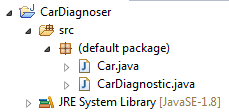
\includegraphics{car_project1.png}\hfill}

\emph{plik Car.java}

\begin{Verbatim}[commandchars=\\\{\},numbers=left,firstnumber=1,stepnumber=1]
\PYG{k+kd}{public} \PYG{k+kd}{class} \PYG{n+nc}{Car} \PYG{o}{\PYGZob{}}
    \PYG{n}{String} \PYG{n}{carBrand}\PYG{o}{;} \PYG{c+c1}{// marka samochodu}
    \PYG{n}{String} \PYG{n}{model}\PYG{o}{;}
    \PYG{k+kt}{int} \PYG{n}{year}\PYG{o}{;} \PYG{c+c1}{//rok produkcji}
    \PYG{k+kt}{int} \PYG{n}{horsePower}\PYG{o}{;} \PYG{c+c1}{// ilość koni mechanicznych}
\PYG{o}{\PYGZcb{}}
\end{Verbatim}

\emph{plik CarDiagnostic.java}

\begin{Verbatim}[commandchars=\\\{\},numbers=left,firstnumber=1,stepnumber=1]
\PYG{k+kd}{public} \PYG{k+kd}{class} \PYG{n+nc}{CarDiagnostic} \PYG{o}{\PYGZob{}}
    \PYG{k+kd}{public} \PYG{k+kd}{static} \PYG{k+kt}{void} \PYG{n+nf}{main}\PYG{o}{(}\PYG{n}{String}\PYG{o}{[}\PYG{o}{]} \PYG{n}{args}\PYG{o}{)} \PYG{o}{\PYGZob{}}
        \PYG{n}{Car} \PYG{n}{audiA4} \PYG{o}{=} \PYG{k}{new} \PYG{n}{Car}\PYG{o}{(}\PYG{o}{)}\PYG{o}{;}
        \PYG{n}{audiA4}\PYG{o}{.}\PYG{n+na}{carBrand} \PYG{o}{=} \PYG{l+s}{\PYGZdq{}Audi\PYGZdq{}}\PYG{o}{;}
        \PYG{n}{audiA4}\PYG{o}{.}\PYG{n+na}{model} \PYG{o}{=} \PYG{l+s}{\PYGZdq{}A4\PYGZdq{}}\PYG{o}{;}
        \PYG{n}{audiA4}\PYG{o}{.}\PYG{n+na}{year} \PYG{o}{=} \PYG{l+m+mi}{2008}\PYG{o}{;}
        \PYG{n}{audiA4}\PYG{o}{.}\PYG{n+na}{horsePower} \PYG{o}{=} \PYG{l+m+mi}{170}\PYG{o}{;}

        \PYG{n}{Car} \PYG{n}{vwGolf} \PYG{o}{=} \PYG{k}{new} \PYG{n}{Car}\PYG{o}{(}\PYG{o}{)}\PYG{o}{;}
        \PYG{n}{vwGolf}\PYG{o}{.}\PYG{n+na}{carBrand} \PYG{o}{=} \PYG{l+s}{\PYGZdq{}Volkswagen\PYGZdq{}}\PYG{o}{;}
        \PYG{n}{vwGolf}\PYG{o}{.}\PYG{n+na}{model} \PYG{o}{=} \PYG{l+s}{\PYGZdq{}Golf\PYGZdq{}}\PYG{o}{;}
        \PYG{n}{vwGolf}\PYG{o}{.}\PYG{n+na}{year} \PYG{o}{=} \PYG{l+m+mi}{2010}\PYG{o}{;}
        \PYG{n}{vwGolf}\PYG{o}{.}\PYG{n+na}{horsePower} \PYG{o}{=} \PYG{l+m+mi}{130}\PYG{o}{;}

        \PYG{n}{System}\PYG{o}{.}\PYG{n+na}{out}\PYG{o}{.}\PYG{n+na}{println}\PYG{o}{(}\PYG{l+s}{\PYGZdq{}Samochód 1: \PYGZdq{}}\PYG{o}{)}\PYG{o}{;}
        \PYG{n}{System}\PYG{o}{.}\PYG{n+na}{out}\PYG{o}{.}\PYG{n+na}{println}\PYG{o}{(}\PYG{n}{audiA4}\PYG{o}{.}\PYG{n+na}{carBrand} \PYG{o}{+} \PYG{l+s}{\PYGZdq{} \PYGZdq{}} \PYG{o}{+} \PYG{n}{audiA4}\PYG{o}{.}\PYG{n+na}{model}
                \PYG{o}{+} \PYG{l+s}{\PYGZdq{}, rok produkcji: \PYGZdq{}} \PYG{o}{+} \PYG{n}{audiA4}\PYG{o}{.}\PYG{n+na}{year} \PYG{o}{+} \PYG{l+s}{\PYGZdq{}, moc: \PYGZdq{}}
                \PYG{o}{+} \PYG{n}{audiA4}\PYG{o}{.}\PYG{n+na}{horsePower}\PYG{o}{)}\PYG{o}{;}

        \PYG{n}{System}\PYG{o}{.}\PYG{n+na}{out}\PYG{o}{.}\PYG{n+na}{println}\PYG{o}{(}\PYG{l+s}{\PYGZdq{}Samochód 2: \PYGZdq{}}\PYG{o}{)}\PYG{o}{;}
        \PYG{n}{System}\PYG{o}{.}\PYG{n+na}{out}\PYG{o}{.}\PYG{n+na}{println}\PYG{o}{(}\PYG{n}{vwGolf}\PYG{o}{.}\PYG{n+na}{carBrand} \PYG{o}{+} \PYG{l+s}{\PYGZdq{} \PYGZdq{}} \PYG{o}{+} \PYG{n}{vwGolf}\PYG{o}{.}\PYG{n+na}{model}
                \PYG{o}{+} \PYG{l+s}{\PYGZdq{}, rok produkcji: \PYGZdq{}} \PYG{o}{+} \PYG{n}{vwGolf}\PYG{o}{.}\PYG{n+na}{year} \PYG{o}{+} \PYG{l+s}{\PYGZdq{}, moc: \PYGZdq{}}
                \PYG{o}{+} \PYG{n}{vwGolf}\PYG{o}{.}\PYG{n+na}{horsePower}\PYG{o}{)}\PYG{o}{;}
    \PYG{o}{\PYGZcb{}}
\PYG{o}{\PYGZcb{}}
\end{Verbatim}


\subsection{Metody}
\label{obiekty:metody}
Klasa Product potrafi już przechowywać informacje o nazwie i cenie produktu, jednak jak wspomnieliśmy w definicji klasy jest to także zbiór funkcjonalności. W programowaniu obiektowym funkcjonalności danej klasy realizuje się poprzez utworzenie \textbf{metod}. W naszym przykładzie funkcjonalnością może być na przykład zwrócenie przez obiekt klasy Product nazwy oraz ceny w czytelnej formie, dzięki czemu w metodzie println() nie będziemy musieli się odwoływać do poszczególnych pól.

\emph{plik Product.java}

\begin{Verbatim}[commandchars=\\\{\},numbers=left,firstnumber=1,stepnumber=1]
\PYG{k+kd}{public} \PYG{k+kd}{class} \PYG{n+nc}{Product} \PYG{o}{\PYGZob{}}
    \PYG{n}{String} \PYG{n}{name}\PYG{o}{;}
    \PYG{k+kt}{double} \PYG{n}{price}\PYG{o}{;}

    \PYG{n}{String} \PYG{n+nf}{getProductInfo}\PYG{o}{(}\PYG{o}{)} \PYG{o}{\PYGZob{}}
        \PYG{k}{return} \PYG{n}{name} \PYG{o}{+} \PYG{l+s}{\PYGZdq{}: \PYGZdq{}} \PYG{o}{+} \PYG{n}{price}\PYG{o}{;}
    \PYG{o}{\PYGZcb{}}
\PYG{o}{\PYGZcb{}}
\end{Verbatim}

W klasie Product utworzyliśmy metodę \textbf{getProductInfo}. Ponieważ zwraca ona opisową formę produktu musieliśmy zadeklarować jej typ jako String. Wynik metody należy zwrócić za pomocą słowa kluczowego \textbf{return}.

\begin{notice}{note}{Note:}
Ogólna postać metody to:

\begin{Verbatim}[commandchars=\\\{\}]
typ\PYGZus{}zwracany nazwaMetody(opcjonalne\PYGZus{}argumenty\PYGZus{}metody) \PYGZob{}
  //ciało metody między nawiasami klamrowymi
\PYGZcb{}
\end{Verbatim}

Elementami opcjonalnymi są jeszcze specyfikatory dostępu (np. public) oraz oznaczenie metody jako statycznej (static) - do tego dojdziemy jednak niebawem. Metody mogą zwracać wynik (np. String) i wtedy musi w nich występować instrukcja \textbf{return}, ale mogą także nie zwracać żadnego wyniku - sytuacja taka będzie miała miejsce, gdy metoda ma za zadanie np. wydrukować coś na ekranie za pomocą System.out.print(). Jeżeli metoda nie zwraca żadnego wyniku należy jako jej typ zwracany podać słowo kluczowe \textbf{void}. Przykładem metody, która nie zwraca żadnego wyniku jest metoda \textbf{main}, którą poznałeś już na samym początku kursu.
\end{notice}

\emph{plik Shop.java}

\begin{Verbatim}[commandchars=\\\{\},numbers=left,firstnumber=1,stepnumber=1]
\PYG{k+kd}{public} \PYG{k+kd}{class} \PYG{n+nc}{Shop} \PYG{o}{\PYGZob{}}
    \PYG{k+kd}{public} \PYG{k+kd}{static} \PYG{k+kt}{void} \PYG{n+nf}{main}\PYG{o}{(}\PYG{n}{String}\PYG{o}{[}\PYG{o}{]} \PYG{n}{args}\PYG{o}{)} \PYG{o}{\PYGZob{}}
        \PYG{n}{Product}\PYG{o}{[}\PYG{o}{]} \PYG{n}{products} \PYG{o}{=} \PYG{k}{new} \PYG{n}{Product}\PYG{o}{[}\PYG{l+m+mi}{2}\PYG{o}{]}\PYG{o}{;}

        \PYG{n}{products}\PYG{o}{[}\PYG{l+m+mi}{0}\PYG{o}{]} \PYG{o}{=} \PYG{k}{new} \PYG{n}{Product}\PYG{o}{(}\PYG{o}{)}\PYG{o}{;}
        \PYG{n}{products}\PYG{o}{[}\PYG{l+m+mi}{0}\PYG{o}{]}\PYG{o}{.}\PYG{n+na}{name} \PYG{o}{=} \PYG{l+s}{\PYGZdq{}Samsung Syncmaster\PYGZdq{}}\PYG{o}{;}
        \PYG{n}{products}\PYG{o}{[}\PYG{l+m+mi}{0}\PYG{o}{]}\PYG{o}{.}\PYG{n+na}{price} \PYG{o}{=} \PYG{l+m+mf}{700.0}\PYG{o}{;}

        \PYG{n}{products}\PYG{o}{[}\PYG{l+m+mi}{1}\PYG{o}{]} \PYG{o}{=} \PYG{k}{new} \PYG{n}{Product}\PYG{o}{(}\PYG{o}{)}\PYG{o}{;}
        \PYG{n}{products}\PYG{o}{[}\PYG{l+m+mi}{1}\PYG{o}{]}\PYG{o}{.}\PYG{n+na}{name} \PYG{o}{=} \PYG{l+s}{\PYGZdq{}HP Probook 450\PYGZdq{}}\PYG{o}{;}
        \PYG{n}{products}\PYG{o}{[}\PYG{l+m+mi}{1}\PYG{o}{]}\PYG{o}{.}\PYG{n+na}{price} \PYG{o}{=} \PYG{l+m+mf}{3000.0}\PYG{o}{;}

        \PYG{n}{System}\PYG{o}{.}\PYG{n+na}{out}\PYG{o}{.}\PYG{n+na}{println}\PYG{o}{(}\PYG{l+s}{\PYGZdq{}Produkty w sklepie: \PYGZdq{}}\PYG{o}{)}\PYG{o}{;}
        \PYG{n}{System}\PYG{o}{.}\PYG{n+na}{out}\PYG{o}{.}\PYG{n+na}{println}\PYG{o}{(}\PYG{n}{products}\PYG{o}{[}\PYG{l+m+mi}{0}\PYG{o}{]}\PYG{o}{.}\PYG{n+na}{getProductInfo}\PYG{o}{(}\PYG{o}{)}\PYG{o}{)}\PYG{o}{;}
        \PYG{n}{System}\PYG{o}{.}\PYG{n+na}{out}\PYG{o}{.}\PYG{n+na}{println}\PYG{o}{(}\PYG{n}{products}\PYG{o}{[}\PYG{l+m+mi}{1}\PYG{o}{]}\PYG{o}{.}\PYG{n+na}{getProductInfo}\PYG{o}{(}\PYG{o}{)}\PYG{o}{)}\PYG{o}{;}
    \PYG{o}{\PYGZcb{}}
\PYG{o}{\PYGZcb{}}
\end{Verbatim}


\subsection{Konstruktory}
\label{obiekty:konstruktory}
Ostatnią rzeczą, którą możemy uprościć w klasie Shop jest inicjalizacja zmiennych. W chwili obecnej w celu utworzenia jednego tylko obiektu potrzebujemy aż 3 linijek kodu - w przypadku tworzenia 100 obiektów, kod rozrasta się do 300 linii - jest to niedopuszczalne.

Tworzenie obiektów możemy jednak uprościć za pomocą specjalnych metod nazywanych \textbf{konstruktorami}.

\begin{notice}{note}{Note:}
Konstruktor to specjalna metoda, która nie ma zadeklarowanego żadnego zwracanego typu (nawet void), a jej nazwa jest identyczna z nazwą klasy, w której się znajduje (z uwzględnieniem wielkości liter). Podobnie jak każda inna metoda może przyjmować argumenty.
\end{notice}

\emph{plik Product.java}

\begin{Verbatim}[commandchars=\\\{\},numbers=left,firstnumber=1,stepnumber=1]
\PYG{k+kd}{public} \PYG{k+kd}{class} \PYG{n+nc}{Product} \PYG{o}{\PYGZob{}}
    \PYG{n}{String} \PYG{n}{name}\PYG{o}{;}
    \PYG{k+kt}{double} \PYG{n}{price}\PYG{o}{;}

    \PYG{c+c1}{//konstruktor przyjmujący 2 argumenty}
    \PYG{n}{Product}\PYG{o}{(}\PYG{n}{String} \PYG{n}{n}\PYG{o}{,} \PYG{k+kt}{double} \PYG{n}{p}\PYG{o}{)} \PYG{o}{\PYGZob{}}
        \PYG{n}{name} \PYG{o}{=} \PYG{n}{n}\PYG{o}{;}
        \PYG{n}{price} \PYG{o}{=} \PYG{n}{p}\PYG{o}{;}
    \PYG{o}{\PYGZcb{}}

    \PYG{n}{String} \PYG{n+nf}{getProductInfo}\PYG{o}{(}\PYG{o}{)} \PYG{o}{\PYGZob{}}
        \PYG{k}{return} \PYG{n}{name} \PYG{o}{+} \PYG{l+s}{\PYGZdq{}: \PYGZdq{}} \PYG{o}{+} \PYG{n}{price}\PYG{o}{;}
    \PYG{o}{\PYGZcb{}}
\PYG{o}{\PYGZcb{}}
\end{Verbatim}

Nasz konstruktor przyjmuje dwa argumenty - jeden typu String, a drugi typu double. Wartości przekazane jako argumenty konstruktora przypisujemy następnie do pól klasy, czyli \emph{name} oraz \emph{price}. Teraz możemy uprościć tworzenie obiektów w klasie Shop do tylko jednej linijki dla każdego z nich:

\emph{plik Shop.java}

\begin{Verbatim}[commandchars=\\\{\},numbers=left,firstnumber=1,stepnumber=1]
\PYG{k+kd}{public} \PYG{k+kd}{class} \PYG{n+nc}{Shop} \PYG{o}{\PYGZob{}}
    \PYG{k+kd}{public} \PYG{k+kd}{static} \PYG{k+kt}{void} \PYG{n+nf}{main}\PYG{o}{(}\PYG{n}{String}\PYG{o}{[}\PYG{o}{]} \PYG{n}{args}\PYG{o}{)} \PYG{o}{\PYGZob{}}
        \PYG{n}{Product}\PYG{o}{[}\PYG{o}{]} \PYG{n}{products} \PYG{o}{=} \PYG{k}{new} \PYG{n}{Product}\PYG{o}{[}\PYG{l+m+mi}{2}\PYG{o}{]}\PYG{o}{;}

        \PYG{n}{products}\PYG{o}{[}\PYG{l+m+mi}{0}\PYG{o}{]} \PYG{o}{=} \PYG{k}{new} \PYG{n}{Product}\PYG{o}{(}\PYG{l+s}{\PYGZdq{}Samsung Syncmaster\PYGZdq{}}\PYG{o}{,} \PYG{l+m+mf}{700.0}\PYG{o}{)}\PYG{o}{;}

        \PYG{n}{products}\PYG{o}{[}\PYG{l+m+mi}{1}\PYG{o}{]} \PYG{o}{=} \PYG{k}{new} \PYG{n}{Product}\PYG{o}{(}\PYG{l+s}{\PYGZdq{}HP Probook 450\PYGZdq{}}\PYG{o}{,} \PYG{l+m+mf}{3000.0}\PYG{o}{)}\PYG{o}{;}

        \PYG{n}{System}\PYG{o}{.}\PYG{n+na}{out}\PYG{o}{.}\PYG{n+na}{println}\PYG{o}{(}\PYG{l+s}{\PYGZdq{}Produkty w sklepie: \PYGZdq{}}\PYG{o}{)}\PYG{o}{;}
        \PYG{n}{System}\PYG{o}{.}\PYG{n+na}{out}\PYG{o}{.}\PYG{n+na}{println}\PYG{o}{(}\PYG{n}{products}\PYG{o}{[}\PYG{l+m+mi}{0}\PYG{o}{]}\PYG{o}{.}\PYG{n+na}{getProductInfo}\PYG{o}{(}\PYG{o}{)}\PYG{o}{)}\PYG{o}{;}
        \PYG{n}{System}\PYG{o}{.}\PYG{n+na}{out}\PYG{o}{.}\PYG{n+na}{println}\PYG{o}{(}\PYG{n}{products}\PYG{o}{[}\PYG{l+m+mi}{1}\PYG{o}{]}\PYG{o}{.}\PYG{n+na}{getProductInfo}\PYG{o}{(}\PYG{o}{)}\PYG{o}{)}\PYG{o}{;}
    \PYG{o}{\PYGZcb{}}
\PYG{o}{\PYGZcb{}}
\end{Verbatim}

\begin{notice}{attention}{Attention:}
Każda klasa posiada domyślnie jeden niejawny konstruktor (bez parametrów). Jeżeli jednak zdefiniujesz w swojej klasie chociaż jeden konstruktor przyjmujący dowolne argumenty, to konstruktor domyślny przestaje istnieć.
\end{notice}

\textbf{Ćwiczenie} \emph{(10 min)}
\begin{quote}

Rozwiń aplikację z poprzedniego ćwiczenia (diagnostyka sanmochodu) o następujące informacje. W klasie Car dodaj konstruktor pozwalający zainicjować wszystkie pola klasy oraz dwie metody: getInfo(), która zwróci opisową formę danego samochodu, a także upgreade(), która zwiększa moc silnika o tyle koni mechanicznych ile przekażemy jako jej parametr. Przetestuj nowe funkcjonalności w klasie CarDiagnostic.
\end{quote}

\emph{plik Car.java}

\begin{Verbatim}[commandchars=\\\{\},numbers=left,firstnumber=1,stepnumber=1]
\PYG{k+kd}{public} \PYG{k+kd}{class} \PYG{n+nc}{Car} \PYG{o}{\PYGZob{}}

    \PYG{n}{String} \PYG{n}{carBrand}\PYG{o}{;} \PYG{c+c1}{// marka samochodu}
    \PYG{n}{String} \PYG{n}{model}\PYG{o}{;}
    \PYG{k+kt}{int} \PYG{n}{year}\PYG{o}{;} \PYG{c+c1}{//rok produkcji}
    \PYG{k+kt}{int} \PYG{n}{horsePower}\PYG{o}{;} \PYG{c+c1}{// ilość koni mechanicznych}

    \PYG{c+c1}{//konstruktor do zainicjowania wszystkich pól}
    \PYG{n}{Car}\PYG{o}{(}\PYG{n}{String} \PYG{n}{cb}\PYG{o}{,} \PYG{n}{String} \PYG{n}{m}\PYG{o}{,} \PYG{k+kt}{int} \PYG{n}{y}\PYG{o}{,} \PYG{k+kt}{int} \PYG{n}{hp}\PYG{o}{)} \PYG{o}{\PYGZob{}}
        \PYG{n}{carBrand} \PYG{o}{=} \PYG{n}{cb}\PYG{o}{;}
        \PYG{n}{model} \PYG{o}{=} \PYG{n}{m}\PYG{o}{;}
        \PYG{n}{year} \PYG{o}{=} \PYG{n}{y}\PYG{o}{;}
        \PYG{n}{horsePower} \PYG{o}{=} \PYG{n}{hp}\PYG{o}{;}
    \PYG{o}{\PYGZcb{}}

    \PYG{c+c1}{//zwiększenie mocy silnika}
    \PYG{k+kt}{void} \PYG{n+nf}{upgreade}\PYG{o}{(}\PYG{k+kt}{int} \PYG{n}{hp}\PYG{o}{)} \PYG{o}{\PYGZob{}}
        \PYG{n}{horsePower} \PYG{o}{=} \PYG{n}{horsePower} \PYG{o}{+} \PYG{n}{hp}\PYG{o}{;}
    \PYG{o}{\PYGZcb{}}

    \PYG{c+c1}{//zwrócenie opisowej formy samochodu}
    \PYG{n}{String} \PYG{n+nf}{getInfo}\PYG{o}{(}\PYG{o}{)} \PYG{o}{\PYGZob{}}
        \PYG{k}{return} \PYG{n}{carBrand} \PYG{o}{+} \PYG{l+s}{\PYGZdq{} \PYGZdq{}} \PYG{o}{+} \PYG{n}{model} \PYG{o}{+} \PYG{l+s}{\PYGZdq{}; \PYGZdq{}} \PYG{o}{+} \PYG{n}{year} \PYG{o}{+} \PYG{l+s}{\PYGZdq{}; \PYGZdq{}} \PYG{o}{+} \PYG{n}{horsePower} \PYG{o}{+} \PYG{l+s}{\PYGZdq{}HP\PYGZdq{}}\PYG{o}{;}
    \PYG{o}{\PYGZcb{}}
\PYG{o}{\PYGZcb{}}
\end{Verbatim}

\emph{plik CarDiagnostic.java}

\begin{Verbatim}[commandchars=\\\{\},numbers=left,firstnumber=1,stepnumber=1]
\PYG{k+kd}{public} \PYG{k+kd}{class} \PYG{n+nc}{CarDiagnostic} \PYG{o}{\PYGZob{}}
    \PYG{k+kd}{public} \PYG{k+kd}{static} \PYG{k+kt}{void} \PYG{n+nf}{main}\PYG{o}{(}\PYG{n}{String}\PYG{o}{[}\PYG{o}{]} \PYG{n}{args}\PYG{o}{)} \PYG{o}{\PYGZob{}}
        \PYG{c+c1}{//utworzenie obiektów}
        \PYG{n}{Car} \PYG{n}{audiA4} \PYG{o}{=} \PYG{k}{new} \PYG{n}{Car}\PYG{o}{(}\PYG{l+s}{\PYGZdq{}Audi\PYGZdq{}}\PYG{o}{,} \PYG{l+s}{\PYGZdq{}A4\PYGZdq{}}\PYG{o}{,} \PYG{l+m+mi}{2008}\PYG{o}{,} \PYG{l+m+mi}{170}\PYG{o}{)}\PYG{o}{;}
        \PYG{n}{Car} \PYG{n}{vwGolf} \PYG{o}{=} \PYG{k}{new} \PYG{n}{Car}\PYG{o}{(}\PYG{l+s}{\PYGZdq{}Volkswagen\PYGZdq{}}\PYG{o}{,} \PYG{l+s}{\PYGZdq{}Golf\PYGZdq{}}\PYG{o}{,} \PYG{l+m+mi}{2010}\PYG{o}{,} \PYG{l+m+mi}{130}\PYG{o}{)}\PYG{o}{;}

        \PYG{c+c1}{//tuning}
        \PYG{n}{audiA4}\PYG{o}{.}\PYG{n+na}{upgreade}\PYG{o}{(}\PYG{l+m+mi}{30}\PYG{o}{)}\PYG{o}{;}
        \PYG{n}{vwGolf}\PYG{o}{.}\PYG{n+na}{upgreade}\PYG{o}{(}\PYG{l+m+mi}{20}\PYG{o}{)}\PYG{o}{;}

        \PYG{c+c1}{//wydruk informacji}
        \PYG{n}{System}\PYG{o}{.}\PYG{n+na}{out}\PYG{o}{.}\PYG{n+na}{println}\PYG{o}{(}\PYG{l+s}{\PYGZdq{}Samochód 1: \PYGZdq{}}\PYG{o}{)}\PYG{o}{;}
        \PYG{n}{System}\PYG{o}{.}\PYG{n+na}{out}\PYG{o}{.}\PYG{n+na}{println}\PYG{o}{(}\PYG{n}{audiA4}\PYG{o}{.}\PYG{n+na}{getInfo}\PYG{o}{(}\PYG{o}{)}\PYG{o}{)}\PYG{o}{;}

        \PYG{n}{System}\PYG{o}{.}\PYG{n+na}{out}\PYG{o}{.}\PYG{n+na}{println}\PYG{o}{(}\PYG{l+s}{\PYGZdq{}Samochód 2: \PYGZdq{}}\PYG{o}{)}\PYG{o}{;}
        \PYG{n}{System}\PYG{o}{.}\PYG{n+na}{out}\PYG{o}{.}\PYG{n+na}{println}\PYG{o}{(}\PYG{n}{vwGolf}\PYG{o}{.}\PYG{n+na}{getInfo}\PYG{o}{(}\PYG{o}{)}\PYG{o}{)}\PYG{o}{;}
    \PYG{o}{\PYGZcb{}}
\PYG{o}{\PYGZcb{}}
\end{Verbatim}


\subsection{Przeciążanie metod i konstruktorów}
\label{obiekty:przeciazanie-metod-i-konstruktorow}
Czasami może zdarzyć się sytuacja, w której nie będziemy mieli pełnych informacji o danym produkcie, który chcielibyśmy utworzyć. Przykładowo będziemy mieli jego nazwę, ale będziemy musieli jeszcze chwilę poczekać na ustalenie jej ceny w centrali. W takiej sytuacji możemy utworzyć kilka konstruktorów, które pozwolą nam zainicjować obiekt danej klasy. Gdy w klasie istnieje kilka konstruktorów lub metod o takiej samej nazwie, ale różniących się przyjmowanymi parametrami, to będziemy mówili o nich, że są dostępne w kilku \textbf{przeciążonych} wersjach.

\emph{plik Product.java}

\begin{Verbatim}[commandchars=\\\{\},numbers=left,firstnumber=1,stepnumber=1]
\PYG{k+kd}{public} \PYG{k+kd}{class} \PYG{n+nc}{Product} \PYG{o}{\PYGZob{}}
    \PYG{n}{String} \PYG{n}{name}\PYG{o}{;}
    \PYG{k+kt}{double} \PYG{n}{price}\PYG{o}{;}

    \PYG{c+c1}{//konstruktory}
    \PYG{n}{Product}\PYG{o}{(}\PYG{n}{String} \PYG{n}{n}\PYG{o}{,} \PYG{k+kt}{double} \PYG{n}{p}\PYG{o}{)} \PYG{o}{\PYGZob{}}
        \PYG{n}{name} \PYG{o}{=} \PYG{n}{n}\PYG{o}{;}
        \PYG{n}{price} \PYG{o}{=} \PYG{n}{p}\PYG{o}{;}
    \PYG{o}{\PYGZcb{}}

    \PYG{n}{Product}\PYG{o}{(}\PYG{n}{String} \PYG{n}{n}\PYG{o}{)} \PYG{o}{\PYGZob{}}
        \PYG{n}{name} \PYG{o}{=} \PYG{n}{n}\PYG{o}{;}
    \PYG{o}{\PYGZcb{}}

    \PYG{n}{String} \PYG{n+nf}{getProductInfo}\PYG{o}{(}\PYG{o}{)} \PYG{o}{\PYGZob{}}
        \PYG{k}{return} \PYG{n}{name} \PYG{o}{+} \PYG{l+s}{\PYGZdq{}: \PYGZdq{}} \PYG{o}{+} \PYG{n}{price}\PYG{o}{;}
    \PYG{o}{\PYGZcb{}}
\PYG{o}{\PYGZcb{}}
\end{Verbatim}

W powyższym przykładzie widzimy, że utworzyliśmy drugi konstruktor, który inicjuje jedynie nazwę produktu. Cena (price) przyjmie w takiej sytuacji wartość domyślną, którą dla typu double jest 0.0. W podobny sposób możemy przeciążać dowolne metody, które będą miały takie same nazwy, ale przyjmą różne parametry.

\textbf{Ćwiczenie} \emph{(5 min)}
\begin{quote}

W programie do diagnostyki samochodu dopisz dodatkowy konstruktor pozwoli zainicjować jedynie markę i model samochodu, pozostawiając rok produkcji i moc silnika wartościami domyślnymi. W klasie CarDiagnostic utwórz za pomocą tego konstruktora nowy obiekt i wyświetl informacje o nim na ekranie.
\end{quote}

\emph{plik Car.java}

\begin{Verbatim}[commandchars=\\\{\},numbers=left,firstnumber=1,stepnumber=1]
\PYG{k+kd}{public} \PYG{k+kd}{class} \PYG{n+nc}{Car} \PYG{o}{\PYGZob{}}

    \PYG{n}{String} \PYG{n}{carBrand}\PYG{o}{;} \PYG{c+c1}{// marka samochodu}
    \PYG{n}{String} \PYG{n}{model}\PYG{o}{;}
    \PYG{k+kt}{int} \PYG{n}{year}\PYG{o}{;} \PYG{c+c1}{//rok produkcji}
    \PYG{k+kt}{int} \PYG{n}{horsePower}\PYG{o}{;} \PYG{c+c1}{// ilość koni mechanicznych}

    \PYG{n}{Car}\PYG{o}{(}\PYG{n}{String} \PYG{n}{cb}\PYG{o}{,} \PYG{n}{String} \PYG{n}{m}\PYG{o}{)} \PYG{o}{\PYGZob{}}
        \PYG{n}{carBrand} \PYG{o}{=} \PYG{n}{cb}\PYG{o}{;}
        \PYG{n}{model} \PYG{o}{=} \PYG{n}{m}\PYG{o}{;}
    \PYG{o}{\PYGZcb{}}

    \PYG{n}{Car}\PYG{o}{(}\PYG{n}{String} \PYG{n}{cb}\PYG{o}{,} \PYG{n}{String} \PYG{n}{m}\PYG{o}{,} \PYG{k+kt}{int} \PYG{n}{y}\PYG{o}{,} \PYG{k+kt}{int} \PYG{n}{hp}\PYG{o}{)} \PYG{o}{\PYGZob{}}
        \PYG{n}{carBrand} \PYG{o}{=} \PYG{n}{cb}\PYG{o}{;}
        \PYG{n}{model} \PYG{o}{=} \PYG{n}{m}\PYG{o}{;}
        \PYG{n}{year} \PYG{o}{=} \PYG{n}{y}\PYG{o}{;}
        \PYG{n}{horsePower} \PYG{o}{=} \PYG{n}{hp}\PYG{o}{;}
    \PYG{o}{\PYGZcb{}}

    \PYG{k+kt}{void} \PYG{n+nf}{upgreade}\PYG{o}{(}\PYG{k+kt}{int} \PYG{n}{hp}\PYG{o}{)} \PYG{o}{\PYGZob{}}
        \PYG{n}{horsePower} \PYG{o}{=} \PYG{n}{horsePower} \PYG{o}{+} \PYG{n}{hp}\PYG{o}{;}
    \PYG{o}{\PYGZcb{}}

    \PYG{n}{String} \PYG{n+nf}{getInfo}\PYG{o}{(}\PYG{o}{)} \PYG{o}{\PYGZob{}}
        \PYG{k}{return} \PYG{n}{carBrand} \PYG{o}{+} \PYG{l+s}{\PYGZdq{} \PYGZdq{}} \PYG{o}{+} \PYG{n}{model} \PYG{o}{+} \PYG{l+s}{\PYGZdq{}; \PYGZdq{}} \PYG{o}{+} \PYG{n}{year} \PYG{o}{+} \PYG{l+s}{\PYGZdq{}; \PYGZdq{}} \PYG{o}{+} \PYG{n}{horsePower} \PYG{o}{+} \PYG{l+s}{\PYGZdq{}HP\PYGZdq{}}\PYG{o}{;}
    \PYG{o}{\PYGZcb{}}
\PYG{o}{\PYGZcb{}}
\end{Verbatim}

\emph{plik CarDiagnostic.java}

\begin{Verbatim}[commandchars=\\\{\},numbers=left,firstnumber=1,stepnumber=1]
\PYG{k+kd}{public} \PYG{k+kd}{class} \PYG{n+nc}{CarDiagnostic} \PYG{o}{\PYGZob{}}
    \PYG{k+kd}{public} \PYG{k+kd}{static} \PYG{k+kt}{void} \PYG{n+nf}{main}\PYG{o}{(}\PYG{n}{String}\PYG{o}{[}\PYG{o}{]} \PYG{n}{args}\PYG{o}{)} \PYG{o}{\PYGZob{}}
        \PYG{n}{Car} \PYG{n}{audiA4} \PYG{o}{=} \PYG{k}{new} \PYG{n}{Car}\PYG{o}{(}\PYG{l+s}{\PYGZdq{}Audi\PYGZdq{}}\PYG{o}{,} \PYG{l+s}{\PYGZdq{}A4\PYGZdq{}}\PYG{o}{,} \PYG{l+m+mi}{2008}\PYG{o}{,} \PYG{l+m+mi}{170}\PYG{o}{)}\PYG{o}{;}
        \PYG{n}{Car} \PYG{n}{vwGolf} \PYG{o}{=} \PYG{k}{new} \PYG{n}{Car}\PYG{o}{(}\PYG{l+s}{\PYGZdq{}Volkswagen\PYGZdq{}}\PYG{o}{,} \PYG{l+s}{\PYGZdq{}Golf\PYGZdq{}}\PYG{o}{,} \PYG{l+m+mi}{2010}\PYG{o}{,} \PYG{l+m+mi}{130}\PYG{o}{)}\PYG{o}{;}
        \PYG{n}{Car} \PYG{n}{opelCorsa} \PYG{o}{=} \PYG{k}{new} \PYG{n}{Car}\PYG{o}{(}\PYG{l+s}{\PYGZdq{}Opel\PYGZdq{}}\PYG{o}{,} \PYG{l+s}{\PYGZdq{}Corsa\PYGZdq{}}\PYG{o}{)}\PYG{o}{;}

        \PYG{c+c1}{//tuning}
        \PYG{n}{audiA4}\PYG{o}{.}\PYG{n+na}{upgreade}\PYG{o}{(}\PYG{l+m+mi}{30}\PYG{o}{)}\PYG{o}{;}
        \PYG{n}{vwGolf}\PYG{o}{.}\PYG{n+na}{upgreade}\PYG{o}{(}\PYG{l+m+mi}{20}\PYG{o}{)}\PYG{o}{;}

        \PYG{n}{System}\PYG{o}{.}\PYG{n+na}{out}\PYG{o}{.}\PYG{n+na}{println}\PYG{o}{(}\PYG{l+s}{\PYGZdq{}Samochód 1: \PYGZdq{}}\PYG{o}{)}\PYG{o}{;}
        \PYG{n}{System}\PYG{o}{.}\PYG{n+na}{out}\PYG{o}{.}\PYG{n+na}{println}\PYG{o}{(}\PYG{n}{audiA4}\PYG{o}{.}\PYG{n+na}{getInfo}\PYG{o}{(}\PYG{o}{)}\PYG{o}{)}\PYG{o}{;}

        \PYG{n}{System}\PYG{o}{.}\PYG{n+na}{out}\PYG{o}{.}\PYG{n+na}{println}\PYG{o}{(}\PYG{l+s}{\PYGZdq{}Samochód 2: \PYGZdq{}}\PYG{o}{)}\PYG{o}{;}
        \PYG{n}{System}\PYG{o}{.}\PYG{n+na}{out}\PYG{o}{.}\PYG{n+na}{println}\PYG{o}{(}\PYG{n}{vwGolf}\PYG{o}{.}\PYG{n+na}{getInfo}\PYG{o}{(}\PYG{o}{)}\PYG{o}{)}\PYG{o}{;}

        \PYG{n}{System}\PYG{o}{.}\PYG{n+na}{out}\PYG{o}{.}\PYG{n+na}{println}\PYG{o}{(}\PYG{l+s}{\PYGZdq{}Samochód 3: \PYGZdq{}}\PYG{o}{)}\PYG{o}{;}
        \PYG{n}{System}\PYG{o}{.}\PYG{n+na}{out}\PYG{o}{.}\PYG{n+na}{println}\PYG{o}{(}\PYG{n}{opelCorsa}\PYG{o}{.}\PYG{n+na}{getInfo}\PYG{o}{(}\PYG{o}{)}\PYG{o}{)}\PYG{o}{;}
    \PYG{o}{\PYGZcb{}}
\PYG{o}{\PYGZcb{}}
\end{Verbatim}


\subsection{Słowo kluczowe this}
\label{obiekty:slowo-kluczowe-this}
Zarówno aplikacja symulująca sklep z częściami komputerowymi jak i program symulujący diagnostykę samochodową posiadają już pewną bazową funkcjonalność. Czytelność kodu w kilku miejscach można jednak poprawić.

Dobrą praktyką jest stosowanie wszędzie tam gdzie to możliwe opisowych nazw zmiennych, jednak w naszym przypadku ciężko wymyślić zamiennik dla ``name'', czy ``year'' (stosowanie polskich nazw również nie jest dobrą praktyką). Na szczęście przewidziano również taką funkcjonalność języka i nazwy argumentów metod, czy konstruktorów mogą być identyczne z nazwami pól klasy, te drugie należy jednak poprzedzić dodatkowo słowem kluczowym \textbf{this}.

Tym sposobem nasza poprawiona klasa Product prezentuje się jak poniżej.

\emph{plik Product.java}

\begin{Verbatim}[commandchars=\\\{\},numbers=left,firstnumber=1,stepnumber=1]
\PYG{k+kd}{public} \PYG{k+kd}{class} \PYG{n+nc}{Product} \PYG{o}{\PYGZob{}}
    \PYG{n}{String} \PYG{n}{name}\PYG{o}{;}
    \PYG{k+kt}{double} \PYG{n}{price}\PYG{o}{;}

    \PYG{c+c1}{//konstruktory}
    \PYG{n}{Product}\PYG{o}{(}\PYG{n}{String} \PYG{n}{name}\PYG{o}{,} \PYG{k+kt}{double} \PYG{n}{price}\PYG{o}{)} \PYG{o}{\PYGZob{}}
        \PYG{k}{this}\PYG{o}{.}\PYG{n+na}{name} \PYG{o}{=} \PYG{n}{name}\PYG{o}{;}
        \PYG{k}{this}\PYG{o}{.}\PYG{n+na}{price} \PYG{o}{=} \PYG{n}{price}\PYG{o}{;}
    \PYG{o}{\PYGZcb{}}

    \PYG{n}{Product}\PYG{o}{(}\PYG{n}{String} \PYG{n}{name}\PYG{o}{)} \PYG{o}{\PYGZob{}}
        \PYG{k}{this}\PYG{o}{.}\PYG{n+na}{name} \PYG{o}{=} \PYG{n}{name}\PYG{o}{;}
    \PYG{o}{\PYGZcb{}}

    \PYG{n}{String} \PYG{n+nf}{getProductInfo}\PYG{o}{(}\PYG{o}{)} \PYG{o}{\PYGZob{}}
        \PYG{k}{return} \PYG{n}{name} \PYG{o}{+} \PYG{l+s}{\PYGZdq{}: \PYGZdq{}} \PYG{o}{+} \PYG{n}{price}\PYG{o}{;}
    \PYG{o}{\PYGZcb{}}
\PYG{o}{\PYGZcb{}}
\end{Verbatim}

Zapis \emph{this.name = name} należy rozumieć jako ``przypisz do pola tej (this) klasy o nazwie \emph{name} wartość argumentu konstruktora o nazwie \emph{name}''.

Słowo kluczowe this ma także drugie zastosowanie, które pozwala wywoływać przeciążoną wersję konstruktora w innym konstruktorze. Ma to takie zastosowanie, że pozwala zaoszczędzić powtarzalnego kodu w przypadku, gdy w klasie zdefiniujemy np. 4 podobne konstruktory, w których spora część kodu źródłowego się powtarza. U nas nie zaoszczędzimy specjalnie kodu, jednak wygląda to następująco:

\emph{plik Product.java}

\begin{Verbatim}[commandchars=\\\{\},numbers=left,firstnumber=1,stepnumber=1]
\PYG{k+kd}{public} \PYG{k+kd}{class} \PYG{n+nc}{Product} \PYG{o}{\PYGZob{}}
    \PYG{n}{String} \PYG{n}{name}\PYG{o}{;}
    \PYG{k+kt}{double} \PYG{n}{price}\PYG{o}{;}

    \PYG{c+c1}{//konstruktory}
    \PYG{n}{Product}\PYG{o}{(}\PYG{n}{String} \PYG{n}{name}\PYG{o}{,} \PYG{k+kt}{double} \PYG{n}{price}\PYG{o}{)} \PYG{o}{\PYGZob{}}
        \PYG{k}{this}\PYG{o}{(}\PYG{n}{name}\PYG{o}{)}\PYG{o}{;} \PYG{c+c1}{//wywołanie innego konstruktora}
        \PYG{k}{this}\PYG{o}{.}\PYG{n+na}{price} \PYG{o}{=} \PYG{n}{price}\PYG{o}{;}
    \PYG{o}{\PYGZcb{}}

    \PYG{n}{Product}\PYG{o}{(}\PYG{n}{String} \PYG{n}{name}\PYG{o}{)} \PYG{o}{\PYGZob{}}
        \PYG{k}{this}\PYG{o}{.}\PYG{n+na}{name} \PYG{o}{=} \PYG{n}{name}\PYG{o}{;}
    \PYG{o}{\PYGZcb{}}

    \PYG{n}{String} \PYG{n+nf}{getProductInfo}\PYG{o}{(}\PYG{o}{)} \PYG{o}{\PYGZob{}}
        \PYG{k}{return} \PYG{n}{name} \PYG{o}{+} \PYG{l+s}{\PYGZdq{}: \PYGZdq{}} \PYG{o}{+} \PYG{n}{price}\PYG{o}{;}
    \PYG{o}{\PYGZcb{}}
\PYG{o}{\PYGZcb{}}
\end{Verbatim}

Jak widzisz w konstruktorze przyjmującym dwa argumenty wywołujemy w pierwszej kolejności konstruktor z jednym argumentem poprzez this(name). W ten sposób zainicjowaliśmy pole name, a następnie możemy zainicjować cenę, czyli pole price.

\textbf{Ćwiczenie} \emph{(5 min)}
\begin{quote}

Popraw klasę Car z poprzedniego zadania w taki sposób, aby nazwy argumentów konstruktorów miały bardziej znaczące nazwy (najlepiej takie same jak nazwy pól klasy). Wykorzystaj także słowo kluczowe this w celu wywołania w jednym z konstruktorów drugiego konstruktora i zaoszczędzić tym samym powtarzalnego kodu.
\end{quote}

\emph{plik Car.java}

\begin{Verbatim}[commandchars=\\\{\},numbers=left,firstnumber=1,stepnumber=1]
\PYG{k+kd}{public} \PYG{k+kd}{class} \PYG{n+nc}{Car} \PYG{o}{\PYGZob{}}

    \PYG{n}{String} \PYG{n}{carBrand}\PYG{o}{;} \PYG{c+c1}{// marka samochodu}
    \PYG{n}{String} \PYG{n}{model}\PYG{o}{;}
    \PYG{k+kt}{int} \PYG{n}{year}\PYG{o}{;} \PYG{c+c1}{//rok produkcji}
    \PYG{k+kt}{int} \PYG{n}{horsePower}\PYG{o}{;} \PYG{c+c1}{// ilość koni mechanicznych}

    \PYG{n}{Car}\PYG{o}{(}\PYG{n}{String} \PYG{n}{carBrand}\PYG{o}{,} \PYG{n}{String} \PYG{n}{model}\PYG{o}{)} \PYG{o}{\PYGZob{}}
        \PYG{k}{this}\PYG{o}{.}\PYG{n+na}{carBrand} \PYG{o}{=} \PYG{n}{carBrand}\PYG{o}{;}
        \PYG{k}{this}\PYG{o}{.}\PYG{n+na}{model} \PYG{o}{=} \PYG{n}{model}\PYG{o}{;}
    \PYG{o}{\PYGZcb{}}

    \PYG{n}{Car}\PYG{o}{(}\PYG{n}{String} \PYG{n}{carBrand}\PYG{o}{,} \PYG{n}{String} \PYG{n}{model}\PYG{o}{,} \PYG{k+kt}{int} \PYG{n}{year}\PYG{o}{,} \PYG{k+kt}{int} \PYG{n}{horsePower}\PYG{o}{)} \PYG{o}{\PYGZob{}}
        \PYG{k}{this}\PYG{o}{(}\PYG{n}{carBrand}\PYG{o}{,} \PYG{n}{model}\PYG{o}{)}\PYG{o}{;}
        \PYG{k}{this}\PYG{o}{.}\PYG{n+na}{year} \PYG{o}{=} \PYG{n}{year}\PYG{o}{;}
        \PYG{k}{this}\PYG{o}{.}\PYG{n+na}{horsePower} \PYG{o}{=} \PYG{n}{horsePower}\PYG{o}{;}
    \PYG{o}{\PYGZcb{}}

    \PYG{k+kt}{void} \PYG{n+nf}{upgreade}\PYG{o}{(}\PYG{k+kt}{int} \PYG{n}{hp}\PYG{o}{)} \PYG{o}{\PYGZob{}}
        \PYG{n}{horsePower} \PYG{o}{=} \PYG{n}{horsePower} \PYG{o}{+} \PYG{n}{hp}\PYG{o}{;}
    \PYG{o}{\PYGZcb{}}

    \PYG{n}{String} \PYG{n+nf}{getInfo}\PYG{o}{(}\PYG{o}{)} \PYG{o}{\PYGZob{}}
        \PYG{k}{return} \PYG{n}{carBrand} \PYG{o}{+} \PYG{l+s}{\PYGZdq{} \PYGZdq{}} \PYG{o}{+} \PYG{n}{model} \PYG{o}{+} \PYG{l+s}{\PYGZdq{}; \PYGZdq{}} \PYG{o}{+} \PYG{n}{year} \PYG{o}{+} \PYG{l+s}{\PYGZdq{}; \PYGZdq{}} \PYG{o}{+} \PYG{n}{horsePower} \PYG{o}{+} \PYG{l+s}{\PYGZdq{}HP\PYGZdq{}}\PYG{o}{;}
    \PYG{o}{\PYGZcb{}}
\PYG{o}{\PYGZcb{}}
\end{Verbatim}


\subsection{Pakiety i modyfikatory dostępu}
\label{obiekty:pakiety-i-modyfikatory-dostepu}
Istotnym elementem, który pomaga w organizacji większych projektów jest podział klas i plików źródłowych na pakiety. Pakiety są niczym innym jak dodatkowymi folderami, które pozwalają grupować wspólnie klasy, które odpowiadają za podobne funkcjonalności. W celu utworzenia pakietu wybieramy po prostu New -\textgreater{} Package. Nazewnictwo pakietów zazwyczaj odzwierciedla nazwę domeny autorów, czyli np. pl.org.ceo.kursjava.pakiet1 - gdzie pakiet1 powinien być jakąś znaczącą nazwą, kursjava nazwą projektu, a pl.org.ceo to odwrócona nazwa domeny Centrum Edukacji Obywatelskiej.

Gdy w kodzie projektu CarDiagnoser podzielimy klasy na dwa pakiety (przeciągnij klasy do odpowiednich pakietów:

{\hfill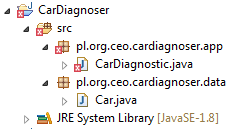
\includegraphics{package.png}\hfill}

zauważamy błąd w klasie CarDiagnostic.
\begin{quote}

package pl.org.ceo.cardiagnoser.app;
import pl.org.ceo.cardiagnoser.data.Car;

public class CarDiagnostic \{
//kod bez zmian
\}
\end{quote}

Pierwszą rzeczą, na którą warto zwrócić uwagę są dwiue linie kodu, które eclipse dodał automatycznie:
\begin{itemize}
\item {} 
package oznacza pakiet, w którym umieszczona jest dana klasa

\item {} 
import jest dyrektywą niezbędną w przypadku, gdy korzystamy z klas umieszczonych w innych pakietach. W naszym przypadku musieliśmy zaimportować klasę Car.

\end{itemize}

Błąd w klasie polega na tym, że konstruktor jest niewidoczny:

{\hfill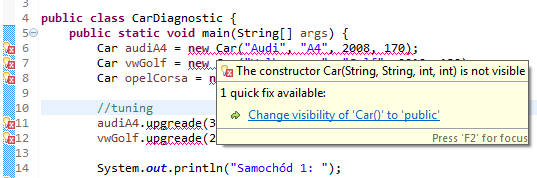
\includegraphics{constructor.png}\hfill}

Można sobie zadać pytanie, ale jak to niewidoczny, skoro przed chwilą z niego korzystaliśmy? Jest to spowodowane różnymi zasięgami widoczności pól metod i konstruktorów. W Javie istnieją cztery możliwe zasięgi:
\begin{itemize}
\item {} 
default - domyślny, czyli pakietowy zasięg dostępu

\item {} 
public - publiczny, można się odwoływać z dowolnego miejsca w pakiecie i poza nim

\item {} 
protected - zasięg ograniczony do danego pakietu

\item {} 
private - zasięg tylko w ramach jednej klasy. Do tak oznaczonych pól, metod i konstruktorów nie można odwołać się nawet z klas w tym samym pakiecie

\end{itemize}

Ponieważ klasy Car i CarDiagnoser znajdują się w różnych pakietach odpowiednie konstruktory i pola musimy oznaczyć jako publiczne:

\emph{plik Car.java}

\begin{Verbatim}[commandchars=\\\{\},numbers=left,firstnumber=1,stepnumber=1]
\PYG{k+kn}{package} \PYG{n}{pl}\PYG{o}{.}\PYG{n+na}{org}\PYG{o}{.}\PYG{n+na}{ceo}\PYG{o}{.}\PYG{n+na}{cardiagnoser}\PYG{o}{.}\PYG{n+na}{data}\PYG{o}{;}

\PYG{k+kd}{public} \PYG{k+kd}{class} \PYG{n+nc}{Car} \PYG{o}{\PYGZob{}}

    \PYG{k+kd}{public} \PYG{n}{String} \PYG{n}{carBrand}\PYG{o}{;} \PYG{c+c1}{// marka samochodu}
    \PYG{k+kd}{public} \PYG{n}{String} \PYG{n}{model}\PYG{o}{;}
    \PYG{k+kd}{public} \PYG{k+kt}{int} \PYG{n}{year}\PYG{o}{;} \PYG{c+c1}{//rok produkcji}
    \PYG{k+kd}{public} \PYG{k+kt}{int} \PYG{n}{horsePower}\PYG{o}{;} \PYG{c+c1}{// ilość koni mechanicznych}

    \PYG{k+kd}{public} \PYG{n+nf}{Car}\PYG{o}{(}\PYG{n}{String} \PYG{n}{carBrand}\PYG{o}{,} \PYG{n}{String} \PYG{n}{model}\PYG{o}{)} \PYG{o}{\PYGZob{}}
        \PYG{k}{this}\PYG{o}{.}\PYG{n+na}{carBrand} \PYG{o}{=} \PYG{n}{carBrand}\PYG{o}{;}
        \PYG{k}{this}\PYG{o}{.}\PYG{n+na}{model} \PYG{o}{=} \PYG{n}{model}\PYG{o}{;}
    \PYG{o}{\PYGZcb{}}

    \PYG{k+kd}{public} \PYG{n+nf}{Car}\PYG{o}{(}\PYG{n}{String} \PYG{n}{carBrand}\PYG{o}{,} \PYG{n}{String} \PYG{n}{model}\PYG{o}{,} \PYG{k+kt}{int} \PYG{n}{year}\PYG{o}{,} \PYG{k+kt}{int} \PYG{n}{horsePower}\PYG{o}{)} \PYG{o}{\PYGZob{}}
        \PYG{k}{this}\PYG{o}{(}\PYG{n}{carBrand}\PYG{o}{,} \PYG{n}{model}\PYG{o}{)}\PYG{o}{;}
        \PYG{k}{this}\PYG{o}{.}\PYG{n+na}{year} \PYG{o}{=} \PYG{n}{year}\PYG{o}{;}
        \PYG{k}{this}\PYG{o}{.}\PYG{n+na}{horsePower} \PYG{o}{=} \PYG{n}{horsePower}\PYG{o}{;}
    \PYG{o}{\PYGZcb{}}

    \PYG{k+kd}{public} \PYG{k+kt}{void} \PYG{n+nf}{upgreade}\PYG{o}{(}\PYG{k+kt}{int} \PYG{n}{hp}\PYG{o}{)} \PYG{o}{\PYGZob{}}
        \PYG{n}{horsePower} \PYG{o}{=} \PYG{n}{horsePower} \PYG{o}{+} \PYG{n}{hp}\PYG{o}{;}
    \PYG{o}{\PYGZcb{}}

    \PYG{k+kd}{public} \PYG{n}{String} \PYG{n+nf}{getInfo}\PYG{o}{(}\PYG{o}{)} \PYG{o}{\PYGZob{}}
        \PYG{k}{return} \PYG{n}{carBrand} \PYG{o}{+} \PYG{l+s}{\PYGZdq{} \PYGZdq{}} \PYG{o}{+} \PYG{n}{model} \PYG{o}{+} \PYG{l+s}{\PYGZdq{}; \PYGZdq{}} \PYG{o}{+} \PYG{n}{year} \PYG{o}{+} \PYG{l+s}{\PYGZdq{}; \PYGZdq{}} \PYG{o}{+} \PYG{n}{horsePower} \PYG{o}{+} \PYG{l+s}{\PYGZdq{}HP\PYGZdq{}}\PYG{o}{;}
    \PYG{o}{\PYGZcb{}}
\PYG{o}{\PYGZcb{}}
\end{Verbatim}

\begin{notice}{note}{Note:}
Nasze przykłady najczęściej będą na tyle proste, że dla uproszczenia wszystkie pliki będą znajdowały się w jednym pakiecie.
\end{notice}


\subsection{Porównywanie obiektów}
\label{obiekty:porownywanie-obiektow}
Ważnym zagadnieniem, które może sprawiać pewne problemy jest porównywanie obiektów w języku Java. Najważniejszym zagadnieniem jest tutaj zrozumienie tego, że obiekt i referencja wskazująca na ten obiekt (uproszczając - zmienna) to dwie różne rzeczy, któe porównujemy w różny sposób.

Obiekty zawsze powinniśmy porównywać za pomocą metody \textbf{equals()}. Jest to specjalna metoda, która jest dziedziczona przez każdą klasę Javy z klasy Object, która jest nadrzędną klasą dla wszystkich innych. Warto przesłonić metodę \emph{equals()} i zdefiniować w niej porównanie wszystkich pól klasy. Metodę \emph{equals()} możesz wygenerować w eclipse korzystając z opcji Source -\textgreater{} Generate hashCode() and equals(). Możemy następnie wybrać, któe pola muszą być równe, aby uznać, że dwa obiekty danego typu będą równe. Np. dla naszej wcześniejszej klasy Car wyglądałoby to następująco:

\emph{plik Car.java}

\begin{Verbatim}[commandchars=\\\{\},numbers=left,firstnumber=1,stepnumber=1]
\PYG{k+kn}{package} \PYG{n}{pl}\PYG{o}{.}\PYG{n+na}{org}\PYG{o}{.}\PYG{n+na}{ceo}\PYG{o}{.}\PYG{n+na}{cardiagnoser}\PYG{o}{.}\PYG{n+na}{data}\PYG{o}{;}

\PYG{k+kd}{public} \PYG{k+kd}{class} \PYG{n+nc}{Car} \PYG{o}{\PYGZob{}}

    \PYG{k+kd}{public} \PYG{n}{String} \PYG{n}{carBrand}\PYG{o}{;} \PYG{c+c1}{// marka samochodu}
    \PYG{k+kd}{public} \PYG{n}{String} \PYG{n}{model}\PYG{o}{;}
    \PYG{k+kd}{public} \PYG{k+kt}{int} \PYG{n}{year}\PYG{o}{;} \PYG{c+c1}{//rok produkcji}
    \PYG{k+kd}{public} \PYG{k+kt}{int} \PYG{n}{horsePower}\PYG{o}{;} \PYG{c+c1}{// ilość koni mechanicznych}

    \PYG{k+kd}{public} \PYG{n+nf}{Car}\PYG{o}{(}\PYG{n}{String} \PYG{n}{carBrand}\PYG{o}{,} \PYG{n}{String} \PYG{n}{model}\PYG{o}{)} \PYG{o}{\PYGZob{}}
        \PYG{k}{this}\PYG{o}{.}\PYG{n+na}{carBrand} \PYG{o}{=} \PYG{n}{carBrand}\PYG{o}{;}
        \PYG{k}{this}\PYG{o}{.}\PYG{n+na}{model} \PYG{o}{=} \PYG{n}{model}\PYG{o}{;}
    \PYG{o}{\PYGZcb{}}

    \PYG{k+kd}{public} \PYG{n+nf}{Car}\PYG{o}{(}\PYG{n}{String} \PYG{n}{carBrand}\PYG{o}{,} \PYG{n}{String} \PYG{n}{model}\PYG{o}{,} \PYG{k+kt}{int} \PYG{n}{year}\PYG{o}{,} \PYG{k+kt}{int} \PYG{n}{horsePower}\PYG{o}{)} \PYG{o}{\PYGZob{}}
        \PYG{k}{this}\PYG{o}{(}\PYG{n}{carBrand}\PYG{o}{,} \PYG{n}{model}\PYG{o}{)}\PYG{o}{;}
        \PYG{k}{this}\PYG{o}{.}\PYG{n+na}{year} \PYG{o}{=} \PYG{n}{year}\PYG{o}{;}
        \PYG{k}{this}\PYG{o}{.}\PYG{n+na}{horsePower} \PYG{o}{=} \PYG{n}{horsePower}\PYG{o}{;}
    \PYG{o}{\PYGZcb{}}

    \PYG{k+kd}{public} \PYG{k+kt}{void} \PYG{n+nf}{upgreade}\PYG{o}{(}\PYG{k+kt}{int} \PYG{n}{hp}\PYG{o}{)} \PYG{o}{\PYGZob{}}
        \PYG{n}{horsePower} \PYG{o}{=} \PYG{n}{horsePower} \PYG{o}{+} \PYG{n}{hp}\PYG{o}{;}
    \PYG{o}{\PYGZcb{}}

    \PYG{n+nd}{@Override}
    \PYG{k+kd}{public} \PYG{k+kt}{int} \PYG{n+nf}{hashCode}\PYG{o}{(}\PYG{o}{)} \PYG{o}{\PYGZob{}}
        \PYG{k+kd}{final} \PYG{k+kt}{int} \PYG{n}{prime} \PYG{o}{=} \PYG{l+m+mi}{31}\PYG{o}{;}
        \PYG{k+kt}{int} \PYG{n}{result} \PYG{o}{=} \PYG{l+m+mi}{1}\PYG{o}{;}
        \PYG{n}{result} \PYG{o}{=} \PYG{n}{prime} \PYG{o}{*} \PYG{n}{result}
                \PYG{o}{+} \PYG{o}{(}\PYG{o}{(}\PYG{n}{carBrand} \PYG{o}{=}\PYG{o}{=} \PYG{k+kc}{null}\PYG{o}{)} \PYG{o}{?} \PYG{l+m+mi}{0} \PYG{o}{:} \PYG{n}{carBrand}\PYG{o}{.}\PYG{n+na}{hashCode}\PYG{o}{(}\PYG{o}{)}\PYG{o}{)}\PYG{o}{;}
        \PYG{n}{result} \PYG{o}{=} \PYG{n}{prime} \PYG{o}{*} \PYG{n}{result} \PYG{o}{+} \PYG{n}{horsePower}\PYG{o}{;}
        \PYG{n}{result} \PYG{o}{=} \PYG{n}{prime} \PYG{o}{*} \PYG{n}{result} \PYG{o}{+} \PYG{o}{(}\PYG{o}{(}\PYG{n}{model} \PYG{o}{=}\PYG{o}{=} \PYG{k+kc}{null}\PYG{o}{)} \PYG{o}{?} \PYG{l+m+mi}{0} \PYG{o}{:} \PYG{n}{model}\PYG{o}{.}\PYG{n+na}{hashCode}\PYG{o}{(}\PYG{o}{)}\PYG{o}{)}\PYG{o}{;}
        \PYG{n}{result} \PYG{o}{=} \PYG{n}{prime} \PYG{o}{*} \PYG{n}{result} \PYG{o}{+} \PYG{n}{year}\PYG{o}{;}
        \PYG{k}{return} \PYG{n}{result}\PYG{o}{;}
    \PYG{o}{\PYGZcb{}}

    \PYG{n+nd}{@Override}
    \PYG{k+kd}{public} \PYG{k+kt}{boolean} \PYG{n+nf}{equals}\PYG{o}{(}\PYG{n}{Object} \PYG{n}{obj}\PYG{o}{)} \PYG{o}{\PYGZob{}}
        \PYG{k}{if} \PYG{o}{(}\PYG{k}{this} \PYG{o}{=}\PYG{o}{=} \PYG{n}{obj}\PYG{o}{)}
            \PYG{k}{return} \PYG{k+kc}{true}\PYG{o}{;}
        \PYG{k}{if} \PYG{o}{(}\PYG{n}{obj} \PYG{o}{=}\PYG{o}{=} \PYG{k+kc}{null}\PYG{o}{)}
            \PYG{k}{return} \PYG{k+kc}{false}\PYG{o}{;}
        \PYG{k}{if} \PYG{o}{(}\PYG{n}{getClass}\PYG{o}{(}\PYG{o}{)} \PYG{o}{!}\PYG{o}{=} \PYG{n}{obj}\PYG{o}{.}\PYG{n+na}{getClass}\PYG{o}{(}\PYG{o}{)}\PYG{o}{)}
            \PYG{k}{return} \PYG{k+kc}{false}\PYG{o}{;}
        \PYG{n}{Car} \PYG{n}{other} \PYG{o}{=} \PYG{o}{(}\PYG{n}{Car}\PYG{o}{)} \PYG{n}{obj}\PYG{o}{;}
        \PYG{k}{if} \PYG{o}{(}\PYG{n}{carBrand} \PYG{o}{=}\PYG{o}{=} \PYG{k+kc}{null}\PYG{o}{)} \PYG{o}{\PYGZob{}}
            \PYG{k}{if} \PYG{o}{(}\PYG{n}{other}\PYG{o}{.}\PYG{n+na}{carBrand} \PYG{o}{!}\PYG{o}{=} \PYG{k+kc}{null}\PYG{o}{)}
                \PYG{k}{return} \PYG{k+kc}{false}\PYG{o}{;}
        \PYG{o}{\PYGZcb{}} \PYG{k}{else} \PYG{k}{if} \PYG{o}{(}\PYG{o}{!}\PYG{n}{carBrand}\PYG{o}{.}\PYG{n+na}{equals}\PYG{o}{(}\PYG{n}{other}\PYG{o}{.}\PYG{n+na}{carBrand}\PYG{o}{)}\PYG{o}{)}
            \PYG{k}{return} \PYG{k+kc}{false}\PYG{o}{;}
        \PYG{k}{if} \PYG{o}{(}\PYG{n}{horsePower} \PYG{o}{!}\PYG{o}{=} \PYG{n}{other}\PYG{o}{.}\PYG{n+na}{horsePower}\PYG{o}{)}
            \PYG{k}{return} \PYG{k+kc}{false}\PYG{o}{;}
        \PYG{k}{if} \PYG{o}{(}\PYG{n}{model} \PYG{o}{=}\PYG{o}{=} \PYG{k+kc}{null}\PYG{o}{)} \PYG{o}{\PYGZob{}}
            \PYG{k}{if} \PYG{o}{(}\PYG{n}{other}\PYG{o}{.}\PYG{n+na}{model} \PYG{o}{!}\PYG{o}{=} \PYG{k+kc}{null}\PYG{o}{)}
                \PYG{k}{return} \PYG{k+kc}{false}\PYG{o}{;}
        \PYG{o}{\PYGZcb{}} \PYG{k}{else} \PYG{k}{if} \PYG{o}{(}\PYG{o}{!}\PYG{n}{model}\PYG{o}{.}\PYG{n+na}{equals}\PYG{o}{(}\PYG{n}{other}\PYG{o}{.}\PYG{n+na}{model}\PYG{o}{)}\PYG{o}{)}
            \PYG{k}{return} \PYG{k+kc}{false}\PYG{o}{;}
        \PYG{k}{if} \PYG{o}{(}\PYG{n}{year} \PYG{o}{!}\PYG{o}{=} \PYG{n}{other}\PYG{o}{.}\PYG{n+na}{year}\PYG{o}{)}
            \PYG{k}{return} \PYG{k+kc}{false}\PYG{o}{;}
        \PYG{k}{return} \PYG{k+kc}{true}\PYG{o}{;}
    \PYG{o}{\PYGZcb{}}

    \PYG{k+kd}{public} \PYG{n}{String} \PYG{n+nf}{getInfo}\PYG{o}{(}\PYG{o}{)} \PYG{o}{\PYGZob{}}
        \PYG{k}{return} \PYG{n}{carBrand} \PYG{o}{+} \PYG{l+s}{\PYGZdq{} \PYGZdq{}} \PYG{o}{+} \PYG{n}{model} \PYG{o}{+} \PYG{l+s}{\PYGZdq{}; \PYGZdq{}} \PYG{o}{+} \PYG{n}{year} \PYG{o}{+} \PYG{l+s}{\PYGZdq{}; \PYGZdq{}} \PYG{o}{+} \PYG{n}{horsePower} \PYG{o}{+} \PYG{l+s}{\PYGZdq{}HP\PYGZdq{}}\PYG{o}{;}
    \PYG{o}{\PYGZcb{}}
\PYG{o}{\PYGZcb{}}
\end{Verbatim}

Metoda hashCode() generowane wspólnie z equals() jest tzw. funkcją mieszającą i zwraca unikalny identyfikator obiektu obliczony na podstawie jego pól. Nie będziemy się w tym miejscu zagłębiali w jej zastosowanie, jednak należy pamiętać, że jeżeli metoda equals (porównanie dwóch obiektów) zwraca true, to wynik metody hashCode() dla tych dwóch obiektów także powinien być równy.

Teraz jeszcze w celu uzupełnienia wróćmy do kwestii porównania referencji vs porównania faktycznych obiektów. Jeżeli zapiszemy np.:

\begin{Verbatim}[commandchars=\\\{\}]
Car car1 = new Car(\PYGZdq{}VW\PYGZdq{}, \PYGZdq{}Polo\PYGZdq{});
Car car2 = car1;
\end{Verbatim}

to w takiej sytuacji widzimy dwie referencje \emph{car1} i \emph{car2} wskazujące na dokładnie ten sam obiekt. Jeżeli zapiszemy teraz:

\begin{Verbatim}[commandchars=\\\{\}]
\PYG{n}{car2}\PYG{o}{.}\PYG{n}{year} \PYG{o}{=} \PYG{l+m+mi}{2000}\PYG{p}{;}
\end{Verbatim}

to odwołując się do pola \emph{year} poprzez referencję \emph{car1} również mamy dostęp do podanej wartości 2000. Zupełnie inna sytuacja będzie w sytuacji, gdy utworzymy osobne obiekty i przypiszemy je do dwóch różnych referencji:

\begin{Verbatim}[commandchars=\\\{\}]
Car car1 = new Car(\PYGZdq{}VW\PYGZdq{}, \PYGZdq{}Polo\PYGZdq{});
Car car2 = new Car(\PYGZdq{}VW\PYGZdq{}, \PYGZdq{}Polo\PYGZdq{});
\end{Verbatim}

Teraz istnieją dwa różne obiekty, ale o takiej samej strukturze. Jeżeli porównamy referencje operatorem == otrzymamy wartość false, ale jeśli sprawdzimy równość obiektów metodą equals() otrzymamy true.

\begin{Verbatim}[commandchars=\\\{\}]
Car car1 = new Car(\PYGZdq{}VW\PYGZdq{}, \PYGZdq{}Polo\PYGZdq{});
Car car2 = new Car(\PYGZdq{}VW\PYGZdq{}, \PYGZdq{}Polo\PYGZdq{});
boolean eq = car1.equals(car2); //true, bo obiekty są równe (równość \PYGZdq{}zawartości obiektów\PYGZdq{})
boolean eqRef = car1==car2; //false, bo car1 i car2 wskazują na różne obiekty
\end{Verbatim}


\subsection{Ćwiczenie podsumowujące (20 minut)}
\label{obiekty:cwiczenie-podsumowujace-20-minut}
Napisz prosty kalkulator, który będzie zgodny z podejściem programowania obiektowego. Niech składa się on z dwóch klas:
\begin{itemize}
\item {} 
Calculator - klasa, w której zdefiniujesz metody add(), subtract(), multiply() oraz divide() odpowiedzialne odpowiednio za dodawanie, odejmowanie, mnożenie i dzielenie. Każda z metod powinna przyjmować dwa argumenty typu double, na których wykonuje obliczenie i zwraca w wynik.

\item {} 
Main - klasa z metodą main(), w której należy przetestować działanie poszczególnych metod. Argumentami metod powinny być dwie wcześniej zadeklarowane zmienne.

\end{itemize}

\emph{plik Calculator.java}

\begin{Verbatim}[commandchars=\\\{\},numbers=left,firstnumber=1,stepnumber=1]
\PYG{k+kd}{public} \PYG{k+kd}{class} \PYG{n+nc}{Calculator} \PYG{o}{\PYGZob{}}
    \PYG{k+kt}{double} \PYG{n+nf}{add}\PYG{o}{(}\PYG{k+kt}{double} \PYG{n}{a}\PYG{o}{,} \PYG{k+kt}{double} \PYG{n}{b}\PYG{o}{)} \PYG{o}{\PYGZob{}}
        \PYG{k}{return} \PYG{n}{a} \PYG{o}{+} \PYG{n}{b}\PYG{o}{;}
    \PYG{o}{\PYGZcb{}}

    \PYG{k+kt}{double} \PYG{n+nf}{subtract}\PYG{o}{(}\PYG{k+kt}{double} \PYG{n}{a}\PYG{o}{,} \PYG{k+kt}{double} \PYG{n}{b}\PYG{o}{)} \PYG{o}{\PYGZob{}}
        \PYG{k}{return} \PYG{n}{a} \PYG{o}{\PYGZhy{}} \PYG{n}{b}\PYG{o}{;}
    \PYG{o}{\PYGZcb{}}

    \PYG{k+kt}{double} \PYG{n+nf}{multiply}\PYG{o}{(}\PYG{k+kt}{double} \PYG{n}{a}\PYG{o}{,} \PYG{k+kt}{double} \PYG{n}{b}\PYG{o}{)} \PYG{o}{\PYGZob{}}
        \PYG{k}{return} \PYG{n}{a} \PYG{o}{*} \PYG{n}{b}\PYG{o}{;}
    \PYG{o}{\PYGZcb{}}

    \PYG{k+kt}{double} \PYG{n+nf}{divide}\PYG{o}{(}\PYG{k+kt}{double} \PYG{n}{a}\PYG{o}{,} \PYG{k+kt}{double} \PYG{n}{b}\PYG{o}{)} \PYG{o}{\PYGZob{}}
        \PYG{k}{return} \PYG{n}{a} \PYG{o}{/} \PYG{n}{b}\PYG{o}{;}
    \PYG{o}{\PYGZcb{}}
\PYG{o}{\PYGZcb{}}
\end{Verbatim}

\emph{plik Calculator.java}

\begin{Verbatim}[commandchars=\\\{\},numbers=left,firstnumber=1,stepnumber=1]
\PYG{k+kd}{public} \PYG{k+kd}{class} \PYG{n+nc}{Main} \PYG{o}{\PYGZob{}}
    \PYG{k+kd}{public} \PYG{k+kd}{static} \PYG{k+kt}{void} \PYG{n+nf}{main}\PYG{o}{(}\PYG{n}{String}\PYG{o}{[}\PYG{o}{]} \PYG{n}{args}\PYG{o}{)} \PYG{o}{\PYGZob{}}
        \PYG{k+kt}{double} \PYG{n}{a} \PYG{o}{=} \PYG{l+m+mi}{25}\PYG{o}{;}
        \PYG{k+kt}{double} \PYG{n}{b} \PYG{o}{=} \PYG{l+m+mi}{5}\PYG{o}{;}
        \PYG{n}{Calculator} \PYG{n}{calc} \PYG{o}{=} \PYG{k}{new} \PYG{n}{Calculator}\PYG{o}{(}\PYG{o}{)}\PYG{o}{;}

        \PYG{n}{System}\PYG{o}{.}\PYG{n+na}{out}\PYG{o}{.}\PYG{n+na}{println}\PYG{o}{(}\PYG{n}{a} \PYG{o}{+} \PYG{l+s}{\PYGZdq{}+\PYGZdq{}} \PYG{o}{+} \PYG{n}{b} \PYG{o}{+} \PYG{l+s}{\PYGZdq{} = \PYGZdq{}} \PYG{o}{+} \PYG{n}{calc}\PYG{o}{.}\PYG{n+na}{add}\PYG{o}{(}\PYG{n}{a}\PYG{o}{,} \PYG{n}{b}\PYG{o}{)}\PYG{o}{)}\PYG{o}{;}
        \PYG{n}{System}\PYG{o}{.}\PYG{n+na}{out}\PYG{o}{.}\PYG{n+na}{println}\PYG{o}{(}\PYG{n}{a} \PYG{o}{+} \PYG{l+s}{\PYGZdq{}\PYGZhy{}\PYGZdq{}} \PYG{o}{+} \PYG{n}{b} \PYG{o}{+} \PYG{l+s}{\PYGZdq{} = \PYGZdq{}} \PYG{o}{+} \PYG{n}{calc}\PYG{o}{.}\PYG{n+na}{subtract}\PYG{o}{(}\PYG{n}{a}\PYG{o}{,} \PYG{n}{b}\PYG{o}{)}\PYG{o}{)}\PYG{o}{;}
        \PYG{n}{System}\PYG{o}{.}\PYG{n+na}{out}\PYG{o}{.}\PYG{n+na}{println}\PYG{o}{(}\PYG{n}{a} \PYG{o}{+} \PYG{l+s}{\PYGZdq{}*\PYGZdq{}} \PYG{o}{+} \PYG{n}{b} \PYG{o}{+} \PYG{l+s}{\PYGZdq{} = \PYGZdq{}} \PYG{o}{+} \PYG{n}{calc}\PYG{o}{.}\PYG{n+na}{multiply}\PYG{o}{(}\PYG{n}{a}\PYG{o}{,} \PYG{n}{b}\PYG{o}{)}\PYG{o}{)}\PYG{o}{;}
        \PYG{n}{System}\PYG{o}{.}\PYG{n+na}{out}\PYG{o}{.}\PYG{n+na}{println}\PYG{o}{(}\PYG{n}{a} \PYG{o}{+} \PYG{l+s}{\PYGZdq{}/\PYGZdq{}} \PYG{o}{+} \PYG{n}{b} \PYG{o}{+} \PYG{l+s}{\PYGZdq{} = \PYGZdq{}} \PYG{o}{+} \PYG{n}{calc}\PYG{o}{.}\PYG{n+na}{divide}\PYG{o}{(}\PYG{n}{a}\PYG{o}{,} \PYG{n}{b}\PYG{o}{)}\PYG{o}{)}\PYG{o}{;}
    \PYG{o}{\PYGZcb{}}
\PYG{o}{\PYGZcb{}}
\end{Verbatim}


\section{Struktury sterujące i pętle}
\label{sterowanie:struktury-sterujace-i-petle}\label{sterowanie::doc}
W tej lekcji dowiesz się:
\begin{itemize}
\item {} 
W jaki sposób sterować wykonaniem programu

\item {} 
Czym są pętle while, do while, for i for each oraz jak ich używać

\end{itemize}


\subsection{Struktury sterujące}
\label{sterowanie:struktury-sterujace}
Struktury sterujące to specjalne elementy języka, które pozwalają na wybór odpowiedniej ścieżki w aplikacji. Przykładowo jeżeli chcemy porównać ze sobą dwie liczby całkowite, musimy sprawdzić warunek, a następnie podjąć decyzję, co w wyniku tego porównania wyświetlić na ekranie:

{\hfill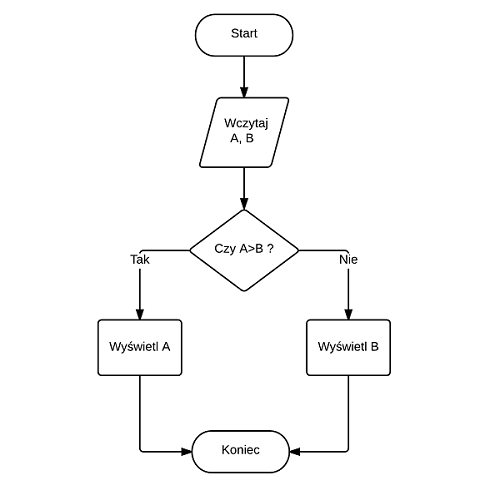
\includegraphics{algo.png}\hfill}

Co więcej warunki takie mogą być bardziej rozgałęzione, czyli np. możemy sprawdzić, czy wczytana liczba jest większa, mniejsza, czy równa 0 itd.


\subsection{Instrukcja if else}
\label{sterowanie:instrukcja-if-else}
Podstawową strukturą sterującą w większości języków programowania, w tym także w Javie jest instrukcja if. W swojej najprostszej formie odpowiada ona sytuacji, którą widzisz na wcześniejszym diagramie - pozwala sprawdzić prosty warunek, który w wyniku powinien zwrócić wartość typu boolean, czyli true lub false i na podstawie tego zadecydować, co nasz program zrobi dalej.

Ogólna konstrukcja bloku if wygląda następująco:

\emph{plik Main.java}

\begin{Verbatim}[commandchars=\\\{\},numbers=left,firstnumber=1,stepnumber=1]
\PYG{k}{if}\PYG{o}{(}\PYG{n}{warunek}\PYG{o}{)} \PYG{o}{\PYGZob{}}
  \PYG{c+c1}{//działania, gdy warunek zwraca true}
\PYG{o}{\PYGZcb{}} \PYG{k}{else} \PYG{o}{\PYGZob{}}
  \PYG{c+c1}{//działania, gdy warunek zwraca false}
\PYG{o}{\PYGZcb{}}
\end{Verbatim}

\textbf{Ćwiczenie} \emph{(5 minut)}
\begin{quote}

Zaimplementuj program, który służy do porównywania dwóch liczb całkowitych zgodny z przedstawionym wyżej diagramem. Wyświetl na ekranie komunikat o tym, która liczba jest większa od której. Liczby wczytaj do wcześniej zadeklarowanych zmiennych.
\end{quote}

\begin{Verbatim}[commandchars=\\\{\},numbers=left,firstnumber=1,stepnumber=1]
\PYG{k+kd}{public} \PYG{k+kd}{class} \PYG{n+nc}{Main} \PYG{o}{\PYGZob{}}
    \PYG{k+kd}{public} \PYG{k+kd}{static} \PYG{k+kt}{void} \PYG{n+nf}{main}\PYG{o}{(}\PYG{n}{String}\PYG{o}{[}\PYG{o}{]} \PYG{n}{args}\PYG{o}{)} \PYG{o}{\PYGZob{}}
        \PYG{k+kt}{int} \PYG{n}{a} \PYG{o}{=} \PYG{l+m+mi}{10}\PYG{o}{;}
        \PYG{k+kt}{int} \PYG{n}{b} \PYG{o}{=} \PYG{l+m+mi}{11}\PYG{o}{;}

        \PYG{k}{if} \PYG{o}{(}\PYG{n}{a} \PYG{o}{\PYGZgt{}} \PYG{n}{b}\PYG{o}{)} \PYG{o}{\PYGZob{}}
            \PYG{n}{System}\PYG{o}{.}\PYG{n+na}{out}\PYG{o}{.}\PYG{n+na}{println}\PYG{o}{(}\PYG{l+s}{\PYGZdq{}A jest większe od B \PYGZdq{}} \PYG{o}{+} \PYG{n}{a} \PYG{o}{+} \PYG{l+s}{\PYGZdq{} \PYGZgt{} \PYGZdq{}} \PYG{o}{+} \PYG{n}{b}\PYG{o}{)}\PYG{o}{;}
        \PYG{o}{\PYGZcb{}} \PYG{k}{else} \PYG{o}{\PYGZob{}}
            \PYG{n}{System}\PYG{o}{.}\PYG{n+na}{out}\PYG{o}{.}\PYG{n+na}{println}\PYG{o}{(}\PYG{l+s}{\PYGZdq{}B jest większe od A \PYGZdq{}} \PYG{o}{+} \PYG{n}{b} \PYG{o}{+} \PYG{l+s}{\PYGZdq{} \PYGZgt{} \PYGZdq{}} \PYG{o}{+} \PYG{n}{a}\PYG{o}{)}\PYG{o}{;}
        \PYG{o}{\PYGZcb{}}
    \PYG{o}{\PYGZcb{}}
\PYG{o}{\PYGZcb{}}
\end{Verbatim}

W nawiasie występującym po instrukcji if musi znajdować się wyrażenie, które w wyniku zwraca true lub false. Nie musi to być jedynie porównanie dwóch liczb tak jak w powyższym przykładzie, ale także bardziej złożony warunek np. wykorzystujący operatory logiczne \&\& lub \textbar{}\textbar{}.

W przypadku kodu tak prostego jak ten powyżej, gdzie w bloku if oraz else pomiędzy nawiasami klamrowymi znajduje się jedynie jedna instrukcja (np. \emph{System.out.print()}), nawiasy klamrowe można pominąć, czyli uprościć nasz kod do postaci:

\begin{Verbatim}[commandchars=\\\{\},numbers=left,firstnumber=1,stepnumber=1]
\PYG{k+kd}{public} \PYG{k+kd}{class} \PYG{n+nc}{Main} \PYG{o}{\PYGZob{}}
    \PYG{k+kd}{public} \PYG{k+kd}{static} \PYG{k+kt}{void} \PYG{n+nf}{main}\PYG{o}{(}\PYG{n}{String}\PYG{o}{[}\PYG{o}{]} \PYG{n}{args}\PYG{o}{)} \PYG{o}{\PYGZob{}}
        \PYG{k+kt}{int} \PYG{n}{a} \PYG{o}{=} \PYG{l+m+mi}{10}\PYG{o}{;}
        \PYG{k+kt}{int} \PYG{n}{b} \PYG{o}{=} \PYG{l+m+mi}{11}\PYG{o}{;}

        \PYG{k}{if} \PYG{o}{(}\PYG{n}{a} \PYG{o}{\PYGZgt{}} \PYG{n}{b}\PYG{o}{)}
            \PYG{n}{System}\PYG{o}{.}\PYG{n+na}{out}\PYG{o}{.}\PYG{n+na}{println}\PYG{o}{(}\PYG{l+s}{\PYGZdq{}A jest większe od B \PYGZdq{}} \PYG{o}{+} \PYG{n}{a} \PYG{o}{+} \PYG{l+s}{\PYGZdq{} \PYGZgt{} \PYGZdq{}} \PYG{o}{+} \PYG{n}{b}\PYG{o}{)}\PYG{o}{;}
        \PYG{k}{else}
            \PYG{n}{System}\PYG{o}{.}\PYG{n+na}{out}\PYG{o}{.}\PYG{n+na}{println}\PYG{o}{(}\PYG{l+s}{\PYGZdq{}B jest większe od A \PYGZdq{}} \PYG{o}{+} \PYG{n}{b} \PYG{o}{+} \PYG{l+s}{\PYGZdq{} \PYGZgt{} \PYGZdq{}} \PYG{o}{+} \PYG{n}{a}\PYG{o}{)}\PYG{o}{;}
    \PYG{o}{\PYGZcb{}}
\PYG{o}{\PYGZcb{}}
\end{Verbatim}

W praktyce jednak stosowanie klamer podnosi czytelność kodu, więc warto je stosować nawet w najbardziej trywialnych sytuacjach.

Możliwe, że zauważyłeś, że powyższy kod ma jedną poważną wadę. W przypadku, gdy liczby a i b będą identyczne, to ich porównanie za pomocą znaku ostrej nierówności zwróci false. W takiej sytuacji wyświetlony zostanie komunikat o tym, że liczba B jest większa od A, a to oczywiście nie jest prawdą.

W takim przypadku możemy zastosować np. zagnieżdżone instrukcje if.

\textbf{Ćwiczenie} \emph{(5 minut)}
\begin{quote}

Popraw wcześniejszy kod w taki sposób, aby najpierw sprawdzić, czy liczby są równe, a dopiero gdy nie są, porównaj je operatorem nierówności. Wykorzystaj zagnieżdżone warunki if i w każdej sytuacji wyświetl na ekranie stosowny komunikat.
\end{quote}

\begin{Verbatim}[commandchars=\\\{\},numbers=left,firstnumber=1,stepnumber=1]
\PYG{k+kd}{public} \PYG{k+kd}{class} \PYG{n+nc}{Main} \PYG{o}{\PYGZob{}}
    \PYG{k+kd}{public} \PYG{k+kd}{static} \PYG{k+kt}{void} \PYG{n+nf}{main}\PYG{o}{(}\PYG{n}{String}\PYG{o}{[}\PYG{o}{]} \PYG{n}{args}\PYG{o}{)} \PYG{o}{\PYGZob{}}
        \PYG{k+kt}{int} \PYG{n}{a} \PYG{o}{=} \PYG{l+m+mi}{10}\PYG{o}{;}
        \PYG{k+kt}{int} \PYG{n}{b} \PYG{o}{=} \PYG{l+m+mi}{11}\PYG{o}{;}

        \PYG{k}{if} \PYG{o}{(}\PYG{n}{a} \PYG{o}{=}\PYG{o}{=} \PYG{n}{b}\PYG{o}{)} \PYG{o}{\PYGZob{}}
            \PYG{n}{System}\PYG{o}{.}\PYG{n+na}{out}\PYG{o}{.}\PYG{n+na}{println}\PYG{o}{(}\PYG{l+s}{\PYGZdq{}Liczby A i B są równe \PYGZdq{}} \PYG{o}{+} \PYG{n}{a} \PYG{o}{+} \PYG{l+s}{\PYGZdq{} = \PYGZdq{}} \PYG{o}{+} \PYG{n}{b}\PYG{o}{)}\PYG{o}{;}
        \PYG{o}{\PYGZcb{}} \PYG{k}{else} \PYG{o}{\PYGZob{}}
            \PYG{k}{if} \PYG{o}{(}\PYG{n}{a} \PYG{o}{\PYGZgt{}} \PYG{n}{b}\PYG{o}{)} \PYG{o}{\PYGZob{}}
                \PYG{n}{System}\PYG{o}{.}\PYG{n+na}{out}\PYG{o}{.}\PYG{n+na}{println}\PYG{o}{(}\PYG{l+s}{\PYGZdq{}A jest większe od B \PYGZdq{}} \PYG{o}{+} \PYG{n}{a} \PYG{o}{+} \PYG{l+s}{\PYGZdq{} \PYGZgt{} \PYGZdq{}} \PYG{o}{+} \PYG{n}{b}\PYG{o}{)}\PYG{o}{;}
            \PYG{o}{\PYGZcb{}} \PYG{k}{else} \PYG{o}{\PYGZob{}}
                \PYG{n}{System}\PYG{o}{.}\PYG{n+na}{out}\PYG{o}{.}\PYG{n+na}{println}\PYG{o}{(}\PYG{l+s}{\PYGZdq{}B jest większe od A \PYGZdq{}} \PYG{o}{+} \PYG{n}{b} \PYG{o}{+} \PYG{l+s}{\PYGZdq{} \PYGZgt{} \PYGZdq{}} \PYG{o}{+} \PYG{n}{a}\PYG{o}{)}\PYG{o}{;}
            \PYG{o}{\PYGZcb{}}
        \PYG{o}{\PYGZcb{}}
    \PYG{o}{\PYGZcb{}}
\PYG{o}{\PYGZcb{}}
\end{Verbatim}

Powyższy kod posiada jedną, aczkolwiek istotną wadę. Nawet pojedynczo zagnieżdżone bloki instrukcji if wpływają w znaczącym stopniu na zmniejszenie czytelności kodu i w ogólności dobrą praktyką jest unikanie takich sytuacji. Najprościej jest to zrobić korzystając z nieco bardziej złożonej instrukcji if else:

\begin{Verbatim}[commandchars=\\\{\},numbers=left,firstnumber=1,stepnumber=1]
\PYG{k}{if} \PYG{o}{(}\PYG{n}{warunek1}\PYG{o}{)} \PYG{o}{\PYGZob{}}
    \PYG{c+c1}{//instrukcje gdy warunek1 jest true}
\PYG{o}{\PYGZcb{}} \PYG{k}{else} \PYG{k}{if} \PYG{o}{(}\PYG{n}{warunek2}\PYG{o}{)} \PYG{o}{\PYGZob{}}
    \PYG{c+c1}{//instrukcje gdy warunek2 jest true}
\PYG{o}{\PYGZcb{}} \PYG{k}{else} \PYG{k}{if} \PYG{o}{(}\PYG{n}{warunek3}\PYG{o}{)} \PYG{o}{\PYGZob{}}
    \PYG{c+c1}{//instrukcje gdy warunek3 jest true}
\PYG{o}{\PYGZcb{}} \PYG{k}{else} \PYG{o}{\PYGZob{}}
    \PYG{c+c1}{//instrukcje gdy żadny z warunków nie był true}
\PYG{o}{\PYGZcb{}}
\end{Verbatim}

Korzystając z dodatkowych warunków w postaci \emph{else if} możemy w dowolny sposób rozgałęzić działanie naszej aplikacji bez konieczności zagnieżdżania warunków if i obniżania czytelności kodu. Pamiętaj, że blok z warunkiem2 wykona się tylko wtedy, gdy warunek1 zwróci false, analogicznie warunek3, gdzy warunek2 oraz warunek1 będą nieprawdziwe.

\textbf{Ćwiczenie} \emph{(5 minut)}
\begin{quote}

Przerób wcześniejszy kod z porównywaniem liczb w taki sposób, aby wyeliminować zagnieżdżone warunki if.
\end{quote}

\begin{Verbatim}[commandchars=\\\{\},numbers=left,firstnumber=1,stepnumber=1]
\PYG{k+kd}{public} \PYG{k+kd}{class} \PYG{n+nc}{Main} \PYG{o}{\PYGZob{}}
    \PYG{k+kd}{public} \PYG{k+kd}{static} \PYG{k+kt}{void} \PYG{n+nf}{main}\PYG{o}{(}\PYG{n}{String}\PYG{o}{[}\PYG{o}{]} \PYG{n}{args}\PYG{o}{)} \PYG{o}{\PYGZob{}}
        \PYG{k+kt}{int} \PYG{n}{a} \PYG{o}{=} \PYG{l+m+mi}{12}\PYG{o}{;}
        \PYG{k+kt}{int} \PYG{n}{b} \PYG{o}{=} \PYG{l+m+mi}{11}\PYG{o}{;}

        \PYG{k}{if} \PYG{o}{(}\PYG{n}{a} \PYG{o}{=}\PYG{o}{=} \PYG{n}{b}\PYG{o}{)} \PYG{o}{\PYGZob{}}
            \PYG{n}{System}\PYG{o}{.}\PYG{n+na}{out}\PYG{o}{.}\PYG{n+na}{println}\PYG{o}{(}\PYG{l+s}{\PYGZdq{}Liczby A i B są równe \PYGZdq{}} \PYG{o}{+} \PYG{n}{a} \PYG{o}{+} \PYG{l+s}{\PYGZdq{} = \PYGZdq{}} \PYG{o}{+} \PYG{n}{b}\PYG{o}{)}\PYG{o}{;}
        \PYG{o}{\PYGZcb{}} \PYG{k}{else} \PYG{k}{if} \PYG{o}{(}\PYG{n}{a} \PYG{o}{\PYGZgt{}} \PYG{n}{b}\PYG{o}{)} \PYG{o}{\PYGZob{}}
            \PYG{n}{System}\PYG{o}{.}\PYG{n+na}{out}\PYG{o}{.}\PYG{n+na}{println}\PYG{o}{(}\PYG{l+s}{\PYGZdq{}A jest większe od B \PYGZdq{}} \PYG{o}{+} \PYG{n}{a} \PYG{o}{+} \PYG{l+s}{\PYGZdq{} \PYGZgt{} \PYGZdq{}} \PYG{o}{+} \PYG{n}{b}\PYG{o}{)}\PYG{o}{;}
        \PYG{o}{\PYGZcb{}} \PYG{k}{else} \PYG{o}{\PYGZob{}}
            \PYG{n}{System}\PYG{o}{.}\PYG{n+na}{out}\PYG{o}{.}\PYG{n+na}{println}\PYG{o}{(}\PYG{l+s}{\PYGZdq{}B jest większe od A \PYGZdq{}} \PYG{o}{+} \PYG{n}{b} \PYG{o}{+} \PYG{l+s}{\PYGZdq{} \PYGZgt{} \PYGZdq{}} \PYG{o}{+} \PYG{n}{a}\PYG{o}{)}\PYG{o}{;}
        \PYG{o}{\PYGZcb{}}
    \PYG{o}{\PYGZcb{}}
\PYG{o}{\PYGZcb{}}
\end{Verbatim}

Zauważ, że ponieważ wiemy, że istnieją tylko trzy możliwe wyniki porównania dwóch liczb, to w ostatnim bloku nie musimy zapisywać \emph{else if(a\textless{}b)} a wystarczy jedynie samo \emph{else} - jest to jedyny możliwy wynik jaki pozostał.


\subsection{Struktura sterująca switch}
\label{sterowanie:struktura-sterujaca-switch}
Powyżej pokazana struktura if-else-if pomimo iż bardziej czytelna od zagnieżdżonych warunków, to jednak w sytuacji, gdy mamy np. menu aplikacji składające się z 10 możliwych opcji, nie wydaje się najlepszym rozwiązaniem. W większości języków programowania rozwiązaniem tego problemu jest bardziej złożona struktura \textbf{switch}.

W odróżnieniu od instrukcji if, w strukturze switch operujemy nie na warunkach zwracających wartość true lub false, ale na liczbach całkowitych. Od Javy w wersji 7 możliwe jest także stosowanie w miejsce liczb napisów typu String.

Schematyczna budowa switch wygląda jak poniżej:

\begin{Verbatim}[commandchars=\\\{\}]
//wybrana opcja musi być typu całkowitoliczbowego lub być wartością typu String
switch (wybrana\PYGZus{}opcja) \PYGZob{}
    case wartość1:
        //instrukcje, gdy wartość1 jest równa wartości wybrana\PYGZus{}opcja
        break;
    case wartość2:
         //instrukcje, gdy wartość2 jest równa wartości wybrana\PYGZus{}opcja
        break;
    case ...
    default:
        //instrukcje, gdy żaden z wcześniejszych warunków nie pasuje do wybrana\PYGZus{}opcja
        //odpowiednik ostatniego bloku else z instrukcji if\PYGZhy{}else\PYGZhy{}if
\PYGZcb{}
\end{Verbatim}

Istotne w powyższym kodzie jest zastosowanie instrukcji break. Jeżeli jej nie zastosujesz w danym bloku case, wtedy wykonane zostaną także instrukcje z innych bloków case znajdujących się poniżej (aż do napotkania break). W bloku default nie jest to wymagane, ponieważ jest on ostatnim w całej konstrukcji i nie musimy niczego przerywać.
Dzięki instrukcji switch możemy zbudować w wygodny sposób proste menu w swojej aplikacji w stylu:

{\hfill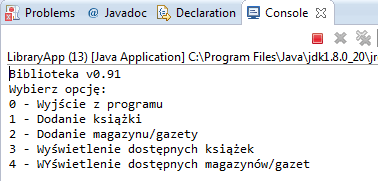
\includegraphics{library.png}\hfill}

\textbf{Ćwiczenie} \emph{(10 minut)}
\begin{quote}

Napisz prostą aplikację, w której utworzysz jedną zmienną całkowitoliczbową i przypiszesz do niej wartość z zakresu od 1 do 10. Następnie stwórz blok switch, w którym na podstawie wybranej opcji wyświetlisz wcześniej zainicjowaną zmienną podniesioną do 1, 2, 3 lub 4 potęgi.
\end{quote}

\begin{Verbatim}[commandchars=\\\{\},numbers=left,firstnumber=1,stepnumber=1]
\PYG{k+kd}{public} \PYG{k+kd}{class} \PYG{n+nc}{Exponential} \PYG{o}{\PYGZob{}}
    \PYG{k+kd}{public} \PYG{k+kd}{static} \PYG{k+kt}{void} \PYG{n+nf}{main}\PYG{o}{(}\PYG{n}{String}\PYG{o}{[}\PYG{o}{]} \PYG{n}{args}\PYG{o}{)} \PYG{o}{\PYGZob{}}
        \PYG{k+kt}{int} \PYG{n}{number} \PYG{o}{=} \PYG{l+m+mi}{5}\PYG{o}{;}

        \PYG{k+kt}{int} \PYG{n}{option} \PYG{o}{=} \PYG{l+m+mi}{2}\PYG{o}{;}

        \PYG{k}{switch} \PYG{o}{(}\PYG{n}{option}\PYG{o}{)} \PYG{o}{\PYGZob{}}
        \PYG{k}{case} \PYG{l+m+mi}{1}\PYG{o}{:}
            \PYG{n}{System}\PYG{o}{.}\PYG{n+na}{out}\PYG{o}{.}\PYG{n+na}{println}\PYG{o}{(}\PYG{n}{number} \PYG{o}{+} \PYG{l+s}{\PYGZdq{} do potęgi 1 = \PYGZdq{}} \PYG{o}{+} \PYG{n}{number}\PYG{o}{)}\PYG{o}{;}
            \PYG{k}{break}\PYG{o}{;}
        \PYG{k}{case} \PYG{l+m+mi}{2}\PYG{o}{:}
            \PYG{n}{System}\PYG{o}{.}\PYG{n+na}{out}\PYG{o}{.}\PYG{n+na}{println}\PYG{o}{(}\PYG{n}{number} \PYG{o}{+} \PYG{l+s}{\PYGZdq{} do potęgi 2 = \PYGZdq{}} \PYG{o}{+} \PYG{n}{number}\PYG{o}{*}\PYG{n}{number}\PYG{o}{)}\PYG{o}{;}
            \PYG{k}{break}\PYG{o}{;}
        \PYG{k}{case} \PYG{l+m+mi}{3}\PYG{o}{:}
            \PYG{n}{System}\PYG{o}{.}\PYG{n+na}{out}\PYG{o}{.}\PYG{n+na}{println}\PYG{o}{(}\PYG{n}{number} \PYG{o}{+} \PYG{l+s}{\PYGZdq{} do potęgi 3 = \PYGZdq{}} \PYG{o}{+} \PYG{n}{number}\PYG{o}{*}\PYG{n}{number}\PYG{o}{*}\PYG{n}{number}\PYG{o}{)}\PYG{o}{;}
            \PYG{k}{break}\PYG{o}{;}
        \PYG{k}{case} \PYG{l+m+mi}{4}\PYG{o}{:}
            \PYG{n}{System}\PYG{o}{.}\PYG{n+na}{out}\PYG{o}{.}\PYG{n+na}{println}\PYG{o}{(}\PYG{n}{number} \PYG{o}{+} \PYG{l+s}{\PYGZdq{} do potęgi 4 = \PYGZdq{}} \PYG{o}{+} \PYG{n}{number}\PYG{o}{*}\PYG{n}{number}\PYG{o}{*}\PYG{n}{number}\PYG{o}{*}\PYG{n}{number}\PYG{o}{)}\PYG{o}{;}
            \PYG{k}{break}\PYG{o}{;}
        \PYG{k}{default}\PYG{o}{:}
            \PYG{n}{System}\PYG{o}{.}\PYG{n+na}{out}\PYG{o}{.}\PYG{n+na}{println}\PYG{o}{(}\PYG{l+s}{\PYGZdq{}Wybrano niepoprawną opcję\PYGZdq{}}\PYG{o}{)}\PYG{o}{;}
        \PYG{o}{\PYGZcb{}}
    \PYG{o}{\PYGZcb{}}
\PYG{o}{\PYGZcb{}}
\end{Verbatim}


\subsection{Pętle while i do while}
\label{sterowanie:petle-while-i-do-while}
W pierwszej części kursu dowiedziałeś się, że w Javie istnieją specjalne struktury danych, które pozwalają przechowywać wiele wartości tego samego typu, które nazwaliśmy tablicami. W tym miejscu powrócimy do nich na chwilę, aby pokazać, że ich przetwarzanie, czy wyświetlanie może być znacznie krótsze i do każdego elementu tablicy nie musimy odwoływać się osobno tak jak do zwykłych zmiennych.

Dwa pierwsze rodzaje pętli, które omówimy to \textbf{while} oraz \textbf{do while}. Różnica między nimi jest subtelna, aczkolwiek wpływa w znaczący sposób na to co dzieje się w naszym programie. Ogólna postać obu pętli wygląda jak poniżej:

\begin{Verbatim}[commandchars=\\\{\},numbers=left,firstnumber=1,stepnumber=1]
\PYG{c+c1}{//pętla while}
\PYG{k}{while} \PYG{o}{(}\PYG{n}{warunek}\PYG{o}{)} \PYG{o}{\PYGZob{}}
    \PYG{c+c1}{//instrukcje, które będą powtarzane tak długo, dopóki warunek zwraca true}
\PYG{o}{\PYGZcb{}}

\PYG{c+c1}{//pętla do while}
\PYG{k}{do}\PYG{o}{\PYGZob{}}
    \PYG{c+c1}{//instrukcje, które będą się wykonywały tak długo, dopóki warunek zwraca true}
\PYG{o}{\PYGZcb{}} \PYG{k}{while}\PYG{o}{(}\PYG{n}{warunek}\PYG{o}{)}\PYG{o}{;}
\end{Verbatim}

Różnica pomiędzy dwoma wyżej pokazanymi rodzajami pętli polega na tym, że w przypadku zwykłej pętli while warunek jest sprawdzany przed rozpoczęciem ciała pętli, więc jeżeli warunek nie będzie prawdziwy, to zawartość pętli nie wykona się ani razu. W przypadku pętli do while mamy pewność, że instrukcje w jej ciele wykonają się co najmniej raz, ponieważ warunek sprawdzany jest dopiero na końcu.
W miejscu wyrażenia, które w powyższym kodzie nazwaliśmy jako \emph{warunek} należy wstawić dowolną zmienną typu boolean lub wyrażenie logiczne zwracające true lub false.

\textbf{Ćwiczenie} \emph{(10 minut)}
\begin{quote}

Napisz program, w którym zadeklarujesz tablicę 50 liczb całkowitych. Wypełnij ją przy pomocy pętli while wartościami od 1 do 50, a następnie wyświetl jej kolejne elementy za pomocą pętli do while.
\end{quote}

\emph{plik Loops1.java}

\begin{Verbatim}[commandchars=\\\{\},numbers=left,firstnumber=1,stepnumber=1]
\PYG{k+kd}{public} \PYG{k+kd}{class} \PYG{n+nc}{Loops1} \PYG{o}{\PYGZob{}}
    \PYG{k+kd}{public} \PYG{k+kd}{static} \PYG{k+kt}{void} \PYG{n+nf}{main}\PYG{o}{(}\PYG{n}{String}\PYG{o}{[}\PYG{o}{]} \PYG{n}{args}\PYG{o}{)} \PYG{o}{\PYGZob{}}
        \PYG{k+kt}{int}\PYG{o}{[}\PYG{o}{]} \PYG{n}{array} \PYG{o}{=} \PYG{k}{new} \PYG{k+kt}{int}\PYG{o}{[}\PYG{l+m+mi}{50}\PYG{o}{]}\PYG{o}{;}

        \PYG{k+kt}{int} \PYG{n}{i} \PYG{o}{=} \PYG{l+m+mi}{0}\PYG{o}{;} \PYG{c+c1}{// licznik pętli}

        \PYG{c+c1}{// wypełniamy tablicę}
        \PYG{k}{while} \PYG{o}{(}\PYG{n}{i} \PYG{o}{\PYGZlt{}} \PYG{n}{array}\PYG{o}{.}\PYG{n+na}{length}\PYG{o}{)} \PYG{o}{\PYGZob{}}
            \PYG{n}{array}\PYG{o}{[}\PYG{n}{i}\PYG{o}{]} \PYG{o}{=} \PYG{n}{i} \PYG{o}{+} \PYG{l+m+mi}{1}\PYG{o}{;}
            \PYG{n}{i} \PYG{o}{=} \PYG{n}{i} \PYG{o}{+} \PYG{l+m+mi}{1}\PYG{o}{;}
        \PYG{o}{\PYGZcb{}}

        \PYG{c+c1}{// zerujemy licznik}
        \PYG{n}{i} \PYG{o}{=} \PYG{l+m+mi}{0}\PYG{o}{;}

        \PYG{c+c1}{//wyświetlamy wartości}
        \PYG{k}{do} \PYG{o}{\PYGZob{}}
            \PYG{n}{System}\PYG{o}{.}\PYG{n+na}{out}\PYG{o}{.}\PYG{n+na}{print}\PYG{o}{(}\PYG{n}{array}\PYG{o}{[}\PYG{n}{i}\PYG{o}{]} \PYG{o}{+} \PYG{l+s}{\PYGZdq{}; \PYGZdq{}}\PYG{o}{)}\PYG{o}{;}
            \PYG{n}{i} \PYG{o}{=} \PYG{n}{i} \PYG{o}{+} \PYG{l+m+mi}{1}\PYG{o}{;}
        \PYG{o}{\PYGZcb{}} \PYG{k}{while} \PYG{o}{(}\PYG{n}{i} \PYG{o}{\PYGZlt{}} \PYG{n}{array}\PYG{o}{.}\PYG{n+na}{length}\PYG{o}{)}\PYG{o}{;}
    \PYG{o}{\PYGZcb{}}
\PYG{o}{\PYGZcb{}}
\end{Verbatim}

Do rozwiązania należało zastosować scenariusz, który będzie się często powtarzał w niemal każdej aplikacji, która korzysta z tablic:
\begin{enumerate}
\item {} 
Utworzenie tablicy

\item {} 
Zainicjowanie licznika pętli

\item {} 
Wypełnienie kolejnych komórek tablicy wartościami (while)

\item {} 
Wykonanie operacji na danych w tablicy (pętla do while)

\end{enumerate}

W praktyce dużo częściej stosuje się pętle while, ponieważ są po prostu bardziej intuicyjne


\subsection{Inkrementacja i dekrementacja}
\label{sterowanie:inkrementacja-i-dekrementacja}
Operacją, która w przypadku pętli będzie się bardzo często powtarzała jest zwiększanie lub zmniejszanie zmiennej reprezentującej licznik o 1. W programowaniu jest to tak często wykorzystywane, że powstały specjalne operatory, które skracają zapis, a po pewnym czasie stają się nawykiem przy pisaniu pętli.

\textbf{Inkrementacja} to zwiększenie wartości zmiennej o 1, natomiast \textbf{dekrementacja} to zmniejszenie o 1. Inkrementację oznaczamy znakiem podwójnego plusa (++), natomiast dekrementację podwójnego minusa (--).

W praktyce wygląda to następująco:

\begin{Verbatim}[commandchars=\\\{\},numbers=left,firstnumber=1,stepnumber=1]
\PYG{k+kt}{int} \PYG{n}{a} \PYG{o}{=} \PYG{l+m+mi}{1}\PYG{o}{;}
\PYG{n}{a}\PYG{o}{+}\PYG{o}{+}\PYG{o}{;}
\PYG{c+c1}{//a ma teraz wartość 2}
\PYG{n}{a}\PYG{o}{\PYGZhy{}}\PYG{o}{\PYGZhy{}}\PYG{o}{;}
\PYG{c+c1}{//a ma teraz znowu wartość 1}
\end{Verbatim}

Dodatkowo istnieją dwa rodzaje powyższych operatorów. W formie przyrostkowej, czyli np. a++ oraz przedrostkowej, czyli ++a. Różnica polega na tym, kiedy wykonywane jest faktyczne zwiększenie, czy zmniejszenie wartości o 1. W przypadku inkrementacji przyrostkowej wartość zmiennej jest zwiększana dopiero po wykonaniu operacji, w której zmienna ta występuje.

Najłatwiej zobrazować to prostym przykładem:

\begin{Verbatim}[commandchars=\\\{\},numbers=left,firstnumber=1,stepnumber=1]
\PYG{k+kt}{int} \PYG{n}{x} \PYG{o}{=} \PYG{l+m+mi}{1}\PYG{o}{;}
\PYG{n}{System}\PYG{o}{.}\PYG{n+na}{out}\PYG{o}{.}\PYG{n+na}{println}\PYG{o}{(}\PYG{n}{x}\PYG{o}{)}\PYG{o}{;} \PYG{c+c1}{//wyświetla 1}
\PYG{n}{System}\PYG{o}{.}\PYG{n+na}{out}\PYG{o}{.}\PYG{n+na}{println}\PYG{o}{(}\PYG{n}{x}\PYG{o}{+}\PYG{o}{+}\PYG{o}{)}\PYG{o}{;} \PYG{c+c1}{//również wyświetla 1, ale po wyświetleniu zwiększa wartość x do 2}
\PYG{n}{System}\PYG{o}{.}\PYG{n+na}{out}\PYG{o}{.}\PYG{n+na}{println}\PYG{o}{(}\PYG{n}{x}\PYG{o}{)}\PYG{o}{;} \PYG{c+c1}{//wyświetla 2}
\end{Verbatim}

Analogicznie dla inkrementacji przedrostkowej:

\begin{Verbatim}[commandchars=\\\{\},numbers=left,firstnumber=1,stepnumber=1]
\PYG{k+kt}{int} \PYG{n}{x} \PYG{o}{=} \PYG{l+m+mi}{1}\PYG{o}{;}
\PYG{n}{System}\PYG{o}{.}\PYG{n+na}{out}\PYG{o}{.}\PYG{n+na}{println}\PYG{o}{(}\PYG{n}{x}\PYG{o}{)}\PYG{o}{;} \PYG{c+c1}{//wyświetla 1}
\PYG{n}{System}\PYG{o}{.}\PYG{n+na}{out}\PYG{o}{.}\PYG{n+na}{println}\PYG{o}{(}\PYG{o}{+}\PYG{o}{+}\PYG{n}{x}\PYG{o}{)}\PYG{o}{;} \PYG{c+c1}{//najpierw zwiększa wartość x do 2 i wyświetla 2}
\PYG{n}{System}\PYG{o}{.}\PYG{n+na}{out}\PYG{o}{.}\PYG{n+na}{println}\PYG{o}{(}\PYG{n}{x}\PYG{o}{)}\PYG{o}{;} \PYG{c+c1}{//wyświetla 2}
\end{Verbatim}

W pętlach znajduje to takie zastosowanie, że możemy pominąć ręczne zwiększanie licznika w postaci \emph{i = i+1} i zapisać \emph{i++}, dodatkowo w niektórych sytuacjach bezpośrednio przy sprawdzaniu warunku, np.:

\begin{Verbatim}[commandchars=\\\{\}]
\PYG{k+kt}{int} \PYG{n}{i}\PYG{o}{=}\PYG{l+m+mi}{0}\PYG{o}{;}
\PYG{k}{while}\PYG{o}{(}\PYG{n}{i}\PYG{o}{+}\PYG{o}{+} \PYG{o}{\PYGZlt{}} \PYG{l+m+mi}{10}\PYG{o}{)} \PYG{o}{\PYGZob{}} \PYG{o}{.}\PYG{o}{.}\PYG{o}{.} \PYG{o}{\PYGZcb{}}
\end{Verbatim}

\textbf{Ćwiczenie} \emph{(5 minut)}
\begin{quote}

Przerób poprzedni przykład z wypełnianiem tablicy w taki sposób, aby wykorzystać operator inkrementacji. Dodatkowo wartości w tablicy wyświetl od końca wykorzystując dekrementację.
\end{quote}

\begin{Verbatim}[commandchars=\\\{\},numbers=left,firstnumber=1,stepnumber=1]
\PYG{k+kd}{public} \PYG{k+kd}{class} \PYG{n+nc}{Loops1Increment} \PYG{o}{\PYGZob{}}
    \PYG{k+kd}{public} \PYG{k+kd}{static} \PYG{k+kt}{void} \PYG{n+nf}{main}\PYG{o}{(}\PYG{n}{String}\PYG{o}{[}\PYG{o}{]} \PYG{n}{args}\PYG{o}{)} \PYG{o}{\PYGZob{}}
        \PYG{k+kt}{int}\PYG{o}{[}\PYG{o}{]} \PYG{n}{array} \PYG{o}{=} \PYG{k}{new} \PYG{k+kt}{int}\PYG{o}{[}\PYG{l+m+mi}{50}\PYG{o}{]}\PYG{o}{;}

        \PYG{k+kt}{int} \PYG{n}{i} \PYG{o}{=} \PYG{l+m+mi}{0}\PYG{o}{;} \PYG{c+c1}{// licznik pętli}

        \PYG{c+c1}{// wypełniamy tablicę}
        \PYG{k}{while} \PYG{o}{(}\PYG{n}{i} \PYG{o}{\PYGZlt{}} \PYG{n}{array}\PYG{o}{.}\PYG{n+na}{length}\PYG{o}{)} \PYG{o}{\PYGZob{}}
            \PYG{n}{array}\PYG{o}{[}\PYG{n}{i}\PYG{o}{]} \PYG{o}{=} \PYG{n}{i} \PYG{o}{+} \PYG{l+m+mi}{1}\PYG{o}{;}
            \PYG{n}{i}\PYG{o}{+}\PYG{o}{+}\PYG{o}{;}
        \PYG{o}{\PYGZcb{}}

        \PYG{c+c1}{// przypisujemy do licznika ostatni indeks tablicy}
        \PYG{n}{i} \PYG{o}{=} \PYG{n}{array}\PYG{o}{.}\PYG{n+na}{length}\PYG{o}{\PYGZhy{}}\PYG{l+m+mi}{1}\PYG{o}{;}

        \PYG{c+c1}{//wyświetlamy wartości}
        \PYG{k}{do} \PYG{o}{\PYGZob{}}
            \PYG{n}{System}\PYG{o}{.}\PYG{n+na}{out}\PYG{o}{.}\PYG{n+na}{print}\PYG{o}{(}\PYG{n}{array}\PYG{o}{[}\PYG{n}{i}\PYG{o}{]} \PYG{o}{+} \PYG{l+s}{\PYGZdq{}; \PYGZdq{}}\PYG{o}{)}\PYG{o}{;}
        \PYG{o}{\PYGZcb{}} \PYG{k}{while} \PYG{o}{(}\PYG{n}{i}\PYG{o}{\PYGZhy{}}\PYG{o}{\PYGZhy{}} \PYG{o}{\PYGZgt{}} \PYG{l+m+mi}{0}\PYG{o}{)}\PYG{o}{;}
    \PYG{o}{\PYGZcb{}}
\PYG{o}{\PYGZcb{}}
\end{Verbatim}

Pętla while nie zmieniła się znacząco, jedynie zamieniliśmy sposób zwiększania zmiennej i. W pętli do while zastosowaliśmy dekrementacją, a dodatkowo zmieniliśmy warunek, na taki, który pozwala nam wyświetlać wartości od ostatniego indeksu tablicy, do pierwszego (czyli 0 zgodnie z indeksowaniem tablic).


\subsection{Pętle for i for each}
\label{sterowanie:petle-for-i-for-each}
Pętle for i for each to dwa kolejne rodzaje pętli, które idealnie znajdują zastosowanie w przypadku kolekcji danych o znanych z góry rozmiarach, czyli np. pętlach. Ich specyficzna konstrukcja sprawia, że powinniśmy je stosować przede wszystkim w sytuacjach, gdy chcemy przeglądnąć całą kolekcję elementów.

Schematyczna budowa pętli for:

\begin{Verbatim}[commandchars=\\\{\},numbers=left,firstnumber=1,stepnumber=1]
\PYG{k}{for}\PYG{o}{(}\PYG{n}{inicjalizacja\PYGZus{}licznika}\PYG{o}{;} \PYG{n}{warunek\PYGZus{}stopu}\PYG{o}{;} \PYG{n}{zmiana\PYGZus{}licznika}\PYG{o}{)} \PYG{o}{\PYGZob{}}
    \PYG{c+c1}{//operacje}
\PYG{o}{\PYGZcb{}}
\end{Verbatim}

Zwróć uwagę, że w nawiasach okrągłych znajdują się trzy elementy, które są oddzielone od siebie średnikami. W sytuacji, gdy chcielibyśmy uzupełnić tablicę o rozmiarze 10 liczbami 10, 20, 30, ..., 100, można to zrobić w następujący sposób:

\begin{Verbatim}[commandchars=\\\{\},numbers=left,firstnumber=1,stepnumber=1]
\PYG{k+kd}{public} \PYG{k+kd}{class} \PYG{n+nc}{ForLoop} \PYG{o}{\PYGZob{}}
    \PYG{k+kd}{public} \PYG{k+kd}{static} \PYG{k+kt}{void} \PYG{n+nf}{main}\PYG{o}{(}\PYG{n}{String}\PYG{o}{[}\PYG{o}{]} \PYG{n}{args}\PYG{o}{)} \PYG{o}{\PYGZob{}}
        \PYG{k+kt}{int}\PYG{o}{[}\PYG{o}{]} \PYG{n}{array} \PYG{o}{=} \PYG{k}{new} \PYG{k+kt}{int}\PYG{o}{[}\PYG{l+m+mi}{10}\PYG{o}{]}\PYG{o}{;}

        \PYG{k}{for}\PYG{o}{(}\PYG{k+kt}{int} \PYG{n}{i}\PYG{o}{=}\PYG{l+m+mi}{0}\PYG{o}{;} \PYG{n}{i} \PYG{o}{\PYGZlt{}} \PYG{n}{array}\PYG{o}{.}\PYG{n+na}{length}\PYG{o}{;} \PYG{n}{i}\PYG{o}{+}\PYG{o}{+}\PYG{o}{)} \PYG{o}{\PYGZob{}}
            \PYG{n}{array}\PYG{o}{[}\PYG{n}{i}\PYG{o}{]} \PYG{o}{=} \PYG{o}{(}\PYG{n}{i}\PYG{o}{+}\PYG{l+m+mi}{1}\PYG{o}{)}\PYG{o}{*}\PYG{l+m+mi}{10}\PYG{o}{;}
        \PYG{o}{\PYGZcb{}}
    \PYG{o}{\PYGZcb{}}
\PYG{o}{\PYGZcb{}}
\end{Verbatim}

W porównaniu do pętli while i do while zapis taki staje się bardziej czytelny, ponieważ wszystkie elementy bezpośrednio związane z pętlą, czyli zmienna licznika i warunek końca pętli są zawarte bezpośrednio w deklaracji pętli obok siebie. Będzie to przydatne, gdy kod w pętli będzie nieco bardziej rozbudowany.

Istnieje także odmiana pętli for, która przeznaczona jest wyłącznie do operacji na kolekcjach, gdzie znacząco uproszczono kwestie związane z licznikiem, czy jakimikolwiek warunkami stopu. Jedynym zadaniem pętli for each, o której mowa, jest przejście po wszystkich elementach kolekcji.

Schematyczna budowa pętli for each:

\begin{Verbatim}[commandchars=\\\{\}]
\PYG{k}{for}\PYG{o}{(}\PYG{n}{typ\PYGZus{}zmiennej} \PYG{n+nl}{zmienna:} \PYG{n}{kolekcja}\PYG{o}{)} \PYG{o}{\PYGZob{}}
    \PYG{n}{operacje} \PYG{n}{na} \PYG{n}{zmiennej}
\PYG{o}{\PYGZcb{}}
\end{Verbatim}

Typ zmiennej musi być zgodny z typem kolekcji (czyli np. tablicy), ponieważ w kolejnych iteracjach przypisywana będzie do niej kolejna jej wartość.

Przykładowo dodajmy do poprzedniego przykładu opcję wydruku danych na ekranie z użyciem pętli for each:

\begin{Verbatim}[commandchars=\\\{\},numbers=left,firstnumber=1,stepnumber=1]
\PYG{k+kd}{public} \PYG{k+kd}{class} \PYG{n+nc}{ForLoop} \PYG{o}{\PYGZob{}}
    \PYG{k+kd}{public} \PYG{k+kd}{static} \PYG{k+kt}{void} \PYG{n+nf}{main}\PYG{o}{(}\PYG{n}{String}\PYG{o}{[}\PYG{o}{]} \PYG{n}{args}\PYG{o}{)} \PYG{o}{\PYGZob{}}
        \PYG{k+kt}{int}\PYG{o}{[}\PYG{o}{]} \PYG{n}{array} \PYG{o}{=} \PYG{k}{new} \PYG{k+kt}{int}\PYG{o}{[}\PYG{l+m+mi}{10}\PYG{o}{]}\PYG{o}{;}

        \PYG{k}{for}\PYG{o}{(}\PYG{k+kt}{int} \PYG{n}{i}\PYG{o}{=}\PYG{l+m+mi}{0}\PYG{o}{;} \PYG{n}{i} \PYG{o}{\PYGZlt{}} \PYG{n}{array}\PYG{o}{.}\PYG{n+na}{length}\PYG{o}{;} \PYG{n}{i}\PYG{o}{+}\PYG{o}{+}\PYG{o}{)} \PYG{o}{\PYGZob{}}
            \PYG{n}{array}\PYG{o}{[}\PYG{n}{i}\PYG{o}{]} \PYG{o}{=} \PYG{o}{(}\PYG{n}{i}\PYG{o}{+}\PYG{l+m+mi}{1}\PYG{o}{)}\PYG{o}{*}\PYG{l+m+mi}{10}\PYG{o}{;}
        \PYG{o}{\PYGZcb{}}

        \PYG{k}{for}\PYG{o}{(}\PYG{k+kt}{int} \PYG{n+nl}{number:} \PYG{n}{array}\PYG{o}{)} \PYG{o}{\PYGZob{}}
            \PYG{n}{System}\PYG{o}{.}\PYG{n+na}{out}\PYG{o}{.}\PYG{n+na}{print}\PYG{o}{(}\PYG{n}{number} \PYG{o}{+} \PYG{l+s}{\PYGZdq{}; \PYGZdq{}}\PYG{o}{)}\PYG{o}{;}
        \PYG{o}{\PYGZcb{}}
    \PYG{o}{\PYGZcb{}}
\PYG{o}{\PYGZcb{}}
\end{Verbatim}

Ponieważ nasza tablica była typu int{[}{]} to zmienna \emph{number} została zadeklarowana jako int. Możemy ją wykorzystać następnie w naszej pętli.

\begin{notice}{attention}{Attention:}
Pamiętaj, że pętlę for each najlepiej jest stosować wyłącznie do operacji odczytu kolekcji, a nie jej modyfikacji. Do zmiennej deklarowanej w pętli przypisywana jest w rzeczywistości kopia wartości (lub referencji obiektu) przechowywanej w kolekcji, więc modyfikując ją nie modyfikujesz oryginalnej wartości.
\end{notice}


\subsection{Ćwiczenie podsumowujące}
\label{sterowanie:cwiczenie-podsumowujace}
Napisz program w którym wyświetlisz na ekranie zawartość tablicy dwuwymiarowej o rozmiarach NxN (gdzie rozmiar N jest wartością przechowywaną w zmiennej, którą można modyfikować). Tablica powinna być wypełniona znakami ``0'' (zero), jedynie na krawędziach oraz przekątnych powinny znajdować się znaki ``X''. Do wypełnienia tablicy zastosuj pętle for, natomiast do wyświetlenia jej zawartości pętle while. Używaj w kodzie tam gdzie to możliwe operatorów inkrementacji.
Przykładowy wydruk programu:

\begin{Verbatim}[commandchars=\\\{\}]
\PYG{n}{X} \PYG{n}{X} \PYG{n}{X} \PYG{n}{X} \PYG{n}{X} \PYG{n}{X} \PYG{n}{X} \PYG{n}{X}
\PYG{n}{X} \PYG{n}{X} \PYG{l+m+mi}{0} \PYG{l+m+mi}{0} \PYG{l+m+mi}{0} \PYG{l+m+mi}{0} \PYG{n}{X} \PYG{n}{X}
\PYG{n}{X} \PYG{l+m+mi}{0} \PYG{n}{X} \PYG{l+m+mi}{0} \PYG{l+m+mi}{0} \PYG{n}{X} \PYG{l+m+mi}{0} \PYG{n}{X}
\PYG{n}{X} \PYG{l+m+mi}{0} \PYG{l+m+mi}{0} \PYG{n}{X} \PYG{n}{X} \PYG{l+m+mi}{0} \PYG{l+m+mi}{0} \PYG{n}{X}
\PYG{n}{X} \PYG{l+m+mi}{0} \PYG{l+m+mi}{0} \PYG{n}{X} \PYG{n}{X} \PYG{l+m+mi}{0} \PYG{l+m+mi}{0} \PYG{n}{X}
\PYG{n}{X} \PYG{l+m+mi}{0} \PYG{n}{X} \PYG{l+m+mi}{0} \PYG{l+m+mi}{0} \PYG{n}{X} \PYG{l+m+mi}{0} \PYG{n}{X}
\PYG{n}{X} \PYG{n}{X} \PYG{l+m+mi}{0} \PYG{l+m+mi}{0} \PYG{l+m+mi}{0} \PYG{l+m+mi}{0} \PYG{n}{X} \PYG{n}{X}
\PYG{n}{X} \PYG{n}{X} \PYG{n}{X} \PYG{n}{X} \PYG{n}{X} \PYG{n}{X} \PYG{n}{X} \PYG{n}{X}
\end{Verbatim}

\emph{plik Zad1.java}

\begin{Verbatim}[commandchars=\\\{\},numbers=left,firstnumber=1,stepnumber=1]
\PYG{k+kd}{public} \PYG{k+kd}{class} \PYG{n+nc}{Zad1} \PYG{o}{\PYGZob{}}
    \PYG{k+kd}{public} \PYG{k+kd}{static} \PYG{k+kt}{void} \PYG{n+nf}{main}\PYG{o}{(}\PYG{n}{String}\PYG{o}{[}\PYG{o}{]} \PYG{n}{args}\PYG{o}{)} \PYG{o}{\PYGZob{}}
        \PYG{k+kt}{int} \PYG{n}{n} \PYG{o}{=} \PYG{l+m+mi}{8}\PYG{o}{;}
        \PYG{k+kt}{char}\PYG{o}{[}\PYG{o}{]}\PYG{o}{[}\PYG{o}{]} \PYG{n}{array} \PYG{o}{=} \PYG{k}{new} \PYG{k+kt}{char}\PYG{o}{[}\PYG{n}{n}\PYG{o}{]}\PYG{o}{[}\PYG{n}{n}\PYG{o}{]}\PYG{o}{;}

        \PYG{c+c1}{//wypełniamy tablicę}
        \PYG{k}{for} \PYG{o}{(}\PYG{k+kt}{int} \PYG{n}{i} \PYG{o}{=} \PYG{l+m+mi}{0}\PYG{o}{;} \PYG{n}{i} \PYG{o}{\PYGZlt{}} \PYG{n}{n}\PYG{o}{;} \PYG{n}{i}\PYG{o}{+}\PYG{o}{+}\PYG{o}{)} \PYG{o}{\PYGZob{}}
            \PYG{k}{for} \PYG{o}{(}\PYG{k+kt}{int} \PYG{n}{j} \PYG{o}{=} \PYG{l+m+mi}{0}\PYG{o}{;} \PYG{n}{j} \PYG{o}{\PYGZlt{}} \PYG{n}{n}\PYG{o}{;} \PYG{n}{j}\PYG{o}{+}\PYG{o}{+}\PYG{o}{)} \PYG{o}{\PYGZob{}}
                \PYG{c+c1}{//wypełnienie X na krawędziach tablicy}
                \PYG{k}{if} \PYG{o}{(}\PYG{n}{i} \PYG{o}{=}\PYG{o}{=} \PYG{l+m+mi}{0} \PYG{o}{\textbar{}}\PYG{o}{\textbar{}} \PYG{n}{j} \PYG{o}{=}\PYG{o}{=} \PYG{l+m+mi}{0} \PYG{o}{\textbar{}}\PYG{o}{\textbar{}} \PYG{n}{i} \PYG{o}{=}\PYG{o}{=} \PYG{n}{n} \PYG{o}{\PYGZhy{}} \PYG{l+m+mi}{1} \PYG{o}{\textbar{}}\PYG{o}{\textbar{}} \PYG{n}{j} \PYG{o}{=}\PYG{o}{=} \PYG{n}{n} \PYG{o}{\PYGZhy{}} \PYG{l+m+mi}{1}\PYG{o}{)} \PYG{o}{\PYGZob{}}
                    \PYG{n}{array}\PYG{o}{[}\PYG{n}{i}\PYG{o}{]}\PYG{o}{[}\PYG{n}{j}\PYG{o}{]} \PYG{o}{=} \PYG{l+s+sc}{\PYGZsq{}X\PYGZsq{}}\PYG{o}{;}
                \PYG{c+c1}{//wypełnienie X na przekątnych}
                \PYG{o}{\PYGZcb{}} \PYG{k}{else} \PYG{k}{if} \PYG{o}{(}\PYG{n}{i} \PYG{o}{=}\PYG{o}{=} \PYG{n}{j} \PYG{o}{\textbar{}}\PYG{o}{\textbar{}} \PYG{n}{i} \PYG{o}{=}\PYG{o}{=} \PYG{n}{n} \PYG{o}{\PYGZhy{}} \PYG{n}{j} \PYG{o}{\PYGZhy{}} \PYG{l+m+mi}{1}\PYG{o}{)} \PYG{o}{\PYGZob{}}
                    \PYG{n}{array}\PYG{o}{[}\PYG{n}{i}\PYG{o}{]}\PYG{o}{[}\PYG{n}{j}\PYG{o}{]} \PYG{o}{=} \PYG{l+s+sc}{\PYGZsq{}X\PYGZsq{}}\PYG{o}{;}
                \PYG{c+c1}{//wypełnienie 0 w pozostałych miejscach}
                \PYG{o}{\PYGZcb{}} \PYG{k}{else} \PYG{o}{\PYGZob{}}
                    \PYG{n}{array}\PYG{o}{[}\PYG{n}{i}\PYG{o}{]}\PYG{o}{[}\PYG{n}{j}\PYG{o}{]} \PYG{o}{=} \PYG{l+s+sc}{\PYGZsq{}0\PYGZsq{}}\PYG{o}{;}
                \PYG{o}{\PYGZcb{}}
            \PYG{o}{\PYGZcb{}}
        \PYG{o}{\PYGZcb{}}

        \PYG{c+c1}{//liczniki pętli}
        \PYG{k+kt}{int} \PYG{n}{i} \PYG{o}{=} \PYG{l+m+mi}{0}\PYG{o}{,} \PYG{n}{j} \PYG{o}{=} \PYG{l+m+mi}{0}\PYG{o}{;}
        \PYG{c+c1}{//wyświetlanie tablicy}
        \PYG{k}{while} \PYG{o}{(}\PYG{n}{i} \PYG{o}{\PYGZlt{}} \PYG{n}{n}\PYG{o}{)} \PYG{o}{\PYGZob{}}
            \PYG{k}{while} \PYG{o}{(}\PYG{n}{j} \PYG{o}{\PYGZlt{}} \PYG{n}{n}\PYG{o}{)} \PYG{o}{\PYGZob{}}
                \PYG{n}{System}\PYG{o}{.}\PYG{n+na}{out}\PYG{o}{.}\PYG{n+na}{print}\PYG{o}{(}\PYG{n}{array}\PYG{o}{[}\PYG{n}{i}\PYG{o}{]}\PYG{o}{[}\PYG{n}{j}\PYG{o}{]} \PYG{o}{+} \PYG{l+s}{\PYGZdq{} \PYGZdq{}}\PYG{o}{)}\PYG{o}{;}
                \PYG{n}{j}\PYG{o}{+}\PYG{o}{+}\PYG{o}{;}
            \PYG{o}{\PYGZcb{}}
            \PYG{n}{j} \PYG{o}{=} \PYG{l+m+mi}{0}\PYG{o}{;}
            \PYG{n}{System}\PYG{o}{.}\PYG{n+na}{out}\PYG{o}{.}\PYG{n+na}{println}\PYG{o}{(}\PYG{o}{)}\PYG{o}{;} \PYG{c+c1}{//nowa linia na końcu wiersza}
            \PYG{n}{i}\PYG{o}{+}\PYG{o}{+}\PYG{o}{;}
        \PYG{o}{\PYGZcb{}}
    \PYG{o}{\PYGZcb{}}
\PYG{o}{\PYGZcb{}}
\end{Verbatim}


\section{Programowanie obiektowe 2}
\label{obiekty2:programowanie-obiektowe-2}\label{obiekty2::doc}
W tej lekcji dowiesz się:
\begin{itemize}
\item {} 
W jaki sposób odczytywać dane od użytkownika

\item {} 
Na czym polega dziedziczenie

\item {} 
Do czego wykorzystujemy słowo kluczowe super

\item {} 
Czym jest przesłanianie metod

\item {} 
Co to jest polimorfizm

\item {} 
Do czego służy operator instanceof

\item {} 
Czym są klasy abstrakcyjne i interfejsy

\item {} 
Co oznacza słowo static

\end{itemize}


\subsection{Odbieranie danych od użytkownika}
\label{obiekty2:odbieranie-danych-od-uzytkownika}
W naszych dotychczasowych programach skupialiśmy się na poznawaniu podstawowych mechanizmów języka Java, jednak brakowało w nich interakcji z użytkownikiem. Biblioteka wejścia/wyjścia w Javie jest dosyć rozbudowana jednak w tej części kursu poznamy podstawowe sposoby interakcji człowieka z komputerem.

Najprostszą klasą, która pozwoli odczytywać dane od użytkownika jest \textbf{Scanner}. Posiada ona zestaw użytecznych metod, które pozwolą nam wczytać zarówno liczby jak i napisy. Klasa ta jest dosyć uniwersalna, więc w zależności od tego co przekażemy w konstruktorze podczas inicjalizacji możemy za pomocą jej obiektu zarówno odczytywać dane od użytkownika, które będą wprowadzane z klawiatury, ale także odczytywać informacje zawarte w plikach.

Inicjalizacja obiektu Scanner w przypadku, gdy chcemy odczytać dane od użytkownika wygląda następująco:

\begin{Verbatim}[commandchars=\\\{\},numbers=left,firstnumber=1,stepnumber=1]
\PYG{k+kn}{import} \PYG{n+nn}{java.util.Scanner}\PYG{o}{;}

\PYG{k+kd}{public} \PYG{k+kd}{class} \PYG{n+nc}{Example} \PYG{o}{\PYGZob{}}
    \PYG{n}{Scanner} \PYG{n}{sc} \PYG{o}{=} \PYG{k}{new} \PYG{n}{Scanner}\PYG{o}{(}\PYG{n}{System}\PYG{o}{.}\PYG{n+na}{in}\PYG{o}{)}\PYG{o}{;}
\PYG{o}{\PYGZcb{}}
\end{Verbatim}

Przede wszystkim, aby korzystać z klasy Scanner w swoim kodzie, musisz ją najpierw zaimportować z pakietu java.util (np. wykorzystując skrót Ctrl+Shift+O w eclipse). Obiekt tworzony jest przez przekazanie w konstruktorze standardowego strumienia wejścia, którym jest \emph{System.in}.

Następnie do odczytu danych należy skorzystać z jednej z metod zawartych w klasie Scanner:
\begin{itemize}
\item {} 
nextInt() - odczytanie kolejnej liczby typu int

\item {} 
nextDouble() - odczytanie kolejnej liczby typu double (uwaga, domyślny separator dziesiętny jest zależny od ustawień maszyny wirtualnej, w Polsce domyślnie liczby należy wprowadzać rozdzielone przecinkiem)

\item {} 
nextLine() - wczytanie kolejnego wiersza tekstu (String) zakończonego znakiem nowej linii `n'

\item {} 
analogicznie dla innych typów danych istnieją metody takie jak nextBoolean(), nextLong() itp.

\end{itemize}

Ważne jest to, że w przypadku, gdy odczytywać będziemy liczby, w buforze nadal pozostanie znak nowej linii, który należy wczytać za pomocą metody \emph{nextLine()}. Przykład:

\begin{Verbatim}[commandchars=\\\{\},numbers=left,firstnumber=1,stepnumber=1]
\PYG{k+kn}{import} \PYG{n+nn}{java.util.Scanner}\PYG{o}{;}

\PYG{k+kd}{public} \PYG{k+kd}{class} \PYG{n+nc}{SimpleInput} \PYG{o}{\PYGZob{}}
    \PYG{k+kd}{public} \PYG{k+kd}{static} \PYG{k+kt}{void} \PYG{n+nf}{main}\PYG{o}{(}\PYG{n}{String}\PYG{o}{[}\PYG{o}{]} \PYG{n}{args}\PYG{o}{)} \PYG{o}{\PYGZob{}}
        \PYG{n}{Scanner} \PYG{n}{sc} \PYG{o}{=} \PYG{k}{new} \PYG{n}{Scanner}\PYG{o}{(}\PYG{n}{System}\PYG{o}{.}\PYG{n+na}{in}\PYG{o}{)}\PYG{o}{;}

        \PYG{n}{System}\PYG{o}{.}\PYG{n+na}{out}\PYG{o}{.}\PYG{n+na}{println}\PYG{o}{(}\PYG{l+s}{\PYGZdq{}Podaj pierwszą liczbę: \PYGZdq{}}\PYG{o}{)}\PYG{o}{;}
        \PYG{c+c1}{//wczytujemy wartość zmiennej z klawiatury}
        \PYG{k+kt}{int} \PYG{n}{num1} \PYG{o}{=} \PYG{n}{sc}\PYG{o}{.}\PYG{n+na}{nextInt}\PYG{o}{(}\PYG{o}{)}\PYG{o}{;}
        \PYG{c+c1}{//usuwamy znak nowej linii z bufora}
        \PYG{n}{sc}\PYG{o}{.}\PYG{n+na}{nextLine}\PYG{o}{(}\PYG{o}{)}\PYG{o}{;}

        \PYG{n}{System}\PYG{o}{.}\PYG{n+na}{out}\PYG{o}{.}\PYG{n+na}{println}\PYG{o}{(}\PYG{l+s}{\PYGZdq{}Podaj drugą liczbę: \PYGZdq{}}\PYG{o}{)}\PYG{o}{;}
        \PYG{c+c1}{//wczytujemy drugą liczbę}
        \PYG{k+kt}{int} \PYG{n}{num2} \PYG{o}{=} \PYG{n}{sc}\PYG{o}{.}\PYG{n+na}{nextInt}\PYG{o}{(}\PYG{o}{)}\PYG{o}{;}
        \PYG{c+c1}{//usuwamy znak nowej linii z bufora}
        \PYG{n}{sc}\PYG{o}{.}\PYG{n+na}{nextLine}\PYG{o}{(}\PYG{o}{)}\PYG{o}{;}

        \PYG{n}{System}\PYG{o}{.}\PYG{n+na}{out}\PYG{o}{.}\PYG{n+na}{println}\PYG{o}{(}\PYG{l+s}{\PYGZdq{}Suma podanych liczb to: \PYGZdq{}} \PYG{o}{+} \PYG{o}{(}\PYG{n}{num1} \PYG{o}{+} \PYG{n}{num2}\PYG{o}{)}\PYG{o}{)}\PYG{o}{;}

        \PYG{n}{System}\PYG{o}{.}\PYG{n+na}{out}\PYG{o}{.}\PYG{n+na}{println}\PYG{o}{(}\PYG{l+s}{\PYGZdq{}Jak masz na imię? \PYGZdq{}}\PYG{o}{)}\PYG{o}{;}
        \PYG{c+c1}{//wczytujemy napis}
        \PYG{n}{String} \PYG{n}{name} \PYG{o}{=} \PYG{n}{sc}\PYG{o}{.}\PYG{n+na}{nextLine}\PYG{o}{(}\PYG{o}{)}\PYG{o}{;}

        \PYG{n}{System}\PYG{o}{.}\PYG{n+na}{out}\PYG{o}{.}\PYG{n+na}{println}\PYG{o}{(}\PYG{l+s}{\PYGZdq{}Witaj \PYGZdq{}} \PYG{o}{+} \PYG{n}{name} \PYG{o}{+} \PYG{l+s}{\PYGZdq{}!\PYGZdq{}}\PYG{o}{)}\PYG{o}{;}

        \PYG{c+c1}{//po zakończonym odczycie zamykamy strumień wejścia}
        \PYG{n}{sc}\PYG{o}{.}\PYG{n+na}{close}\PYG{o}{(}\PYG{o}{)}\PYG{o}{;}
    \PYG{o}{\PYGZcb{}}
\PYG{o}{\PYGZcb{}}
\end{Verbatim}

\begin{notice}{attention}{Attention:}
Pamiętaj, że po zakończeniu pracy ze strumieniami wejścia lub wyjścia, szczególnie odczytu plików należy je zamykać za pomocą metody close(). Analogicznie będzie należało postępować z operacjami wyjścia, czyli np. zapisem danych do plików.
\end{notice}

\textbf{Ćwiczenie} \emph{(10 min)}
\begin{quote}

Napisz prosty program do zarządzania książkami biblioteki. Powinien się on składać z dwóch klas:
\begin{itemize}
\item {} 
Book - klasa reprezentująca pojedynczą książkę. Powinna posiadać pola reprezentujące numer ISBN, tytuł oraz autora

\item {} 
BookManager - główna klasa aplikacji, w której wczytasz od użytkownika dotyczące 1 książki, utworzysz na ich podstawie obiekt klasy Book i wyświetlisz odpowiednie informacje na ekranie. Zadbaj o utworzenie odpowiednich konstruktorów.

\end{itemize}
\end{quote}

{\hfill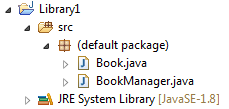
\includegraphics{library1_project.png}\hfill}

\emph{plik Book.java}

\begin{Verbatim}[commandchars=\\\{\},numbers=left,firstnumber=1,stepnumber=1]
\PYG{k+kd}{public} \PYG{k+kd}{class} \PYG{n+nc}{Book} \PYG{o}{\PYGZob{}}
    \PYG{n}{String} \PYG{n}{isbn}\PYG{o}{;}
    \PYG{n}{String} \PYG{n}{title}\PYG{o}{;}
    \PYG{n}{String} \PYG{n}{author}\PYG{o}{;}

    \PYG{n}{Book}\PYG{o}{(}\PYG{n}{String} \PYG{n}{isbn}\PYG{o}{,} \PYG{n}{String} \PYG{n}{title}\PYG{o}{,} \PYG{n}{String} \PYG{n}{author}\PYG{o}{)} \PYG{o}{\PYGZob{}}
        \PYG{k}{this}\PYG{o}{.}\PYG{n+na}{isbn} \PYG{o}{=} \PYG{n}{isbn}\PYG{o}{;}
        \PYG{k}{this}\PYG{o}{.}\PYG{n+na}{title} \PYG{o}{=} \PYG{n}{title}\PYG{o}{;}
        \PYG{k}{this}\PYG{o}{.}\PYG{n+na}{author} \PYG{o}{=} \PYG{n}{author}\PYG{o}{;}
    \PYG{o}{\PYGZcb{}}

    \PYG{n}{String} \PYG{n+nf}{getBookInfo}\PYG{o}{(}\PYG{o}{)} \PYG{o}{\PYGZob{}}
        \PYG{k}{return} \PYG{n}{isbn} \PYG{o}{+} \PYG{l+s}{\PYGZdq{} \PYGZhy{} \PYGZdq{}} \PYG{o}{+} \PYG{n}{title} \PYG{o}{+} \PYG{l+s}{\PYGZdq{} \PYGZhy{} \PYGZdq{}} \PYG{o}{+} \PYG{n}{author}\PYG{o}{;}
    \PYG{o}{\PYGZcb{}}
\PYG{o}{\PYGZcb{}}
\end{Verbatim}

\emph{plik BookManager.java}

\begin{Verbatim}[commandchars=\\\{\},numbers=left,firstnumber=1,stepnumber=1]
\PYG{k+kn}{import} \PYG{n+nn}{java.util.Scanner}\PYG{o}{;}

\PYG{k+kd}{public} \PYG{k+kd}{class} \PYG{n+nc}{BookManager} \PYG{o}{\PYGZob{}}
    \PYG{k+kd}{public} \PYG{k+kd}{static} \PYG{k+kt}{void} \PYG{n+nf}{main}\PYG{o}{(}\PYG{n}{String}\PYG{o}{[}\PYG{o}{]} \PYG{n}{args}\PYG{o}{)} \PYG{o}{\PYGZob{}}
        \PYG{c+c1}{//tworzymy obiekt do odczytu danych}
        \PYG{n}{Scanner} \PYG{n}{sc} \PYG{o}{=} \PYG{k}{new} \PYG{n}{Scanner}\PYG{o}{(}\PYG{n}{System}\PYG{o}{.}\PYG{n+na}{in}\PYG{o}{)}\PYG{o}{;}

        \PYG{c+c1}{//prosimy użytkownika o podanie odpowiednich danych}
        \PYG{n}{System}\PYG{o}{.}\PYG{n+na}{out}\PYG{o}{.}\PYG{n+na}{println}\PYG{o}{(}\PYG{l+s}{\PYGZdq{}Podaj ISBN: \PYGZdq{}}\PYG{o}{)}\PYG{o}{;}
        \PYG{n}{String} \PYG{n}{isbn} \PYG{o}{=} \PYG{n}{sc}\PYG{o}{.}\PYG{n+na}{nextLine}\PYG{o}{(}\PYG{o}{)}\PYG{o}{;}
        \PYG{n}{System}\PYG{o}{.}\PYG{n+na}{out}\PYG{o}{.}\PYG{n+na}{println}\PYG{o}{(}\PYG{l+s}{\PYGZdq{}Podaj Tytuł: \PYGZdq{}}\PYG{o}{)}\PYG{o}{;}
        \PYG{n}{String} \PYG{n}{title} \PYG{o}{=} \PYG{n}{sc}\PYG{o}{.}\PYG{n+na}{nextLine}\PYG{o}{(}\PYG{o}{)}\PYG{o}{;}
        \PYG{n}{System}\PYG{o}{.}\PYG{n+na}{out}\PYG{o}{.}\PYG{n+na}{println}\PYG{o}{(}\PYG{l+s}{\PYGZdq{}Podaj autora: \PYGZdq{}}\PYG{o}{)}\PYG{o}{;}
        \PYG{n}{String} \PYG{n}{author} \PYG{o}{=} \PYG{n}{sc}\PYG{o}{.}\PYG{n+na}{nextLine}\PYG{o}{(}\PYG{o}{)}\PYG{o}{;}

        \PYG{c+c1}{//zamykamy strumień wejścia}
        \PYG{n}{sc}\PYG{o}{.}\PYG{n+na}{close}\PYG{o}{(}\PYG{o}{)}\PYG{o}{;}

        \PYG{c+c1}{//tworzymy obiekt Book i wyświetlamy informacje na ekranie}
        \PYG{n}{Book} \PYG{n}{book} \PYG{o}{=} \PYG{k}{new} \PYG{n}{Book}\PYG{o}{(}\PYG{n}{isbn}\PYG{o}{,} \PYG{n}{title}\PYG{o}{,} \PYG{n}{author}\PYG{o}{)}\PYG{o}{;}
        \PYG{n}{System}\PYG{o}{.}\PYG{n+na}{out}\PYG{o}{.}\PYG{n+na}{println}\PYG{o}{(}\PYG{n}{book}\PYG{o}{.}\PYG{n+na}{getBookInfo}\PYG{o}{(}\PYG{o}{)}\PYG{o}{)}\PYG{o}{;}
    \PYG{o}{\PYGZcb{}}
\PYG{o}{\PYGZcb{}}
\end{Verbatim}

Przykładowy wynik działania programu:

{\hfill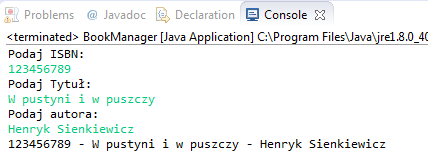
\includegraphics{output1.png}\hfill}


\subsection{Dziedziczenie}
\label{obiekty2:dziedziczenie}
W naszej aplikacji możemy teraz przechowywać i wczytywać od użytkownika informacje o książkach, jednak warto zauważyć, że przecież w bibliotece oprócz książek są także komiksy, gazety, ogólnie rzecz ujmując magazyny. W tym momencie należałoby stworzyć osobną klasę Magazine, która przechowywać będzie również numer ISBN, tytuł, oraz np. wydawnictwo. Problemem jest to, że pewne dane zaczynają się tutaj powielać, a tego w programowaniu zdecydowanie powinniśmy unikać.

W celu rozwiązania m.in. tego problemu powstał paradygmat programowania obiektowego, które pozwala budować hierarchię klas, dającą możliwość tworzenia kodu, który może być wykorzystywany wielokrotnie i być bazą do tworzenia jeszcze kolejnych klas.

{\hfill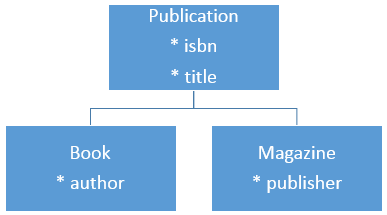
\includegraphics{inheritance.png}\hfill}

Na powyższym diagramie widać bazową klasę \textbf{Publication}, po której dziedziczą dwie kolejne klasy: \textbf{Book} oraz \textbf{Magazine}. Różnią się one tym, że książka posiada najczęściej jednego autora (np. Henryk Sienkiewicz), natomiast w przypadku gazety w tym miejscu pojawi się wydawnictwo (np. Ringier Axel Springer).

\begin{notice}{note}{Note:}
Jeżeli istnieje pewna klasa \textbf{A}, a poniej dziedziczy pewna klasa \textbf{B}, to klasa \textbf{B} przejmuje wszystkie widoczne cechy klasy \textbf{A}.
\end{notice}

Powyższa regułka oznacza, że w przypadku, gdy spojrzymy na powyższy diagram, klasa \textbf{Book}, czy \textbf{Magazine} będą posiadały także pola z klasy \textbf{Publication}, czyli \emph{isbn} oraz \emph{title}. W Javie dziedziczenie można osiągnąć stosując słowo kluczowe \textbf{extends} w definicji klasy, np.:

{\hfill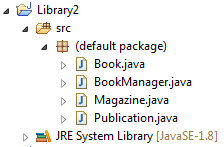
\includegraphics{inherit.png}\hfill}

\emph{plik Publication.java}

\begin{Verbatim}[commandchars=\\\{\},numbers=left,firstnumber=1,stepnumber=1]
\PYG{k+kd}{public} \PYG{k+kd}{class} \PYG{n+nc}{Publication} \PYG{o}{\PYGZob{}}
    \PYG{n}{String} \PYG{n}{isbn}\PYG{o}{;}
    \PYG{n}{String} \PYG{n}{title}\PYG{o}{;}

    \PYG{n}{Publication}\PYG{o}{(}\PYG{n}{String} \PYG{n}{isbn}\PYG{o}{,} \PYG{n}{String} \PYG{n}{title}\PYG{o}{)} \PYG{o}{\PYGZob{}}
        \PYG{k}{this}\PYG{o}{.}\PYG{n+na}{isbn} \PYG{o}{=} \PYG{n}{isbn}\PYG{o}{;}
        \PYG{k}{this}\PYG{o}{.}\PYG{n+na}{title} \PYG{o}{=} \PYG{n}{title}\PYG{o}{;}
    \PYG{o}{\PYGZcb{}}

    \PYG{n}{String} \PYG{n+nf}{getInfo}\PYG{o}{(}\PYG{o}{)} \PYG{o}{\PYGZob{}}
        \PYG{k}{return} \PYG{n}{title} \PYG{o}{+} \PYG{l+s}{\PYGZdq{} \PYGZhy{} \PYGZdq{}} \PYG{o}{+} \PYG{n}{isbn}\PYG{o}{;}
    \PYG{o}{\PYGZcb{}}
\PYG{o}{\PYGZcb{}}
\end{Verbatim}

\emph{plik Book.java}

\begin{Verbatim}[commandchars=\\\{\},numbers=left,firstnumber=1,stepnumber=1]
\PYG{k+kd}{public} \PYG{k+kd}{class} \PYG{n+nc}{Book} \PYG{k+kd}{extends} \PYG{n}{Publication} \PYG{o}{\PYGZob{}}
    \PYG{n}{String} \PYG{n}{author}\PYG{o}{;}

    \PYG{n}{Book}\PYG{o}{(}\PYG{n}{String} \PYG{n}{isbn}\PYG{o}{,} \PYG{n}{String} \PYG{n}{title}\PYG{o}{,} \PYG{n}{String} \PYG{n}{author}\PYG{o}{)} \PYG{o}{\PYGZob{}}
        \PYG{k+kd}{super}\PYG{o}{(}\PYG{n}{isbn}\PYG{o}{,} \PYG{n}{title}\PYG{o}{)}\PYG{o}{;}
        \PYG{k}{this}\PYG{o}{.}\PYG{n+na}{author} \PYG{o}{=} \PYG{n}{author}\PYG{o}{;}
    \PYG{o}{\PYGZcb{}}

    \PYG{n}{String} \PYG{n+nf}{getInfo}\PYG{o}{(}\PYG{o}{)} \PYG{o}{\PYGZob{}}
        \PYG{k}{return} \PYG{k+kd}{super}\PYG{o}{.}\PYG{n+na}{getInfo}\PYG{o}{(}\PYG{o}{)} \PYG{o}{+} \PYG{l+s}{\PYGZdq{} \PYGZhy{} \PYGZdq{}} \PYG{o}{+} \PYG{n}{author}\PYG{o}{;}
    \PYG{o}{\PYGZcb{}}
\PYG{o}{\PYGZcb{}}
\end{Verbatim}

\emph{plik Magazine.java}

\begin{Verbatim}[commandchars=\\\{\},numbers=left,firstnumber=1,stepnumber=1]
\PYG{k+kd}{public} \PYG{k+kd}{class} \PYG{n+nc}{Magazine} \PYG{k+kd}{extends} \PYG{n}{Publication} \PYG{o}{\PYGZob{}}
    \PYG{n}{String} \PYG{n}{publisher}\PYG{o}{;}

    \PYG{n}{Magazine}\PYG{o}{(}\PYG{n}{String} \PYG{n}{isbn}\PYG{o}{,} \PYG{n}{String} \PYG{n}{title}\PYG{o}{,} \PYG{n}{String} \PYG{n}{publisher}\PYG{o}{)} \PYG{o}{\PYGZob{}}
        \PYG{k+kd}{super}\PYG{o}{(}\PYG{n}{isbn}\PYG{o}{,} \PYG{n}{title}\PYG{o}{)}\PYG{o}{;}
        \PYG{k}{this}\PYG{o}{.}\PYG{n+na}{publisher} \PYG{o}{=} \PYG{n}{publisher}\PYG{o}{;}
    \PYG{o}{\PYGZcb{}}

    \PYG{n}{String} \PYG{n+nf}{getInfo}\PYG{o}{(}\PYG{o}{)} \PYG{o}{\PYGZob{}}
        \PYG{k}{return} \PYG{k+kd}{super}\PYG{o}{.}\PYG{n+na}{getInfo}\PYG{o}{(}\PYG{o}{)} \PYG{o}{+} \PYG{l+s}{\PYGZdq{} \PYGZhy{} \PYGZdq{}} \PYG{o}{+} \PYG{n}{publisher}\PYG{o}{;}
    \PYG{o}{\PYGZcb{}}
\PYG{o}{\PYGZcb{}}
\end{Verbatim}

Zwróć uwagę, że pomimo iż w klasach \emph{Book} oraz \emph{Magazine} nie zadeklarowaliśmy pól \emph{isbn} oraz \emph{title} to mamy do nich dostęp w konstruktorze, czy metodach \emph{getBookInfo()} i \emph{getMagazineInfo()}, ponieważ dziedziczą one te cechy z klasy Publication.

Kolejną nowością jest zastosowanie specjalnej konstrukcji \textbf{super()}. Działa ona w sposób podobny do słowa kluczowego \emph{this}, którego używaliśmy w przypadku, gdy posiadaliśmy kilka przeciążonych wersji konstruktora z tą różnicą, że wywołuje konstruktor nadklasy z odpowiednimi parametrami.

Ostatnia rzecz dotyczy \textbf{przesłaniania} metod. W klasie Publication zdefiniowaliśmy metodę \emph{getInfo()}. Jeżeli w klasie dziedzicząsej (Book lub Magazine) zdefiniujemy metodę o takiej samej sygnaturze, to powiemy, że przesłania ona oryginalną metodę \emph{getInfo()}. W celu wywołania metody nadklasy należy posłużyć się w takiej sytuacji zapisem \textbf{super.getInfo()}.

\begin{notice}{note}{Note:}
Pierwszą, niejawną instrukcją jaka jest wykonywana w podklasie pewnej klasy bazowej jest wywołanie konstruktora nadklasy poprzez \textbf{super()}. Jeżeli w klasie bazowej nie jest zdefiniowany konstruktor bezparametrowy to należy jawnie wywołać konstruktor z odpowiednimi argumentami poprzez zapis \textbf{super(lista\_parametrow)}. Jeżeli chcesz natomiast wywołać w którejś z metod metodę z nadklasy wykorzystaj zapis \textbf{super.nazwaMetody(parametry)}.
\end{notice}

\begin{notice}{note}{Note:}
Jeżeli chcesz zaznaczyć, że jakaś metoda jest przesłonięta możesz zastosować dodatkową adnotację \emph{@Override}. W wielu sytuacjach będzie ona automatycznie wygenerowana przez eclipse, warto więc rozumieć co oznacza.

\begin{Verbatim}[commandchars=\\\{\}]
@Override
String getInfo() \PYGZob{}
    return super.getInfo() + \PYGZdq{} \PYGZhy{} \PYGZdq{} + author;
\PYGZcb{}
\end{Verbatim}
\end{notice}
\begin{description}
\item[{\textbf{Ćwiczenie} \emph{(10 min)}}] \leavevmode
W klasie BookManager utwórz tablice do przechowywania książek oraz magazynów. W każdej tablicy utwórz przynajmniej po jednym obiekcie danego typu, a następnie wyświetl je na ekranie.

\end{description}

\emph{plik BookManager.java}

\begin{Verbatim}[commandchars=\\\{\},numbers=left,firstnumber=1,stepnumber=1]
\PYG{k+kn}{import} \PYG{n+nn}{java.util.Scanner}\PYG{o}{;}

\PYG{k+kd}{public} \PYG{k+kd}{class} \PYG{n+nc}{BookManager} \PYG{o}{\PYGZob{}}
    \PYG{k+kd}{public} \PYG{k+kd}{static} \PYG{k+kt}{void} \PYG{n+nf}{main}\PYG{o}{(}\PYG{n}{String}\PYG{o}{[}\PYG{o}{]} \PYG{n}{args}\PYG{o}{)} \PYG{o}{\PYGZob{}}
        \PYG{c+c1}{// tworzymy obiekt do odczytu danych}
        \PYG{n}{Scanner} \PYG{n}{sc} \PYG{o}{=} \PYG{k}{new} \PYG{n}{Scanner}\PYG{o}{(}\PYG{n}{System}\PYG{o}{.}\PYG{n+na}{in}\PYG{o}{)}\PYG{o}{;}

        \PYG{c+c1}{// tworzymy tablice}
        \PYG{n}{Book}\PYG{o}{[}\PYG{o}{]} \PYG{n}{books} \PYG{o}{=} \PYG{k}{new} \PYG{n}{Book}\PYG{o}{[}\PYG{l+m+mi}{10}\PYG{o}{]}\PYG{o}{;}
        \PYG{n}{Magazine}\PYG{o}{[}\PYG{o}{]} \PYG{n}{magazines} \PYG{o}{=} \PYG{k}{new} \PYG{n}{Magazine}\PYG{o}{[}\PYG{l+m+mi}{10}\PYG{o}{]}\PYG{o}{;}

        \PYG{c+c1}{// prosimy użytkownika o podanie informacji o książce}
        \PYG{n}{System}\PYG{o}{.}\PYG{n+na}{out}\PYG{o}{.}\PYG{n+na}{println}\PYG{o}{(}\PYG{l+s}{\PYGZdq{}Podaj ISBN książki: \PYGZdq{}}\PYG{o}{)}\PYG{o}{;}
        \PYG{n}{String} \PYG{n}{isbn} \PYG{o}{=} \PYG{n}{sc}\PYG{o}{.}\PYG{n+na}{nextLine}\PYG{o}{(}\PYG{o}{)}\PYG{o}{;}
        \PYG{n}{System}\PYG{o}{.}\PYG{n+na}{out}\PYG{o}{.}\PYG{n+na}{println}\PYG{o}{(}\PYG{l+s}{\PYGZdq{}Podaj Tytuł książi: \PYGZdq{}}\PYG{o}{)}\PYG{o}{;}
        \PYG{n}{String} \PYG{n}{title} \PYG{o}{=} \PYG{n}{sc}\PYG{o}{.}\PYG{n+na}{nextLine}\PYG{o}{(}\PYG{o}{)}\PYG{o}{;}
        \PYG{n}{System}\PYG{o}{.}\PYG{n+na}{out}\PYG{o}{.}\PYG{n+na}{println}\PYG{o}{(}\PYG{l+s}{\PYGZdq{}Podaj autora książki: \PYGZdq{}}\PYG{o}{)}\PYG{o}{;}
        \PYG{n}{String} \PYG{n}{author} \PYG{o}{=} \PYG{n}{sc}\PYG{o}{.}\PYG{n+na}{nextLine}\PYG{o}{(}\PYG{o}{)}\PYG{o}{;}

        \PYG{n}{books}\PYG{o}{[}\PYG{l+m+mi}{0}\PYG{o}{]} \PYG{o}{=} \PYG{k}{new} \PYG{n}{Book}\PYG{o}{(}\PYG{n}{isbn}\PYG{o}{,} \PYG{n}{title}\PYG{o}{,} \PYG{n}{author}\PYG{o}{)}\PYG{o}{;}

        \PYG{c+c1}{// prosimy użytkownika o podanie informacji o magazynie}
        \PYG{n}{System}\PYG{o}{.}\PYG{n+na}{out}\PYG{o}{.}\PYG{n+na}{println}\PYG{o}{(}\PYG{l+s}{\PYGZdq{}Podaj ISBN magazynu: \PYGZdq{}}\PYG{o}{)}\PYG{o}{;}
        \PYG{n}{isbn} \PYG{o}{=} \PYG{n}{sc}\PYG{o}{.}\PYG{n+na}{nextLine}\PYG{o}{(}\PYG{o}{)}\PYG{o}{;}
        \PYG{n}{System}\PYG{o}{.}\PYG{n+na}{out}\PYG{o}{.}\PYG{n+na}{println}\PYG{o}{(}\PYG{l+s}{\PYGZdq{}Podaj Tytuł magazynu: \PYGZdq{}}\PYG{o}{)}\PYG{o}{;}
        \PYG{n}{title} \PYG{o}{=} \PYG{n}{sc}\PYG{o}{.}\PYG{n+na}{nextLine}\PYG{o}{(}\PYG{o}{)}\PYG{o}{;}
        \PYG{n}{System}\PYG{o}{.}\PYG{n+na}{out}\PYG{o}{.}\PYG{n+na}{println}\PYG{o}{(}\PYG{l+s}{\PYGZdq{}Podaj wydawcę magazynu: \PYGZdq{}}\PYG{o}{)}\PYG{o}{;}
        \PYG{n}{String} \PYG{n}{publisher} \PYG{o}{=} \PYG{n}{sc}\PYG{o}{.}\PYG{n+na}{nextLine}\PYG{o}{(}\PYG{o}{)}\PYG{o}{;}

        \PYG{n}{magazines}\PYG{o}{[}\PYG{l+m+mi}{0}\PYG{o}{]} \PYG{o}{=} \PYG{k}{new} \PYG{n}{Magazine}\PYG{o}{(}\PYG{n}{isbn}\PYG{o}{,} \PYG{n}{title}\PYG{o}{,} \PYG{n}{publisher}\PYG{o}{)}\PYG{o}{;}

        \PYG{c+c1}{// zamykamy strumień wejścia}
        \PYG{n}{sc}\PYG{o}{.}\PYG{n+na}{close}\PYG{o}{(}\PYG{o}{)}\PYG{o}{;}

        \PYG{c+c1}{// tworzymy obiekt Book i wyświetlamy informacje na ekranie}
        \PYG{n}{System}\PYG{o}{.}\PYG{n+na}{out}\PYG{o}{.}\PYG{n+na}{println}\PYG{o}{(}\PYG{n}{books}\PYG{o}{[}\PYG{l+m+mi}{0}\PYG{o}{]}\PYG{o}{.}\PYG{n+na}{getInfo}\PYG{o}{(}\PYG{o}{)}\PYG{o}{)}\PYG{o}{;}
        \PYG{n}{System}\PYG{o}{.}\PYG{n+na}{out}\PYG{o}{.}\PYG{n+na}{println}\PYG{o}{(}\PYG{n}{magazines}\PYG{o}{[}\PYG{l+m+mi}{0}\PYG{o}{]}\PYG{o}{.}\PYG{n+na}{getInfo}\PYG{o}{(}\PYG{o}{)}\PYG{o}{)}\PYG{o}{;}
    \PYG{o}{\PYGZcb{}}
\PYG{o}{\PYGZcb{}}
\end{Verbatim}

W porównaniu do wcześniejszego kodu zyskaliśmy teraz możliwosć przechowywania informacji zarówno o ksiażkach jak i innego rodzaju publikacjach. Ponieważ przechowujemy je w tablicach to dodatkowo dane są teraz bardziej spójne.


\subsection{Polimorfizm}
\label{obiekty2:polimorfizm}
Wcześniej wspomnieliśmy, że dziedziczenia warto używać między innymi po to, żeby zaoszczędzić konieczności powielania tego samego kodu. Problem w tym, że gdy tak jak w powyższym przykładzie stosujemy tablice oddzielnych typów to operacje na nich i tak będą powielane, np:

\begin{Verbatim}[commandchars=\\\{\}]
System.out.println(\PYGZdq{}Książki: \PYGZdq{});
for(int i=0; i \PYGZlt{} books.length; i++) \PYGZob{}
    if(books[1] != null)
        System.out.println(books[i].getInfo());
\PYGZcb{}

System.out.println(\PYGZdq{}Magazyny: \PYGZdq{});
for(int i=0; i \PYGZlt{} magazines.length; i++) \PYGZob{}
    if(magazines[1] != null)
        System.out.println(magazines[i].getInfo());
\PYGZcb{}
\end{Verbatim}

Lepiej by było tak naprawdę przechowywać wszystkie te dane w jednej wspólnej tablicy typu \emph{Publication}, a następnie ewentualnie rozpoznać, czy dany element tablicy jest typu Book, czy Magazine.

Efekt taki można osiągnąć dzięki zastosowaniu \textbf{polimorfizmu} lub inaczej mówiąc wielopostaciowości. Polega to na tym, że do ogólnej, wspólnej referencji można przypisać obiekty różnych typów, które po typie tej referencji dziedziczą.

W naszym przypadku klasy Book i Magazine dziedziczą po klasie Publication, więc jak najbardziej możliwe jest zapisanie:

\begin{Verbatim}[commandchars=\\\{\}]
Publication pub1 = new Book(argumenty\PYGZus{}konstruktora);
Publication pub2 = new Magazine(argumenty\PYGZus{}konstruktora);
\end{Verbatim}

W podobny sposób możemy także utworzyć tablicę typu Publication, która będzie przechowywała zarówno książki jak i magazyny. Pamiętać należy jednak o dwóch rzeczach:

1. Zawsze mamy dostęp jedynie do metod z typu referencji. Jeżeli w klasie Book zdefiniujemy dodatkową metodę changeBookTitle(), a referencja będzie typu Publication, to nie będziemy mieli dostępu do takiej metody. Jeśżeli chcesz uzyskać dostęp do wszystkich metod (również tych nie zdefiniowanych w typie nadrzędnym) musisz skorzystać z rzutowania typu. Rzutowanie polega na wykorzystaniu nawiasu, np.:

\begin{Verbatim}[commandchars=\\\{\}]
Publication pub = new Magazine(...);
((Magazine)pub).metodaZKlasyMagazine();
\end{Verbatim}
\begin{enumerate}
\setcounter{enumi}{1}
\item {} 
Metody będą wywoływane na rzecz typu obiektu, a nie typu referencji. Jeżeli zapisaliśmy \emph{Publication pub1 = new Book(argumenty\_konstruktora);} to wywołując metodę pub1.getInfo() wywołamy jej wersję z klasy Book, a nie Publication.

\end{enumerate}

\textbf{Ćwiczenie} \emph{(5 min)}
\begin{quote}

Przerób klasę BookManager w taki sposób, aby przechowywać książki oraz magazyny w jednej wspólnej tablicy typu Publication{[}{]}.
\end{quote}

\emph{plik BookManager.java}

\begin{Verbatim}[commandchars=\\\{\},numbers=left,firstnumber=1,stepnumber=1]
\PYG{k+kn}{import} \PYG{n+nn}{java.util.Scanner}\PYG{o}{;}

\PYG{k+kn}{import} \PYG{n+nn}{java.util.Scanner}\PYG{o}{;}

\PYG{k+kd}{public} \PYG{k+kd}{class} \PYG{n+nc}{BookManager} \PYG{o}{\PYGZob{}}
    \PYG{k+kd}{public} \PYG{k+kd}{static} \PYG{k+kt}{void} \PYG{n+nf}{main}\PYG{o}{(}\PYG{n}{String}\PYG{o}{[}\PYG{o}{]} \PYG{n}{args}\PYG{o}{)} \PYG{o}{\PYGZob{}}
        \PYG{c+c1}{// tworzymy obiekt do odczytu danych}
        \PYG{n}{Scanner} \PYG{n}{sc} \PYG{o}{=} \PYG{k}{new} \PYG{n}{Scanner}\PYG{o}{(}\PYG{n}{System}\PYG{o}{.}\PYG{n+na}{in}\PYG{o}{)}\PYG{o}{;}

        \PYG{c+c1}{// tworzymy tablice}
        \PYG{n}{Publication}\PYG{o}{[}\PYG{o}{]} \PYG{n}{publications} \PYG{o}{=} \PYG{k}{new} \PYG{n}{Publication}\PYG{o}{[}\PYG{l+m+mi}{10}\PYG{o}{]}\PYG{o}{;}

        \PYG{c+c1}{// prosimy użytkownika o podanie informacji o książce}
        \PYG{n}{System}\PYG{o}{.}\PYG{n+na}{out}\PYG{o}{.}\PYG{n+na}{println}\PYG{o}{(}\PYG{l+s}{\PYGZdq{}Podaj ISBN książki: \PYGZdq{}}\PYG{o}{)}\PYG{o}{;}
        \PYG{n}{String} \PYG{n}{isbn} \PYG{o}{=} \PYG{n}{sc}\PYG{o}{.}\PYG{n+na}{nextLine}\PYG{o}{(}\PYG{o}{)}\PYG{o}{;}
        \PYG{n}{System}\PYG{o}{.}\PYG{n+na}{out}\PYG{o}{.}\PYG{n+na}{println}\PYG{o}{(}\PYG{l+s}{\PYGZdq{}Podaj Tytuł książi: \PYGZdq{}}\PYG{o}{)}\PYG{o}{;}
        \PYG{n}{String} \PYG{n}{title} \PYG{o}{=} \PYG{n}{sc}\PYG{o}{.}\PYG{n+na}{nextLine}\PYG{o}{(}\PYG{o}{)}\PYG{o}{;}
        \PYG{n}{System}\PYG{o}{.}\PYG{n+na}{out}\PYG{o}{.}\PYG{n+na}{println}\PYG{o}{(}\PYG{l+s}{\PYGZdq{}Podaj autora książki: \PYGZdq{}}\PYG{o}{)}\PYG{o}{;}
        \PYG{n}{String} \PYG{n}{author} \PYG{o}{=} \PYG{n}{sc}\PYG{o}{.}\PYG{n+na}{nextLine}\PYG{o}{(}\PYG{o}{)}\PYG{o}{;}

        \PYG{n}{publications}\PYG{o}{[}\PYG{l+m+mi}{0}\PYG{o}{]} \PYG{o}{=} \PYG{k}{new} \PYG{n}{Book}\PYG{o}{(}\PYG{n}{isbn}\PYG{o}{,} \PYG{n}{title}\PYG{o}{,} \PYG{n}{author}\PYG{o}{)}\PYG{o}{;}

        \PYG{c+c1}{// prosimy użytkownika o podanie informacji o magazynie}
        \PYG{n}{System}\PYG{o}{.}\PYG{n+na}{out}\PYG{o}{.}\PYG{n+na}{println}\PYG{o}{(}\PYG{l+s}{\PYGZdq{}Podaj ISBN magazynu: \PYGZdq{}}\PYG{o}{)}\PYG{o}{;}
        \PYG{n}{isbn} \PYG{o}{=} \PYG{n}{sc}\PYG{o}{.}\PYG{n+na}{nextLine}\PYG{o}{(}\PYG{o}{)}\PYG{o}{;}
        \PYG{n}{System}\PYG{o}{.}\PYG{n+na}{out}\PYG{o}{.}\PYG{n+na}{println}\PYG{o}{(}\PYG{l+s}{\PYGZdq{}Podaj Tytuł magazynu: \PYGZdq{}}\PYG{o}{)}\PYG{o}{;}
        \PYG{n}{title} \PYG{o}{=} \PYG{n}{sc}\PYG{o}{.}\PYG{n+na}{nextLine}\PYG{o}{(}\PYG{o}{)}\PYG{o}{;}
        \PYG{n}{System}\PYG{o}{.}\PYG{n+na}{out}\PYG{o}{.}\PYG{n+na}{println}\PYG{o}{(}\PYG{l+s}{\PYGZdq{}Podaj wydawcę magazynu: \PYGZdq{}}\PYG{o}{)}\PYG{o}{;}
        \PYG{n}{String} \PYG{n}{publisher} \PYG{o}{=} \PYG{n}{sc}\PYG{o}{.}\PYG{n+na}{nextLine}\PYG{o}{(}\PYG{o}{)}\PYG{o}{;}

        \PYG{n}{publications}\PYG{o}{[}\PYG{l+m+mi}{1}\PYG{o}{]} \PYG{o}{=} \PYG{k}{new} \PYG{n}{Magazine}\PYG{o}{(}\PYG{n}{isbn}\PYG{o}{,} \PYG{n}{title}\PYG{o}{,} \PYG{n}{publisher}\PYG{o}{)}\PYG{o}{;}

        \PYG{c+c1}{// zamykamy strumień wejścia}
        \PYG{n}{sc}\PYG{o}{.}\PYG{n+na}{close}\PYG{o}{(}\PYG{o}{)}\PYG{o}{;}

        \PYG{c+c1}{// wyświetlamy informacje na ekranie}
        \PYG{n}{System}\PYG{o}{.}\PYG{n+na}{out}\PYG{o}{.}\PYG{n+na}{println}\PYG{o}{(}\PYG{l+s}{\PYGZdq{}Książki i magazyny: \PYGZdq{}}\PYG{o}{)}\PYG{o}{;}
        \PYG{k}{for} \PYG{o}{(}\PYG{n}{Publication} \PYG{n+nl}{p:} \PYG{n}{publications}\PYG{o}{)} \PYG{o}{\PYGZob{}}
            \PYG{k}{if} \PYG{o}{(}\PYG{n}{p} \PYG{o}{!}\PYG{o}{=} \PYG{k+kc}{null}\PYG{o}{)}
                \PYG{n}{System}\PYG{o}{.}\PYG{n+na}{out}\PYG{o}{.}\PYG{n+na}{println}\PYG{o}{(}\PYG{n}{p}\PYG{o}{.}\PYG{n+na}{getInfo}\PYG{o}{(}\PYG{o}{)}\PYG{o}{)}\PYG{o}{;}
        \PYG{o}{\PYGZcb{}}
    \PYG{o}{\PYGZcb{}}
\PYG{o}{\PYGZcb{}}
\end{Verbatim}

Dzięki uproszczeniu sposobu przechowywania danych wyświetlanie danych odbywa się w jednej tylko pętli, dane są bardziej spójne, a kod bardziej przejrzysty.


\subsection{Operator instanceof}
\label{obiekty2:operator-instanceof}
W poprzednim przykładzie brakuje w tej chwili trochę informacji o tym, czy dana pozycja w tablicy \emph{publications} jest typu Book, czy Magazine. W niektórych sytuacjach chcielibyśmy mieć taką informację w celu zwiększenia przejrzystości. W Javie możemy sprawdzić rzeczywisty typ obiektu (nie typ referencji) za pomocą operatora \textbf{instanceof}. Jego składnia jest następująca:

\begin{Verbatim}[commandchars=\\\{\}]
\PYG{n}{obiekt} \PYG{k}{instanceof} \PYG{n}{NazwaKlasy}
\end{Verbatim}

np.

\begin{Verbatim}[commandchars=\\\{\}]
\PYG{n}{Publication} \PYG{n}{book} \PYG{o}{=} \PYG{k}{new} \PYG{n}{Book}\PYG{o}{(}\PYG{l+s}{\PYGZdq{}123456789\PYGZdq{}}\PYG{o}{,} \PYG{l+s}{\PYGZdq{}W pustyni i w puszczy\PYGZdq{}}\PYG{o}{,} \PYG{l+s}{\PYGZdq{}Henryk Sienkiewicz\PYGZdq{}}\PYG{o}{)}\PYG{o}{;}
\PYG{k}{if}\PYG{o}{(}\PYG{n}{book} \PYG{k}{instanceof} \PYG{n}{Book}\PYG{o}{)} \PYG{o}{\PYGZob{}}
    \PYG{n}{System}\PYG{o}{.}\PYG{n+na}{out}\PYG{o}{.}\PYG{n+na}{println}\PYG{o}{(}\PYG{l+s}{\PYGZdq{}To jest książka\PYGZdq{}}\PYG{o}{)}\PYG{o}{;}
\PYG{o}{\PYGZcb{}}
\end{Verbatim}

Na ekranie zobaczymy tekst ``To jest ksiażka''.

Sprawdzenie obiektu za pomocą operatora instanceof zwraca w wyniku true lub false, więc jak widać w powyższym przykładzie, może on być zastosowany jako warunek w instrukcji if.

\textbf{Ćwiczenie} \emph{(5 min)}
\begin{quote}

Przerób kod klasy BookManager w taki sposób, aby dane były wyświetlane w formie:

\begin{Verbatim}[commandchars=\\\{\}]
Książka: 123456789 \PYGZhy{} W pustyni i w puszczy \PYGZhy{} Henryk Sienkiewicz
Magazyn: 987654321 \PYGZhy{} Wprost \PYGZhy{} Wydawnictwo Wprost
\end{Verbatim}
\end{quote}

\emph{plik BookManager.java}

\begin{Verbatim}[commandchars=\\\{\},numbers=left,firstnumber=1,stepnumber=1]
\PYG{k+kn}{import} \PYG{n+nn}{java.util.Scanner}\PYG{o}{;}

\PYG{k+kd}{public} \PYG{k+kd}{class} \PYG{n+nc}{BookManager} \PYG{o}{\PYGZob{}}
    \PYG{k+kd}{public} \PYG{k+kd}{static} \PYG{k+kt}{void} \PYG{n+nf}{main}\PYG{o}{(}\PYG{n}{String}\PYG{o}{[}\PYG{o}{]} \PYG{n}{args}\PYG{o}{)} \PYG{o}{\PYGZob{}}
        \PYG{c+c1}{// tworzymy obiekt do odczytu danych}
        \PYG{n}{Scanner} \PYG{n}{sc} \PYG{o}{=} \PYG{k}{new} \PYG{n}{Scanner}\PYG{o}{(}\PYG{n}{System}\PYG{o}{.}\PYG{n+na}{in}\PYG{o}{)}\PYG{o}{;}

        \PYG{c+c1}{// tworzymy tablice}
        \PYG{n}{Publication}\PYG{o}{[}\PYG{o}{]} \PYG{n}{publications} \PYG{o}{=} \PYG{k}{new} \PYG{n}{Publication}\PYG{o}{[}\PYG{l+m+mi}{10}\PYG{o}{]}\PYG{o}{;}

        \PYG{c+c1}{// prosimy użytkownika o podanie informacji o książce}
        \PYG{n}{System}\PYG{o}{.}\PYG{n+na}{out}\PYG{o}{.}\PYG{n+na}{println}\PYG{o}{(}\PYG{l+s}{\PYGZdq{}Podaj ISBN książki: \PYGZdq{}}\PYG{o}{)}\PYG{o}{;}
        \PYG{n}{String} \PYG{n}{isbn} \PYG{o}{=} \PYG{n}{sc}\PYG{o}{.}\PYG{n+na}{nextLine}\PYG{o}{(}\PYG{o}{)}\PYG{o}{;}
        \PYG{n}{System}\PYG{o}{.}\PYG{n+na}{out}\PYG{o}{.}\PYG{n+na}{println}\PYG{o}{(}\PYG{l+s}{\PYGZdq{}Podaj Tytuł książi: \PYGZdq{}}\PYG{o}{)}\PYG{o}{;}
        \PYG{n}{String} \PYG{n}{title} \PYG{o}{=} \PYG{n}{sc}\PYG{o}{.}\PYG{n+na}{nextLine}\PYG{o}{(}\PYG{o}{)}\PYG{o}{;}
        \PYG{n}{System}\PYG{o}{.}\PYG{n+na}{out}\PYG{o}{.}\PYG{n+na}{println}\PYG{o}{(}\PYG{l+s}{\PYGZdq{}Podaj autora książki: \PYGZdq{}}\PYG{o}{)}\PYG{o}{;}
        \PYG{n}{String} \PYG{n}{author} \PYG{o}{=} \PYG{n}{sc}\PYG{o}{.}\PYG{n+na}{nextLine}\PYG{o}{(}\PYG{o}{)}\PYG{o}{;}

        \PYG{n}{publications}\PYG{o}{[}\PYG{l+m+mi}{0}\PYG{o}{]} \PYG{o}{=} \PYG{k}{new} \PYG{n}{Book}\PYG{o}{(}\PYG{n}{isbn}\PYG{o}{,} \PYG{n}{title}\PYG{o}{,} \PYG{n}{author}\PYG{o}{)}\PYG{o}{;}

        \PYG{c+c1}{// prosimy użytkownika o podanie informacji o magazynie}
        \PYG{n}{System}\PYG{o}{.}\PYG{n+na}{out}\PYG{o}{.}\PYG{n+na}{println}\PYG{o}{(}\PYG{l+s}{\PYGZdq{}Podaj ISBN magazynu: \PYGZdq{}}\PYG{o}{)}\PYG{o}{;}
        \PYG{n}{isbn} \PYG{o}{=} \PYG{n}{sc}\PYG{o}{.}\PYG{n+na}{nextLine}\PYG{o}{(}\PYG{o}{)}\PYG{o}{;}
        \PYG{n}{System}\PYG{o}{.}\PYG{n+na}{out}\PYG{o}{.}\PYG{n+na}{println}\PYG{o}{(}\PYG{l+s}{\PYGZdq{}Podaj Tytuł magazynu: \PYGZdq{}}\PYG{o}{)}\PYG{o}{;}
        \PYG{n}{title} \PYG{o}{=} \PYG{n}{sc}\PYG{o}{.}\PYG{n+na}{nextLine}\PYG{o}{(}\PYG{o}{)}\PYG{o}{;}
        \PYG{n}{System}\PYG{o}{.}\PYG{n+na}{out}\PYG{o}{.}\PYG{n+na}{println}\PYG{o}{(}\PYG{l+s}{\PYGZdq{}Podaj wydawcę magazynu: \PYGZdq{}}\PYG{o}{)}\PYG{o}{;}
        \PYG{n}{String} \PYG{n}{publisher} \PYG{o}{=} \PYG{n}{sc}\PYG{o}{.}\PYG{n+na}{nextLine}\PYG{o}{(}\PYG{o}{)}\PYG{o}{;}

        \PYG{n}{publications}\PYG{o}{[}\PYG{l+m+mi}{1}\PYG{o}{]} \PYG{o}{=} \PYG{k}{new} \PYG{n}{Magazine}\PYG{o}{(}\PYG{n}{isbn}\PYG{o}{,} \PYG{n}{title}\PYG{o}{,} \PYG{n}{publisher}\PYG{o}{)}\PYG{o}{;}

        \PYG{c+c1}{// zamykamy strumień wejścia}
        \PYG{n}{sc}\PYG{o}{.}\PYG{n+na}{close}\PYG{o}{(}\PYG{o}{)}\PYG{o}{;}

        \PYG{c+c1}{// wyświetlamy informacje na ekranie}
        \PYG{n}{System}\PYG{o}{.}\PYG{n+na}{out}\PYG{o}{.}\PYG{n+na}{println}\PYG{o}{(}\PYG{l+s}{\PYGZdq{}Książki i magazyny: \PYGZdq{}}\PYG{o}{)}\PYG{o}{;}
        \PYG{k}{for} \PYG{o}{(}\PYG{n}{Publication} \PYG{n+nl}{p:} \PYG{n}{publications}\PYG{o}{)} \PYG{o}{\PYGZob{}}
            \PYG{k}{if} \PYG{o}{(}\PYG{n}{p} \PYG{o}{!}\PYG{o}{=} \PYG{k+kc}{null}\PYG{o}{)}
                \PYG{k}{if}\PYG{o}{(}\PYG{n}{p} \PYG{k}{instanceof} \PYG{n}{Book}\PYG{o}{)} \PYG{o}{\PYGZob{}}
                    \PYG{n}{System}\PYG{o}{.}\PYG{n+na}{out}\PYG{o}{.}\PYG{n+na}{println}\PYG{o}{(}\PYG{l+s}{\PYGZdq{}Książka: \PYGZdq{}} \PYG{o}{+} \PYG{n}{p}\PYG{o}{.}\PYG{n+na}{getInfo}\PYG{o}{(}\PYG{o}{)}\PYG{o}{)}\PYG{o}{;}
                \PYG{o}{\PYGZcb{}} \PYG{k}{else} \PYG{k}{if}\PYG{o}{(}\PYG{n}{p} \PYG{k}{instanceof} \PYG{n}{Magazine}\PYG{o}{)} \PYG{o}{\PYGZob{}}
                    \PYG{n}{System}\PYG{o}{.}\PYG{n+na}{out}\PYG{o}{.}\PYG{n+na}{println}\PYG{o}{(}\PYG{l+s}{\PYGZdq{}Magazyn: \PYGZdq{}} \PYG{o}{+} \PYG{n}{p}\PYG{o}{.}\PYG{n+na}{getInfo}\PYG{o}{(}\PYG{o}{)}\PYG{o}{)}\PYG{o}{;}
                \PYG{o}{\PYGZcb{}}
        \PYG{o}{\PYGZcb{}}
    \PYG{o}{\PYGZcb{}}
\PYG{o}{\PYGZcb{}}
\end{Verbatim}


\subsection{Klasy abstrakcyjne i interfejsy}
\label{obiekty2:klasy-abstrakcyjne-i-interfejsy}
Nasza aplikacja jest już prawie gotowa, jednak warto się zastanowić nad jeszcze jedną rzeczą. Stworzyliśmy klasę Publication, która jest klasą bazową dla dwóch konkretnych typów danych, które wykorzystujemy. Ponieważ nie chcemy używać obiektów klasy Publication bezpośrednio, powinniśmy z niej zrobić jedynie pewną warstwę abstrakcji, czyli klasę, która jest jedynie klasą bazową dla innych typów, ale nie można tworzyć jej obiektów bezpośrednio.

W Javie można to osiągnąć wykorzystując \textbf{klasę abstrakcyjną}. Jeżeli jakaś klasa ma być abstrakcyjna, należy w jej sygnaturze dodać o tym informację za pomocą słowa kluczowego \textbf{abstract}.

\emph{plik Publication.java}

\begin{Verbatim}[commandchars=\\\{\},numbers=left,firstnumber=1,stepnumber=1]
\PYG{k+kd}{public} \PYG{k+kd}{abstract} \PYG{k+kd}{class} \PYG{n+nc}{Publication} \PYG{o}{\PYGZob{}}
    \PYG{n}{String} \PYG{n}{isbn}\PYG{o}{;}
    \PYG{n}{String} \PYG{n}{title}\PYG{o}{;}

    \PYG{n}{Publication}\PYG{o}{(}\PYG{n}{String} \PYG{n}{isbn}\PYG{o}{,} \PYG{n}{String} \PYG{n}{title}\PYG{o}{)} \PYG{o}{\PYGZob{}}
        \PYG{k}{this}\PYG{o}{.}\PYG{n+na}{isbn} \PYG{o}{=} \PYG{n}{isbn}\PYG{o}{;}
        \PYG{k}{this}\PYG{o}{.}\PYG{n+na}{title} \PYG{o}{=} \PYG{n}{title}\PYG{o}{;}
    \PYG{o}{\PYGZcb{}}

    \PYG{n}{String} \PYG{n+nf}{getInfo}\PYG{o}{(}\PYG{o}{)} \PYG{o}{\PYGZob{}}
        \PYG{k}{return} \PYG{n}{title} \PYG{o}{+} \PYG{l+s}{\PYGZdq{} \PYGZhy{} \PYGZdq{}} \PYG{o}{+} \PYG{n}{isbn}\PYG{o}{;}
    \PYG{o}{\PYGZcb{}}
\PYG{o}{\PYGZcb{}}
\end{Verbatim}

Klasy abstrakcyjne mają dwie ważne właściwości, o których musisz pamiętać:
\begin{enumerate}
\item {} 
Nie można utworzyć obiektu klasy abstrakcyjnej za pomocą operatora new. Typ abstrakcyjny może być jedynie typem referencji dla typów bardziej sprecyzowanych (dziedziczących po tej klasie abstrakcyjnej).

\item {} 
W klasie abstrakcyjnej mogą być zdefiniowane \textbf{metody abstrakcyjne}, czyli metody, które określają jedynie sygnaturę metody, ale nie posiadają implementacji. Jeżeli jakaś klasa posiada chociaż jedną metodę abstrakcyjną, to musi być oznaczona jako klasa abstrakcyjna. Każda klasa, która dziedziczy po klasie abstrakcyjnej musi posiadać konkretną implementację każdej metody abstrakcyjnej.

\end{enumerate}

Przykład metody abstrakcyjnej:

\emph{plik Publication.java}

\begin{Verbatim}[commandchars=\\\{\},numbers=left,firstnumber=1,stepnumber=1]
\PYG{k+kd}{public} \PYG{k+kd}{abstract} \PYG{k+kd}{class} \PYG{n+nc}{Publication} \PYG{o}{\PYGZob{}}
    \PYG{n}{String} \PYG{n}{isbn}\PYG{o}{;}
    \PYG{n}{String} \PYG{n}{title}\PYG{o}{;}

    \PYG{n}{Publication}\PYG{o}{(}\PYG{n}{String} \PYG{n}{isbn}\PYG{o}{,} \PYG{n}{String} \PYG{n}{title}\PYG{o}{)} \PYG{o}{\PYGZob{}}
        \PYG{k}{this}\PYG{o}{.}\PYG{n+na}{isbn} \PYG{o}{=} \PYG{n}{isbn}\PYG{o}{;}
        \PYG{k}{this}\PYG{o}{.}\PYG{n+na}{title} \PYG{o}{=} \PYG{n}{title}\PYG{o}{;}
    \PYG{o}{\PYGZcb{}}

    \PYG{n}{String} \PYG{n+nf}{getInfo}\PYG{o}{(}\PYG{o}{)} \PYG{o}{\PYGZob{}}
        \PYG{k}{return} \PYG{n}{title} \PYG{o}{+} \PYG{l+s}{\PYGZdq{} \PYGZhy{} \PYGZdq{}} \PYG{o}{+} \PYG{n}{isbn}\PYG{o}{;}
    \PYG{o}{\PYGZcb{}}

    \PYG{k+kd}{abstract} \PYG{k+kt}{void} \PYG{n+nf}{printInfo}\PYG{o}{(}\PYG{o}{)}\PYG{o}{;}
\PYG{o}{\PYGZcb{}}
\end{Verbatim}

Jak widzisz metoda \emph{printInfo()} oznaczona jest słowek abstract. Nie posiada ona żadnej implementacji - nie posiada nawet nawiasów klamrowych i zakończona jest średnikiem.

{\hfill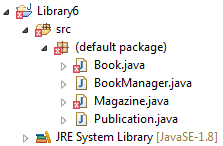
\includegraphics{abstract.png}\hfill}

Jak widzisz dodanie metody abstrakcyjnej powoduje błędy w naszym projekcie w klasach dziedziczących po Publication. W celu ich wyeliminowania powinniśmy zaimplementować metodę \emph{printInfo()} w tych klasach, np.:

\emph{plik Book.java}

\begin{Verbatim}[commandchars=\\\{\},numbers=left,firstnumber=1,stepnumber=1]
\PYG{k+kd}{public} \PYG{k+kd}{class} \PYG{n+nc}{Book} \PYG{k+kd}{extends} \PYG{n}{Publication} \PYG{o}{\PYGZob{}}
    \PYG{n}{String} \PYG{n}{author}\PYG{o}{;}

    \PYG{n}{Book}\PYG{o}{(}\PYG{n}{String} \PYG{n}{isbn}\PYG{o}{,} \PYG{n}{String} \PYG{n}{title}\PYG{o}{,} \PYG{n}{String} \PYG{n}{author}\PYG{o}{)} \PYG{o}{\PYGZob{}}
        \PYG{k+kd}{super}\PYG{o}{(}\PYG{n}{isbn}\PYG{o}{,} \PYG{n}{title}\PYG{o}{)}\PYG{o}{;}
        \PYG{k}{this}\PYG{o}{.}\PYG{n+na}{author} \PYG{o}{=} \PYG{n}{author}\PYG{o}{;}
    \PYG{o}{\PYGZcb{}}

    \PYG{n}{String} \PYG{n+nf}{getInfo}\PYG{o}{(}\PYG{o}{)} \PYG{o}{\PYGZob{}}
        \PYG{k}{return} \PYG{k+kd}{super}\PYG{o}{.}\PYG{n+na}{getInfo}\PYG{o}{(}\PYG{o}{)} \PYG{o}{+} \PYG{l+s}{\PYGZdq{} \PYGZhy{} \PYGZdq{}} \PYG{o}{+} \PYG{n}{author}\PYG{o}{;}
    \PYG{o}{\PYGZcb{}}

    \PYG{n+nd}{@Override}
    \PYG{k+kt}{void} \PYG{n+nf}{printInfo}\PYG{o}{(}\PYG{o}{)} \PYG{o}{\PYGZob{}}
        \PYG{n}{System}\PYG{o}{.}\PYG{n+na}{out}\PYG{o}{.}\PYG{n+na}{println}\PYG{o}{(}\PYG{n}{getInfo}\PYG{o}{(}\PYG{o}{)}\PYG{o}{)}\PYG{o}{;}
    \PYG{o}{\PYGZcb{}}
\PYG{o}{\PYGZcb{}}
\end{Verbatim}

analogicznie w klasie Magazine:

\emph{plik Magazine.java}

\begin{Verbatim}[commandchars=\\\{\},numbers=left,firstnumber=1,stepnumber=1]
\PYG{k+kd}{public} \PYG{k+kd}{class} \PYG{n+nc}{Magazine} \PYG{k+kd}{extends} \PYG{n}{Publication} \PYG{o}{\PYGZob{}}
    \PYG{n}{String} \PYG{n}{publisher}\PYG{o}{;}

    \PYG{n}{Magazine}\PYG{o}{(}\PYG{n}{String} \PYG{n}{isbn}\PYG{o}{,} \PYG{n}{String} \PYG{n}{title}\PYG{o}{,} \PYG{n}{String} \PYG{n}{publisher}\PYG{o}{)} \PYG{o}{\PYGZob{}}
        \PYG{k+kd}{super}\PYG{o}{(}\PYG{n}{isbn}\PYG{o}{,} \PYG{n}{title}\PYG{o}{)}\PYG{o}{;}
        \PYG{k}{this}\PYG{o}{.}\PYG{n+na}{publisher} \PYG{o}{=} \PYG{n}{publisher}\PYG{o}{;}
    \PYG{o}{\PYGZcb{}}

    \PYG{n}{String} \PYG{n+nf}{getInfo}\PYG{o}{(}\PYG{o}{)} \PYG{o}{\PYGZob{}}
        \PYG{k}{return} \PYG{k+kd}{super}\PYG{o}{.}\PYG{n+na}{getInfo}\PYG{o}{(}\PYG{o}{)} \PYG{o}{+} \PYG{l+s}{\PYGZdq{} \PYGZhy{} \PYGZdq{}} \PYG{o}{+} \PYG{n}{publisher}\PYG{o}{;}
    \PYG{o}{\PYGZcb{}}

    \PYG{n+nd}{@Override}
    \PYG{k+kt}{void} \PYG{n+nf}{printInfo}\PYG{o}{(}\PYG{o}{)} \PYG{o}{\PYGZob{}}
        \PYG{n}{System}\PYG{o}{.}\PYG{n+na}{out}\PYG{o}{.}\PYG{n+na}{println}\PYG{o}{(}\PYG{n}{getInfo}\PYG{o}{(}\PYG{o}{)}\PYG{o}{)}\PYG{o}{;}
    \PYG{o}{\PYGZcb{}}
\PYG{o}{\PYGZcb{}}
\end{Verbatim}

W Javie istnieją także klasy, które są w pełni abstrakcyjne nazywane \textbf{interfejsami}, czyli posiadają jedynie metody abstrakcyjne oraz ewentualnie zdefiniowane stałe wartości (oznaczone jako public static). Interfejsy definiujemy za pomocą słowa kluczowego \textbf{interface}, a implementujemy je (analogia do dziedziczenia) za pomocą słowa kluczowego \textbf{implements}. Na tym etapie nie będziemy się zagłębiali w stosowanie interfejsów w swoich programach, spójrz jedynie na przykład i zapamiętaj kilka rzeczy zapisanych poniżej.

Przykład interfejsu:

\begin{Verbatim}[commandchars=\\\{\},numbers=left,firstnumber=1,stepnumber=1]
\PYG{k+kd}{public} \PYG{k+kd}{interface} \PYG{n+nc}{Moveable} \PYG{o}{\PYGZob{}}
    \PYG{k+kt}{void} \PYG{n+nf}{move}\PYG{o}{(}\PYG{o}{)}\PYG{o}{;}

    \PYG{k+kt}{void} \PYG{n+nf}{stop}\PYG{o}{(}\PYG{o}{)}\PYG{o}{;}
\PYG{o}{\PYGZcb{}}
\end{Verbatim}

Klasa implementująca interfejs Moveable:

\begin{Verbatim}[commandchars=\\\{\},numbers=left,firstnumber=1,stepnumber=1]
\PYG{k+kd}{public} \PYG{k+kd}{class} \PYG{n+nc}{Car} \PYG{k+kd}{implements} \PYG{n}{Moveable} \PYG{o}{\PYGZob{}}

    \PYG{k+kd}{public} \PYG{k+kt}{void} \PYG{n+nf}{move}\PYG{o}{(}\PYG{o}{)} \PYG{o}{\PYGZob{}}
        \PYG{n}{System}\PYG{o}{.}\PYG{n+na}{out}\PYG{o}{.}\PYG{n+na}{println}\PYG{o}{(}\PYG{l+s}{\PYGZdq{}Samochód start\PYGZdq{}}\PYG{o}{)}\PYG{o}{;}
    \PYG{o}{\PYGZcb{}}

    \PYG{k+kd}{public} \PYG{k+kt}{void} \PYG{n+nf}{stop}\PYG{o}{(}\PYG{o}{)} \PYG{o}{\PYGZob{}}
        \PYG{n}{System}\PYG{o}{.}\PYG{n+na}{out}\PYG{o}{.}\PYG{n+na}{println}\PYG{o}{(}\PYG{l+s}{\PYGZdq{}Samochód stop\PYGZdq{}}\PYG{o}{)}\PYG{o}{;}
    \PYG{o}{\PYGZcb{}}
\PYG{o}{\PYGZcb{}}
\end{Verbatim}

Ponieważ wszystkie metody interfejsu muszą być abstrakcyjne, to nie jest konieczne jawne używanie słowa kluczowego abstract - jest ono niejawnie dodawane automatycznie.

\textbf{Zapamiętaj}
\begin{enumerate}
\item {} 
W Javie można dziedziczyć tylko po jednej klasie (extends), nawet jeśli są to klasy abstrakcyjne.

\item {} 
Możesz implementować dowolną liczbę interfejsów (implements).

\end{enumerate}


\subsection{Dodatek - składowe statyczne}
\label{obiekty2:dodatek-skladowe-statyczne}
Jako dodatek tej lekcji wytłumaczymy jescze krótko co oznacza słowo kluczowe \textbf{static}. W niektorych sytuacjach chcielibyśmy mieć dostęp do metody, czy pola klasy bez konieczności tworzenia obiektu. Przykładem takiej metody jest dobrze nam już znana metoda \emph{main()}.

Jeżeli zdefiniujemy jakieś pole lub metodę jako statyczne, to możemy się do nich odwoływać bez tworzenia obiektu takiej klasy poprzez konstrukcję NazwaKlasy.nazwaPolaStatycznego lub NazwaKlasy.metodaStatyczna().

Najważniejszą rzeczą dotyczącą składowych statycznych klasy jest to, że w metodach statycznych możemy odwoływać się jedynie do innych elementów statycznych tej klasy.


\section{Wyjątki i kolekcje}
\label{wyjkol:wyjatki-i-kolekcje}\label{wyjkol::doc}
W tej lekcji dowiesz się:
\begin{itemize}
\item {} 
Czym są wyjątki i jak je obsługiwać

\item {} 
Czym są kolekcje (listy, zbiory i mapy)

\item {} 
Co to oznacza, że kolekcje są typem generycznym

\item {} 
Jakie są typy opakowujące

\item {} 
Co oznaczają pojęcia autoboxing i unboxing

\end{itemize}


\subsection{Wyjątki}
\label{wyjkol:wyjatki}
W każdym programie występują pewne sytuacje wyjątkowe, które jednak można przewidzieć i w odpowiedni sposób obsłużyć. Nasza aplikacja powinna być odporna przede wszystkim na błędy, które mogą wyniknąć nie z naszej programistycznej winy, czyli np. zamknięcie połączenia sieciowego w trakcie komunikacji z innym komputerem podłączonym do sieci, błąd odczytu pliku, albo zwyczajnie wprowadzenie przez użytkownika danych w niepoprawnym formacie (napis zamiast liczby).

We wszystkich takich przypadkach zostają wygenerowane wyjątki, czyli specjalne obiekty, które mówią o tym co poszło nie tak jak powinno. W Javie istnieją dwa sposoby na obsługę wyjątków, które w tym miejscu krótko omówimy.

Hierarchia dziedziczenia klas wyjątków wygląda tak jak na poniższym schemacie.

{\hfill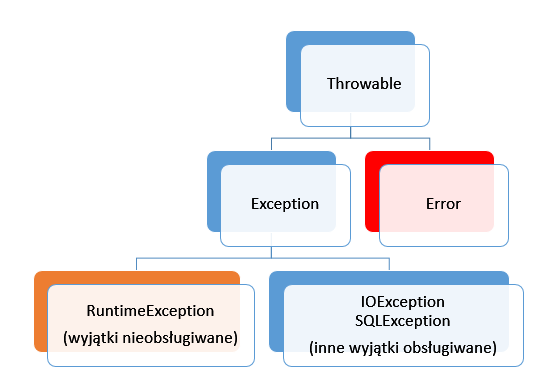
\includegraphics{exception-hierarchy.png}\hfill}

Nie musisz tego zapamiętywać, ponieważ najważniejszą różnicą pomiędzy poszczególnymi typami wyjątków jest to, czy musimy je obsługiwać, czy też nie. Obsługę wyjątków w niektórych sytuacjach wymusi na Tobie eclipse. W innych sytuacjach warto spojrzeć na sygnatury metod w dokumentacji, ponieważ to w nich znajdziesz informację, czy może ona generować jakiś wyjątek.

Zacznijmy od prostej aplikacji, która posłuży nam do omówienia zagadnień tej lekcji.

\textbf{Ćwiczenie} \emph{(10 minut)}
\begin{quote}

Przeanalizuj kod poniższego programu, który służy do zbierania danych o uczestnikach dowolnego konkursu, uruchom go oraz przetestuj dostępne opcje.
\end{quote}

{\hfill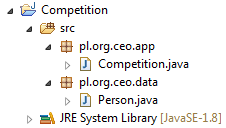
\includegraphics{comp.png}\hfill}

\emph{plik Person.java}

\begin{Verbatim}[commandchars=\\\{\},numbers=left,firstnumber=1,stepnumber=1]
\PYG{k+kn}{package} \PYG{n}{pl}\PYG{o}{.}\PYG{n+na}{org}\PYG{o}{.}\PYG{n+na}{ceo}\PYG{o}{.}\PYG{n+na}{data}\PYG{o}{;}
\PYG{k+kd}{public} \PYG{k+kd}{class} \PYG{n+nc}{Person} \PYG{o}{\PYGZob{}}
    \PYG{k+kd}{private} \PYG{n}{String} \PYG{n}{firstName}\PYG{o}{;}
    \PYG{k+kd}{private} \PYG{n}{String} \PYG{n}{lastName}\PYG{o}{;}
    \PYG{k+kd}{private} \PYG{n}{String} \PYG{n}{pesel}\PYG{o}{;}
    \PYG{k+kd}{private} \PYG{k+kt}{int} \PYG{n}{age}\PYG{o}{;}

    \PYG{k+kd}{public} \PYG{n}{String} \PYG{n+nf}{getFirstName}\PYG{o}{(}\PYG{o}{)} \PYG{o}{\PYGZob{}}
        \PYG{k}{return} \PYG{n}{firstName}\PYG{o}{;}
    \PYG{o}{\PYGZcb{}}
    \PYG{k+kd}{public} \PYG{k+kt}{void} \PYG{n+nf}{setFirstName}\PYG{o}{(}\PYG{n}{String} \PYG{n}{firstName}\PYG{o}{)} \PYG{o}{\PYGZob{}}
        \PYG{k}{this}\PYG{o}{.}\PYG{n+na}{firstName} \PYG{o}{=} \PYG{n}{firstName}\PYG{o}{;}
    \PYG{o}{\PYGZcb{}}
    \PYG{k+kd}{public} \PYG{n}{String} \PYG{n+nf}{getLastName}\PYG{o}{(}\PYG{o}{)} \PYG{o}{\PYGZob{}}
        \PYG{k}{return} \PYG{n}{lastName}\PYG{o}{;}
    \PYG{o}{\PYGZcb{}}
    \PYG{k+kd}{public} \PYG{k+kt}{void} \PYG{n+nf}{setLastName}\PYG{o}{(}\PYG{n}{String} \PYG{n}{lastName}\PYG{o}{)} \PYG{o}{\PYGZob{}}
        \PYG{k}{this}\PYG{o}{.}\PYG{n+na}{lastName} \PYG{o}{=} \PYG{n}{lastName}\PYG{o}{;}
    \PYG{o}{\PYGZcb{}}
    \PYG{k+kd}{public} \PYG{n}{String} \PYG{n+nf}{getPesel}\PYG{o}{(}\PYG{o}{)} \PYG{o}{\PYGZob{}}
        \PYG{k}{return} \PYG{n}{pesel}\PYG{o}{;}
    \PYG{o}{\PYGZcb{}}
    \PYG{k+kd}{public} \PYG{k+kt}{void} \PYG{n+nf}{setPesel}\PYG{o}{(}\PYG{n}{String} \PYG{n}{pesel}\PYG{o}{)} \PYG{o}{\PYGZob{}}
        \PYG{k}{this}\PYG{o}{.}\PYG{n+na}{pesel} \PYG{o}{=} \PYG{n}{pesel}\PYG{o}{;}
    \PYG{o}{\PYGZcb{}}
    \PYG{k+kd}{public} \PYG{k+kt}{int} \PYG{n+nf}{getAge}\PYG{o}{(}\PYG{o}{)} \PYG{o}{\PYGZob{}}
        \PYG{k}{return} \PYG{n}{age}\PYG{o}{;}
    \PYG{o}{\PYGZcb{}}
    \PYG{k+kd}{public} \PYG{k+kt}{void} \PYG{n+nf}{setAge}\PYG{o}{(}\PYG{k+kt}{int} \PYG{n}{age}\PYG{o}{)} \PYG{o}{\PYGZob{}}
        \PYG{k}{this}\PYG{o}{.}\PYG{n+na}{age} \PYG{o}{=} \PYG{n}{age}\PYG{o}{;}
    \PYG{o}{\PYGZcb{}}

    \PYG{n+nd}{@Override}
    \PYG{k+kd}{public} \PYG{n}{String} \PYG{n+nf}{toString}\PYG{o}{(}\PYG{o}{)} \PYG{o}{\PYGZob{}}
        \PYG{k}{return} \PYG{n}{firstName} \PYG{o}{+} \PYG{l+s}{\PYGZdq{} \PYGZdq{}} \PYG{o}{+} \PYG{n}{lastName} \PYG{o}{+} \PYG{l+s}{\PYGZdq{} \PYGZhy{} \PYGZdq{}} \PYG{o}{+} \PYG{n}{pesel} \PYG{o}{+} \PYG{l+s}{\PYGZdq{}, \PYGZdq{}} \PYG{o}{+} \PYG{n}{age} \PYG{o}{+} \PYG{l+s}{\PYGZdq{} lat\PYGZdq{}}\PYG{o}{;}
    \PYG{o}{\PYGZcb{}}
\PYG{o}{\PYGZcb{}}
\end{Verbatim}

Zwróć uwagę na to, że pola tej klasy oznaczyliśmy jako prywatne oraz wygenerowaliśmy dla nich zestaw dwóch metod - tzw. getterów i setterów, któe pozwalają je odczytać poza tą klasą. Jest to ogólnie przyjęta konwencja, do której należy się przyzwyczaić, ponieważ spotkamy się z nią w Javie na każdym kroku.

Druga nowość to przesłonięcie metody \emph{toString()}. Oznaczona jest jako Override, czyli przesłania metodę \emph{toString()} z klasy nadrzędnej. Możliwe, że myślisz - ale jak to, przecież klasa Person nie dziedziczy po żadnej klasie (brak extends). Otóż w Javie niejawnie każda klasa dziedziczy po specjalnej klasie Object. Metoda toString() to ogólnie przyjęta metoda, która zwraca opisową formę obiektu.

\emph{plik Competition.java}

\begin{Verbatim}[commandchars=\\\{\},numbers=left,firstnumber=1,stepnumber=1]
\PYG{k+kn}{package} \PYG{n}{pl}\PYG{o}{.}\PYG{n+na}{org}\PYG{o}{.}\PYG{n+na}{ceo}\PYG{o}{.}\PYG{n+na}{app}\PYG{o}{;}
\PYG{k+kn}{import} \PYG{n+nn}{java.util.Scanner}\PYG{o}{;}

\PYG{k+kn}{import} \PYG{n+nn}{pl.org.ceo.data.Person}\PYG{o}{;}

\PYG{k+kd}{public} \PYG{k+kd}{class} \PYG{n+nc}{Competition} \PYG{o}{\PYGZob{}}

    \PYG{k+kd}{public} \PYG{k+kd}{static} \PYG{k+kd}{final} \PYG{k+kt}{int} \PYG{n}{ADD\PYGZus{}COMPETITOR} \PYG{o}{=} \PYG{l+m+mi}{0}\PYG{o}{;}
    \PYG{k+kd}{public} \PYG{k+kd}{static} \PYG{k+kd}{final} \PYG{k+kt}{int} \PYG{n}{PRINT\PYGZus{}ALL} \PYG{o}{=} \PYG{l+m+mi}{1}\PYG{o}{;}
    \PYG{k+kd}{public} \PYG{k+kd}{static} \PYG{k+kd}{final} \PYG{k+kt}{int} \PYG{n}{EXIT} \PYG{o}{=} \PYG{l+m+mi}{2}\PYG{o}{;}

    \PYG{k+kd}{private} \PYG{k+kd}{static} \PYG{n}{Person}\PYG{o}{[}\PYG{o}{]} \PYG{n}{competitors}\PYG{o}{;}
    \PYG{k+kd}{private} \PYG{k+kd}{static} \PYG{k+kt}{int} \PYG{n}{competitorsNumber}\PYG{o}{;}

    \PYG{k+kd}{public} \PYG{k+kd}{static} \PYG{k+kt}{void} \PYG{n+nf}{main}\PYG{o}{(}\PYG{n}{String}\PYG{o}{[}\PYG{o}{]} \PYG{n}{args}\PYG{o}{)} \PYG{o}{\PYGZob{}}
        \PYG{n}{competitors} \PYG{o}{=} \PYG{k}{new} \PYG{n}{Person}\PYG{o}{[}\PYG{l+m+mi}{100}\PYG{o}{]}\PYG{o}{;}
        \PYG{n}{competitorsNumber} \PYG{o}{=} \PYG{l+m+mi}{0}\PYG{o}{;}
        \PYG{n}{Scanner} \PYG{n}{sc} \PYG{o}{=} \PYG{k}{new} \PYG{n}{Scanner}\PYG{o}{(}\PYG{n}{System}\PYG{o}{.}\PYG{n+na}{in}\PYG{o}{)}\PYG{o}{;}
        \PYG{k+kt}{int} \PYG{n}{option} \PYG{o}{=} \PYG{l+m+mi}{0}\PYG{o}{;}

        \PYG{k}{do} \PYG{o}{\PYGZob{}}
            \PYG{n}{printOptions}\PYG{o}{(}\PYG{o}{)}\PYG{o}{;}
            \PYG{n}{option} \PYG{o}{=} \PYG{n}{sc}\PYG{o}{.}\PYG{n+na}{nextInt}\PYG{o}{(}\PYG{o}{)}\PYG{o}{;}
            \PYG{n}{sc}\PYG{o}{.}\PYG{n+na}{nextLine}\PYG{o}{(}\PYG{o}{)}\PYG{o}{;}

            \PYG{k}{switch} \PYG{o}{(}\PYG{n}{option}\PYG{o}{)} \PYG{o}{\PYGZob{}}
            \PYG{k}{case} \PYG{n+nl}{ADD\PYGZus{}COMPETITOR:}
                \PYG{n}{addCompetitor}\PYG{o}{(}\PYG{n}{sc}\PYG{o}{)}\PYG{o}{;}
                \PYG{k}{break}\PYG{o}{;}
            \PYG{k}{case} \PYG{n+nl}{PRINT\PYGZus{}ALL:}
                \PYG{n}{printCompetitors}\PYG{o}{(}\PYG{o}{)}\PYG{o}{;}
                \PYG{k}{break}\PYG{o}{;}
            \PYG{k}{case} \PYG{n+nl}{EXIT:}
                \PYG{k}{break}\PYG{o}{;}
            \PYG{o}{\PYGZcb{}}
        \PYG{o}{\PYGZcb{}} \PYG{k}{while} \PYG{o}{(}\PYG{n}{option} \PYG{o}{!}\PYG{o}{=} \PYG{n}{EXIT}\PYG{o}{)}\PYG{o}{;}

    \PYG{o}{\PYGZcb{}}

    \PYG{k+kd}{private} \PYG{k+kd}{static} \PYG{k+kt}{void} \PYG{n+nf}{printCompetitors}\PYG{o}{(}\PYG{o}{)} \PYG{o}{\PYGZob{}}
        \PYG{n}{System}\PYG{o}{.}\PYG{n+na}{out}\PYG{o}{.}\PYG{n+na}{println}\PYG{o}{(}\PYG{l+s}{\PYGZdq{}\PYGZhy{}\PYGZhy{}\PYGZhy{}\PYGZhy{}\PYGZhy{}\PYGZhy{}\PYGZhy{}\PYGZhy{}\PYGZhy{}\PYGZhy{}\PYGZhy{}\PYGZhy{}\PYGZhy{}\PYGZhy{}\PYGZhy{}\PYGZhy{}\PYGZhy{}\PYGZhy{}\PYGZhy{}\PYGZhy{}\PYGZdq{}}\PYG{o}{)}\PYG{o}{;}
        \PYG{n}{System}\PYG{o}{.}\PYG{n+na}{out}\PYG{o}{.}\PYG{n+na}{println}\PYG{o}{(}\PYG{l+s}{\PYGZdq{}Lista uczestników:\PYGZdq{}}\PYG{o}{)}\PYG{o}{;}
        \PYG{k}{for}\PYG{o}{(}\PYG{k+kt}{int} \PYG{n}{i}\PYG{o}{=}\PYG{l+m+mi}{0}\PYG{o}{;} \PYG{n}{i} \PYG{o}{\PYGZlt{}} \PYG{n}{competitorsNumber}\PYG{o}{;} \PYG{n}{i}\PYG{o}{+}\PYG{o}{+}\PYG{o}{)} \PYG{o}{\PYGZob{}}
            \PYG{n}{System}\PYG{o}{.}\PYG{n+na}{out}\PYG{o}{.}\PYG{n+na}{println}\PYG{o}{(}\PYG{n}{competitors}\PYG{o}{[}\PYG{n}{i}\PYG{o}{]}\PYG{o}{.}\PYG{n+na}{toString}\PYG{o}{(}\PYG{o}{)}\PYG{o}{)}\PYG{o}{;}
        \PYG{o}{\PYGZcb{}}
    \PYG{o}{\PYGZcb{}}

    \PYG{k+kd}{private} \PYG{k+kd}{static} \PYG{k+kt}{void} \PYG{n+nf}{addCompetitor}\PYG{o}{(}\PYG{n}{Scanner} \PYG{n}{sc}\PYG{o}{)} \PYG{o}{\PYGZob{}}
        \PYG{k}{if}\PYG{o}{(}\PYG{n}{competitorsNumber} \PYG{o}{\PYGZlt{}} \PYG{n}{competitors}\PYG{o}{.}\PYG{n+na}{length}\PYG{o}{)} \PYG{o}{\PYGZob{}}
            \PYG{n}{Person} \PYG{n}{person} \PYG{o}{=} \PYG{k}{new} \PYG{n}{Person}\PYG{o}{(}\PYG{o}{)}\PYG{o}{;}
            \PYG{n}{System}\PYG{o}{.}\PYG{n+na}{out}\PYG{o}{.}\PYG{n+na}{println}\PYG{o}{(}\PYG{l+s}{\PYGZdq{}\PYGZhy{}\PYGZhy{}\PYGZhy{}\PYGZhy{}\PYGZhy{}\PYGZhy{}\PYGZhy{}\PYGZhy{}\PYGZhy{}\PYGZhy{}\PYGZhy{}\PYGZhy{}\PYGZhy{}\PYGZhy{}\PYGZhy{}\PYGZhy{}\PYGZhy{}\PYGZhy{}\PYGZhy{}\PYGZhy{}\PYGZdq{}}\PYG{o}{)}\PYG{o}{;}
            \PYG{n}{System}\PYG{o}{.}\PYG{n+na}{out}\PYG{o}{.}\PYG{n+na}{println}\PYG{o}{(}\PYG{l+s}{\PYGZdq{}Dodawanie nowego uczestnika: \PYGZdq{}}\PYG{o}{)}\PYG{o}{;}
            \PYG{n}{System}\PYG{o}{.}\PYG{n+na}{out}\PYG{o}{.}\PYG{n+na}{println}\PYG{o}{(}\PYG{l+s}{\PYGZdq{}Imię: \PYGZdq{}}\PYG{o}{)}\PYG{o}{;}
            \PYG{n}{person}\PYG{o}{.}\PYG{n+na}{setFirstName}\PYG{o}{(}\PYG{n}{sc}\PYG{o}{.}\PYG{n+na}{nextLine}\PYG{o}{(}\PYG{o}{)}\PYG{o}{)}\PYG{o}{;}
            \PYG{n}{System}\PYG{o}{.}\PYG{n+na}{out}\PYG{o}{.}\PYG{n+na}{println}\PYG{o}{(}\PYG{l+s}{\PYGZdq{}Nazwisko\PYGZdq{}}\PYG{o}{)}\PYG{o}{;}
            \PYG{n}{person}\PYG{o}{.}\PYG{n+na}{setLastName}\PYG{o}{(}\PYG{n}{sc}\PYG{o}{.}\PYG{n+na}{nextLine}\PYG{o}{(}\PYG{o}{)}\PYG{o}{)}\PYG{o}{;}
            \PYG{n}{System}\PYG{o}{.}\PYG{n+na}{out}\PYG{o}{.}\PYG{n+na}{println}\PYG{o}{(}\PYG{l+s}{\PYGZdq{}PESEL:\PYGZdq{}}\PYG{o}{)}\PYG{o}{;}
            \PYG{n}{person}\PYG{o}{.}\PYG{n+na}{setPesel}\PYG{o}{(}\PYG{n}{sc}\PYG{o}{.}\PYG{n+na}{nextLine}\PYG{o}{(}\PYG{o}{)}\PYG{o}{)}\PYG{o}{;}
            \PYG{n}{System}\PYG{o}{.}\PYG{n+na}{out}\PYG{o}{.}\PYG{n+na}{println}\PYG{o}{(}\PYG{l+s}{\PYGZdq{}Wiek:\PYGZdq{}}\PYG{o}{)}\PYG{o}{;}
            \PYG{n}{person}\PYG{o}{.}\PYG{n+na}{setAge}\PYG{o}{(}\PYG{n}{sc}\PYG{o}{.}\PYG{n+na}{nextInt}\PYG{o}{(}\PYG{o}{)}\PYG{o}{)}\PYG{o}{;}
            \PYG{n}{sc}\PYG{o}{.}\PYG{n+na}{nextLine}\PYG{o}{(}\PYG{o}{)}\PYG{o}{;}

            \PYG{n}{competitors}\PYG{o}{[}\PYG{n}{competitorsNumber}\PYG{o}{]} \PYG{o}{=} \PYG{n}{person}\PYG{o}{;}
            \PYG{n}{competitorsNumber}\PYG{o}{+}\PYG{o}{+}\PYG{o}{;}
        \PYG{o}{\PYGZcb{}} \PYG{k}{else} \PYG{o}{\PYGZob{}}
            \PYG{n}{System}\PYG{o}{.}\PYG{n+na}{out}\PYG{o}{.}\PYG{n+na}{println}\PYG{o}{(}\PYG{l+s}{\PYGZdq{}Osiągnięto maksymalną liczbę uczestników\PYGZdq{}}\PYG{o}{)}\PYG{o}{;}
        \PYG{o}{\PYGZcb{}}
    \PYG{o}{\PYGZcb{}}

    \PYG{k+kd}{private} \PYG{k+kd}{static} \PYG{k+kt}{void} \PYG{n+nf}{printOptions}\PYG{o}{(}\PYG{o}{)} \PYG{o}{\PYGZob{}}
        \PYG{n}{System}\PYG{o}{.}\PYG{n+na}{out}\PYG{o}{.}\PYG{n+na}{println}\PYG{o}{(}\PYG{l+s}{\PYGZdq{}\PYGZhy{}\PYGZhy{}\PYGZhy{}\PYGZhy{}\PYGZhy{}\PYGZhy{}\PYGZhy{}\PYGZhy{}\PYGZhy{}\PYGZhy{}\PYGZhy{}\PYGZhy{}\PYGZhy{}\PYGZhy{}\PYGZhy{}\PYGZhy{}\PYGZhy{}\PYGZhy{}\PYGZhy{}\PYGZhy{}\PYGZdq{}}\PYG{o}{)}\PYG{o}{;}
        \PYG{n}{System}\PYG{o}{.}\PYG{n+na}{out}\PYG{o}{.}\PYG{n+na}{println}\PYG{o}{(}\PYG{l+s}{\PYGZdq{}Dostępne opcje: \PYGZdq{}}\PYG{o}{)}\PYG{o}{;}
        \PYG{n}{System}\PYG{o}{.}\PYG{n+na}{out}\PYG{o}{.}\PYG{n+na}{println}\PYG{o}{(}\PYG{n}{ADD\PYGZus{}COMPETITOR} \PYG{o}{+} \PYG{l+s}{\PYGZdq{} \PYGZhy{} Dodaj uczestnika\PYGZdq{}}\PYG{o}{)}\PYG{o}{;}
        \PYG{n}{System}\PYG{o}{.}\PYG{n+na}{out}\PYG{o}{.}\PYG{n+na}{println}\PYG{o}{(}\PYG{n}{PRINT\PYGZus{}ALL} \PYG{o}{+} \PYG{l+s}{\PYGZdq{} \PYGZhy{} Wyświetl uczestników\PYGZdq{}}\PYG{o}{)}\PYG{o}{;}
        \PYG{n}{System}\PYG{o}{.}\PYG{n+na}{out}\PYG{o}{.}\PYG{n+na}{println}\PYG{o}{(}\PYG{n}{EXIT} \PYG{o}{+} \PYG{l+s}{\PYGZdq{} \PYGZhy{} Wyjście z programu\PYGZdq{}}\PYG{o}{)}\PYG{o}{;}
        \PYG{n}{System}\PYG{o}{.}\PYG{n+na}{out}\PYG{o}{.}\PYG{n+na}{println}\PYG{o}{(}\PYG{l+s}{\PYGZdq{}Wybierz opcję: \PYGZdq{}}\PYG{o}{)}\PYG{o}{;}
    \PYG{o}{\PYGZcb{}}
\PYG{o}{\PYGZcb{}}
\end{Verbatim}

Klasa \textbf{Person} to nasz nośnik danych. Przechowuje ona informacje dotyczące imienia, nazwiska, nr. PESEL oraz wieku uczestnika. Posiada także metodę \emph{toString()}, która przesłania domyślną metodę \emph{toString()} z klasy Object. W klasie Competition znajduje się główna logika aplikacji, w której dajemy użytkownikowi jedną z trzech opcji, czyli dodanie nowego uczestnika, wyświetlenie wszystkich uczestników lub wyjście z programu. Po wybraniu opcji wywoływana jest odpowiednia metoda, w której wyświetlamy odpowiednie komunikaty, odbieramy dane od użytkownika i na ich podstawie tworzymy kolejne obiekty Person lub wyświetlamy już te dodane. Wszystkie składowe klasy zostały oznaczone jako statyczne, więc nie jest wymagane tworzenie obiektu klasy Competition w celu wywoływania metod, czy odwoływania się do poszczególnych pól z metody \emph{main()}.


\subsection{Wyjątki - blok try catch}
\label{wyjkol:wyjatki-blok-try-catch}
Miejscem, w którym w naszym programie mogą pojawić się problemy, są związane głównie z odbiorem danych od użytkownika - w końcu nie jesteśmy w stanie przewidzieć, czy zamiast konkretnej liczby nie wprowadzi on dla żartu napisu ``asdf''. Jeżeli coś takiego się wydarzy, zostanie wtedy wygenerowany wyjątek fazy wykonania o nazwie \emph{InputMismatchException}, który jest spowodowany tym, że metoda \emph{nextInt()} nie jest przygotowana na odbiór danych typu String.

{\hfill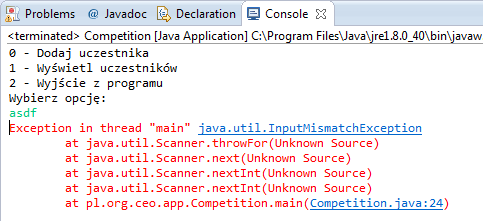
\includegraphics{inputmismatch.png}\hfill}

Aplikacja w tej sytuacji przestaje działać, a dane zostają utracone. W Javie istnieje jednak dosyć prosty mechanizm obsługi sytuacji wyjątkowych za pomocą bloku try catch. Jego ogólna konstrukcja wygląda następująco:

\begin{Verbatim}[commandchars=\\\{\}]
try \PYGZob{}
  //instrukcje mogące wygenerować wyjątek
\PYGZcb{} catch(typ\PYGZus{}wyjatku nazwa\PYGZus{}zmiennej) \PYGZob{}
  //instrukcje, które zostaną wykonane po wygenerowaniu wyjątku
\PYGZcb{} finally \PYGZob{}
  //instrukcje, które wykonają się zawsze, niezależnie, czy wyjątek wystąpi, czy też nie (blok opcjonalny)
\PYGZcb{}
\end{Verbatim}

W naszym kodzie w bloku try można oczywiście umieścić odczyt danych, czyli wywołanie metody \emph{nextInt()}. Można także w nim umieścić dużo większy fragment kodu, jednak warto się zastanowić, czy na pewno się to opłaca i czy pomoże nam to w identyfikacji konkretnego problemu.

\emph{plik Competition.java}

\begin{Verbatim}[commandchars=\\\{\},numbers=left,firstnumber=1,stepnumber=1]
\PYG{k+kd}{public} \PYG{k+kd}{class} \PYG{n+nc}{Competition} \PYG{o}{\PYGZob{}}

    \PYG{c+c1}{//reszta kodu bez zmian}

    \PYG{k+kd}{public} \PYG{k+kd}{static} \PYG{k+kt}{void} \PYG{n+nf}{main}\PYG{o}{(}\PYG{n}{String}\PYG{o}{[}\PYG{o}{]} \PYG{n}{args}\PYG{o}{)} \PYG{o}{\PYGZob{}}
        \PYG{n}{competitors} \PYG{o}{=} \PYG{k}{new} \PYG{n}{Person}\PYG{o}{[}\PYG{l+m+mi}{100}\PYG{o}{]}\PYG{o}{;}
        \PYG{n}{competitorsNumber} \PYG{o}{=} \PYG{l+m+mi}{0}\PYG{o}{;}
        \PYG{n}{Scanner} \PYG{n}{sc} \PYG{o}{=} \PYG{k}{new} \PYG{n}{Scanner}\PYG{o}{(}\PYG{n}{System}\PYG{o}{.}\PYG{n+na}{in}\PYG{o}{)}\PYG{o}{;}
        \PYG{k+kt}{int} \PYG{n}{option} \PYG{o}{=} \PYG{l+m+mi}{0}\PYG{o}{;}

        \PYG{k}{do} \PYG{o}{\PYGZob{}}
            \PYG{n}{printOptions}\PYG{o}{(}\PYG{o}{)}\PYG{o}{;}
            \PYG{k}{try} \PYG{o}{\PYGZob{}}
                \PYG{n}{option} \PYG{o}{=} \PYG{n}{sc}\PYG{o}{.}\PYG{n+na}{nextInt}\PYG{o}{(}\PYG{o}{)}\PYG{o}{;}
                \PYG{n}{sc}\PYG{o}{.}\PYG{n+na}{nextLine}\PYG{o}{(}\PYG{o}{)}\PYG{o}{;}
            \PYG{o}{\PYGZcb{}} \PYG{k}{catch}\PYG{o}{(}\PYG{n}{InputMismatchException} \PYG{n}{exc}\PYG{o}{)} \PYG{o}{\PYGZob{}}
                \PYG{n}{sc}\PYG{o}{.}\PYG{n+na}{nextLine}\PYG{o}{(}\PYG{o}{)}\PYG{o}{;} \PYG{c+c1}{//\PYGZdq{}zjadamy\PYGZdq{} znak nowej linii z bufora}
                \PYG{n}{System}\PYG{o}{.}\PYG{n+na}{out}\PYG{o}{.}\PYG{n+na}{println}\PYG{o}{(}\PYG{l+s}{\PYGZdq{}\PYGZhy{}\PYGZhy{}\PYGZhy{}\PYGZhy{}\PYGZhy{}\PYGZhy{}\PYGZhy{}\PYGZhy{}\PYGZhy{}\PYGZhy{}\PYGZhy{}\PYGZhy{}\PYGZhy{}\PYGZhy{}\PYGZhy{}\PYGZhy{}\PYGZhy{}\PYGZhy{}\PYGZhy{}\PYGZhy{}\PYGZdq{}}\PYG{o}{)}\PYG{o}{;}
                \PYG{n}{System}\PYG{o}{.}\PYG{n+na}{out}\PYG{o}{.}\PYG{n+na}{println}\PYG{o}{(}\PYG{l+s}{\PYGZdq{}Dane w nieprawidłowym formacie \PYGZdq{}}\PYG{o}{)}\PYG{o}{;}
                \PYG{k}{continue}\PYG{o}{;} \PYG{c+c1}{//przejście do kolejnej iteracji pętli}
            \PYG{o}{\PYGZcb{}}

            \PYG{k}{switch} \PYG{o}{(}\PYG{n}{option}\PYG{o}{)} \PYG{o}{\PYGZob{}}
            \PYG{k}{case} \PYG{n+nl}{ADD\PYGZus{}COMPETITOR:}
                \PYG{n}{addCompetitor}\PYG{o}{(}\PYG{n}{sc}\PYG{o}{)}\PYG{o}{;}
                \PYG{k}{break}\PYG{o}{;}
            \PYG{k}{case} \PYG{n+nl}{PRINT\PYGZus{}ALL:}
                \PYG{n}{printCompetitors}\PYG{o}{(}\PYG{o}{)}\PYG{o}{;}
                \PYG{k}{break}\PYG{o}{;}
            \PYG{k}{case} \PYG{n+nl}{EXIT:}
                \PYG{k}{break}\PYG{o}{;}
            \PYG{o}{\PYGZcb{}}
        \PYG{o}{\PYGZcb{}} \PYG{k}{while} \PYG{o}{(}\PYG{n}{option} \PYG{o}{!}\PYG{o}{=} \PYG{n}{EXIT}\PYG{o}{)}\PYG{o}{;}

    \PYG{o}{\PYGZcb{}}

    \PYG{c+c1}{//reszta kodu bez zmian}
\PYG{o}{\PYGZcb{}}
\end{Verbatim}

Jeżeli użytkownik wprowadzi teraz niepoprawne dane podczas przypisania \emph{option = sc.nextInt();} wygenerowany zostanie wyjątek, który jednak obsługujemy w bloku try-catch, a tym samym możemy zapobiec zakońćzeniu programu. Ponieważ po wygenerowaniu wyjątku sterowanie programu jest przekazywane natychmiast do bloku catch, musimy w pierwszej kolejności pozbyć się z bufora znaku nowej linii, który pozostaje po wywołaniu metody nextInt(). Następnie wyświetlamy komunikat o błędzie i przechodzimy do kolejnej iteracji pętli dzięki instrukcji continue. Będzie się tak działo za każdym razem, gdy użytkownik wprowadzi wartość niezgodną z typem int.

Blok finally jest w tym przypadku zbędny. Przydatny będzie natomiast, gdy będziemy chcieli zamknąć strumień, czy plik niezależnie od tego, czy błąd wystąpił, czy nie.


\subsection{Wyjątki - deklaracja throws}
\label{wyjkol:wyjatki-deklaracja-throws}
Istnieją takie sytuacje, w których nie chcemy obsługiwać wyjątków za pomocą bloku try-catch, bo zwyczajnie nie będziemy w stanie nic z tym problemem zrobić. W takiej sytuacji możemy przekazać wyjątek wyżej i dać osobie korzystającej z naszego kodu możliwość zadecydowania, czy chce obsłużyć dany wyjątek, czy też również nic z nim nie robić. Przykładem takiego działania jest metoda \emph{nextInt()} klasy Scanner - może ona generować trzy różne wyjątki, które możemy obsłużyć tak jak w powyższym kodzie, albo je pominąć, tak jak robiliśmy to wcześniej.

\emph{plik Competition.java}

\begin{Verbatim}[commandchars=\\\{\},numbers=left,firstnumber=1,stepnumber=1]
\PYG{k+kn}{package} \PYG{n}{pl}\PYG{o}{.}\PYG{n+na}{org}\PYG{o}{.}\PYG{n+na}{ceo}\PYG{o}{.}\PYG{n+na}{app}\PYG{o}{;}

\PYG{k+kn}{import} \PYG{n+nn}{java.util.InputMismatchException}\PYG{o}{;}
\PYG{k+kn}{import} \PYG{n+nn}{java.util.Scanner}\PYG{o}{;}

\PYG{k+kn}{import} \PYG{n+nn}{pl.org.ceo.data.Person}\PYG{o}{;}

\PYG{k+kd}{public} \PYG{k+kd}{class} \PYG{n+nc}{Competition} \PYG{o}{\PYGZob{}}

    \PYG{k+kd}{public} \PYG{k+kd}{static} \PYG{k+kd}{final} \PYG{k+kt}{int} \PYG{n}{ADD\PYGZus{}COMPETITOR} \PYG{o}{=} \PYG{l+m+mi}{0}\PYG{o}{;}
    \PYG{k+kd}{public} \PYG{k+kd}{static} \PYG{k+kd}{final} \PYG{k+kt}{int} \PYG{n}{PRINT\PYGZus{}ALL} \PYG{o}{=} \PYG{l+m+mi}{1}\PYG{o}{;}
    \PYG{k+kd}{public} \PYG{k+kd}{static} \PYG{k+kd}{final} \PYG{k+kt}{int} \PYG{n}{EXIT} \PYG{o}{=} \PYG{l+m+mi}{2}\PYG{o}{;}

    \PYG{k+kd}{private} \PYG{k+kd}{static} \PYG{n}{Person}\PYG{o}{[}\PYG{o}{]} \PYG{n}{competitors}\PYG{o}{;}
    \PYG{k+kd}{private} \PYG{k+kd}{static} \PYG{k+kt}{int} \PYG{n}{competitorsNumber}\PYG{o}{;}

    \PYG{k+kd}{public} \PYG{k+kd}{static} \PYG{k+kt}{void} \PYG{n+nf}{main}\PYG{o}{(}\PYG{n}{String}\PYG{o}{[}\PYG{o}{]} \PYG{n}{args}\PYG{o}{)} \PYG{o}{\PYGZob{}}
        \PYG{n}{competitors} \PYG{o}{=} \PYG{k}{new} \PYG{n}{Person}\PYG{o}{[}\PYG{l+m+mi}{1}\PYG{o}{]}\PYG{o}{;}
        \PYG{n}{competitorsNumber} \PYG{o}{=} \PYG{l+m+mi}{0}\PYG{o}{;}
        \PYG{n}{Scanner} \PYG{n}{sc} \PYG{o}{=} \PYG{k}{new} \PYG{n}{Scanner}\PYG{o}{(}\PYG{n}{System}\PYG{o}{.}\PYG{n+na}{in}\PYG{o}{)}\PYG{o}{;}
        \PYG{k+kt}{int} \PYG{n}{option} \PYG{o}{=} \PYG{l+m+mi}{0}\PYG{o}{;}

        \PYG{k}{do} \PYG{o}{\PYGZob{}}
            \PYG{n}{printOptions}\PYG{o}{(}\PYG{o}{)}\PYG{o}{;}
            \PYG{k}{try} \PYG{o}{\PYGZob{}}
                \PYG{n}{option} \PYG{o}{=} \PYG{n}{sc}\PYG{o}{.}\PYG{n+na}{nextInt}\PYG{o}{(}\PYG{o}{)}\PYG{o}{;}
                \PYG{n}{sc}\PYG{o}{.}\PYG{n+na}{nextLine}\PYG{o}{(}\PYG{o}{)}\PYG{o}{;}
            \PYG{o}{\PYGZcb{}} \PYG{k}{catch}\PYG{o}{(}\PYG{n}{InputMismatchException} \PYG{n}{exc}\PYG{o}{)} \PYG{o}{\PYGZob{}}
                \PYG{n}{sc}\PYG{o}{.}\PYG{n+na}{nextLine}\PYG{o}{(}\PYG{o}{)}\PYG{o}{;}
                \PYG{n}{System}\PYG{o}{.}\PYG{n+na}{out}\PYG{o}{.}\PYG{n+na}{println}\PYG{o}{(}\PYG{l+s}{\PYGZdq{}\PYGZhy{}\PYGZhy{}\PYGZhy{}\PYGZhy{}\PYGZhy{}\PYGZhy{}\PYGZhy{}\PYGZhy{}\PYGZhy{}\PYGZhy{}\PYGZhy{}\PYGZhy{}\PYGZhy{}\PYGZhy{}\PYGZhy{}\PYGZhy{}\PYGZhy{}\PYGZhy{}\PYGZhy{}\PYGZhy{}\PYGZdq{}}\PYG{o}{)}\PYG{o}{;}
                \PYG{n}{System}\PYG{o}{.}\PYG{n+na}{out}\PYG{o}{.}\PYG{n+na}{println}\PYG{o}{(}\PYG{l+s}{\PYGZdq{}Dane w nieprawidłowym formacie \PYGZdq{}}\PYG{o}{)}\PYG{o}{;}
                \PYG{k}{continue}\PYG{o}{;}
            \PYG{o}{\PYGZcb{}}

            \PYG{k}{switch} \PYG{o}{(}\PYG{n}{option}\PYG{o}{)} \PYG{o}{\PYGZob{}}
            \PYG{k}{case} \PYG{n+nl}{ADD\PYGZus{}COMPETITOR:}
                \PYG{k}{try} \PYG{o}{\PYGZob{}}
                    \PYG{n}{addCompetitor}\PYG{o}{(}\PYG{n}{sc}\PYG{o}{)}\PYG{o}{;}
                \PYG{o}{\PYGZcb{}} \PYG{k}{catch}\PYG{o}{(}\PYG{n}{InputMismatchException} \PYG{n}{e}\PYG{o}{)} \PYG{o}{\PYGZob{}}
                    \PYG{n}{sc}\PYG{o}{.}\PYG{n+na}{nextLine}\PYG{o}{(}\PYG{o}{)}\PYG{o}{;}
                    \PYG{n}{System}\PYG{o}{.}\PYG{n+na}{out}\PYG{o}{.}\PYG{n+na}{println}\PYG{o}{(}\PYG{l+s}{\PYGZdq{}\PYGZhy{}\PYGZhy{}\PYGZhy{}\PYGZhy{}\PYGZhy{}\PYGZhy{}\PYGZhy{}\PYGZhy{}\PYGZhy{}\PYGZhy{}\PYGZhy{}\PYGZhy{}\PYGZhy{}\PYGZhy{}\PYGZhy{}\PYGZhy{}\PYGZhy{}\PYGZhy{}\PYGZhy{}\PYGZhy{}\PYGZdq{}}\PYG{o}{)}\PYG{o}{;}
                    \PYG{n}{System}\PYG{o}{.}\PYG{n+na}{out}\PYG{o}{.}\PYG{n+na}{println}\PYG{o}{(}\PYG{l+s}{\PYGZdq{}Błąd odczytu danych\PYGZdq{}}\PYG{o}{)}\PYG{o}{;}
                \PYG{o}{\PYGZcb{}} \PYG{k}{catch} \PYG{o}{(}\PYG{n}{ArrayIndexOutOfBoundsException} \PYG{n}{e}\PYG{o}{)} \PYG{o}{\PYGZob{}}
                    \PYG{n}{System}\PYG{o}{.}\PYG{n+na}{out}\PYG{o}{.}\PYG{n+na}{println}\PYG{o}{(}\PYG{l+s}{\PYGZdq{}\PYGZhy{}\PYGZhy{}\PYGZhy{}\PYGZhy{}\PYGZhy{}\PYGZhy{}\PYGZhy{}\PYGZhy{}\PYGZhy{}\PYGZhy{}\PYGZhy{}\PYGZhy{}\PYGZhy{}\PYGZhy{}\PYGZhy{}\PYGZhy{}\PYGZhy{}\PYGZhy{}\PYGZhy{}\PYGZhy{}\PYGZdq{}}\PYG{o}{)}\PYG{o}{;}
                    \PYG{n}{System}\PYG{o}{.}\PYG{n+na}{out}\PYG{o}{.}\PYG{n+na}{println}\PYG{o}{(}\PYG{n}{e}\PYG{o}{.}\PYG{n+na}{getMessage}\PYG{o}{(}\PYG{o}{)}\PYG{o}{)}\PYG{o}{;}
                \PYG{o}{\PYGZcb{}}
                \PYG{k}{break}\PYG{o}{;}
            \PYG{k}{case} \PYG{n+nl}{PRINT\PYGZus{}ALL:}
                \PYG{n}{printCompetitors}\PYG{o}{(}\PYG{o}{)}\PYG{o}{;}
                \PYG{k}{break}\PYG{o}{;}
            \PYG{k}{case} \PYG{n+nl}{EXIT:}
                \PYG{k}{break}\PYG{o}{;}
            \PYG{o}{\PYGZcb{}}
        \PYG{o}{\PYGZcb{}} \PYG{k}{while} \PYG{o}{(}\PYG{n}{option} \PYG{o}{!}\PYG{o}{=} \PYG{n}{EXIT}\PYG{o}{)}\PYG{o}{;}

        \PYG{n}{sc}\PYG{o}{.}\PYG{n+na}{close}\PYG{o}{(}\PYG{o}{)}\PYG{o}{;}

    \PYG{o}{\PYGZcb{}}

    \PYG{k+kd}{private} \PYG{k+kd}{static} \PYG{k+kt}{void} \PYG{n+nf}{printCompetitors}\PYG{o}{(}\PYG{o}{)} \PYG{o}{\PYGZob{}}
        \PYG{n}{System}\PYG{o}{.}\PYG{n+na}{out}\PYG{o}{.}\PYG{n+na}{println}\PYG{o}{(}\PYG{l+s}{\PYGZdq{}\PYGZhy{}\PYGZhy{}\PYGZhy{}\PYGZhy{}\PYGZhy{}\PYGZhy{}\PYGZhy{}\PYGZhy{}\PYGZhy{}\PYGZhy{}\PYGZhy{}\PYGZhy{}\PYGZhy{}\PYGZhy{}\PYGZhy{}\PYGZhy{}\PYGZhy{}\PYGZhy{}\PYGZhy{}\PYGZhy{}\PYGZdq{}}\PYG{o}{)}\PYG{o}{;}
        \PYG{n}{System}\PYG{o}{.}\PYG{n+na}{out}\PYG{o}{.}\PYG{n+na}{println}\PYG{o}{(}\PYG{l+s}{\PYGZdq{}Lista uczestników:\PYGZdq{}}\PYG{o}{)}\PYG{o}{;}
        \PYG{k}{for}\PYG{o}{(}\PYG{k+kt}{int} \PYG{n}{i}\PYG{o}{=}\PYG{l+m+mi}{0}\PYG{o}{;} \PYG{n}{i} \PYG{o}{\PYGZlt{}} \PYG{n}{competitorsNumber}\PYG{o}{;} \PYG{n}{i}\PYG{o}{+}\PYG{o}{+}\PYG{o}{)} \PYG{o}{\PYGZob{}}
            \PYG{n}{System}\PYG{o}{.}\PYG{n+na}{out}\PYG{o}{.}\PYG{n+na}{println}\PYG{o}{(}\PYG{n}{competitors}\PYG{o}{[}\PYG{n}{i}\PYG{o}{]}\PYG{o}{.}\PYG{n+na}{toString}\PYG{o}{(}\PYG{o}{)}\PYG{o}{)}\PYG{o}{;}
        \PYG{o}{\PYGZcb{}}
    \PYG{o}{\PYGZcb{}}

    \PYG{k+kd}{private} \PYG{k+kd}{static} \PYG{k+kt}{void} \PYG{n+nf}{addCompetitor}\PYG{o}{(}\PYG{n}{Scanner} \PYG{n}{sc}\PYG{o}{)} \PYG{k+kd}{throws} \PYG{n}{InputMismatchException}\PYG{o}{,} \PYG{n}{ArrayIndexOutOfBoundsException} \PYG{o}{\PYGZob{}}
        \PYG{k}{if}\PYG{o}{(}\PYG{n}{competitorsNumber} \PYG{o}{\PYGZlt{}} \PYG{n}{competitors}\PYG{o}{.}\PYG{n+na}{length}\PYG{o}{)} \PYG{o}{\PYGZob{}}
            \PYG{n}{Person} \PYG{n}{person} \PYG{o}{=} \PYG{k}{new} \PYG{n}{Person}\PYG{o}{(}\PYG{o}{)}\PYG{o}{;}
            \PYG{n}{System}\PYG{o}{.}\PYG{n+na}{out}\PYG{o}{.}\PYG{n+na}{println}\PYG{o}{(}\PYG{l+s}{\PYGZdq{}\PYGZhy{}\PYGZhy{}\PYGZhy{}\PYGZhy{}\PYGZhy{}\PYGZhy{}\PYGZhy{}\PYGZhy{}\PYGZhy{}\PYGZhy{}\PYGZhy{}\PYGZhy{}\PYGZhy{}\PYGZhy{}\PYGZhy{}\PYGZhy{}\PYGZhy{}\PYGZhy{}\PYGZhy{}\PYGZhy{}\PYGZdq{}}\PYG{o}{)}\PYG{o}{;}
            \PYG{n}{System}\PYG{o}{.}\PYG{n+na}{out}\PYG{o}{.}\PYG{n+na}{println}\PYG{o}{(}\PYG{l+s}{\PYGZdq{}Dodawanie nowego uczestnika: \PYGZdq{}}\PYG{o}{)}\PYG{o}{;}
            \PYG{n}{System}\PYG{o}{.}\PYG{n+na}{out}\PYG{o}{.}\PYG{n+na}{println}\PYG{o}{(}\PYG{l+s}{\PYGZdq{}Imię: \PYGZdq{}}\PYG{o}{)}\PYG{o}{;}
            \PYG{n}{person}\PYG{o}{.}\PYG{n+na}{setFirstName}\PYG{o}{(}\PYG{n}{sc}\PYG{o}{.}\PYG{n+na}{nextLine}\PYG{o}{(}\PYG{o}{)}\PYG{o}{)}\PYG{o}{;}
            \PYG{n}{System}\PYG{o}{.}\PYG{n+na}{out}\PYG{o}{.}\PYG{n+na}{println}\PYG{o}{(}\PYG{l+s}{\PYGZdq{}Nazwisko\PYGZdq{}}\PYG{o}{)}\PYG{o}{;}
            \PYG{n}{person}\PYG{o}{.}\PYG{n+na}{setLastName}\PYG{o}{(}\PYG{n}{sc}\PYG{o}{.}\PYG{n+na}{nextLine}\PYG{o}{(}\PYG{o}{)}\PYG{o}{)}\PYG{o}{;}
            \PYG{n}{System}\PYG{o}{.}\PYG{n+na}{out}\PYG{o}{.}\PYG{n+na}{println}\PYG{o}{(}\PYG{l+s}{\PYGZdq{}PESEL:\PYGZdq{}}\PYG{o}{)}\PYG{o}{;}
            \PYG{n}{person}\PYG{o}{.}\PYG{n+na}{setPesel}\PYG{o}{(}\PYG{n}{sc}\PYG{o}{.}\PYG{n+na}{nextLine}\PYG{o}{(}\PYG{o}{)}\PYG{o}{)}\PYG{o}{;}
            \PYG{n}{System}\PYG{o}{.}\PYG{n+na}{out}\PYG{o}{.}\PYG{n+na}{println}\PYG{o}{(}\PYG{l+s}{\PYGZdq{}Wiek:\PYGZdq{}}\PYG{o}{)}\PYG{o}{;}
            \PYG{n}{person}\PYG{o}{.}\PYG{n+na}{setAge}\PYG{o}{(}\PYG{n}{sc}\PYG{o}{.}\PYG{n+na}{nextInt}\PYG{o}{(}\PYG{o}{)}\PYG{o}{)}\PYG{o}{;}
            \PYG{n}{sc}\PYG{o}{.}\PYG{n+na}{nextLine}\PYG{o}{(}\PYG{o}{)}\PYG{o}{;}

            \PYG{n}{competitors}\PYG{o}{[}\PYG{n}{competitorsNumber}\PYG{o}{]} \PYG{o}{=} \PYG{n}{person}\PYG{o}{;}
            \PYG{n}{competitorsNumber}\PYG{o}{+}\PYG{o}{+}\PYG{o}{;}
        \PYG{o}{\PYGZcb{}} \PYG{k}{else} \PYG{o}{\PYGZob{}}
            \PYG{c+c1}{//jeżeli tablica jest pełna, tworzymy wyjątek, który o tym informuje}
            \PYG{k}{throw} \PYG{k}{new} \PYG{n+nf}{ArrayIndexOutOfBoundsException}\PYG{o}{(}\PYG{l+s}{\PYGZdq{}Osiągnięto maksymalną liczbę uczestników\PYGZdq{}}\PYG{o}{)}\PYG{o}{;}
        \PYG{o}{\PYGZcb{}}
    \PYG{o}{\PYGZcb{}}

    \PYG{k+kd}{private} \PYG{k+kd}{static} \PYG{k+kt}{void} \PYG{n+nf}{printOptions}\PYG{o}{(}\PYG{o}{)} \PYG{o}{\PYGZob{}}
        \PYG{n}{System}\PYG{o}{.}\PYG{n+na}{out}\PYG{o}{.}\PYG{n+na}{println}\PYG{o}{(}\PYG{l+s}{\PYGZdq{}\PYGZhy{}\PYGZhy{}\PYGZhy{}\PYGZhy{}\PYGZhy{}\PYGZhy{}\PYGZhy{}\PYGZhy{}\PYGZhy{}\PYGZhy{}\PYGZhy{}\PYGZhy{}\PYGZhy{}\PYGZhy{}\PYGZhy{}\PYGZhy{}\PYGZhy{}\PYGZhy{}\PYGZhy{}\PYGZhy{}\PYGZdq{}}\PYG{o}{)}\PYG{o}{;}
        \PYG{n}{System}\PYG{o}{.}\PYG{n+na}{out}\PYG{o}{.}\PYG{n+na}{println}\PYG{o}{(}\PYG{l+s}{\PYGZdq{}Dostępne opcje: \PYGZdq{}}\PYG{o}{)}\PYG{o}{;}
        \PYG{n}{System}\PYG{o}{.}\PYG{n+na}{out}\PYG{o}{.}\PYG{n+na}{println}\PYG{o}{(}\PYG{n}{ADD\PYGZus{}COMPETITOR} \PYG{o}{+} \PYG{l+s}{\PYGZdq{} \PYGZhy{} Dodaj uczestnika\PYGZdq{}}\PYG{o}{)}\PYG{o}{;}
        \PYG{n}{System}\PYG{o}{.}\PYG{n+na}{out}\PYG{o}{.}\PYG{n+na}{println}\PYG{o}{(}\PYG{n}{PRINT\PYGZus{}ALL} \PYG{o}{+} \PYG{l+s}{\PYGZdq{} \PYGZhy{} Wyświetl uczestników\PYGZdq{}}\PYG{o}{)}\PYG{o}{;}
        \PYG{n}{System}\PYG{o}{.}\PYG{n+na}{out}\PYG{o}{.}\PYG{n+na}{println}\PYG{o}{(}\PYG{n}{EXIT} \PYG{o}{+} \PYG{l+s}{\PYGZdq{} \PYGZhy{} Wyjście z programu\PYGZdq{}}\PYG{o}{)}\PYG{o}{;}
        \PYG{n}{System}\PYG{o}{.}\PYG{n+na}{out}\PYG{o}{.}\PYG{n+na}{println}\PYG{o}{(}\PYG{l+s}{\PYGZdq{}Wybierz opcję: \PYGZdq{}}\PYG{o}{)}\PYG{o}{;}
    \PYG{o}{\PYGZcb{}}
\PYG{o}{\PYGZcb{}}
\end{Verbatim}

W naszym programie sensownym miejscem, w którym możemy stworzyć i rzucić wyjątek jest metoda \emph{addCompetitor()}. Jeżeli tablica, którą utworzyliśmy będzie już pełna, wygenerujemy wyjątek, który pojawia się, gdy próbujemy odwoływać się do indeksu tablicy wykraczającego poza zakres, czyli \emph{ArrayIndexOutOfBoundsException}. W kodzie używamy także metody \emph{getInt()} klasy Scanner, jednak tym razem nie obsługujemy tu wyjątku, a jedynie dodajemy o nim informację w sygnaturze metody (lepiej jest go obsłużyć, ale na potrzeby ćwiczenia zróbmy to w ten sposób).

Oba wyjątki, czyli ArrayIndexOutOfBoundsException i InputMismatchException nie muszą być obsługiwane, więc informacja w sygnaturze metody jest bardziej komunikatem dla programisty, czego może się spodziewać. Oba wyjątki obsługujemy w osobnych blokach catch już bezpośrednio w bloku konstrukcji switch umieszczonej w metodzie \emph{main()}. Jak widzisz do jednego bloku try możemy podpiąć kilka bloków catch do obsługi różnych wyjątków - działa to podobnie do instrukcji warunkowej if else.

Rozmiar tablicy w powyższym przykładzie zmieniliśmy na 1, abyś mógł przetestować działanie wyjątku. Przy próbie dodania drugiego uczestnika do tablicy, generujemy wyjątek ArrayIndexOutOfBoundsException, z którego następnie już w bloku catch() pobieramy informację przekazaną w konstruktorze za pomocą metody \emph{e.getMessage()}.

{\hfill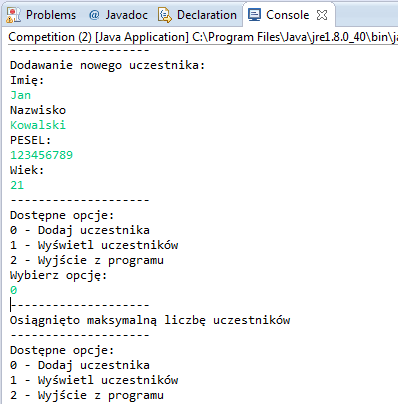
\includegraphics{aioobe.png}\hfill}


\subsection{Kolekcje}
\label{wyjkol:kolekcje}
Mówiąc o kolekcjach w Javie będziemy mieli na myśli Collections framework, czyli specjalny zestaw interfejsów i klas, które są przeznaczone do przechowywania różnych kolekcji obiektów. Hierarchię kolekcji w języku Java przedstawiono na poniższym diagramie, my omówimy najczęściej wykorzystywane listy.

Zbiory, listy i kolejki:

{\hfill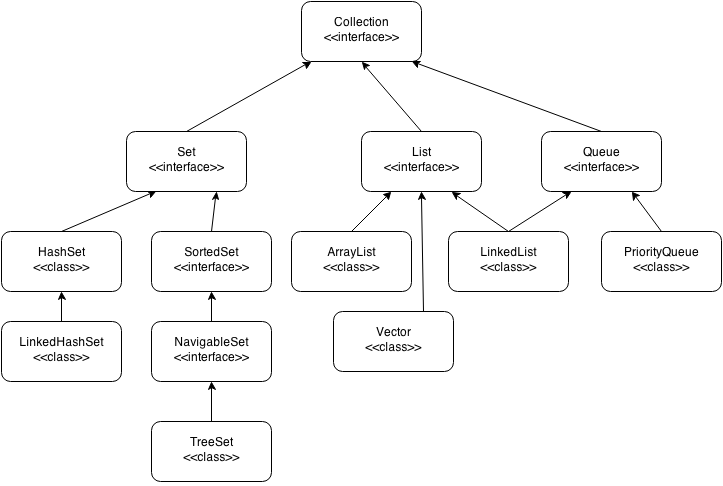
\includegraphics{collections.png}\hfill}

oraz mapy:

{\hfill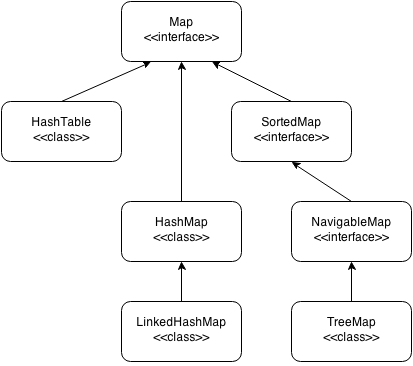
\includegraphics{maps_collections.png}\hfill}


\subsection{Typy opakowujące}
\label{wyjkol:typy-opakowujace}
Pierwszą rzeczą, którą musimy wyjaśnić przed przejściem do omówienia list oraz zbiorów są typy opakowujące typów prostych. Jest to spowodowane tym, że jak wspomnieliśmy na wstępie, kolekcje służą do przechowywania obiektów, a typy proste takie jak int, czy double typami obiektowymi nie są. Typem obiektowym jest natomiast String, w którego przypadku nie napotkamy na większe problemy.

Każdy z typów prostych ma swój odpowiednik obiektowy. Lista klas reprezentujących poszczególne z nich przedstawia się następująco:
\begin{itemize}
\item {} 
byte - Byte

\item {} 
short - Short

\item {} 
int - Integer

\item {} 
long - Long

\item {} 
float - Float

\item {} 
double - Double

\item {} 
boolean - Boolean

\item {} 
char - Character

\end{itemize}

Jak widzisz w większości przypadków zmianie ulega jedynie litera z małej na wielką. W celu zamiany wartości typu prostego, np. liczby 15, na obiekt typu Integer reprezentujący wartość 15 należy wykorzystać statyczną metodę \emph{valueOf()}, którą posiada każdy z wyżej wymieninych typów. Metoda ta jest dostępna w kilku przeciążonych wersjach, więc jako jej argument możemy podać zarówno liczbę w formie typu prostego lub jako String. Innym sposobem jest po prostu skorzystanie z konstruktora danej klasy - oba podejścia działają w praktyce tak samo.

\emph{plik Wrappers.java}

\begin{Verbatim}[commandchars=\\\{\},numbers=left,firstnumber=1,stepnumber=1]
\PYG{k+kd}{public} \PYG{k+kd}{class} \PYG{n+nc}{Wrappers} \PYG{o}{\PYGZob{}}
    \PYG{k+kd}{public} \PYG{k+kd}{static} \PYG{k+kt}{void} \PYG{n+nf}{main}\PYG{o}{(}\PYG{n}{String}\PYG{o}{[}\PYG{o}{]} \PYG{n}{args}\PYG{o}{)} \PYG{o}{\PYGZob{}}
        \PYG{c+c1}{//konstruktor na podstawie liczby}
        \PYG{n}{Integer} \PYG{n}{num1} \PYG{o}{=} \PYG{k}{new} \PYG{n}{Integer}\PYG{o}{(}\PYG{l+m+mi}{15}\PYG{o}{)}\PYG{o}{;}
        \PYG{c+c1}{//konstruktor na podstawie Stringa}
        \PYG{n}{Integer} \PYG{n}{num2} \PYG{o}{=} \PYG{k}{new} \PYG{n}{Integer}\PYG{o}{(}\PYG{l+s}{\PYGZdq{}15\PYGZdq{}}\PYG{o}{)}\PYG{o}{;}

        \PYG{c+c1}{//metody valueOf()}
        \PYG{n}{Integer} \PYG{n}{num3} \PYG{o}{=} \PYG{n}{Integer}\PYG{o}{.}\PYG{n+na}{valueOf}\PYG{o}{(}\PYG{l+m+mi}{15}\PYG{o}{)}\PYG{o}{;}
        \PYG{n}{Integer} \PYG{n}{num4} \PYG{o}{=} \PYG{n}{Integer}\PYG{o}{.}\PYG{n+na}{valueOf}\PYG{o}{(}\PYG{l+s}{\PYGZdq{}15\PYGZdq{}}\PYG{o}{)}\PYG{o}{;}

        \PYG{c+c1}{//Porównanie obiektów nie działa tak jak porównywanie typów prostych!}
        \PYG{c+c1}{//do porównywanie obiektów zawsze wykorzystuj metodę equals()}
        \PYG{n}{System}\PYG{o}{.}\PYG{n+na}{out}\PYG{o}{.}\PYG{n+na}{println}\PYG{o}{(}\PYG{l+s}{\PYGZdq{}num1 == num2 = \PYGZdq{}} \PYG{o}{+} \PYG{o}{(}\PYG{n}{num1}\PYG{o}{=}\PYG{o}{=}\PYG{n}{num2}\PYG{o}{)}\PYG{o}{)}\PYG{o}{;}
        \PYG{n}{System}\PYG{o}{.}\PYG{n+na}{out}\PYG{o}{.}\PYG{n+na}{println}\PYG{o}{(}\PYG{l+s}{\PYGZdq{}num1.equals(num2) = \PYGZdq{}} \PYG{o}{+} \PYG{o}{(}\PYG{n}{num1}\PYG{o}{.}\PYG{n+na}{equals}\PYG{o}{(}\PYG{n}{num2}\PYG{o}{)}\PYG{o}{)}\PYG{o}{)}\PYG{o}{;}
    \PYG{o}{\PYGZcb{}}
\PYG{o}{\PYGZcb{}}
\end{Verbatim}

Ponieważ korzystając z kolekcji byłoby straszną męczarnią konwertowanie typów z prostych na obiektowe i z obiektowych na proste, to w Javie 1.5 wprowadzono mechanizm autoboxingu i unboxingu, czyli automatycznej konwersji pomiędzy typami. Można więc bez problemu przypisać do referencji typu Integer wartość 5, a wirtualna maszyna automatycznie zamieni ją na obiekt.

\emph{plik Autoboxing.java}

\begin{Verbatim}[commandchars=\\\{\},numbers=left,firstnumber=1,stepnumber=1]
\PYG{k+kd}{public} \PYG{k+kd}{class} \PYG{n+nc}{Autoboxing} \PYG{o}{\PYGZob{}}
    \PYG{k+kd}{public} \PYG{k+kd}{static} \PYG{k+kt}{void} \PYG{n+nf}{main}\PYG{o}{(}\PYG{n}{String}\PYG{o}{[}\PYG{o}{]} \PYG{n}{args}\PYG{o}{)} \PYG{o}{\PYGZob{}}
        \PYG{c+c1}{//autoboxing}
        \PYG{n}{Double} \PYG{n}{num1} \PYG{o}{=} \PYG{l+m+mf}{5.54}\PYG{o}{;}
        \PYG{n}{Integer} \PYG{n}{num2} \PYG{o}{=} \PYG{l+m+mi}{200}\PYG{o}{;}

        \PYG{c+c1}{//unboxing}
        \PYG{k+kt}{double} \PYG{n}{num3} \PYG{o}{=} \PYG{n}{num1}\PYG{o}{;}
        \PYG{k+kt}{int} \PYG{n}{num4} \PYG{o}{=} \PYG{n}{num2}\PYG{o}{;}

        \PYG{n}{System}\PYG{o}{.}\PYG{n+na}{out}\PYG{o}{.}\PYG{n+na}{println}\PYG{o}{(}\PYG{l+s}{\PYGZdq{}num1.equals(num2) = \PYGZdq{}} \PYG{o}{+} \PYG{o}{(}\PYG{n}{num1} \PYG{o}{=}\PYG{o}{=} \PYG{n}{num3}\PYG{o}{)}\PYG{o}{)}\PYG{o}{;} \PYG{c+c1}{//true}
    \PYG{o}{\PYGZcb{}}
\PYG{o}{\PYGZcb{}}
\end{Verbatim}

Typ String jest typem obiektowym (dlatego też pisany jest z wielkiej litery), więc nie wymaga dodatkowych zabiegów.


\subsection{Listy}
\label{wyjkol:listy}
Listy to najprostsze struktury danych. Ich głównym zadaniem jest przechowywanie obiektów w uporządkowanej, indeksowanej formie - czyli podobnie jak w przypadku tablic. Istnieją dwa główne typy list:
\begin{itemize}
\item {} 
lista tablicowa (\textbf{ArrayList}) - jej wewnętrzna struktura opiera się dokładnie na tablicy

\item {} 
lista wiązana (\textbf{LinkedList}) - obiekty w niej stanowią skończony ciąg połączonych ze sobą węzłów

\end{itemize}

Na poziomie tego szkolenia nie będziemy zgłębiali różnić pomiędzy tymi strukturami i skupimy się na pierwszej z nich, jednak warto wiedzieć, że z powodu odmiennej reprezentacji wewnętrznej wydajnosć operacji takich jak usuwanie, czy wyszukiwanie w obu z nich może się znacząco różnić w przypadku dużych grup danych.

Listę tworzymy w następujący sposób:

\begin{Verbatim}[commandchars=\\\{\}]
ArrayList\PYGZlt{}Typ\PYGZus{}Danych\PYGZgt{} nazwaListy = new ArrayList\PYGZlt{}\PYGZgt{}();
//np.
ArrayList\PYGZlt{}String\PYGZgt{} names = new ArrayList\PYGZlt{}\PYGZgt{}();
\end{Verbatim}

Ponieważ typy kolekcyjne stanowią jednak pewną hierarchię dziedziczenia, warto również korzystać z zalet polimorfizmu i stosować ogólniejszy typ referencji, do którego można przypisać zarówno LinkedListę jak i ArrayListę.

\begin{Verbatim}[commandchars=\\\{\}]
List\PYGZlt{}String\PYGZgt{} names = new ArrayList\PYGZlt{}\PYGZgt{}();
\end{Verbatim}

Mamy jednak wtedy dostęp jedynie do metod z typu referencji, czyli interfejsu List (chyba, że zastosujemy rzutowanie na typ ArrayList).
Pomiędzy ostrymi nawiasami określamy typ danych jaki będzie przechowywała dana lista. Powiemy dzięki temu, że kolekcja jest \textbf{typem generycznym}.

Na listach możemy wykonywać podstawowe operacje takie jak:
\begin{itemize}
\item {} 
dodawanie - metoda \textbf{add(Object obiekt)}

\item {} 
usuwanie - metoda \textbf{remove(int index)} jeśli chcemy usunąć element o wskazanym indeksie lub \textbf{remove(Object o)} jeżeli chcemy usunąć obiekt, dla którego porównanie za pomocą metody equals() z przekazanym parametrem zwróci true

\item {} 
pobranie elementu z listy - metoda \textbf{get()} - analogicznie jak w przypadku tablic listy indeksowane są od 0

\item {} 
sprawdzenie rozmiaru listy - metoda \textbf{size()}

\item {} 
sprawdzenie, czy dany obiekt znajduje się w liście - metoda \textbf{contains(Object obiekt)}

\end{itemize}

\emph{plik Collect.java}

\begin{Verbatim}[commandchars=\\\{\},numbers=left,firstnumber=1,stepnumber=1]
\PYG{k+kn}{package} \PYG{n}{pl}\PYG{o}{.}\PYG{n+na}{org}\PYG{o}{.}\PYG{n+na}{ceo}\PYG{o}{.}\PYG{n+na}{main}\PYG{o}{;}

\PYG{k+kn}{import} \PYG{n+nn}{java.util.ArrayList}\PYG{o}{;}
\PYG{k+kn}{import} \PYG{n+nn}{java.util.List}\PYG{o}{;}

\PYG{k+kd}{public} \PYG{k+kd}{class} \PYG{n+nc}{Collect} \PYG{o}{\PYGZob{}}
    \PYG{k+kd}{public} \PYG{k+kd}{static} \PYG{k+kt}{void} \PYG{n+nf}{main}\PYG{o}{(}\PYG{n}{String}\PYG{o}{[}\PYG{o}{]} \PYG{n}{args}\PYG{o}{)} \PYG{o}{\PYGZob{}}
        \PYG{n}{List}\PYG{o}{\PYGZlt{}}\PYG{n}{String}\PYG{o}{\PYGZgt{}} \PYG{n}{names} \PYG{o}{=} \PYG{k}{new} \PYG{n}{ArrayList}\PYG{o}{\PYGZlt{}}\PYG{o}{\PYGZgt{}}\PYG{o}{(}\PYG{o}{)}\PYG{o}{;}

        \PYG{n}{names}\PYG{o}{.}\PYG{n+na}{add}\PYG{o}{(}\PYG{l+s}{\PYGZdq{}Jan\PYGZdq{}}\PYG{o}{)}\PYG{o}{;}
        \PYG{n}{names}\PYG{o}{.}\PYG{n+na}{add}\PYG{o}{(}\PYG{l+s}{\PYGZdq{}Wojtek\PYGZdq{}}\PYG{o}{)}\PYG{o}{;}
        \PYG{n}{names}\PYG{o}{.}\PYG{n+na}{add}\PYG{o}{(}\PYG{l+s}{\PYGZdq{}Kasia\PYGZdq{}}\PYG{o}{)}\PYG{o}{;}

        \PYG{n}{System}\PYG{o}{.}\PYG{n+na}{out}\PYG{o}{.}\PYG{n+na}{println}\PYG{o}{(}\PYG{l+s}{\PYGZdq{}Czy Jan jest na liście: \PYGZdq{}} \PYG{o}{+} \PYG{n}{names}\PYG{o}{.}\PYG{n+na}{contains}\PYG{o}{(}\PYG{l+s}{\PYGZdq{}Jan\PYGZdq{}}\PYG{o}{)}\PYG{o}{)}\PYG{o}{;}
        \PYG{n}{System}\PYG{o}{.}\PYG{n+na}{out}\PYG{o}{.}\PYG{n+na}{println}\PYG{o}{(}\PYG{l+s}{\PYGZdq{}Ile jest osób na liście: \PYGZdq{}} \PYG{o}{+} \PYG{n}{names}\PYG{o}{.}\PYG{n+na}{size}\PYG{o}{(}\PYG{o}{)}\PYG{o}{)}\PYG{o}{;}
        \PYG{n}{System}\PYG{o}{.}\PYG{n+na}{out}\PYG{o}{.}\PYG{n+na}{println}\PYG{o}{(}\PYG{l+s}{\PYGZdq{}A po usunięciu Wojtka \PYGZdq{}}\PYG{o}{)}\PYG{o}{;}
        \PYG{n}{names}\PYG{o}{.}\PYG{n+na}{remove}\PYG{o}{(}\PYG{l+s}{\PYGZdq{}Wojtek\PYGZdq{}}\PYG{o}{)}\PYG{o}{;}
        \PYG{n}{System}\PYG{o}{.}\PYG{n+na}{out}\PYG{o}{.}\PYG{n+na}{println}\PYG{o}{(}\PYG{l+s}{\PYGZdq{}rozmiar to \PYGZdq{}} \PYG{o}{+} \PYG{n}{names}\PYG{o}{.}\PYG{n+na}{size}\PYG{o}{(}\PYG{o}{)}\PYG{o}{)}\PYG{o}{;}
    \PYG{o}{\PYGZcb{}}
\PYG{o}{\PYGZcb{}}
\end{Verbatim}
\begin{description}
\item[{\textbf{Ćwiczenie} \emph{(15 minut)}}] \leavevmode
Przerób program z wcześniejszej części lekcji (zapisy na konkurs) w taki sposób, aby uczestnicy byli dopisywani do listy, a nie tablicy.

\end{description}

\emph{plik Competition.java}

\begin{Verbatim}[commandchars=\\\{\},numbers=left,firstnumber=1,stepnumber=1]
\PYG{k+kn}{package} \PYG{n}{pl}\PYG{o}{.}\PYG{n+na}{org}\PYG{o}{.}\PYG{n+na}{ceo}\PYG{o}{.}\PYG{n+na}{app}\PYG{o}{;}

\PYG{k+kn}{import} \PYG{n+nn}{java.util.ArrayList}\PYG{o}{;}
\PYG{k+kn}{import} \PYG{n+nn}{java.util.InputMismatchException}\PYG{o}{;}
\PYG{k+kn}{import} \PYG{n+nn}{java.util.List}\PYG{o}{;}
\PYG{k+kn}{import} \PYG{n+nn}{java.util.Scanner}\PYG{o}{;}

\PYG{k+kn}{import} \PYG{n+nn}{pl.org.ceo.data.Person}\PYG{o}{;}

\PYG{k+kd}{public} \PYG{k+kd}{class} \PYG{n+nc}{Competition} \PYG{o}{\PYGZob{}}

    \PYG{k+kd}{public} \PYG{k+kd}{static} \PYG{k+kd}{final} \PYG{k+kt}{int} \PYG{n}{ADD\PYGZus{}COMPETITOR} \PYG{o}{=} \PYG{l+m+mi}{0}\PYG{o}{;}
    \PYG{k+kd}{public} \PYG{k+kd}{static} \PYG{k+kd}{final} \PYG{k+kt}{int} \PYG{n}{PRINT\PYGZus{}ALL} \PYG{o}{=} \PYG{l+m+mi}{1}\PYG{o}{;}
    \PYG{k+kd}{public} \PYG{k+kd}{static} \PYG{k+kd}{final} \PYG{k+kt}{int} \PYG{n}{EXIT} \PYG{o}{=} \PYG{l+m+mi}{2}\PYG{o}{;}

    \PYG{c+c1}{// zastępujemy tablicę listą}
    \PYG{k+kd}{private} \PYG{k+kd}{static} \PYG{n}{List}\PYG{o}{\PYGZlt{}}\PYG{n}{Person}\PYG{o}{\PYGZgt{}} \PYG{n}{competitors}\PYG{o}{;}

    \PYG{k+kd}{public} \PYG{k+kd}{static} \PYG{k+kt}{void} \PYG{n+nf}{main}\PYG{o}{(}\PYG{n}{String}\PYG{o}{[}\PYG{o}{]} \PYG{n}{args}\PYG{o}{)} \PYG{o}{\PYGZob{}}
        \PYG{c+c1}{// inicjalizujemy listę}
        \PYG{n}{competitors} \PYG{o}{=} \PYG{k}{new} \PYG{n}{ArrayList}\PYG{o}{\PYGZlt{}}\PYG{o}{\PYGZgt{}}\PYG{o}{(}\PYG{o}{)}\PYG{o}{;}
        \PYG{n}{Scanner} \PYG{n}{sc} \PYG{o}{=} \PYG{k}{new} \PYG{n}{Scanner}\PYG{o}{(}\PYG{n}{System}\PYG{o}{.}\PYG{n+na}{in}\PYG{o}{)}\PYG{o}{;}
        \PYG{k+kt}{int} \PYG{n}{option} \PYG{o}{=} \PYG{l+m+mi}{0}\PYG{o}{;}

        \PYG{k}{do} \PYG{o}{\PYGZob{}}
            \PYG{n}{printOptions}\PYG{o}{(}\PYG{o}{)}\PYG{o}{;}
            \PYG{k}{try} \PYG{o}{\PYGZob{}}
                \PYG{n}{option} \PYG{o}{=} \PYG{n}{sc}\PYG{o}{.}\PYG{n+na}{nextInt}\PYG{o}{(}\PYG{o}{)}\PYG{o}{;}
                \PYG{n}{sc}\PYG{o}{.}\PYG{n+na}{nextLine}\PYG{o}{(}\PYG{o}{)}\PYG{o}{;}
            \PYG{o}{\PYGZcb{}} \PYG{k}{catch} \PYG{o}{(}\PYG{n}{InputMismatchException} \PYG{n}{exc}\PYG{o}{)} \PYG{o}{\PYGZob{}}
                \PYG{n}{sc}\PYG{o}{.}\PYG{n+na}{nextLine}\PYG{o}{(}\PYG{o}{)}\PYG{o}{;}
                \PYG{n}{System}\PYG{o}{.}\PYG{n+na}{out}\PYG{o}{.}\PYG{n+na}{println}\PYG{o}{(}\PYG{l+s}{\PYGZdq{}\PYGZhy{}\PYGZhy{}\PYGZhy{}\PYGZhy{}\PYGZhy{}\PYGZhy{}\PYGZhy{}\PYGZhy{}\PYGZhy{}\PYGZhy{}\PYGZhy{}\PYGZhy{}\PYGZhy{}\PYGZhy{}\PYGZhy{}\PYGZhy{}\PYGZhy{}\PYGZhy{}\PYGZhy{}\PYGZhy{}\PYGZdq{}}\PYG{o}{)}\PYG{o}{;}
                \PYG{n}{System}\PYG{o}{.}\PYG{n+na}{out}\PYG{o}{.}\PYG{n+na}{println}\PYG{o}{(}\PYG{l+s}{\PYGZdq{}Dane w nieprawidłowym formacie \PYGZdq{}}\PYG{o}{)}\PYG{o}{;}
                \PYG{k}{continue}\PYG{o}{;}
            \PYG{o}{\PYGZcb{}}

            \PYG{k}{switch} \PYG{o}{(}\PYG{n}{option}\PYG{o}{)} \PYG{o}{\PYGZob{}}
            \PYG{k}{case} \PYG{n+nl}{ADD\PYGZus{}COMPETITOR:}
                \PYG{k}{try} \PYG{o}{\PYGZob{}}
                    \PYG{n}{addCompetitor}\PYG{o}{(}\PYG{n}{sc}\PYG{o}{)}\PYG{o}{;}
                \PYG{o}{\PYGZcb{}} \PYG{k}{catch} \PYG{o}{(}\PYG{n}{InputMismatchException} \PYG{n}{e}\PYG{o}{)} \PYG{o}{\PYGZob{}}
                    \PYG{n}{sc}\PYG{o}{.}\PYG{n+na}{nextLine}\PYG{o}{(}\PYG{o}{)}\PYG{o}{;}
                    \PYG{n}{System}\PYG{o}{.}\PYG{n+na}{out}\PYG{o}{.}\PYG{n+na}{println}\PYG{o}{(}\PYG{l+s}{\PYGZdq{}\PYGZhy{}\PYGZhy{}\PYGZhy{}\PYGZhy{}\PYGZhy{}\PYGZhy{}\PYGZhy{}\PYGZhy{}\PYGZhy{}\PYGZhy{}\PYGZhy{}\PYGZhy{}\PYGZhy{}\PYGZhy{}\PYGZhy{}\PYGZhy{}\PYGZhy{}\PYGZhy{}\PYGZhy{}\PYGZhy{}\PYGZdq{}}\PYG{o}{)}\PYG{o}{;}
                    \PYG{n}{System}\PYG{o}{.}\PYG{n+na}{out}\PYG{o}{.}\PYG{n+na}{println}\PYG{o}{(}\PYG{l+s}{\PYGZdq{}Błąd odczytu danych\PYGZdq{}}\PYG{o}{)}\PYG{o}{;}
                \PYG{o}{\PYGZcb{}}
                \PYG{k}{break}\PYG{o}{;}
            \PYG{k}{case} \PYG{n+nl}{PRINT\PYGZus{}ALL:}
                \PYG{n}{printCompetitors}\PYG{o}{(}\PYG{o}{)}\PYG{o}{;}
                \PYG{k}{break}\PYG{o}{;}
            \PYG{k}{case} \PYG{n+nl}{EXIT:}
                \PYG{k}{break}\PYG{o}{;}
            \PYG{o}{\PYGZcb{}}
        \PYG{o}{\PYGZcb{}} \PYG{k}{while} \PYG{o}{(}\PYG{n}{option} \PYG{o}{!}\PYG{o}{=} \PYG{n}{EXIT}\PYG{o}{)}\PYG{o}{;}

        \PYG{n}{sc}\PYG{o}{.}\PYG{n+na}{close}\PYG{o}{(}\PYG{o}{)}\PYG{o}{;}

    \PYG{o}{\PYGZcb{}}

    \PYG{k+kd}{private} \PYG{k+kd}{static} \PYG{k+kt}{void} \PYG{n+nf}{printCompetitors}\PYG{o}{(}\PYG{o}{)} \PYG{o}{\PYGZob{}}
        \PYG{n}{System}\PYG{o}{.}\PYG{n+na}{out}\PYG{o}{.}\PYG{n+na}{println}\PYG{o}{(}\PYG{l+s}{\PYGZdq{}\PYGZhy{}\PYGZhy{}\PYGZhy{}\PYGZhy{}\PYGZhy{}\PYGZhy{}\PYGZhy{}\PYGZhy{}\PYGZhy{}\PYGZhy{}\PYGZhy{}\PYGZhy{}\PYGZhy{}\PYGZhy{}\PYGZhy{}\PYGZhy{}\PYGZhy{}\PYGZhy{}\PYGZhy{}\PYGZhy{}\PYGZdq{}}\PYG{o}{)}\PYG{o}{;}
        \PYG{n}{System}\PYG{o}{.}\PYG{n+na}{out}\PYG{o}{.}\PYG{n+na}{println}\PYG{o}{(}\PYG{l+s}{\PYGZdq{}Lista uczestników:\PYGZdq{}}\PYG{o}{)}\PYG{o}{;}
        \PYG{c+c1}{//W listach możemy wykorzystywać pętle for\PYGZhy{}each jak przy tablicach}
        \PYG{k}{for} \PYG{o}{(}\PYG{n}{Person} \PYG{n+nl}{p:} \PYG{n}{competitors}\PYG{o}{)} \PYG{o}{\PYGZob{}}
            \PYG{n}{System}\PYG{o}{.}\PYG{n+na}{out}\PYG{o}{.}\PYG{n+na}{println}\PYG{o}{(}\PYG{n}{p}\PYG{o}{)}\PYG{o}{;}
        \PYG{o}{\PYGZcb{}}
    \PYG{o}{\PYGZcb{}}

    \PYG{k+kd}{private} \PYG{k+kd}{static} \PYG{k+kt}{void} \PYG{n+nf}{addCompetitor}\PYG{o}{(}\PYG{n}{Scanner} \PYG{n}{sc}\PYG{o}{)} \PYG{k+kd}{throws} \PYG{n}{InputMismatchException} \PYG{o}{\PYGZob{}}
        \PYG{c+c1}{// sprawdzanie ilośći elementów jest zbędne, ponieważ zajmuje się tym}
        \PYG{c+c1}{// lista}
        \PYG{n}{Person} \PYG{n}{person} \PYG{o}{=} \PYG{k}{new} \PYG{n}{Person}\PYG{o}{(}\PYG{o}{)}\PYG{o}{;}
        \PYG{n}{System}\PYG{o}{.}\PYG{n+na}{out}\PYG{o}{.}\PYG{n+na}{println}\PYG{o}{(}\PYG{l+s}{\PYGZdq{}\PYGZhy{}\PYGZhy{}\PYGZhy{}\PYGZhy{}\PYGZhy{}\PYGZhy{}\PYGZhy{}\PYGZhy{}\PYGZhy{}\PYGZhy{}\PYGZhy{}\PYGZhy{}\PYGZhy{}\PYGZhy{}\PYGZhy{}\PYGZhy{}\PYGZhy{}\PYGZhy{}\PYGZhy{}\PYGZhy{}\PYGZdq{}}\PYG{o}{)}\PYG{o}{;}
        \PYG{n}{System}\PYG{o}{.}\PYG{n+na}{out}\PYG{o}{.}\PYG{n+na}{println}\PYG{o}{(}\PYG{l+s}{\PYGZdq{}Dodawanie nowego uczestnika: \PYGZdq{}}\PYG{o}{)}\PYG{o}{;}
        \PYG{n}{System}\PYG{o}{.}\PYG{n+na}{out}\PYG{o}{.}\PYG{n+na}{println}\PYG{o}{(}\PYG{l+s}{\PYGZdq{}Imię: \PYGZdq{}}\PYG{o}{)}\PYG{o}{;}
        \PYG{n}{person}\PYG{o}{.}\PYG{n+na}{setFirstName}\PYG{o}{(}\PYG{n}{sc}\PYG{o}{.}\PYG{n+na}{nextLine}\PYG{o}{(}\PYG{o}{)}\PYG{o}{)}\PYG{o}{;}
        \PYG{n}{System}\PYG{o}{.}\PYG{n+na}{out}\PYG{o}{.}\PYG{n+na}{println}\PYG{o}{(}\PYG{l+s}{\PYGZdq{}Nazwisko\PYGZdq{}}\PYG{o}{)}\PYG{o}{;}
        \PYG{n}{person}\PYG{o}{.}\PYG{n+na}{setLastName}\PYG{o}{(}\PYG{n}{sc}\PYG{o}{.}\PYG{n+na}{nextLine}\PYG{o}{(}\PYG{o}{)}\PYG{o}{)}\PYG{o}{;}
        \PYG{n}{System}\PYG{o}{.}\PYG{n+na}{out}\PYG{o}{.}\PYG{n+na}{println}\PYG{o}{(}\PYG{l+s}{\PYGZdq{}PESEL:\PYGZdq{}}\PYG{o}{)}\PYG{o}{;}
        \PYG{n}{person}\PYG{o}{.}\PYG{n+na}{setPesel}\PYG{o}{(}\PYG{n}{sc}\PYG{o}{.}\PYG{n+na}{nextLine}\PYG{o}{(}\PYG{o}{)}\PYG{o}{)}\PYG{o}{;}
        \PYG{n}{System}\PYG{o}{.}\PYG{n+na}{out}\PYG{o}{.}\PYG{n+na}{println}\PYG{o}{(}\PYG{l+s}{\PYGZdq{}Wiek:\PYGZdq{}}\PYG{o}{)}\PYG{o}{;}
        \PYG{n}{person}\PYG{o}{.}\PYG{n+na}{setAge}\PYG{o}{(}\PYG{n}{sc}\PYG{o}{.}\PYG{n+na}{nextInt}\PYG{o}{(}\PYG{o}{)}\PYG{o}{)}\PYG{o}{;}
        \PYG{n}{sc}\PYG{o}{.}\PYG{n+na}{nextLine}\PYG{o}{(}\PYG{o}{)}\PYG{o}{;}

        \PYG{n}{competitors}\PYG{o}{.}\PYG{n+na}{add}\PYG{o}{(}\PYG{n}{person}\PYG{o}{)}\PYG{o}{;}
    \PYG{o}{\PYGZcb{}}

    \PYG{k+kd}{private} \PYG{k+kd}{static} \PYG{k+kt}{void} \PYG{n+nf}{printOptions}\PYG{o}{(}\PYG{o}{)} \PYG{o}{\PYGZob{}}
        \PYG{n}{System}\PYG{o}{.}\PYG{n+na}{out}\PYG{o}{.}\PYG{n+na}{println}\PYG{o}{(}\PYG{l+s}{\PYGZdq{}\PYGZhy{}\PYGZhy{}\PYGZhy{}\PYGZhy{}\PYGZhy{}\PYGZhy{}\PYGZhy{}\PYGZhy{}\PYGZhy{}\PYGZhy{}\PYGZhy{}\PYGZhy{}\PYGZhy{}\PYGZhy{}\PYGZhy{}\PYGZhy{}\PYGZhy{}\PYGZhy{}\PYGZhy{}\PYGZhy{}\PYGZdq{}}\PYG{o}{)}\PYG{o}{;}
        \PYG{n}{System}\PYG{o}{.}\PYG{n+na}{out}\PYG{o}{.}\PYG{n+na}{println}\PYG{o}{(}\PYG{l+s}{\PYGZdq{}Dostępne opcje: \PYGZdq{}}\PYG{o}{)}\PYG{o}{;}
        \PYG{n}{System}\PYG{o}{.}\PYG{n+na}{out}\PYG{o}{.}\PYG{n+na}{println}\PYG{o}{(}\PYG{n}{ADD\PYGZus{}COMPETITOR} \PYG{o}{+} \PYG{l+s}{\PYGZdq{} \PYGZhy{} Dodaj uczestnika\PYGZdq{}}\PYG{o}{)}\PYG{o}{;}
        \PYG{n}{System}\PYG{o}{.}\PYG{n+na}{out}\PYG{o}{.}\PYG{n+na}{println}\PYG{o}{(}\PYG{n}{PRINT\PYGZus{}ALL} \PYG{o}{+} \PYG{l+s}{\PYGZdq{} \PYGZhy{} Wyświetl uczestników\PYGZdq{}}\PYG{o}{)}\PYG{o}{;}
        \PYG{n}{System}\PYG{o}{.}\PYG{n+na}{out}\PYG{o}{.}\PYG{n+na}{println}\PYG{o}{(}\PYG{n}{EXIT} \PYG{o}{+} \PYG{l+s}{\PYGZdq{} \PYGZhy{} Wyjście z programu\PYGZdq{}}\PYG{o}{)}\PYG{o}{;}
        \PYG{n}{System}\PYG{o}{.}\PYG{n+na}{out}\PYG{o}{.}\PYG{n+na}{println}\PYG{o}{(}\PYG{l+s}{\PYGZdq{}Wybierz opcję: \PYGZdq{}}\PYG{o}{)}\PYG{o}{;}
    \PYG{o}{\PYGZcb{}}
\PYG{o}{\PYGZcb{}}
\end{Verbatim}


\subsection{Dodatek - porównywanie obiektów}
\label{wyjkol:dodatek-porownywanie-obiektow}

\section{Graficzny interfejs użytkownika}
\label{gui:graficzny-interfejs-uzytkownika}\label{gui::doc}
Z powodu ilości nowych elementów oraz skomplikowania tej lekcji uczniowie powinni rozwijać kod i aplikację wraz z prowadzącym.

W tej lekcji dowiesz się:
\begin{itemize}
\item {} 
Czym jest JavaFX

\item {} 
Jak stworzyć graficzny interfejs użytkownika wykorzystując Scene Buildera

\item {} 
Co oznacza wzorzec MVC

\item {} 
Jak wygląda język FXML

\item {} 
Jak stworzyć prosty projekt w JavieFX

\end{itemize}


\subsection{JavaFX}
\label{gui:javafx}
{\hfill
\includegraphics{javafx.png}\hfill}

JavaFX jest technologią, która pozwala na tworzenie bogatych graficznie interfejsów użytkownika do aplikacji napisanych w Javie. W początkowym zamyśle miała to być technologia przeznaczona głównie do tworzenia tzw. Rich Internet Application, któe miałyby rywalizować z Adobe Flash, czy Microsoft Silverlight. Ostatecznie oprócz wspomnianej funkcji stała się także rekomendowaną biblioteką do tworzenia graficznego interfejsu użytkownika aplikacji desktopowych napisanych w języku Java. Trwają także prace nad tym, aby aplikacje napisane w JavieFX można portować na platformy Android oraz iOS (zasada write once run everywhere).

Głównym narzędziem, który posłuży nam do budowania GUI (graphical user interface) będzie Scene Builder - oficjalne narzędzie rozwijane przez Oracle, które pozwala tworzyć interfejs użytkownika za pomocą przyjaznego edytora WYSIWYG.


\subsection{Scene Builder 2.0 - pierwszy rzut oka}
\label{gui:scene-builder-2-0-pierwszy-rzut-oka}
{\hfill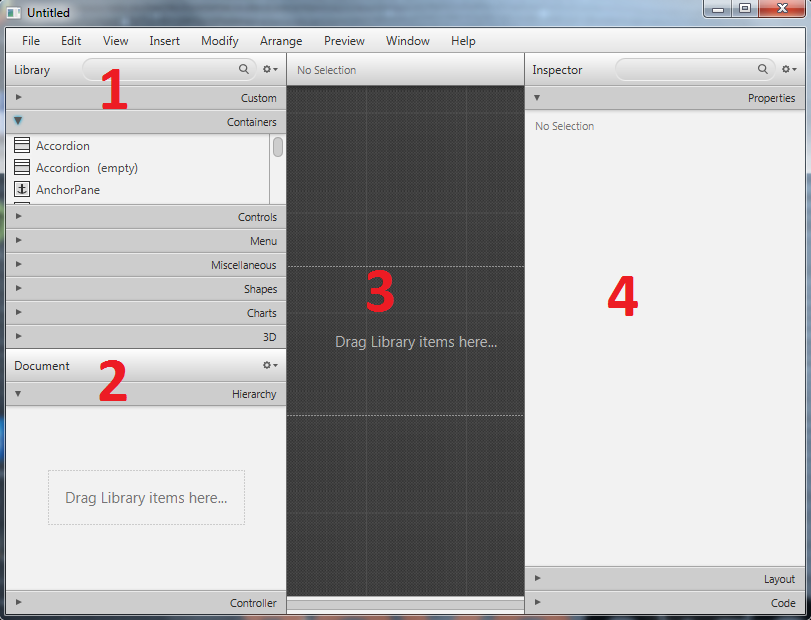
\includegraphics{scenebuilder1.png}\hfill}

W Scene Builderze możemy wyróżnić kilka głównych obszarów roboczych, z których będziemy korzystali. Zgodnie z oznaczeniami na powyższym zrzucie ekranu są to:
\begin{enumerate}
\item {} 
\textbf{Library} -

\item {} 
\textbf{Document} -

\item {} 
\textbf{Podgląd} -

\item {} 
\textbf{Inspector} -

\end{enumerate}

\textbf{Ćwiczenie} \emph{(10 minut)}
\begin{quote}

Zapoznaj się przez chwilę z narzędziem Scene Builder. Spróbuj przeciągnąć różne elementy z sekcji Library do obszaru roboczego lub bezpośrednio do sekcji Document. Kliknij na wybrane z przeciągniętych elementów i spróbuj pozmieniać ustawienia w sekcji Inspector po prawej stronie.
\end{quote}


\subsection{Pierwszy projekt JavaFX}
\label{gui:pierwszy-projekt-javafx}
W celu utworzenia swojego pierwszego projektu w JavieFX przejdź do eclipse i utwórz nowy projekt JavaFX (PPM -\textgreater{} New -\textgreater{} Other -\textgreater{} JavaFX Project).

{\hfill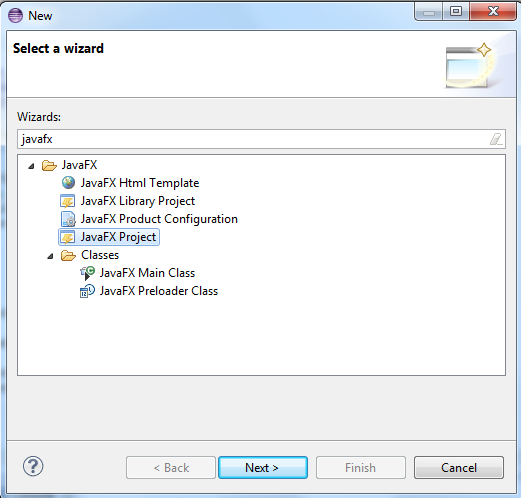
\includegraphics{fx1.png}\hfill}

Następnie wpisz dowolną nazwę projektu i klikając przycisk Next przejdź do ostatniej zakładki kreatora projektu, gdzie wybierz Language jako \textbf{FXML}.

{\hfill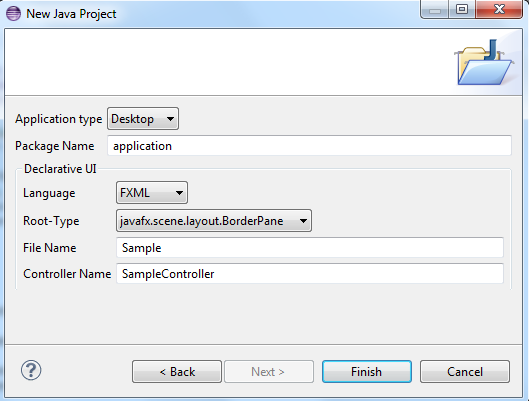
\includegraphics{fx2.png}\hfill}

Wybierz Finish, po czym projekt zostanie utworzony.


\subsection{Omówienie domyślnego projektu}
\label{gui:omowienie-domyslnego-projektu}
Eclipse domyślnie wygeneruje dla nas prosty szablon projektu JavaFX, który już na pierwszy rzut oka różni się od tego co znaliśmy do tej pory.

{\hfill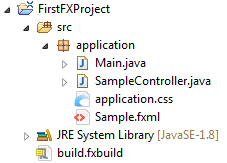
\includegraphics{fxproject.png}\hfill}
\begin{itemize}
\item {} 
Main.java to główna klasa, od której rozpoczyna się działanie aplikacji.

\item {} 
Sample.fxml zawiera definicję tego z jakich layoutów oraz kontrolek zkłada się widok naszej aplikacji - w skrócie jak wygląda

\item {} 
application.css to definicja stylów CSS dla naszej aplikacji. Z pewnością słyszałeś już o nich w przypadku stron internetowych

\item {} 
SampleController.java to dodatkowa klasa, która występuje w architekturze MVC (Model View Controller)

\end{itemize}

\textbf{Model View Controller} jest najpopularniejszym wzorcem architektonicznym wykorzystywanym w tworzeniu aplikacji. Jego głównym zamysłem jest to, żeby oddzielić od siebie definicję tego jak aplikacja wygląda od tego co robi. W komunikacji pomiędzy tymi dwoma elementami występuje kontroler, który odpowiednio przekazuje informacje od użytkownika (GUI aplikacji) do modelu danych i w drugą stronę.

Zaletą takiego podejścia jest to, że aplikacje można rozwijać równolegle i lepiej dzielić obowiązki w zespole programistów. Jeżeli ktoś jest silniejszy tworzeniu tzw. backendu może zająć się programowaniem logiki biznesowej, natomiast osoby o lepszym zmyśle estetycznym mogą się poświęcić stworzeniu frontendu aplikacji.


\subsection{Definiowanie widoku}
\label{gui:definiowanie-widoku}
Widok naszej aplikacji będziemy definiowali w języku XML i formie plików o rozszerzniu .fxml. Na szczęście nie musimy wszystkiego pisać ręcznie, bo kod zostanie wygenerowany na podstawie tego co zrobimy w Scene Builderze.

Żeby przejść do edycji pliku fxml kliknij na niego prawym przyciskiem myszy w eclipse i wybierz opcję Open with SceneBuilder.

{\hfill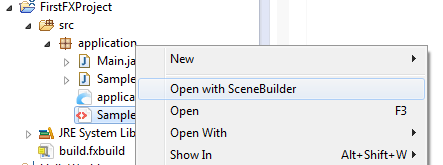
\includegraphics{openwith.png}\hfill}

Jeżeli nic nie zmieniałeś w ustawieniach projektu, to plik Sample.fxml powinien mieć następującą postać:

\emph{plik Sample.fxml}

\begin{Verbatim}[commandchars=\\\{\},numbers=left,firstnumber=1,stepnumber=1]
\PYG{c+cp}{\PYGZlt{}?xml version=\PYGZdq{}1.0\PYGZdq{} encoding=\PYGZdq{}UTF\PYGZhy{}8\PYGZdq{}?\PYGZgt{}}

\PYG{c+cp}{\PYGZlt{}?import javafx.scene.layout.BorderPane?\PYGZgt{}}

\PYG{n+nt}{\PYGZlt{}BorderPane} \PYG{n+na}{xmlns:fx=}\PYG{l+s}{\PYGZdq{}http://javafx.com/fxml\PYGZdq{}} \PYG{n+na}{fx:controller=}\PYG{l+s}{\PYGZdq{}application.SampleController\PYGZdq{}}\PYG{n+nt}{\PYGZgt{}}
    \PYG{c}{\PYGZlt{}!\PYGZhy{}\PYGZhy{}}\PYG{c}{ TODO Add Nodes }\PYG{c}{\PYGZhy{}\PYGZhy{}\PYGZgt{}}
\PYG{n+nt}{\PYGZlt{}/BorderPane\PYGZgt{}}
\end{Verbatim}

\textbf{BorderPane} to główny węzeł naszego widoku. Jest to zwyczajna klasa, którą możesz znaleźć w dokumentacji Javy i której obiekt możesz utworzyć także bezpośrednio w kodzie napisanym w Javie. Jak widzisz klasa ta jest najpierw zaimportowana z pakietu \emph{javafx.scene.layout}. Warto zwrócić uwagę także na atrybut xmlns (skrót od XML Namespace), czyli przestrzeni nazw, z której korzystamy - jeżeli jej nie zdefiniujemy, nasza aplikacja się nie uruchomi, ponieważ kod zostanie uznany za niezgodny ze standardem. atrybut \emph{fx:controller=''application.SampleController''} wskazuje klasę kontrolera powiązaną z tym konkretnym plikiem widoku - w tym przypadku jest to nasza klasa \emph{SampleController}.

W Scene builderze zauważysz, że kod XML ma odzwierciedlenie w sekcji Document Hierarchy, gdzie znajduje się struktura naszego widoku w postaci drzewa węzłów.

{\hfill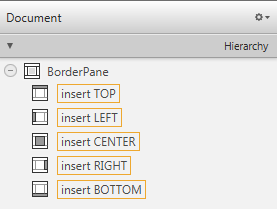
\includegraphics{dochier.png}\hfill}


\subsubsection{Edytor WYSIWYG}
\label{gui:edytor-wysiwyg}
Scene Builder to wygodny wdytor w stylu ``przeciągnij i upuść''. Możesz w nim przeciągnąć kilka kontrolek na nasz główny layout, czyli BorderPane (bezpośrednio do sekcji Document Hierarchy) lub na obszar roboczy. Wszelkie zmiany będą aktualizowane automatycznie.

Spróbujmy teraz zaprojektować bardzo prosty edytor tekstowy, w którym muszą znaleźć się takie elementy jak:
\begin{itemize}
\item {} 
pasek menu kontekstowego

\item {} 
główne pole tekstowe

\item {} 
pasek podliczający ilość wprowadzonych znaków oraz ilość słów w tekście

\end{itemize}

Makieta aplikacji:

{\hfill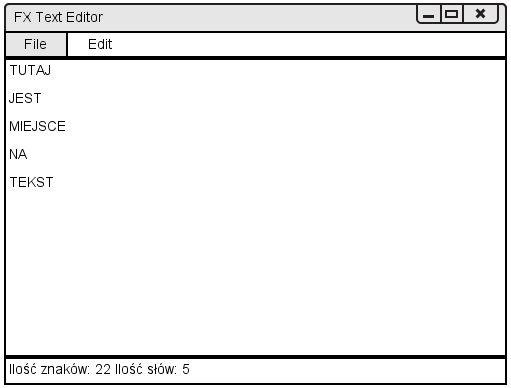
\includegraphics{mockup.png}\hfill}

Struktura projektu eclipse:

{\hfill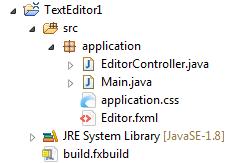
\includegraphics{texteditor.png}\hfill}

Otwórz plik fxml w Scene Builderze i dobierz odpowiednie kontrolki, które umieścisz na głównym layoucie aplikacji (BorderPane). Kontrolki, które należy wykorzystać to:
\begin{itemize}
\item {} 
MenuBar - pasek nawigacyjny, na którym można umieszczać elementy typu MenuItem

\item {} 
TextArea - pole tekstowe, w którym można wprowadzać wiele wierzy tekstu

\item {} 
Label - etykiety tekstowe

\item {} 
Separator - pozwala oddzielić kontrolki od siebie

\end{itemize}

Hierarchia dokumentu FXML w Scene Builderze:

{\hfill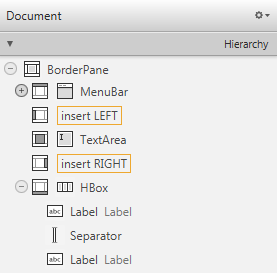
\includegraphics{hierarchy1.png}\hfill}

Jak widzisz etykiety w dolnej części aplikacji opakowane zostały w dodatkowy layout typu HBox.

\begin{notice}{note}{Note:}
Layouty przy tworzeniu graficznego interfejsu użytkownika służą do ustalenia pewnego porządku dodawanych do nich kontrolek. BorderPane pozwala ustawić elementy na krawędziach (góra, dół, lewo, prawo lub środek) natomiast HBox ustawia kontrolki w jednym wierszu jeden obok drugiego. Istnieje dużo więcej layoutów, któe możesz przejrzeć w sekcji containers Scene Buildera. Ikonki umieszczone przy poszczególnych z nich oraz nazwy bardzo dobrze opisują to w jaki sposób możemy je wykorzystać. Layouty mogą być także zagnieżdżane jeden w drugim tak jak w naszym przykładzie, gdzie HBox jest węzłem w layoucie typu BorderPane.
\end{notice}

Problem jaki pojawia się w tym momencie to domyślne parametry kontrolek, które sprawiają, że aplikacja nie wygląda najlepiej:

{\hfill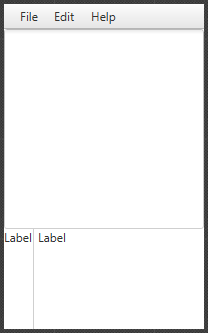
\includegraphics{view1.png}\hfill}

Możemy to na szczęście dosyć łatwo zmodyfikować w sekcji Layout scene buildera (po prawej stronie po kliknięciu na dowolny element), a także wykorzystując opcję dostosowania do domyślnego rozmiaru węzłów potomnych.

Po wcześniejszym zaznaczeniu HBoxa oraz elementów do niego dodanych wybierz opcję Use Computed Sizes, co pozwoli na pozbycie się zbędnej przestrzeni przy naszych etykietach:

{\hfill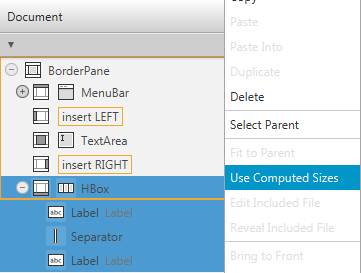
\includegraphics{computedsizes.png}\hfill}

Teraz kliknij na obiekt TextArea i w ustawieniach Layout po prawej stronie ustaw jego wysokość i szerokość (Pref Width i Pref Height):

{\hfill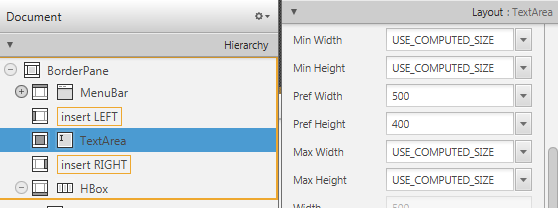
\includegraphics{widthheight.png}\hfill}

W tym momencie po zapisaniu naszego pliku fxml jego kod powinien wyglądać następująco:

\emph{plik Editor.fxml}

\begin{Verbatim}[commandchars=\\\{\},numbers=left,firstnumber=1,stepnumber=1]
\PYG{c+cp}{\PYGZlt{}?xml version=\PYGZdq{}1.0\PYGZdq{} encoding=\PYGZdq{}UTF\PYGZhy{}8\PYGZdq{}?\PYGZgt{}}

\PYG{c+cp}{\PYGZlt{}?import javafx.scene.control.*?\PYGZgt{}}
\PYG{c+cp}{\PYGZlt{}?import java.lang.*?\PYGZgt{}}
\PYG{c+cp}{\PYGZlt{}?import javafx.scene.layout.*?\PYGZgt{}}
\PYG{c+cp}{\PYGZlt{}?import javafx.scene.layout.BorderPane?\PYGZgt{}}

\PYG{n+nt}{\PYGZlt{}BorderPane} \PYG{n+na}{xmlns:fx=}\PYG{l+s}{\PYGZdq{}http://javafx.com/fxml/1\PYGZdq{}} \PYG{n+na}{xmlns=}\PYG{l+s}{\PYGZdq{}http://javafx.com/javafx/8\PYGZdq{}}
    \PYG{n+na}{fx:controller=}\PYG{l+s}{\PYGZdq{}application.SampleController\PYGZdq{}}\PYG{n+nt}{\PYGZgt{}}
    \PYG{n+nt}{\PYGZlt{}top}\PYG{n+nt}{\PYGZgt{}}
        \PYG{n+nt}{\PYGZlt{}MenuBar} \PYG{n+na}{BorderPane.alignment=}\PYG{l+s}{\PYGZdq{}CENTER\PYGZdq{}}\PYG{n+nt}{\PYGZgt{}}
            \PYG{n+nt}{\PYGZlt{}menus}\PYG{n+nt}{\PYGZgt{}}
                \PYG{n+nt}{\PYGZlt{}Menu} \PYG{n+na}{mnemonicParsing=}\PYG{l+s}{\PYGZdq{}false\PYGZdq{}} \PYG{n+na}{text=}\PYG{l+s}{\PYGZdq{}File\PYGZdq{}}\PYG{n+nt}{\PYGZgt{}}
                    \PYG{n+nt}{\PYGZlt{}items}\PYG{n+nt}{\PYGZgt{}}
                        \PYG{n+nt}{\PYGZlt{}MenuItem} \PYG{n+na}{mnemonicParsing=}\PYG{l+s}{\PYGZdq{}false\PYGZdq{}} \PYG{n+na}{text=}\PYG{l+s}{\PYGZdq{}Close\PYGZdq{}} \PYG{n+nt}{/\PYGZgt{}}
                    \PYG{n+nt}{\PYGZlt{}/items\PYGZgt{}}
                \PYG{n+nt}{\PYGZlt{}/Menu\PYGZgt{}}
                \PYG{n+nt}{\PYGZlt{}Menu} \PYG{n+na}{mnemonicParsing=}\PYG{l+s}{\PYGZdq{}false\PYGZdq{}} \PYG{n+na}{text=}\PYG{l+s}{\PYGZdq{}Edit\PYGZdq{}}\PYG{n+nt}{\PYGZgt{}}
                    \PYG{n+nt}{\PYGZlt{}items}\PYG{n+nt}{\PYGZgt{}}
                        \PYG{n+nt}{\PYGZlt{}MenuItem} \PYG{n+na}{mnemonicParsing=}\PYG{l+s}{\PYGZdq{}false\PYGZdq{}} \PYG{n+na}{text=}\PYG{l+s}{\PYGZdq{}Delete\PYGZdq{}} \PYG{n+nt}{/\PYGZgt{}}
                    \PYG{n+nt}{\PYGZlt{}/items\PYGZgt{}}
                \PYG{n+nt}{\PYGZlt{}/Menu\PYGZgt{}}
                \PYG{n+nt}{\PYGZlt{}Menu} \PYG{n+na}{mnemonicParsing=}\PYG{l+s}{\PYGZdq{}false\PYGZdq{}} \PYG{n+na}{text=}\PYG{l+s}{\PYGZdq{}Help\PYGZdq{}}\PYG{n+nt}{\PYGZgt{}}
                    \PYG{n+nt}{\PYGZlt{}items}\PYG{n+nt}{\PYGZgt{}}
                        \PYG{n+nt}{\PYGZlt{}MenuItem} \PYG{n+na}{mnemonicParsing=}\PYG{l+s}{\PYGZdq{}false\PYGZdq{}} \PYG{n+na}{text=}\PYG{l+s}{\PYGZdq{}About\PYGZdq{}} \PYG{n+nt}{/\PYGZgt{}}
                    \PYG{n+nt}{\PYGZlt{}/items\PYGZgt{}}
                \PYG{n+nt}{\PYGZlt{}/Menu\PYGZgt{}}
            \PYG{n+nt}{\PYGZlt{}/menus\PYGZgt{}}
        \PYG{n+nt}{\PYGZlt{}/MenuBar\PYGZgt{}}
    \PYG{n+nt}{\PYGZlt{}/top\PYGZgt{}}
    \PYG{n+nt}{\PYGZlt{}center}\PYG{n+nt}{\PYGZgt{}}
        \PYG{n+nt}{\PYGZlt{}TextArea} \PYG{n+na}{prefHeight=}\PYG{l+s}{\PYGZdq{}400.0\PYGZdq{}} \PYG{n+na}{prefWidth=}\PYG{l+s}{\PYGZdq{}500.0\PYGZdq{}}
            \PYG{n+na}{BorderPane.alignment=}\PYG{l+s}{\PYGZdq{}CENTER\PYGZdq{}} \PYG{n+nt}{/\PYGZgt{}}
    \PYG{n+nt}{\PYGZlt{}/center\PYGZgt{}}
    \PYG{n+nt}{\PYGZlt{}bottom}\PYG{n+nt}{\PYGZgt{}}
        \PYG{n+nt}{\PYGZlt{}HBox} \PYG{n+na}{BorderPane.alignment=}\PYG{l+s}{\PYGZdq{}CENTER\PYGZdq{}}\PYG{n+nt}{\PYGZgt{}}
            \PYG{n+nt}{\PYGZlt{}children}\PYG{n+nt}{\PYGZgt{}}
                \PYG{n+nt}{\PYGZlt{}Label} \PYG{n+na}{text=}\PYG{l+s}{\PYGZdq{}Label\PYGZdq{}} \PYG{n+nt}{/\PYGZgt{}}
                \PYG{n+nt}{\PYGZlt{}Separator} \PYG{n+na}{orientation=}\PYG{l+s}{\PYGZdq{}VERTICAL\PYGZdq{}} \PYG{n+nt}{/\PYGZgt{}}
                \PYG{n+nt}{\PYGZlt{}Label} \PYG{n+na}{text=}\PYG{l+s}{\PYGZdq{}Label\PYGZdq{}} \PYG{n+nt}{/\PYGZgt{}}
            \PYG{n+nt}{\PYGZlt{}/children\PYGZgt{}}
        \PYG{n+nt}{\PYGZlt{}/HBox\PYGZgt{}}
    \PYG{n+nt}{\PYGZlt{}/bottom\PYGZgt{}}
\PYG{n+nt}{\PYGZlt{}/BorderPane\PYGZgt{}}
\end{Verbatim}

Jak widać każdy element, który dodaliśmy w Scene Builderze ma tutaj swoje odzwierciedlenie w postaci węxła XML. Widoczne są także ustawienia poszczególnych elementów, np. wysokość i szerokość TextArea postaci \emph{TextArea prefHeight=''400.0'' prefWidth=''500.0''}.

W tym momencie warto zobaczyć jak nasza aplikacja będzie wyglądała po uruchomieniu. Co ciekawe jeżeli chcemy podejrzeć tylko wygląd bez funkcjonalności, możemy to zrobić bezpośrednio z poziomu Scene Buildera korzystając z opcji Preview -\textgreater{} Show Preview in Window (Ctrl + P).

{\hfill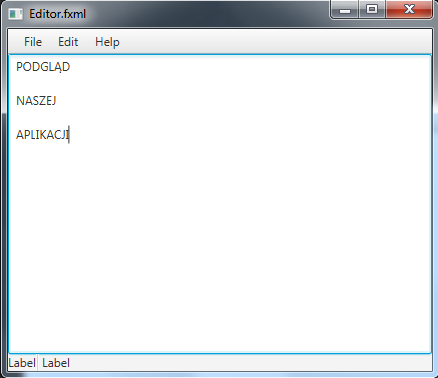
\includegraphics{preview.png}\hfill}

Jak widzisz widok aplikacji można więc definiować nawet nie znając języka Java.


\subsection{Architektura aplikacji}
\label{gui:architektura-aplikacji}
Czas wrócić jednak do tego, aby nasza aplikacja dała się uruchomić z poziomu eclipse jako aplikacja Javy. Zacznijmy od poprawki w nazwie pliku fxml wczytywanym w klasie Main:

\begin{Verbatim}[commandchars=\\\{\},numbers=left,firstnumber=1,stepnumber=1]
\PYG{k+kn}{package} \PYG{n}{application}\PYG{o}{;}

\PYG{k+kn}{import} \PYG{n+nn}{javafx.application.Application}\PYG{o}{;}
\PYG{k+kn}{import} \PYG{n+nn}{javafx.fxml.FXMLLoader}\PYG{o}{;}
\PYG{k+kn}{import} \PYG{n+nn}{javafx.scene.Scene}\PYG{o}{;}
\PYG{k+kn}{import} \PYG{n+nn}{javafx.scene.layout.BorderPane}\PYG{o}{;}
\PYG{k+kn}{import} \PYG{n+nn}{javafx.stage.Stage}\PYG{o}{;}

\PYG{k+kd}{public} \PYG{k+kd}{class} \PYG{n+nc}{Main} \PYG{k+kd}{extends} \PYG{n}{Application} \PYG{o}{\PYGZob{}}
    \PYG{n+nd}{@Override}
    \PYG{k+kd}{public} \PYG{k+kt}{void} \PYG{n+nf}{start}\PYG{o}{(}\PYG{n}{Stage} \PYG{n}{primaryStage}\PYG{o}{)} \PYG{o}{\PYGZob{}}
        \PYG{k}{try} \PYG{o}{\PYGZob{}}
            \PYG{n}{BorderPane} \PYG{n}{root} \PYG{o}{=} \PYG{o}{(}\PYG{n}{BorderPane}\PYG{o}{)} \PYG{n}{FXMLLoader}\PYG{o}{.}\PYG{n+na}{load}\PYG{o}{(}\PYG{n}{getClass}\PYG{o}{(}\PYG{o}{)}
                    \PYG{o}{.}\PYG{n+na}{getResource}\PYG{o}{(}\PYG{l+s}{\PYGZdq{}Editor.fxml\PYGZdq{}}\PYG{o}{)}\PYG{o}{)}\PYG{o}{;}
            \PYG{n}{Scene} \PYG{n}{scene} \PYG{o}{=} \PYG{k}{new} \PYG{n}{Scene}\PYG{o}{(}\PYG{n}{root}\PYG{o}{,} \PYG{l+m+mi}{400}\PYG{o}{,} \PYG{l+m+mi}{400}\PYG{o}{)}\PYG{o}{;}
            \PYG{n}{scene}\PYG{o}{.}\PYG{n+na}{getStylesheets}\PYG{o}{(}\PYG{o}{)}\PYG{o}{.}\PYG{n+na}{add}\PYG{o}{(}
                    \PYG{n}{getClass}\PYG{o}{(}\PYG{o}{)}\PYG{o}{.}\PYG{n+na}{getResource}\PYG{o}{(}\PYG{l+s}{\PYGZdq{}application.css\PYGZdq{}}\PYG{o}{)}\PYG{o}{.}\PYG{n+na}{toExternalForm}\PYG{o}{(}\PYG{o}{)}\PYG{o}{)}\PYG{o}{;}
            \PYG{n}{primaryStage}\PYG{o}{.}\PYG{n+na}{setScene}\PYG{o}{(}\PYG{n}{scene}\PYG{o}{)}\PYG{o}{;}
            \PYG{n}{primaryStage}\PYG{o}{.}\PYG{n+na}{show}\PYG{o}{(}\PYG{o}{)}\PYG{o}{;}
        \PYG{o}{\PYGZcb{}} \PYG{k}{catch} \PYG{o}{(}\PYG{n}{Exception} \PYG{n}{e}\PYG{o}{)} \PYG{o}{\PYGZob{}}
            \PYG{n}{e}\PYG{o}{.}\PYG{n+na}{printStackTrace}\PYG{o}{(}\PYG{o}{)}\PYG{o}{;}
        \PYG{o}{\PYGZcb{}}
    \PYG{o}{\PYGZcb{}}

    \PYG{k+kd}{public} \PYG{k+kd}{static} \PYG{k+kt}{void} \PYG{n+nf}{main}\PYG{o}{(}\PYG{n}{String}\PYG{o}{[}\PYG{o}{]} \PYG{n}{args}\PYG{o}{)} \PYG{o}{\PYGZob{}}
        \PYG{n}{launch}\PYG{o}{(}\PYG{n}{args}\PYG{o}{)}\PYG{o}{;}
    \PYG{o}{\PYGZcb{}}
\PYG{o}{\PYGZcb{}}
\end{Verbatim}

Omówmy ten kod linijka po linijce:
\begin{enumerate}
\item {} 
Wiersze 1-8 to deklaracja pakietu oraz import bibliotek, które później wykorzystujemy

\item {} 
W linijce 9 widzimy, że nasza klasa Main rozszerza klasę Application. Oznacza to, że jest to główna klasa aplikacji napisanej w JavieFX i to od niej rozpocznie się działanie naszej aplikacji.

\item {} 
Klasa Application posiada jedną abstrakcyjną metodę \emph{start()}, którą musimy przesłonić (Override). Jako jej argument przekazany zostanie obiekt Stage, który zostanie utworzony przez wirtualną maszynę. \textbf{Stage} to okno naszej aplikacji.

\item {} 
W wierszach 13-14 wczytujemy nasz widok za pomocą specjalnej klasy FXMLLoader i metody \emph{load()}. Przetwarza ona plik XML i na podstawie zawartych w nim definicji tworzy obiekty, które będą odzwierciedlone w kodzie Javy.

\item {} 
W 15 wierzu tworzymy obiekt \textbf{Scene}, który dodamy do naszego okna (Stage) w wierszu 18. Scene to klasa reprezentująca główny kontener z widokiem aplikacji, do któego możemy dodawać inne elementy takie jak layouty, czy konkretne kontrolki.

\item {} 
W 16 i 17 wierzu wczytujemy style CSS, które aplikujemy do naszej sceny. Ponieważ na tę chwilę plik \emph{application.css} jest pusty, nie będzie to miało wpływu na wygląd naszej aplikacji.

\item {} 
W metodzie \emph{main()} wywołujemy metodę \emph{launch()} ta z kolei odpowiada za cykl życia aplikacji JavaFX, czyli m.in. wywołanie metody \emph{start()}.

\end{enumerate}

Ostateczna hierarchia widoku w JavieFX wygląda więc następująco:

{\hfill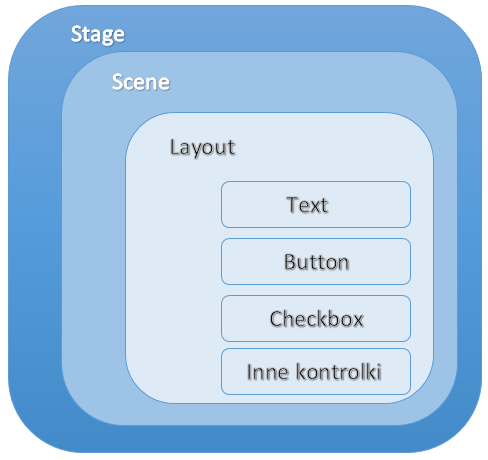
\includegraphics{viewh.png}\hfill}

Pozostaje nam jeszcze jedna rzecz do poprawy. Przy próbie uruchomienia programu otrzymujemy błąd \emph{Caused by: java.lang.ClassNotFoundException: application.SampleController} - jest on spowodowany tym, że w pliku fxml nie zmieniliśmy klasy kontrolera (fx:controller) po zmianie nazwy pliku z klasą (EditorController).

W Scene Builderze można to zrobić także w sekcji Document rozwijając zakładkę Controller. Nazwę klasy kontrolera należy podać również ze ścieżką uwzględniającą pakiet (tzw. fully qualified name).

{\hfill\includegraphics{fxcontroller.png}\hfill}

Definicja BorderPane w pliku fxml powinna więc wyglądać teraz następująco:

\begin{Verbatim}[commandchars=\\\{\},numbers=left,firstnumber=1,stepnumber=1]
\PYG{n+nt}{\PYGZlt{}BorderPane} \PYG{n+na}{xmlns=}\PYG{l+s}{\PYGZdq{}http://javafx.com/javafx/8\PYGZdq{}} \PYG{n+na}{xmlns:fx=}\PYG{l+s}{\PYGZdq{}http://javafx.com/fxml/1\PYGZdq{}}
    \PYG{n+na}{fx:controller=}\PYG{l+s}{\PYGZdq{}application.EditorController\PYGZdq{}}\PYG{n+nt}{\PYGZgt{}}
\end{Verbatim}

W tym momencie powinniśmy mieć już możliwość uruchomienia naszej aplikacji z poziomu eclipse a naszym oczom powinien ukazać się widok analogiczny do podglądu, który widzieliśmy wcześniej w Scene Builderze.

\begin{notice}{attention}{Attention:}
Jeżeli przy próbie uruchomienia aplikacji nadal pojawia się jakiś błąd związany z dokumentem fxml, a jesteś pewny, że zapisałeś go w Scene Builderze, otwórz go w eclipse, a to pomoże go odświeżyć. Jeżeli nie otworzysz pliku, który przed chwilą edytowałeś w innym edytorze, eclipse może korzystać ze starszej wersji dokumentu, który wczytał już do pamięci.
\end{notice}


\subsection{FXML a klasa kontrolera}
\label{gui:fxml-a-klasa-kontrolera}
Nasza aplikacja daje się już w tym momencie uruchomić, jednak w żaden sposób nie możemy odwołać się do pola tekstowego w naszym kodzie Javy. Zgodnie z architekturą MVC powinniśmy móc pobierać i wysyłać informacje do kontrolek zdefiniowanych w widoku poprzez klasę kontrolera. W tym celu musimy zdefiniować w dokumencie fxml dodatkowe atrybuty \textbf{fx:id} dla każdej z kontrolek, a najłatwiej będzie to zrobić przełączając najpierw widok w sekcji Document Hierarchy na fx:id właśnie.

{\hfill\includegraphics{fxid.png}\hfill}

Nadając fx:id pamiętaj, żeby były to znaczące nazwy, ponieważ będą to jednocześnie nazwy zmiennych w kodzie Javy. fx:id ustawić klikając dwukrotnie obok danej kontrolki w sekcji Document Hierarchy lub wprowadzając ją w sekcji Code (prawe menu).

{\hfill\includegraphics{fxid2.png}\hfill}

Teraz w klasie ustawionej jako fx:controller należy utworzyć zmienne odpowiadające odpowiednim typom kontrolek i nadać im nazwy zgodne z ustalonymi przed chwilą fx:id. Na szczęście nie trzeba tego robić ręcznie. Przejdź w Scene Builderze to sekcji \textbf{View -\textgreater{} Show sample controller skeleton} skopiuj przykładowy kod i wklej go do pliku EditorController w eclipse.

W JavieFX ogólnie przyjętą praktyką jest także implementowanie interfejsu \textbf{Initializable} przez klasę kontrolera. Interfejs ten wymusi zaimplementowanie metody initialize(), która zostanie wywołana w momencie uruchamiania aplikacji przez FXMLLoadera.

\emph{plik EditorController.java}

\begin{Verbatim}[commandchars=\\\{\},numbers=left,firstnumber=1,stepnumber=1]
\PYG{k+kn}{package} \PYG{n}{application}\PYG{o}{;}

\PYG{k+kn}{import} \PYG{n+nn}{java.net.URL}\PYG{o}{;}
\PYG{k+kn}{import} \PYG{n+nn}{java.util.ResourceBundle}\PYG{o}{;}

\PYG{k+kn}{import} \PYG{n+nn}{javafx.fxml.FXML}\PYG{o}{;}
\PYG{k+kn}{import} \PYG{n+nn}{javafx.fxml.Initializable}\PYG{o}{;}
\PYG{k+kn}{import} \PYG{n+nn}{javafx.scene.control.Label}\PYG{o}{;}
\PYG{k+kn}{import} \PYG{n+nn}{javafx.scene.control.TextArea}\PYG{o}{;}

\PYG{k+kd}{public} \PYG{k+kd}{class} \PYG{n+nc}{EditorController} \PYG{k+kd}{implements} \PYG{n}{Initializable} \PYG{o}{\PYGZob{}}

    \PYG{n+nd}{@FXML}
    \PYG{k+kd}{private} \PYG{n}{TextArea} \PYG{n}{mainTextArea}\PYG{o}{;}

    \PYG{n+nd}{@FXML}
    \PYG{k+kd}{private} \PYG{n}{Label} \PYG{n}{wordsCountLabel}\PYG{o}{;}

    \PYG{n+nd}{@FXML}
    \PYG{k+kd}{private} \PYG{n}{Label} \PYG{n}{lettersCountLabel}\PYG{o}{;}

    \PYG{n+nd}{@Override}
    \PYG{k+kd}{public} \PYG{k+kt}{void} \PYG{n+nf}{initialize}\PYG{o}{(}\PYG{n}{URL} \PYG{n}{arg0}\PYG{o}{,} \PYG{n}{ResourceBundle} \PYG{n}{arg1}\PYG{o}{)} \PYG{o}{\PYGZob{}}
        \PYG{c+c1}{// TODO Auto\PYGZhy{}generated method stub}

    \PYG{o}{\PYGZcb{}}
\PYG{o}{\PYGZcb{}}
\end{Verbatim}


\subsection{Odwołanie do kontrolek z kodu Javy}
\label{gui:odwolanie-do-kontrolek-z-kodu-javy}
Ostatni etap w tej lekcji to odwoływanie się do kontrolek zdefiniowanych w FXMLu z poziomu klasy kontrolera w kodzie Javy. Tak jak wspomnieliśmy przy wprowadzeniu do Javy FX, kontrolki to tak naprawdę nic innego niż zwykłe klasy Javy. Stworzyliśmy je w sposób deklaratywny w kodzie XML, jednak następnie obiekty zostały wstrzyknięte do klasy kontrolera i tam mamy już do nich dostęp, więc możemy na nich wywoływać odpowiednie metody.

W metodzie initialize() ustawmy tekst naszego głównego pola tekstowego oraz etykiet, aby zweryfikować, że ustawione przez nas fx:id zostały poprawnie powiązane ze zmiennymi.

\emph{plik EditorController.java}

\begin{Verbatim}[commandchars=\\\{\},numbers=left,firstnumber=1,stepnumber=1]
\PYG{k+kn}{package} \PYG{n}{application}\PYG{o}{;}

\PYG{k+kn}{import} \PYG{n+nn}{java.net.URL}\PYG{o}{;}
\PYG{k+kn}{import} \PYG{n+nn}{java.util.ResourceBundle}\PYG{o}{;}

\PYG{k+kn}{import} \PYG{n+nn}{javafx.fxml.FXML}\PYG{o}{;}
\PYG{k+kn}{import} \PYG{n+nn}{javafx.fxml.Initializable}\PYG{o}{;}
\PYG{k+kn}{import} \PYG{n+nn}{javafx.scene.control.Label}\PYG{o}{;}
\PYG{k+kn}{import} \PYG{n+nn}{javafx.scene.control.TextArea}\PYG{o}{;}

\PYG{k+kd}{public} \PYG{k+kd}{class} \PYG{n+nc}{EditorController} \PYG{k+kd}{implements} \PYG{n}{Initializable} \PYG{o}{\PYGZob{}}

    \PYG{n+nd}{@FXML}
    \PYG{k+kd}{private} \PYG{n}{TextArea} \PYG{n}{mainTextArea}\PYG{o}{;}

    \PYG{n+nd}{@FXML}
    \PYG{k+kd}{private} \PYG{n}{Label} \PYG{n}{wordsCountLabel}\PYG{o}{;}

    \PYG{n+nd}{@FXML}
    \PYG{k+kd}{private} \PYG{n}{Label} \PYG{n}{lettersCountLabel}\PYG{o}{;}

    \PYG{n+nd}{@Override}
    \PYG{k+kd}{public} \PYG{k+kt}{void} \PYG{n+nf}{initialize}\PYG{o}{(}\PYG{n}{URL} \PYG{n}{arg0}\PYG{o}{,} \PYG{n}{ResourceBundle} \PYG{n}{arg1}\PYG{o}{)} \PYG{o}{\PYGZob{}}
        \PYG{n}{String} \PYG{n}{mainText} \PYG{o}{=} \PYG{l+s}{\PYGZdq{}To jest długi tekst,\PYGZbs{}n\PYGZdq{}}
                \PYG{o}{+} \PYG{l+s}{\PYGZdq{}który zostanie wyświetlony\PYGZbs{}n\PYGZdq{}}
                \PYG{o}{+} \PYG{l+s}{\PYGZdq{}w głównym oknie aplikacji\PYGZdq{}}\PYG{o}{;}
        \PYG{n}{String} \PYG{n}{letters} \PYG{o}{=} \PYG{l+s}{\PYGZdq{}Ilość liter: 50\PYGZdq{}}\PYG{o}{;}
        \PYG{n}{String} \PYG{n}{words} \PYG{o}{=} \PYG{l+s}{\PYGZdq{}Ilość słów: 12\PYGZdq{}}\PYG{o}{;}

        \PYG{n}{mainTextArea}\PYG{o}{.}\PYG{n+na}{setText}\PYG{o}{(}\PYG{n}{mainText}\PYG{o}{)}\PYG{o}{;}
        \PYG{n}{lettersCountLabel}\PYG{o}{.}\PYG{n+na}{setText}\PYG{o}{(}\PYG{n}{letters}\PYG{o}{)}\PYG{o}{;}
        \PYG{n}{wordsCountLabel}\PYG{o}{.}\PYG{n+na}{setText}\PYG{o}{(}\PYG{n}{words}\PYG{o}{)}\PYG{o}{;}
    \PYG{o}{\PYGZcb{}}
\PYG{o}{\PYGZcb{}}
\end{Verbatim}

W wierszach 30-32 ustawiamy teksty odpowiednich kontrolek za pomocą metod \emph{setText()}. Analogicznie w celu odczytania tekstu, który wprowadzi użytkownik będziemy używali metody \emph{getText()}, jednak tego nauczymy się już w kolejnej lekcji omawiając obsługę zdarzeń.

Adnotacja @FXML

{\hfill\includegraphics{end.png}\hfill}

\href{http://javafxports.org/page/What\_is\_JavaFXPorts}{http://javafxports.org/page/What\_is\_JavaFXPorts}


\section{Graficzny interfejs użytkownika cz.2}
\label{gui2:graficzny-interfejs-uzytkownika-cz-2}\label{gui2::doc}
W tej lekcji dowiesz się:
\begin{itemize}
\item {} 
w jaki sposó obsługiwać zdarzenia przycisków

\item {} 
jak dodać dodać obsługę zdarzeń myszy lub klawiatury

\item {} 
czym są klasy anonimowe

\end{itemize}


\subsection{Obsługa zdarzeń}
\label{gui2:obsluga-zdarzen}
W poprzedniej lekcji dowiedziałeś się w jaki sposób stworzyć prosty graficzny interfejs użytkownika korzystając z Javy FX, na czym polega architektura MVC i jak powiązać kontrolki zdefiniowane w pliku fxml ze zmiennymi w klasie kontrolera, a także jak z poziomu kodu Javy ustawiać ich właściwości na przykładzie metody \emph{setText()}.

Problemem jest jednak to, że zdefiniowane menu nawigacyjne nie reaguje w żaden sposób na akcje wykonywane przez użytkownika, zliczanie słów oraz wyrazów także jest zakodowane na sztywno i nie reaguje na to co użytkownik wprowadza do pola tekstowego.

Rozwiązaniem tych problemów jest podpięcie pod poszczególne z kontrolek odpowiednich zdarzeń, które w odpowiedzi wykonają pewną akcję. Istnieje kilka metod na realizację tego zadania, jednak my skupimy się na dwóch.


\subsection{Podpięcie zdarzeń przycisków}
\label{gui2:podpiecie-zdarzen-przyciskow}
Jednymi z najczęściej powtarzających się opcji w niemal każdej aplikacji jest odpowiedź aplikacji na akcję użytkownika polegającą na wciśnięcie zwykłęgo przycisku (w JavieFX reprezentowany przez klasę Button). W naszym przykładowym programie nie posiadamy na tę chwilę żadnego przycisku, jednak nic nie stoi na przeszkodzie, żeby go dodać.

\emph{hierarchia Editor.fxml}

{\hfill\includegraphics{button-hierarchy.png}\hfill}

\emph{plik Editor.fxml}

\begin{Verbatim}[commandchars=\\\{\},numbers=left,firstnumber=1,stepnumber=1]
\PYG{c+cp}{\PYGZlt{}?xml version=\PYGZdq{}1.0\PYGZdq{} encoding=\PYGZdq{}UTF\PYGZhy{}8\PYGZdq{}?\PYGZgt{}}

\PYG{c+cp}{\PYGZlt{}?import javafx.scene.control.*?\PYGZgt{}}
\PYG{c+cp}{\PYGZlt{}?import java.lang.*?\PYGZgt{}}
\PYG{c+cp}{\PYGZlt{}?import javafx.scene.layout.*?\PYGZgt{}}
\PYG{c+cp}{\PYGZlt{}?import javafx.scene.layout.BorderPane?\PYGZgt{}}

\PYG{n+nt}{\PYGZlt{}BorderPane} \PYG{n+na}{xmlns=}\PYG{l+s}{\PYGZdq{}http://javafx.com/javafx/8\PYGZdq{}} \PYG{n+na}{xmlns:fx=}\PYG{l+s}{\PYGZdq{}http://javafx.com/fxml/1\PYGZdq{}}
    \PYG{n+na}{fx:controller=}\PYG{l+s}{\PYGZdq{}application.EditorController\PYGZdq{}}\PYG{n+nt}{\PYGZgt{}}
    \PYG{n+nt}{\PYGZlt{}top}\PYG{n+nt}{\PYGZgt{}}
        \PYG{n+nt}{\PYGZlt{}MenuBar} \PYG{n+na}{BorderPane.alignment=}\PYG{l+s}{\PYGZdq{}CENTER\PYGZdq{}}\PYG{n+nt}{\PYGZgt{}}
            \PYG{n+nt}{\PYGZlt{}menus}\PYG{n+nt}{\PYGZgt{}}
                \PYG{n+nt}{\PYGZlt{}Menu} \PYG{n+na}{mnemonicParsing=}\PYG{l+s}{\PYGZdq{}false\PYGZdq{}} \PYG{n+na}{text=}\PYG{l+s}{\PYGZdq{}File\PYGZdq{}}\PYG{n+nt}{\PYGZgt{}}
                    \PYG{n+nt}{\PYGZlt{}items}\PYG{n+nt}{\PYGZgt{}}
                        \PYG{n+nt}{\PYGZlt{}MenuItem} \PYG{n+na}{mnemonicParsing=}\PYG{l+s}{\PYGZdq{}false\PYGZdq{}} \PYG{n+na}{text=}\PYG{l+s}{\PYGZdq{}Close\PYGZdq{}} \PYG{n+nt}{/\PYGZgt{}}
                    \PYG{n+nt}{\PYGZlt{}/items\PYGZgt{}}
                \PYG{n+nt}{\PYGZlt{}/Menu\PYGZgt{}}
                \PYG{n+nt}{\PYGZlt{}Menu} \PYG{n+na}{mnemonicParsing=}\PYG{l+s}{\PYGZdq{}false\PYGZdq{}} \PYG{n+na}{text=}\PYG{l+s}{\PYGZdq{}Edit\PYGZdq{}}\PYG{n+nt}{\PYGZgt{}}
                    \PYG{n+nt}{\PYGZlt{}items}\PYG{n+nt}{\PYGZgt{}}
                        \PYG{n+nt}{\PYGZlt{}MenuItem} \PYG{n+na}{mnemonicParsing=}\PYG{l+s}{\PYGZdq{}false\PYGZdq{}} \PYG{n+na}{text=}\PYG{l+s}{\PYGZdq{}Delete\PYGZdq{}} \PYG{n+nt}{/\PYGZgt{}}
                    \PYG{n+nt}{\PYGZlt{}/items\PYGZgt{}}
                \PYG{n+nt}{\PYGZlt{}/Menu\PYGZgt{}}
                \PYG{n+nt}{\PYGZlt{}Menu} \PYG{n+na}{mnemonicParsing=}\PYG{l+s}{\PYGZdq{}false\PYGZdq{}} \PYG{n+na}{text=}\PYG{l+s}{\PYGZdq{}Help\PYGZdq{}}\PYG{n+nt}{\PYGZgt{}}
                    \PYG{n+nt}{\PYGZlt{}items}\PYG{n+nt}{\PYGZgt{}}
                        \PYG{n+nt}{\PYGZlt{}MenuItem} \PYG{n+na}{mnemonicParsing=}\PYG{l+s}{\PYGZdq{}false\PYGZdq{}} \PYG{n+na}{text=}\PYG{l+s}{\PYGZdq{}About\PYGZdq{}} \PYG{n+nt}{/\PYGZgt{}}
                    \PYG{n+nt}{\PYGZlt{}/items\PYGZgt{}}
                \PYG{n+nt}{\PYGZlt{}/Menu\PYGZgt{}}
            \PYG{n+nt}{\PYGZlt{}/menus\PYGZgt{}}
        \PYG{n+nt}{\PYGZlt{}/MenuBar\PYGZgt{}}
    \PYG{n+nt}{\PYGZlt{}/top\PYGZgt{}}
    \PYG{n+nt}{\PYGZlt{}center}\PYG{n+nt}{\PYGZgt{}}
        \PYG{n+nt}{\PYGZlt{}TextArea} \PYG{n+na}{fx:id=}\PYG{l+s}{\PYGZdq{}mainTextArea\PYGZdq{}} \PYG{n+na}{prefHeight=}\PYG{l+s}{\PYGZdq{}400.0\PYGZdq{}} \PYG{n+na}{prefWidth=}\PYG{l+s}{\PYGZdq{}500.0\PYGZdq{}}
            \PYG{n+na}{BorderPane.alignment=}\PYG{l+s}{\PYGZdq{}CENTER\PYGZdq{}} \PYG{n+nt}{/\PYGZgt{}}
    \PYG{n+nt}{\PYGZlt{}/center\PYGZgt{}}
    \PYG{n+nt}{\PYGZlt{}bottom}\PYG{n+nt}{\PYGZgt{}}
        \PYG{n+nt}{\PYGZlt{}HBox} \PYG{n+na}{alignment=}\PYG{l+s}{\PYGZdq{}CENTER\PYGZus{}LEFT\PYGZdq{}} \PYG{n+na}{BorderPane.alignment=}\PYG{l+s}{\PYGZdq{}CENTER\PYGZdq{}}\PYG{n+nt}{\PYGZgt{}}
            \PYG{n+nt}{\PYGZlt{}children}\PYG{n+nt}{\PYGZgt{}}
                \PYG{n+nt}{\PYGZlt{}Label} \PYG{n+na}{fx:id=}\PYG{l+s}{\PYGZdq{}lettersCountLabel\PYGZdq{}} \PYG{n+na}{text=}\PYG{l+s}{\PYGZdq{}Label\PYGZdq{}} \PYG{n+nt}{/\PYGZgt{}}
                \PYG{n+nt}{\PYGZlt{}Separator} \PYG{n+na}{orientation=}\PYG{l+s}{\PYGZdq{}VERTICAL\PYGZdq{}} \PYG{n+nt}{/\PYGZgt{}}
                \PYG{n+nt}{\PYGZlt{}Label} \PYG{n+na}{fx:id=}\PYG{l+s}{\PYGZdq{}wordsCountLabel\PYGZdq{}} \PYG{n+na}{text=}\PYG{l+s}{\PYGZdq{}Label\PYGZdq{}} \PYG{n+nt}{/\PYGZgt{}}
                \PYG{n+nt}{\PYGZlt{}Separator} \PYG{n+na}{orientation=}\PYG{l+s}{\PYGZdq{}VERTICAL\PYGZdq{}} \PYG{n+nt}{/\PYGZgt{}}
                \PYG{n+nt}{\PYGZlt{}Button} \PYG{n+na}{fx:id=}\PYG{l+s}{\PYGZdq{}clearButton\PYGZdq{}} \PYG{n+na}{mnemonicParsing=}\PYG{l+s}{\PYGZdq{}false\PYGZdq{}} \PYG{n+na}{text=}\PYG{l+s}{\PYGZdq{}Clear\PYGZdq{}} \PYG{n+nt}{/\PYGZgt{}}
            \PYG{n+nt}{\PYGZlt{}/children\PYGZgt{}}
        \PYG{n+nt}{\PYGZlt{}/HBox\PYGZgt{}}
    \PYG{n+nt}{\PYGZlt{}/bottom\PYGZgt{}}
\PYG{n+nt}{\PYGZlt{}/BorderPane\PYGZgt{}}
\end{Verbatim}

Przycisk dodaliśmy w dolnej części aplikacji ustawiając na nim domyślny tekst ``Clear'' oraz nadając fx:id \emph{clearButton} - posłuży on nam do wyczyszczenia zawartości pola tekstowego.

Musimy także zdefiniować zmienną odpowiadającą fx:id przycisku w klasie kontrolera, abyśmy mogli dodać do niego obsługę zdarzenia. Robimy to używając adnotacji @FXML i nazwy zmiennej zgodnej z fx:id.

\emph{plik EditorController.java}

\begin{Verbatim}[commandchars=\\\{\},numbers=left,firstnumber=1,stepnumber=1]
\PYG{k+kn}{package} \PYG{n}{application}\PYG{o}{;}

\PYG{k+kn}{import} \PYG{n+nn}{java.net.URL}\PYG{o}{;}
\PYG{k+kn}{import} \PYG{n+nn}{java.util.ResourceBundle}\PYG{o}{;}

\PYG{k+kn}{import} \PYG{n+nn}{javafx.fxml.FXML}\PYG{o}{;}
\PYG{k+kn}{import} \PYG{n+nn}{javafx.fxml.Initializable}\PYG{o}{;}
\PYG{k+kn}{import} \PYG{n+nn}{javafx.scene.control.Button}\PYG{o}{;}
\PYG{k+kn}{import} \PYG{n+nn}{javafx.scene.control.Label}\PYG{o}{;}
\PYG{k+kn}{import} \PYG{n+nn}{javafx.scene.control.TextArea}\PYG{o}{;}

\PYG{k+kd}{public} \PYG{k+kd}{class} \PYG{n+nc}{EditorController} \PYG{k+kd}{implements} \PYG{n}{Initializable} \PYG{o}{\PYGZob{}}

    \PYG{n+nd}{@FXML}
    \PYG{k+kd}{private} \PYG{n}{TextArea} \PYG{n}{mainTextArea}\PYG{o}{;}

    \PYG{n+nd}{@FXML}
    \PYG{k+kd}{private} \PYG{n}{Label} \PYG{n}{wordsCountLabel}\PYG{o}{;}

    \PYG{n+nd}{@FXML}
    \PYG{k+kd}{private} \PYG{n}{Label} \PYG{n}{lettersCountLabel}\PYG{o}{;}

    \PYG{n+nd}{@FXML}
    \PYG{k+kd}{private} \PYG{n}{Button} \PYG{n}{clearButton}\PYG{o}{;}

    \PYG{n+nd}{@Override}
    \PYG{k+kd}{public} \PYG{k+kt}{void} \PYG{n+nf}{initialize}\PYG{o}{(}\PYG{n}{URL} \PYG{n}{arg0}\PYG{o}{,} \PYG{n}{ResourceBundle} \PYG{n}{arg1}\PYG{o}{)} \PYG{o}{\PYGZob{}}
        \PYG{n}{String} \PYG{n}{mainText} \PYG{o}{=} \PYG{l+s}{\PYGZdq{}To jest długi tekst,\PYGZbs{}n\PYGZdq{}}
                \PYG{o}{+} \PYG{l+s}{\PYGZdq{}który zostanie wyświetlony\PYGZbs{}n\PYGZdq{}}
                \PYG{o}{+} \PYG{l+s}{\PYGZdq{}w głównym oknie aplikacji\PYGZdq{}}\PYG{o}{;}
        \PYG{n}{String} \PYG{n}{letters} \PYG{o}{=} \PYG{l+s}{\PYGZdq{}Ilość liter: 50\PYGZdq{}}\PYG{o}{;}
        \PYG{n}{String} \PYG{n}{words} \PYG{o}{=} \PYG{l+s}{\PYGZdq{}Ilość słów: 12\PYGZdq{}}\PYG{o}{;}

        \PYG{n}{mainTextArea}\PYG{o}{.}\PYG{n+na}{setText}\PYG{o}{(}\PYG{n}{mainText}\PYG{o}{)}\PYG{o}{;}
        \PYG{n}{lettersCountLabel}\PYG{o}{.}\PYG{n+na}{setText}\PYG{o}{(}\PYG{n}{letters}\PYG{o}{)}\PYG{o}{;}
        \PYG{n}{wordsCountLabel}\PYG{o}{.}\PYG{n+na}{setText}\PYG{o}{(}\PYG{n}{words}\PYG{o}{)}\PYG{o}{;}
    \PYG{o}{\PYGZcb{}}
\PYG{o}{\PYGZcb{}}
\end{Verbatim}

Jak widzisz wszystko robimy analogicznie jak w poprzedniej lekcji, czyli:
\begin{enumerate}
\item {} 
Dodajemy kontrolkę do pliku fxml w Scene Builderze.

\item {} 
Nadajemy jej odpowiednie fx:id.

\item {} 
Tworzymy zmienną odpowiadającą fx:id w klasie kontrolera oznaczając ją jednocześnie adnotacją @FXML.

\end{enumerate}


\subsection{Obsługa zdarzenia przycisku}
\label{gui2:obsluga-zdarzenia-przycisku}
Obsługa zdarzenia przycisku jest najłatwiejszą z tych, które poznamy. Jest to czynność tak często powtarzana, że przycisk (klasa Button) posiada specjalną metodę dedykowaną do tego celu o nazwie \textbf{setOnAction()}. Podpięcie akcji przycisku najlepiej jest zrealizować w metodzie initialize(), która będzie wywołana przy uruchamianiu aplikacji.

\emph{plik EditorController.java (metoda initialize())}

\begin{Verbatim}[commandchars=\\\{\},numbers=left,firstnumber=1,stepnumber=1]
\PYG{n+nd}{@Override}
\PYG{k+kd}{public} \PYG{k+kt}{void} \PYG{n+nf}{initialize}\PYG{o}{(}\PYG{n}{URL} \PYG{n}{arg0}\PYG{o}{,} \PYG{n}{ResourceBundle} \PYG{n}{arg1}\PYG{o}{)} \PYG{o}{\PYGZob{}}
    \PYG{c+c1}{//reszta kodu bez zmian}
    \PYG{n}{clearButton}\PYG{o}{.}\PYG{n+na}{setOnAction}\PYG{o}{(}\PYG{k}{new} \PYG{n}{EventHandler}\PYG{o}{\PYGZlt{}}\PYG{n}{ActionEvent}\PYG{o}{\PYGZgt{}}\PYG{o}{(}\PYG{o}{)} \PYG{o}{\PYGZob{}}
        \PYG{n+nd}{@Override}
        \PYG{k+kd}{public} \PYG{k+kt}{void} \PYG{n+nf}{handle}\PYG{o}{(}\PYG{n}{ActionEvent} \PYG{n}{arg0}\PYG{o}{)} \PYG{o}{\PYGZob{}}
            \PYG{c+c1}{//kod obsługi zdarzenia}
            \PYG{n}{mainTextArea}\PYG{o}{.}\PYG{n+na}{setText}\PYG{o}{(}\PYG{l+s}{\PYGZdq{}\PYGZdq{}}\PYG{o}{)}\PYG{o}{;}
        \PYG{o}{\PYGZcb{}}
    \PYG{o}{\PYGZcb{}}\PYG{o}{)}\PYG{o}{;}
\PYG{o}{\PYGZcb{}}
\end{Verbatim}

Jak widzisz na przycisku wywołaliśmy metodę \textbf{setOnAction()}, w której utworzyliśmy obiekt \textbf{EventHandler} z parametrem \textbf{ActionEvent}. Problem polega na tym, że jeśli pzyjrzysz się temu kodowi bliżej, to zauważysz, że występuje tutaj dziwne zagnieżdżenie nawiasów, a dodatkowo gdzieś podczas tworzenia obiektu implementujemy jeszcze metodę \textbf{handle()}. Jest to spowodowane tym, że EventHandler jest tak naprawdę interfejsem, a to oznacza, że nie możemy utworzyć obiektu na jego podstawie. Rozwiązaniem jest utworzenie \textbf{anonimowej klasy wewnętrznej}, czyli takiej klasy, która implementuje interfejs EventHandler i nie posiada swojej nazwy. ActionEvent jest typem zdarzenia jakie chcemy obsłużyć - w tym przypadku odpowiada ono wciśnięciu przycisku.

W metodzie \emph{handle()} możemy zamieścić kod obsługi zdarzenia, czyli wywołać odpowiednie metody, ustawić tekst w innych kontrolkach itp. W naszym przypadku przycisk ma wyczyścić pole tekstowe - wywołujemy więc metodę \emph{mainTextArea.setText(``'');} co oznacza ustawienie pustego Stringa jako jej zawartości.

\textbf{Uruchom aplikację i przetestuj działanie zaimplementowanego zdarzenia przycisku}.

\textbf{Porada}

Pisanie kodu klasy anonimowej byłoby dosyć męczące, szczególnie biorą pod uwagę nagromadzenie nawiasów i zagnieżdżeń kodu. Na szczęście większość kodu można wygenerować półautomatycznie.

Krok 1 - wpisz po prostu ``clearButton.setOna...'' i Ctrl+Spacja

{\hfill\includegraphics{step1.png}\hfill}

Krok 2 - zacznij wpisywać ``new EventHandler'' i Ctrl+Spacja

{\hfill\includegraphics{step2.png}\hfill}

Krok 3 - wciśnij Ctrl+1 i wybierz opcję ``add unimplemented methods''

{\hfill\includegraphics{step3.png}\hfill}


\subsection{Obsługa zdarzeń klawiatury i myszy}
\label{gui2:obsluga-zdarzen-klawiatury-i-myszy}
Obsługa zdarzeń przycisków jest prosta - wystarczy zapamiętać jedną metodę \emph{setOnAction()} oraz sposób tworzenia klasy anonimowej - praktycznie nic się tam nie zmienia. Jeżeli jednak chcemy obsłużyć zdarzenia klawiatury, czy myszy (wciskanie przycisków, ruch kursora) musimy skorzystać z innej metody. W naszym edytorze tekstu chcemy mieć funkcjonalność zliczania znaków oraz słów. W tym celu zdarzenie należy podpiąć pod obiekt typu \textbf{TextArea} jednak tym razem posłużymy się metodą \textbf{addEventFilter()}.

\emph{plik EditorController.java (metoda initialize())}

\begin{Verbatim}[commandchars=\\\{\},numbers=left,firstnumber=1,stepnumber=1]
\PYG{n+nd}{@Override}
\PYG{k+kd}{public} \PYG{k+kt}{void} \PYG{n+nf}{initialize}\PYG{o}{(}\PYG{n}{URL} \PYG{n}{arg0}\PYG{o}{,} \PYG{n}{ResourceBundle} \PYG{n}{arg1}\PYG{o}{)} \PYG{o}{\PYGZob{}}

    \PYG{k+kd}{final} \PYG{n}{String} \PYG{n}{lettersCount} \PYG{o}{=} \PYG{l+s}{\PYGZdq{}Ilość znaków: \PYGZdq{}}\PYG{o}{;}
    \PYG{k+kd}{final} \PYG{n}{String} \PYG{n}{wordsCount} \PYG{o}{=} \PYG{l+s}{\PYGZdq{}Ilość słów: \PYGZdq{}}\PYG{o}{;}

    \PYG{c+c1}{//domyślne etykiety ustawione na 0}
    \PYG{n}{lettersCountLabel}\PYG{o}{.}\PYG{n+na}{setText}\PYG{o}{(}\PYG{n}{lettersCount} \PYG{o}{+} \PYG{l+m+mi}{0}\PYG{o}{)}\PYG{o}{;}
    \PYG{n}{wordsCountLabel}\PYG{o}{.}\PYG{n+na}{setText}\PYG{o}{(}\PYG{n}{wordsCount} \PYG{o}{+} \PYG{l+m+mi}{0}\PYG{o}{)}\PYG{o}{;}

    \PYG{n}{clearButton}\PYG{o}{.}\PYG{n+na}{setOnAction}\PYG{o}{(}\PYG{k}{new} \PYG{n}{EventHandler}\PYG{o}{\PYGZlt{}}\PYG{n}{ActionEvent}\PYG{o}{\PYGZgt{}}\PYG{o}{(}\PYG{o}{)} \PYG{o}{\PYGZob{}}
        \PYG{n+nd}{@Override}
        \PYG{k+kd}{public} \PYG{k+kt}{void} \PYG{n+nf}{handle}\PYG{o}{(}\PYG{n}{ActionEvent} \PYG{n}{arg0}\PYG{o}{)} \PYG{o}{\PYGZob{}}
            \PYG{c+c1}{//kod obsługi zdarzenia}
            \PYG{n}{mainTextArea}\PYG{o}{.}\PYG{n+na}{setText}\PYG{o}{(}\PYG{l+s}{\PYGZdq{}\PYGZdq{}}\PYG{o}{)}\PYG{o}{;}

            \PYG{c+c1}{//po wciśnięciu przycisku zmieniamy tekst etykiet na domyślny}
            \PYG{n}{lettersCountLabel}\PYG{o}{.}\PYG{n+na}{setText}\PYG{o}{(}\PYG{n}{lettersCount} \PYG{o}{+} \PYG{l+m+mi}{0}\PYG{o}{)}\PYG{o}{;}
            \PYG{n}{wordsCountLabel}\PYG{o}{.}\PYG{n+na}{setText}\PYG{o}{(}\PYG{n}{wordsCount} \PYG{o}{+} \PYG{l+m+mi}{0}\PYG{o}{)}\PYG{o}{;}
        \PYG{o}{\PYGZcb{}}
    \PYG{o}{\PYGZcb{}}\PYG{o}{)}\PYG{o}{;}

    \PYG{n}{mainTextArea}\PYG{o}{.}\PYG{n+na}{addEventFilter}\PYG{o}{(}\PYG{n}{KeyEvent}\PYG{o}{.}\PYG{n+na}{KEY\PYGZus{}TYPED}\PYG{o}{,} \PYG{k}{new} \PYG{n}{EventHandler}\PYG{o}{\PYGZlt{}}\PYG{n}{KeyEvent}\PYG{o}{\PYGZgt{}}\PYG{o}{(}\PYG{o}{)} \PYG{o}{\PYGZob{}}
        \PYG{n+nd}{@Override}
        \PYG{k+kd}{public} \PYG{k+kt}{void} \PYG{n+nf}{handle}\PYG{o}{(}\PYG{n}{KeyEvent} \PYG{n}{event}\PYG{o}{)} \PYG{o}{\PYGZob{}}
            \PYG{c+c1}{//licznik znaków z pominięciem spacji}
            \PYG{k+kt}{int} \PYG{n}{letters} \PYG{o}{=} \PYG{n}{mainTextArea}\PYG{o}{.}\PYG{n+na}{getText}\PYG{o}{(}\PYG{o}{)}\PYG{o}{.}\PYG{n+na}{trim}\PYG{o}{(}\PYG{o}{)}\PYG{o}{.}\PYG{n+na}{length}\PYG{o}{(}\PYG{o}{)}\PYG{o}{;}
            \PYG{n}{lettersCountLabel}\PYG{o}{.}\PYG{n+na}{setText}\PYG{o}{(}\PYG{n}{lettersCount} \PYG{o}{+} \PYG{n}{letters}\PYG{o}{)}\PYG{o}{;}

            \PYG{c+c1}{//licznik słów}
            \PYG{k+kt}{int} \PYG{n}{words} \PYG{o}{=} \PYG{n}{mainTextArea}\PYG{o}{.}\PYG{n+na}{getText}\PYG{o}{(}\PYG{o}{)}\PYG{o}{.}\PYG{n+na}{split}\PYG{o}{(}\PYG{l+s}{\PYGZdq{} \PYGZdq{}}\PYG{o}{)}\PYG{o}{.}\PYG{n+na}{length}\PYG{o}{;}
            \PYG{n}{wordsCountLabel}\PYG{o}{.}\PYG{n+na}{setText}\PYG{o}{(}\PYG{n}{wordsCount} \PYG{o}{+} \PYG{n}{words}\PYG{o}{)}\PYG{o}{;}
        \PYG{o}{\PYGZcb{}}
    \PYG{o}{\PYGZcb{}}\PYG{o}{)}\PYG{o}{;}
\PYG{o}{\PYGZcb{}}
\end{Verbatim}

W wierszu 23 dodaliśmy zdarzenie do obiektu mainTextArea. Metodzie addEventFilter należy przekazać dwa argumenty:
\begin{itemize}
\item {} 
typ zdarzenia jakie chcemy obsłużyć - u nas jest to KeyEvent.KEY\_TYPED co odpowiada wciśnięciu i zwolnieniu dowolnego klawisza klawiatury

\item {} 
obiekt EventHandler (podobnie jak w metodzie setOnAction), jednak z parametrem generycznym zgodnym z typem zdarzenia - w naszym przypadku typem tym jest KeyEvent.

\end{itemize}

W wierszach 26-32 definiujemy co ma się stać po wciśnięciu dowolnego klawisza. Liczbę znaków zliczamy usuwając najpierw białe znaki metodą \emph{trim()} z klasy String, a następnie pobierając długość takiego napisu metodą \emph{length()}. Ilość słów zliczamy podobnie, jednak najpierw pobrany tekst dzielimy na jednowymiarową tablicę słów, które były rozdzielone znakiem spacji '' ''. Właściwość length tablicy jest więc równa ilości słów w naszym tekście.

Teksty etykiet (Label) podobnie jak to było z obiektem TextArea ustawiamy za pomocą metody \emph{setText()}.

Dostępne zdarzenia klawiatury, które możemy obsługiwać to:
\begin{itemize}
\item {} 
KeyEvent.KEY\_PRESSED - wciśnięcie klawisza

\item {} 
KeyEvent.KEY\_RELEASED - zwolnienie klawisza

\item {} 
KeyEvent.KEY\_TYPED - wciśnięcie i zwolnienie klawisza

\end{itemize}

Jeżeli chcielibyśmy obsłużyć zdarzenia myszy, zrobimy to bardzo podobnie, jednak wykorzystamy klasę MouseEvent. Wybrane typy zdarzeń:
\begin{itemize}
\item {} 
MouseEvent.MOUSE\_CLICKED - wciśnięcie i zwolnienie przycisku myszy

\item {} 
MouseEvent.MOUSE\_ENTERED - najechanie kursorem nad daną kontrolkę, do którego podpięte jest zdarzenie

\item {} 
MouseEvent.MOUSE\_DRAGGED - przeciągnięcie myszy z wciśniętym przyciskiem myszy

\end{itemize}

Metodę \emph{addEventFilter()} można wywołać na niemal dowolnym obiekcie JavyFX, więc w identyczny sposób można obsługiwać zdarzenia pól tekstowych, etykie, buttonów, czy też menu.


\subsection{Ćwiczenie}
\label{gui2:cwiczenie}
Dodaj do programu następujące opcje:
\begin{itemize}
\item {} 
Exit z menu File, któe powoduje zamknięcie aplikacji. Aplikację JavyFX można zakończyć wywołując metodę \emph{Platform.exit()}

\item {} 
Big Letters / Small Letters w menu Edit - opcje powodujące podmianę tekstu na wielkie lub małe litery

\end{itemize}

{\hfill\includegraphics{zad1.png}\hfill}

\emph{plik Editor.fxml}

\begin{Verbatim}[commandchars=\\\{\},numbers=left,firstnumber=1,stepnumber=1]
\PYG{c+cp}{\PYGZlt{}?xml version=\PYGZdq{}1.0\PYGZdq{} encoding=\PYGZdq{}UTF\PYGZhy{}8\PYGZdq{}?\PYGZgt{}}

\PYG{c+cp}{\PYGZlt{}?import javafx.scene.control.*?\PYGZgt{}}
\PYG{c+cp}{\PYGZlt{}?import java.lang.*?\PYGZgt{}}
\PYG{c+cp}{\PYGZlt{}?import javafx.scene.layout.*?\PYGZgt{}}
\PYG{c+cp}{\PYGZlt{}?import javafx.scene.layout.BorderPane?\PYGZgt{}}

\PYG{n+nt}{\PYGZlt{}BorderPane} \PYG{n+na}{xmlns=}\PYG{l+s}{\PYGZdq{}http://javafx.com/javafx/8\PYGZdq{}} \PYG{n+na}{xmlns:fx=}\PYG{l+s}{\PYGZdq{}http://javafx.com/fxml/1\PYGZdq{}}
    \PYG{n+na}{fx:controller=}\PYG{l+s}{\PYGZdq{}application.EditorController\PYGZdq{}}\PYG{n+nt}{\PYGZgt{}}
    \PYG{n+nt}{\PYGZlt{}top}\PYG{n+nt}{\PYGZgt{}}
        \PYG{n+nt}{\PYGZlt{}MenuBar} \PYG{n+na}{BorderPane.alignment=}\PYG{l+s}{\PYGZdq{}CENTER\PYGZdq{}}\PYG{n+nt}{\PYGZgt{}}
            \PYG{n+nt}{\PYGZlt{}menus}\PYG{n+nt}{\PYGZgt{}}
                \PYG{n+nt}{\PYGZlt{}Menu} \PYG{n+na}{mnemonicParsing=}\PYG{l+s}{\PYGZdq{}false\PYGZdq{}} \PYG{n+na}{text=}\PYG{l+s}{\PYGZdq{}File\PYGZdq{}}\PYG{n+nt}{\PYGZgt{}}
                    \PYG{n+nt}{\PYGZlt{}items}\PYG{n+nt}{\PYGZgt{}}
                        \PYG{n+nt}{\PYGZlt{}MenuItem} \PYG{n+na}{fx:id=}\PYG{l+s}{\PYGZdq{}closeMenuItem\PYGZdq{}} \PYG{n+na}{mnemonicParsing=}\PYG{l+s}{\PYGZdq{}false\PYGZdq{}}
                            \PYG{n+na}{text=}\PYG{l+s}{\PYGZdq{}Close\PYGZdq{}} \PYG{n+nt}{/\PYGZgt{}}
                    \PYG{n+nt}{\PYGZlt{}/items\PYGZgt{}}
                \PYG{n+nt}{\PYGZlt{}/Menu\PYGZgt{}}
                \PYG{n+nt}{\PYGZlt{}Menu} \PYG{n+na}{mnemonicParsing=}\PYG{l+s}{\PYGZdq{}false\PYGZdq{}} \PYG{n+na}{text=}\PYG{l+s}{\PYGZdq{}Edit\PYGZdq{}}\PYG{n+nt}{\PYGZgt{}}
                    \PYG{n+nt}{\PYGZlt{}items}\PYG{n+nt}{\PYGZgt{}}
                        \PYG{n+nt}{\PYGZlt{}MenuItem} \PYG{n+na}{fx:id=}\PYG{l+s}{\PYGZdq{}bigMenuItem\PYGZdq{}} \PYG{n+na}{mnemonicParsing=}\PYG{l+s}{\PYGZdq{}false\PYGZdq{}}
                            \PYG{n+na}{text=}\PYG{l+s}{\PYGZdq{}BIG LETTERS\PYGZdq{}} \PYG{n+nt}{/\PYGZgt{}}
                        \PYG{n+nt}{\PYGZlt{}MenuItem} \PYG{n+na}{fx:id=}\PYG{l+s}{\PYGZdq{}smallMenuItem\PYGZdq{}} \PYG{n+na}{mnemonicParsing=}\PYG{l+s}{\PYGZdq{}false\PYGZdq{}}
                            \PYG{n+na}{text=}\PYG{l+s}{\PYGZdq{}small letters\PYGZdq{}} \PYG{n+nt}{/\PYGZgt{}}
                    \PYG{n+nt}{\PYGZlt{}/items\PYGZgt{}}
                \PYG{n+nt}{\PYGZlt{}/Menu\PYGZgt{}}
            \PYG{n+nt}{\PYGZlt{}/menus\PYGZgt{}}
        \PYG{n+nt}{\PYGZlt{}/MenuBar\PYGZgt{}}
    \PYG{n+nt}{\PYGZlt{}/top\PYGZgt{}}
    \PYG{n+nt}{\PYGZlt{}center}\PYG{n+nt}{\PYGZgt{}}
        \PYG{n+nt}{\PYGZlt{}TextArea} \PYG{n+na}{fx:id=}\PYG{l+s}{\PYGZdq{}mainTextArea\PYGZdq{}} \PYG{n+na}{prefHeight=}\PYG{l+s}{\PYGZdq{}400.0\PYGZdq{}} \PYG{n+na}{prefWidth=}\PYG{l+s}{\PYGZdq{}500.0\PYGZdq{}}
            \PYG{n+na}{BorderPane.alignment=}\PYG{l+s}{\PYGZdq{}CENTER\PYGZdq{}} \PYG{n+nt}{/\PYGZgt{}}
    \PYG{n+nt}{\PYGZlt{}/center\PYGZgt{}}
    \PYG{n+nt}{\PYGZlt{}bottom}\PYG{n+nt}{\PYGZgt{}}
        \PYG{n+nt}{\PYGZlt{}HBox} \PYG{n+na}{alignment=}\PYG{l+s}{\PYGZdq{}CENTER\PYGZus{}LEFT\PYGZdq{}} \PYG{n+na}{BorderPane.alignment=}\PYG{l+s}{\PYGZdq{}CENTER\PYGZdq{}}\PYG{n+nt}{\PYGZgt{}}
            \PYG{n+nt}{\PYGZlt{}children}\PYG{n+nt}{\PYGZgt{}}
                \PYG{n+nt}{\PYGZlt{}Label} \PYG{n+na}{fx:id=}\PYG{l+s}{\PYGZdq{}lettersCountLabel\PYGZdq{}} \PYG{n+na}{text=}\PYG{l+s}{\PYGZdq{}Label\PYGZdq{}} \PYG{n+nt}{/\PYGZgt{}}
                \PYG{n+nt}{\PYGZlt{}Separator} \PYG{n+na}{orientation=}\PYG{l+s}{\PYGZdq{}VERTICAL\PYGZdq{}} \PYG{n+nt}{/\PYGZgt{}}
                \PYG{n+nt}{\PYGZlt{}Label} \PYG{n+na}{fx:id=}\PYG{l+s}{\PYGZdq{}wordsCountLabel\PYGZdq{}} \PYG{n+na}{text=}\PYG{l+s}{\PYGZdq{}Label\PYGZdq{}} \PYG{n+nt}{/\PYGZgt{}}
                \PYG{n+nt}{\PYGZlt{}Separator} \PYG{n+na}{orientation=}\PYG{l+s}{\PYGZdq{}VERTICAL\PYGZdq{}} \PYG{n+nt}{/\PYGZgt{}}
                \PYG{n+nt}{\PYGZlt{}Button} \PYG{n+na}{fx:id=}\PYG{l+s}{\PYGZdq{}clearButton\PYGZdq{}} \PYG{n+na}{mnemonicParsing=}\PYG{l+s}{\PYGZdq{}false\PYGZdq{}} \PYG{n+na}{text=}\PYG{l+s}{\PYGZdq{}Clear\PYGZdq{}} \PYG{n+nt}{/\PYGZgt{}}
            \PYG{n+nt}{\PYGZlt{}/children\PYGZgt{}}
        \PYG{n+nt}{\PYGZlt{}/HBox\PYGZgt{}}
    \PYG{n+nt}{\PYGZlt{}/bottom\PYGZgt{}}
\PYG{n+nt}{\PYGZlt{}/BorderPane\PYGZgt{}}
\end{Verbatim}

\emph{plik EditorCntroller.java}

\begin{Verbatim}[commandchars=\\\{\},numbers=left,firstnumber=1,stepnumber=1]
\PYG{k+kn}{package} \PYG{n}{application}\PYG{o}{;}

\PYG{k+kn}{import} \PYG{n+nn}{java.net.URL}\PYG{o}{;}
\PYG{k+kn}{import} \PYG{n+nn}{java.util.ResourceBundle}\PYG{o}{;}

\PYG{k+kn}{import} \PYG{n+nn}{javafx.application.Platform}\PYG{o}{;}
\PYG{k+kn}{import} \PYG{n+nn}{javafx.event.ActionEvent}\PYG{o}{;}
\PYG{k+kn}{import} \PYG{n+nn}{javafx.event.EventHandler}\PYG{o}{;}
\PYG{k+kn}{import} \PYG{n+nn}{javafx.fxml.FXML}\PYG{o}{;}
\PYG{k+kn}{import} \PYG{n+nn}{javafx.fxml.Initializable}\PYG{o}{;}
\PYG{k+kn}{import} \PYG{n+nn}{javafx.scene.control.Button}\PYG{o}{;}
\PYG{k+kn}{import} \PYG{n+nn}{javafx.scene.control.Label}\PYG{o}{;}
\PYG{k+kn}{import} \PYG{n+nn}{javafx.scene.control.MenuItem}\PYG{o}{;}
\PYG{k+kn}{import} \PYG{n+nn}{javafx.scene.control.TextArea}\PYG{o}{;}
\PYG{k+kn}{import} \PYG{n+nn}{javafx.scene.input.KeyEvent}\PYG{o}{;}

\PYG{k+kd}{public} \PYG{k+kd}{class} \PYG{n+nc}{EditorController} \PYG{k+kd}{implements} \PYG{n}{Initializable} \PYG{o}{\PYGZob{}}

    \PYG{n+nd}{@FXML}
    \PYG{k+kd}{private} \PYG{n}{TextArea} \PYG{n}{mainTextArea}\PYG{o}{;}

    \PYG{n+nd}{@FXML}
    \PYG{k+kd}{private} \PYG{n}{Label} \PYG{n}{wordsCountLabel}\PYG{o}{;}

    \PYG{n+nd}{@FXML}
    \PYG{k+kd}{private} \PYG{n}{Button} \PYG{n}{clearButton}\PYG{o}{;}

    \PYG{n+nd}{@FXML}
    \PYG{k+kd}{private} \PYG{n}{Label} \PYG{n}{lettersCountLabel}\PYG{o}{;}

    \PYG{n+nd}{@FXML}
    \PYG{k+kd}{private} \PYG{n}{MenuItem} \PYG{n}{closeMenuItem}\PYG{o}{;}

    \PYG{n+nd}{@FXML}
    \PYG{k+kd}{private} \PYG{n}{MenuItem} \PYG{n}{bigMenuItem}\PYG{o}{;}

    \PYG{n+nd}{@FXML}
    \PYG{k+kd}{private} \PYG{n}{MenuItem} \PYG{n}{smallMenuItem}\PYG{o}{;}

    \PYG{n+nd}{@Override}
    \PYG{k+kd}{public} \PYG{k+kt}{void} \PYG{n+nf}{initialize}\PYG{o}{(}\PYG{n}{URL} \PYG{n}{arg0}\PYG{o}{,} \PYG{n}{ResourceBundle} \PYG{n}{arg1}\PYG{o}{)} \PYG{o}{\PYGZob{}}

        \PYG{k+kd}{final} \PYG{n}{String} \PYG{n}{lettersCount} \PYG{o}{=} \PYG{l+s}{\PYGZdq{}Ilość znaków: \PYGZdq{}}\PYG{o}{;}
        \PYG{k+kd}{final} \PYG{n}{String} \PYG{n}{wordsCount} \PYG{o}{=} \PYG{l+s}{\PYGZdq{}Ilość słów: \PYGZdq{}}\PYG{o}{;}

        \PYG{c+c1}{//domyślne etykiety ustawione na 0}
        \PYG{n}{lettersCountLabel}\PYG{o}{.}\PYG{n+na}{setText}\PYG{o}{(}\PYG{n}{lettersCount} \PYG{o}{+} \PYG{l+m+mi}{0}\PYG{o}{)}\PYG{o}{;}
        \PYG{n}{wordsCountLabel}\PYG{o}{.}\PYG{n+na}{setText}\PYG{o}{(}\PYG{n}{wordsCount} \PYG{o}{+} \PYG{l+m+mi}{0}\PYG{o}{)}\PYG{o}{;}

        \PYG{n}{clearButton}\PYG{o}{.}\PYG{n+na}{setOnAction}\PYG{o}{(}\PYG{k}{new} \PYG{n}{EventHandler}\PYG{o}{\PYGZlt{}}\PYG{n}{ActionEvent}\PYG{o}{\PYGZgt{}}\PYG{o}{(}\PYG{o}{)} \PYG{o}{\PYGZob{}}
            \PYG{n+nd}{@Override}
            \PYG{k+kd}{public} \PYG{k+kt}{void} \PYG{n+nf}{handle}\PYG{o}{(}\PYG{n}{ActionEvent} \PYG{n}{arg0}\PYG{o}{)} \PYG{o}{\PYGZob{}}
                \PYG{c+c1}{//kod obsługi zdarzenia}
                \PYG{n}{mainTextArea}\PYG{o}{.}\PYG{n+na}{setText}\PYG{o}{(}\PYG{l+s}{\PYGZdq{}\PYGZdq{}}\PYG{o}{)}\PYG{o}{;}

                \PYG{c+c1}{//po wciśnięciu przycisku zmieniamy tekst etykiet na domyślny}
                \PYG{n}{lettersCountLabel}\PYG{o}{.}\PYG{n+na}{setText}\PYG{o}{(}\PYG{n}{lettersCount} \PYG{o}{+} \PYG{l+m+mi}{0}\PYG{o}{)}\PYG{o}{;}
                \PYG{n}{wordsCountLabel}\PYG{o}{.}\PYG{n+na}{setText}\PYG{o}{(}\PYG{n}{wordsCount} \PYG{o}{+} \PYG{l+m+mi}{0}\PYG{o}{)}\PYG{o}{;}

            \PYG{o}{\PYGZcb{}}
        \PYG{o}{\PYGZcb{}}\PYG{o}{)}\PYG{o}{;}

        \PYG{n}{mainTextArea}\PYG{o}{.}\PYG{n+na}{addEventFilter}\PYG{o}{(}\PYG{n}{KeyEvent}\PYG{o}{.}\PYG{n+na}{KEY\PYGZus{}TYPED}\PYG{o}{,} \PYG{k}{new} \PYG{n}{EventHandler}\PYG{o}{\PYGZlt{}}\PYG{n}{KeyEvent}\PYG{o}{\PYGZgt{}}\PYG{o}{(}\PYG{o}{)} \PYG{o}{\PYGZob{}}
            \PYG{n+nd}{@Override}
            \PYG{k+kd}{public} \PYG{k+kt}{void} \PYG{n+nf}{handle}\PYG{o}{(}\PYG{n}{KeyEvent} \PYG{n}{event}\PYG{o}{)} \PYG{o}{\PYGZob{}}
                \PYG{c+c1}{//licznik znaków z pominięciem spacji}
                \PYG{k+kt}{int} \PYG{n}{letters} \PYG{o}{=} \PYG{n}{mainTextArea}\PYG{o}{.}\PYG{n+na}{getText}\PYG{o}{(}\PYG{o}{)}\PYG{o}{.}\PYG{n+na}{trim}\PYG{o}{(}\PYG{o}{)}\PYG{o}{.}\PYG{n+na}{length}\PYG{o}{(}\PYG{o}{)}\PYG{o}{;}
                \PYG{n}{lettersCountLabel}\PYG{o}{.}\PYG{n+na}{setText}\PYG{o}{(}\PYG{n}{lettersCount} \PYG{o}{+} \PYG{n}{letters}\PYG{o}{)}\PYG{o}{;}

                \PYG{c+c1}{//licznik słów}
                \PYG{k+kt}{int} \PYG{n}{words} \PYG{o}{=} \PYG{n}{mainTextArea}\PYG{o}{.}\PYG{n+na}{getText}\PYG{o}{(}\PYG{o}{)}\PYG{o}{.}\PYG{n+na}{split}\PYG{o}{(}\PYG{l+s}{\PYGZdq{} \PYGZdq{}}\PYG{o}{)}\PYG{o}{.}\PYG{n+na}{length}\PYG{o}{;}
                \PYG{n}{wordsCountLabel}\PYG{o}{.}\PYG{n+na}{setText}\PYG{o}{(}\PYG{n}{wordsCount} \PYG{o}{+} \PYG{n}{words}\PYG{o}{)}\PYG{o}{;}
            \PYG{o}{\PYGZcb{}}
        \PYG{o}{\PYGZcb{}}\PYG{o}{)}\PYG{o}{;}

        \PYG{n}{closeMenuItem}\PYG{o}{.}\PYG{n+na}{addEventHandler}\PYG{o}{(}\PYG{n}{ActionEvent}\PYG{o}{.}\PYG{n+na}{ACTION}\PYG{o}{,} \PYG{k}{new} \PYG{n}{EventHandler}\PYG{o}{\PYGZlt{}}\PYG{n}{ActionEvent}\PYG{o}{\PYGZgt{}}\PYG{o}{(}\PYG{o}{)} \PYG{o}{\PYGZob{}}
            \PYG{n+nd}{@Override}
            \PYG{k+kd}{public} \PYG{k+kt}{void} \PYG{n+nf}{handle}\PYG{o}{(}\PYG{n}{ActionEvent} \PYG{n}{event}\PYG{o}{)} \PYG{o}{\PYGZob{}}
                \PYG{c+c1}{//zamknięcie aplikacji}
                \PYG{n}{Platform}\PYG{o}{.}\PYG{n+na}{exit}\PYG{o}{(}\PYG{o}{)}\PYG{o}{;}
            \PYG{o}{\PYGZcb{}}
        \PYG{o}{\PYGZcb{}}\PYG{o}{)}\PYG{o}{;}

        \PYG{n}{bigMenuItem}\PYG{o}{.}\PYG{n+na}{addEventHandler}\PYG{o}{(}\PYG{n}{ActionEvent}\PYG{o}{.}\PYG{n+na}{ACTION}\PYG{o}{,} \PYG{k}{new} \PYG{n}{EventHandler}\PYG{o}{\PYGZlt{}}\PYG{n}{ActionEvent}\PYG{o}{\PYGZgt{}}\PYG{o}{(}\PYG{o}{)} \PYG{o}{\PYGZob{}}
            \PYG{n+nd}{@Override}
            \PYG{k+kd}{public} \PYG{k+kt}{void} \PYG{n+nf}{handle}\PYG{o}{(}\PYG{n}{ActionEvent} \PYG{n}{event}\PYG{o}{)} \PYG{o}{\PYGZob{}}
                \PYG{n}{String} \PYG{n}{text} \PYG{o}{=} \PYG{n}{mainTextArea}\PYG{o}{.}\PYG{n+na}{getText}\PYG{o}{(}\PYG{o}{)}\PYG{o}{;}
                \PYG{n}{text} \PYG{o}{=} \PYG{n}{text}\PYG{o}{.}\PYG{n+na}{toUpperCase}\PYG{o}{(}\PYG{o}{)}\PYG{o}{;}
                \PYG{n}{mainTextArea}\PYG{o}{.}\PYG{n+na}{setText}\PYG{o}{(}\PYG{n}{text}\PYG{o}{)}\PYG{o}{;}
            \PYG{o}{\PYGZcb{}}
        \PYG{o}{\PYGZcb{}}\PYG{o}{)}\PYG{o}{;}

        \PYG{n}{smallMenuItem}\PYG{o}{.}\PYG{n+na}{addEventHandler}\PYG{o}{(}\PYG{n}{ActionEvent}\PYG{o}{.}\PYG{n+na}{ACTION}\PYG{o}{,} \PYG{k}{new} \PYG{n}{EventHandler}\PYG{o}{\PYGZlt{}}\PYG{n}{ActionEvent}\PYG{o}{\PYGZgt{}}\PYG{o}{(}\PYG{o}{)} \PYG{o}{\PYGZob{}}
            \PYG{n+nd}{@Override}
            \PYG{k+kd}{public} \PYG{k+kt}{void} \PYG{n+nf}{handle}\PYG{o}{(}\PYG{n}{ActionEvent} \PYG{n}{event}\PYG{o}{)} \PYG{o}{\PYGZob{}}
                \PYG{n}{String} \PYG{n}{text} \PYG{o}{=} \PYG{n}{mainTextArea}\PYG{o}{.}\PYG{n+na}{getText}\PYG{o}{(}\PYG{o}{)}\PYG{o}{;}
                \PYG{n}{text} \PYG{o}{=} \PYG{n}{text}\PYG{o}{.}\PYG{n+na}{toLowerCase}\PYG{o}{(}\PYG{o}{)}\PYG{o}{;}
                \PYG{n}{mainTextArea}\PYG{o}{.}\PYG{n+na}{setText}\PYG{o}{(}\PYG{n}{text}\PYG{o}{)}\PYG{o}{;}
            \PYG{o}{\PYGZcb{}}
        \PYG{o}{\PYGZcb{}}\PYG{o}{)}\PYG{o}{;}

    \PYG{o}{\PYGZcb{}}
\PYG{o}{\PYGZcb{}}
\end{Verbatim}


\section{Praktyczna aplikacja}
\label{summary:praktyczna-aplikacja}\label{summary::doc}
Jako podsumowanie naszej nauki Javy napiszemy prostą grę - kółki i krzyżyk wykorzystując wcześniej poznane elementy. Zaczniemy od zdefiniowania widoku, następnie utworzymy prosty model aplikacji a na końcu połączymy całość w klasie kontrolera.


\subsection{Projekt}
\label{summary:projekt}
Zacznijmy od utworzenia nowego projektu wykorzystującego FXML w eclipse. Jako główny layout aplikacji (ostatnia zakładka tworzenia projektu) wybierz VBox.

{\hfill\includegraphics{project.png}\hfill}
\begin{itemize}
\item {} 
Main.java - główna klasa aplikacji

\item {} 
Model.java - model danych

\item {} 
TicTacToeController - klasa kontrolera

\item {} 
TicTacToe.fxml - widok aplikacji

\item {} 
application.css - definicja css dla widoku - pokażemy jak w prosty sposób wykorzystać style css do poprawy wyglądu aplikacji

\end{itemize}


\subsection{Widok}
\label{summary:widok}
Otwórz plik fxml w Scene builderze i odtwórz poniższą hierarchię layoutów i kontrolek uwzględniając także odpowiednie atrybuty fx:id.

{\hfill\includegraphics{sb_hierarchy.png}\hfill}

Jako nadrzędy layout wykorzystujemy VBox, ponieważ pozwala on ustawiać kontrolki i layouty w pojedynczej kolumnie. My potrzebujemy jedną kolumnę z dwoma wierszami - w jednym z nich umieszczamy podstawowe menu, a w drugim layout typu GridLayout.

W Menu dostępne będą trzy opcje:
\begin{itemize}
\item {} 
New Game (nowa gra) - w menu File

\item {} 
Close (wyjście z programu) - w menu File

\item {} 
About (o programie) - w menu Help

\end{itemize}

Layout znajdujący się w drugim wierszu naszego VBoxa pozwala na utworzenie siatki o dowolnym rozmiarze - my potrzebujemy oczywiście siatkę 3x3, w której następnie umieścimy Buttony. Kolejne kolumny do GridPane można dodać po jego wcześniejszym zaznaczeniu i wybraniu opcji Add Row lub Add Column.

{\hfill\includegraphics{add_column.png}\hfill}

Problem jaki teraz się pojawia polega na tym, że przyciski są prostokątne, nie wykorzystują całej przestrzeni w GridPane a my chcielibyśmy, żeby były kwadratowe i nie było między nimi przerw.

{\hfill\includegraphics{size1.png}\hfill}

W tym celu zaznacz wszystkie przyciski w sekcji Document Hierarchy (np. z wciśniętym Shiftem) i przejdź do sekcji Layout po prawej stronie Scene Buildera. Tam ustaw porządany rozmiar przycisku za wprowadzając opcję Pref Width oraz Pref Height (np. na 100 px).

{\hfill\includegraphics{size2.png}\hfill}

Przyciski zajmują już całą przestrzeń, ale nadal nie mają ustalonego przez nas rozmiaru 100x100. Jest to spowodowane tym, że kolumny i wiersze w GridPane mają zdefiniowane różne rozmiary i mają one wyższy priorytet niż rozmiar przycisków. Kliknij w każdy wiersz i kolumnę oraz wiersz GridPane i ustaw ich rozmiar (Min i Pref Width/Height) na \emph{USE\_COMPUTED\_SIZES}. W tej sytuacji wykorzystane zostaną wymiary węzłów potomnych.

{\hfill\includegraphics{size3.png}\hfill}

Zaznacz ponownie wszystkie przyciski i przejdźmy jeszcze na chwilę do ich sekcji Properties, gdzie ustawimy większą czcionkę (będzie na nich wyświetlany tylko X lub 0).

{\hfill\includegraphics{size4.png}\hfill}

Dla lepszego ostatecznego wyglądu dodajmy jeszcze linie siatki w celu wyraźniejszego oddzielenia przycisków, a także zmieńmy wygląd kursora:

{\hfill\includegraphics{size5.png}\hfill}

Z przyciskó możesz usunąć domyślny tekst ``Button'' klikając na każdy z nich dwukrotnie. Jeżeli nie zrobiłeś tego na etapie tworzenia projektu, to dodatkowo ustaw odpowiednią ścieżkę do klasy kontrolera, czyli application.TicTacToeController.

Jeżeli chcesz, aby przyciski zawsze wypełniały całą dostępną przestrzeń, czyli np. powiększały się przy rociąganiu okna musisz ustawić kilka rzeczy:
\begin{itemize}
\item {} 
właściwości VGrow i HGrow dla kolumn lub wierszy GridPane na wartość \emph{ALWAYS} - w tym celu kliknij na daną kolumnę lub wiersz i w sekcji Layout ustaw odpowiednią wartość,

\item {} 
właściwości VGrow i HGrow dla każdego przycisku ustawione na \emph{ALWAYS} - zaznacz wszystkie przyciski i w sekcji Layout ustaw wartości HGrow i VGrow,

\item {} 
ustawienie maxymalnego rozmiaru przycisków na \emph{MAX\_VALUE} - możesz je ustawić zaznaczając wszystkie przyciski i ustawiając w sekcji Layout właściwości Max Width i Max Height

\end{itemize}

{\hfill\includegraphics{but_lay.png}\hfill}

Ostatecznie nasz plik fxml powinien mieć następującą postać:

\emph{plik TicTacToe.fxml}

\begin{Verbatim}[commandchars=\\\{\},numbers=left,firstnumber=1,stepnumber=1]
\PYG{c+cp}{\PYGZlt{}?xml version=\PYGZdq{}1.0\PYGZdq{} encoding=\PYGZdq{}UTF\PYGZhy{}8\PYGZdq{}?\PYGZgt{}}

\PYG{c+cp}{\PYGZlt{}?import javafx.scene.text.*?\PYGZgt{}}
\PYG{c+cp}{\PYGZlt{}?import javafx.scene.control.*?\PYGZgt{}}
\PYG{c+cp}{\PYGZlt{}?import java.lang.*?\PYGZgt{}}
\PYG{c+cp}{\PYGZlt{}?import javafx.scene.layout.*?\PYGZgt{}}
\PYG{c+cp}{\PYGZlt{}?import javafx.scene.layout.GridPane?\PYGZgt{}}

\PYG{n+nt}{\PYGZlt{}VBox} \PYG{n+na}{xmlns=}\PYG{l+s}{\PYGZdq{}http://javafx.com/javafx/8\PYGZdq{}} \PYG{n+na}{xmlns:fx=}\PYG{l+s}{\PYGZdq{}http://javafx.com/fxml/1\PYGZdq{}}
    \PYG{n+na}{fx:controller=}\PYG{l+s}{\PYGZdq{}application.TicTacToeController\PYGZdq{}}\PYG{n+nt}{\PYGZgt{}}
    \PYG{n+nt}{\PYGZlt{}children}\PYG{n+nt}{\PYGZgt{}}
        \PYG{n+nt}{\PYGZlt{}MenuBar}\PYG{n+nt}{\PYGZgt{}}
            \PYG{n+nt}{\PYGZlt{}menus}\PYG{n+nt}{\PYGZgt{}}
                \PYG{n+nt}{\PYGZlt{}Menu} \PYG{n+na}{mnemonicParsing=}\PYG{l+s}{\PYGZdq{}false\PYGZdq{}} \PYG{n+na}{text=}\PYG{l+s}{\PYGZdq{}File\PYGZdq{}}\PYG{n+nt}{\PYGZgt{}}
                    \PYG{n+nt}{\PYGZlt{}items}\PYG{n+nt}{\PYGZgt{}}
                        \PYG{n+nt}{\PYGZlt{}MenuItem} \PYG{n+na}{fx:id=}\PYG{l+s}{\PYGZdq{}newGameMenu\PYGZdq{}} \PYG{n+na}{mnemonicParsing=}\PYG{l+s}{\PYGZdq{}false\PYGZdq{}}
                            \PYG{n+na}{text=}\PYG{l+s}{\PYGZdq{}New Game\PYGZdq{}} \PYG{n+nt}{/\PYGZgt{}}
                        \PYG{n+nt}{\PYGZlt{}MenuItem} \PYG{n+na}{fx:id=}\PYG{l+s}{\PYGZdq{}closeMenu\PYGZdq{}} \PYG{n+na}{mnemonicParsing=}\PYG{l+s}{\PYGZdq{}false\PYGZdq{}} \PYG{n+na}{text=}\PYG{l+s}{\PYGZdq{}Close\PYGZdq{}} \PYG{n+nt}{/\PYGZgt{}}
                    \PYG{n+nt}{\PYGZlt{}/items\PYGZgt{}}
                \PYG{n+nt}{\PYGZlt{}/Menu\PYGZgt{}}
                \PYG{n+nt}{\PYGZlt{}Menu} \PYG{n+na}{mnemonicParsing=}\PYG{l+s}{\PYGZdq{}false\PYGZdq{}} \PYG{n+na}{text=}\PYG{l+s}{\PYGZdq{}Help\PYGZdq{}}\PYG{n+nt}{\PYGZgt{}}
                    \PYG{n+nt}{\PYGZlt{}items}\PYG{n+nt}{\PYGZgt{}}
                        \PYG{n+nt}{\PYGZlt{}MenuItem} \PYG{n+na}{fx:id=}\PYG{l+s}{\PYGZdq{}aboutMenu\PYGZdq{}} \PYG{n+na}{mnemonicParsing=}\PYG{l+s}{\PYGZdq{}false\PYGZdq{}} \PYG{n+na}{text=}\PYG{l+s}{\PYGZdq{}About\PYGZdq{}} \PYG{n+nt}{/\PYGZgt{}}
                    \PYG{n+nt}{\PYGZlt{}/items\PYGZgt{}}
                \PYG{n+nt}{\PYGZlt{}/Menu\PYGZgt{}}
            \PYG{n+nt}{\PYGZlt{}/menus\PYGZgt{}}
        \PYG{n+nt}{\PYGZlt{}/MenuBar\PYGZgt{}}
        \PYG{n+nt}{\PYGZlt{}GridPane} \PYG{n+na}{gridLinesVisible=}\PYG{l+s}{\PYGZdq{}true\PYGZdq{}} \PYG{n+na}{VBox.vgrow=}\PYG{l+s}{\PYGZdq{}ALWAYS\PYGZdq{}}\PYG{n+nt}{\PYGZgt{}}
            \PYG{n+nt}{\PYGZlt{}columnConstraints}\PYG{n+nt}{\PYGZgt{}}
                \PYG{n+nt}{\PYGZlt{}ColumnConstraints} \PYG{n+na}{hgrow=}\PYG{l+s}{\PYGZdq{}ALWAYS\PYGZdq{}} \PYG{n+nt}{/\PYGZgt{}}
                \PYG{n+nt}{\PYGZlt{}ColumnConstraints} \PYG{n+na}{hgrow=}\PYG{l+s}{\PYGZdq{}ALWAYS\PYGZdq{}} \PYG{n+nt}{/\PYGZgt{}}
                \PYG{n+nt}{\PYGZlt{}ColumnConstraints} \PYG{n+na}{hgrow=}\PYG{l+s}{\PYGZdq{}ALWAYS\PYGZdq{}} \PYG{n+nt}{/\PYGZgt{}}
            \PYG{n+nt}{\PYGZlt{}/columnConstraints\PYGZgt{}}
            \PYG{n+nt}{\PYGZlt{}rowConstraints}\PYG{n+nt}{\PYGZgt{}}
                \PYG{n+nt}{\PYGZlt{}RowConstraints} \PYG{n+na}{vgrow=}\PYG{l+s}{\PYGZdq{}ALWAYS\PYGZdq{}} \PYG{n+nt}{/\PYGZgt{}}
                \PYG{n+nt}{\PYGZlt{}RowConstraints} \PYG{n+na}{vgrow=}\PYG{l+s}{\PYGZdq{}ALWAYS\PYGZdq{}} \PYG{n+nt}{/\PYGZgt{}}
                \PYG{n+nt}{\PYGZlt{}RowConstraints} \PYG{n+na}{vgrow=}\PYG{l+s}{\PYGZdq{}ALWAYS\PYGZdq{}} \PYG{n+nt}{/\PYGZgt{}}
            \PYG{n+nt}{\PYGZlt{}/rowConstraints\PYGZgt{}}
            \PYG{n+nt}{\PYGZlt{}children}\PYG{n+nt}{\PYGZgt{}}
                \PYG{n+nt}{\PYGZlt{}Button} \PYG{n+na}{fx:id=}\PYG{l+s}{\PYGZdq{}button00\PYGZdq{}} \PYG{n+na}{contentDisplay=}\PYG{l+s}{\PYGZdq{}CENTER\PYGZdq{}}
                    \PYG{n+na}{maxHeight=}\PYG{l+s}{\PYGZdq{}1.7976931348623157E308\PYGZdq{}} \PYG{n+na}{maxWidth=}\PYG{l+s}{\PYGZdq{}1.7976931348623157E308\PYGZdq{}}
                    \PYG{n+na}{mnemonicParsing=}\PYG{l+s}{\PYGZdq{}false\PYGZdq{}} \PYG{n+na}{prefHeight=}\PYG{l+s}{\PYGZdq{}100.0\PYGZdq{}} \PYG{n+na}{prefWidth=}\PYG{l+s}{\PYGZdq{}100.0\PYGZdq{}}
                    \PYG{n+na}{GridPane.halignment=}\PYG{l+s}{\PYGZdq{}CENTER\PYGZdq{}} \PYG{n+na}{GridPane.hgrow=}\PYG{l+s}{\PYGZdq{}ALWAYS\PYGZdq{}}
                    \PYG{n+na}{GridPane.valignment=}\PYG{l+s}{\PYGZdq{}CENTER\PYGZdq{}} \PYG{n+na}{GridPane.vgrow=}\PYG{l+s}{\PYGZdq{}ALWAYS\PYGZdq{}}\PYG{n+nt}{\PYGZgt{}}
                    \PYG{n+nt}{\PYGZlt{}font}\PYG{n+nt}{\PYGZgt{}}
                        \PYG{n+nt}{\PYGZlt{}Font} \PYG{n+na}{size=}\PYG{l+s}{\PYGZdq{}36.0\PYGZdq{}} \PYG{n+nt}{/\PYGZgt{}}
                    \PYG{n+nt}{\PYGZlt{}/font\PYGZgt{}}
                \PYG{n+nt}{\PYGZlt{}/Button\PYGZgt{}}
                \PYG{n+nt}{\PYGZlt{}Button} \PYG{n+na}{fx:id=}\PYG{l+s}{\PYGZdq{}button01\PYGZdq{}} \PYG{n+na}{contentDisplay=}\PYG{l+s}{\PYGZdq{}CENTER\PYGZdq{}}
                    \PYG{n+na}{maxHeight=}\PYG{l+s}{\PYGZdq{}1.7976931348623157E308\PYGZdq{}} \PYG{n+na}{maxWidth=}\PYG{l+s}{\PYGZdq{}1.7976931348623157E308\PYGZdq{}}
                    \PYG{n+na}{mnemonicParsing=}\PYG{l+s}{\PYGZdq{}false\PYGZdq{}} \PYG{n+na}{prefHeight=}\PYG{l+s}{\PYGZdq{}100.0\PYGZdq{}} \PYG{n+na}{prefWidth=}\PYG{l+s}{\PYGZdq{}100.0\PYGZdq{}}
                    \PYG{n+na}{GridPane.columnIndex=}\PYG{l+s}{\PYGZdq{}1\PYGZdq{}} \PYG{n+na}{GridPane.halignment=}\PYG{l+s}{\PYGZdq{}CENTER\PYGZdq{}}
                    \PYG{n+na}{GridPane.hgrow=}\PYG{l+s}{\PYGZdq{}ALWAYS\PYGZdq{}} \PYG{n+na}{GridPane.valignment=}\PYG{l+s}{\PYGZdq{}CENTER\PYGZdq{}}
                    \PYG{n+na}{GridPane.vgrow=}\PYG{l+s}{\PYGZdq{}ALWAYS\PYGZdq{}}\PYG{n+nt}{\PYGZgt{}}
                    \PYG{n+nt}{\PYGZlt{}font}\PYG{n+nt}{\PYGZgt{}}
                        \PYG{n+nt}{\PYGZlt{}Font} \PYG{n+na}{size=}\PYG{l+s}{\PYGZdq{}36.0\PYGZdq{}} \PYG{n+nt}{/\PYGZgt{}}
                    \PYG{n+nt}{\PYGZlt{}/font\PYGZgt{}}
                \PYG{n+nt}{\PYGZlt{}/Button\PYGZgt{}}
                \PYG{n+nt}{\PYGZlt{}Button} \PYG{n+na}{fx:id=}\PYG{l+s}{\PYGZdq{}button02\PYGZdq{}} \PYG{n+na}{contentDisplay=}\PYG{l+s}{\PYGZdq{}CENTER\PYGZdq{}}
                    \PYG{n+na}{maxHeight=}\PYG{l+s}{\PYGZdq{}1.7976931348623157E308\PYGZdq{}} \PYG{n+na}{maxWidth=}\PYG{l+s}{\PYGZdq{}1.7976931348623157E308\PYGZdq{}}
                    \PYG{n+na}{mnemonicParsing=}\PYG{l+s}{\PYGZdq{}false\PYGZdq{}} \PYG{n+na}{prefHeight=}\PYG{l+s}{\PYGZdq{}100.0\PYGZdq{}} \PYG{n+na}{prefWidth=}\PYG{l+s}{\PYGZdq{}100.0\PYGZdq{}}
                    \PYG{n+na}{GridPane.columnIndex=}\PYG{l+s}{\PYGZdq{}2\PYGZdq{}} \PYG{n+na}{GridPane.halignment=}\PYG{l+s}{\PYGZdq{}CENTER\PYGZdq{}}
                    \PYG{n+na}{GridPane.hgrow=}\PYG{l+s}{\PYGZdq{}ALWAYS\PYGZdq{}} \PYG{n+na}{GridPane.valignment=}\PYG{l+s}{\PYGZdq{}CENTER\PYGZdq{}}
                    \PYG{n+na}{GridPane.vgrow=}\PYG{l+s}{\PYGZdq{}ALWAYS\PYGZdq{}}\PYG{n+nt}{\PYGZgt{}}
                    \PYG{n+nt}{\PYGZlt{}font}\PYG{n+nt}{\PYGZgt{}}
                        \PYG{n+nt}{\PYGZlt{}Font} \PYG{n+na}{size=}\PYG{l+s}{\PYGZdq{}36.0\PYGZdq{}} \PYG{n+nt}{/\PYGZgt{}}
                    \PYG{n+nt}{\PYGZlt{}/font\PYGZgt{}}
                \PYG{n+nt}{\PYGZlt{}/Button\PYGZgt{}}
                \PYG{n+nt}{\PYGZlt{}Button} \PYG{n+na}{fx:id=}\PYG{l+s}{\PYGZdq{}button10\PYGZdq{}} \PYG{n+na}{contentDisplay=}\PYG{l+s}{\PYGZdq{}CENTER\PYGZdq{}}
                    \PYG{n+na}{maxHeight=}\PYG{l+s}{\PYGZdq{}1.7976931348623157E308\PYGZdq{}} \PYG{n+na}{maxWidth=}\PYG{l+s}{\PYGZdq{}1.7976931348623157E308\PYGZdq{}}
                    \PYG{n+na}{mnemonicParsing=}\PYG{l+s}{\PYGZdq{}false\PYGZdq{}} \PYG{n+na}{prefHeight=}\PYG{l+s}{\PYGZdq{}100.0\PYGZdq{}} \PYG{n+na}{prefWidth=}\PYG{l+s}{\PYGZdq{}100.0\PYGZdq{}}
                    \PYG{n+na}{GridPane.halignment=}\PYG{l+s}{\PYGZdq{}CENTER\PYGZdq{}} \PYG{n+na}{GridPane.hgrow=}\PYG{l+s}{\PYGZdq{}ALWAYS\PYGZdq{}}
                    \PYG{n+na}{GridPane.rowIndex=}\PYG{l+s}{\PYGZdq{}1\PYGZdq{}} \PYG{n+na}{GridPane.valignment=}\PYG{l+s}{\PYGZdq{}CENTER\PYGZdq{}} \PYG{n+na}{GridPane.vgrow=}\PYG{l+s}{\PYGZdq{}ALWAYS\PYGZdq{}}\PYG{n+nt}{\PYGZgt{}}
                    \PYG{n+nt}{\PYGZlt{}font}\PYG{n+nt}{\PYGZgt{}}
                        \PYG{n+nt}{\PYGZlt{}Font} \PYG{n+na}{size=}\PYG{l+s}{\PYGZdq{}36.0\PYGZdq{}} \PYG{n+nt}{/\PYGZgt{}}
                    \PYG{n+nt}{\PYGZlt{}/font\PYGZgt{}}
                \PYG{n+nt}{\PYGZlt{}/Button\PYGZgt{}}
                \PYG{n+nt}{\PYGZlt{}Button} \PYG{n+na}{fx:id=}\PYG{l+s}{\PYGZdq{}button11\PYGZdq{}} \PYG{n+na}{contentDisplay=}\PYG{l+s}{\PYGZdq{}CENTER\PYGZdq{}}
                    \PYG{n+na}{maxHeight=}\PYG{l+s}{\PYGZdq{}1.7976931348623157E308\PYGZdq{}} \PYG{n+na}{maxWidth=}\PYG{l+s}{\PYGZdq{}1.7976931348623157E308\PYGZdq{}}
                    \PYG{n+na}{mnemonicParsing=}\PYG{l+s}{\PYGZdq{}false\PYGZdq{}} \PYG{n+na}{prefHeight=}\PYG{l+s}{\PYGZdq{}100.0\PYGZdq{}} \PYG{n+na}{prefWidth=}\PYG{l+s}{\PYGZdq{}100.0\PYGZdq{}}
                    \PYG{n+na}{GridPane.columnIndex=}\PYG{l+s}{\PYGZdq{}1\PYGZdq{}} \PYG{n+na}{GridPane.halignment=}\PYG{l+s}{\PYGZdq{}CENTER\PYGZdq{}}
                    \PYG{n+na}{GridPane.hgrow=}\PYG{l+s}{\PYGZdq{}ALWAYS\PYGZdq{}} \PYG{n+na}{GridPane.rowIndex=}\PYG{l+s}{\PYGZdq{}1\PYGZdq{}} \PYG{n+na}{GridPane.valignment=}\PYG{l+s}{\PYGZdq{}CENTER\PYGZdq{}}
                    \PYG{n+na}{GridPane.vgrow=}\PYG{l+s}{\PYGZdq{}ALWAYS\PYGZdq{}}\PYG{n+nt}{\PYGZgt{}}
                    \PYG{n+nt}{\PYGZlt{}font}\PYG{n+nt}{\PYGZgt{}}
                        \PYG{n+nt}{\PYGZlt{}Font} \PYG{n+na}{size=}\PYG{l+s}{\PYGZdq{}36.0\PYGZdq{}} \PYG{n+nt}{/\PYGZgt{}}
                    \PYG{n+nt}{\PYGZlt{}/font\PYGZgt{}}
                \PYG{n+nt}{\PYGZlt{}/Button\PYGZgt{}}
                \PYG{n+nt}{\PYGZlt{}Button} \PYG{n+na}{fx:id=}\PYG{l+s}{\PYGZdq{}button12\PYGZdq{}} \PYG{n+na}{contentDisplay=}\PYG{l+s}{\PYGZdq{}CENTER\PYGZdq{}}
                    \PYG{n+na}{maxHeight=}\PYG{l+s}{\PYGZdq{}1.7976931348623157E308\PYGZdq{}} \PYG{n+na}{maxWidth=}\PYG{l+s}{\PYGZdq{}1.7976931348623157E308\PYGZdq{}}
                    \PYG{n+na}{mnemonicParsing=}\PYG{l+s}{\PYGZdq{}false\PYGZdq{}} \PYG{n+na}{prefHeight=}\PYG{l+s}{\PYGZdq{}100.0\PYGZdq{}} \PYG{n+na}{prefWidth=}\PYG{l+s}{\PYGZdq{}100.0\PYGZdq{}}
                    \PYG{n+na}{GridPane.columnIndex=}\PYG{l+s}{\PYGZdq{}2\PYGZdq{}} \PYG{n+na}{GridPane.halignment=}\PYG{l+s}{\PYGZdq{}CENTER\PYGZdq{}}
                    \PYG{n+na}{GridPane.hgrow=}\PYG{l+s}{\PYGZdq{}ALWAYS\PYGZdq{}} \PYG{n+na}{GridPane.rowIndex=}\PYG{l+s}{\PYGZdq{}1\PYGZdq{}} \PYG{n+na}{GridPane.valignment=}\PYG{l+s}{\PYGZdq{}CENTER\PYGZdq{}}
                    \PYG{n+na}{GridPane.vgrow=}\PYG{l+s}{\PYGZdq{}ALWAYS\PYGZdq{}}\PYG{n+nt}{\PYGZgt{}}
                    \PYG{n+nt}{\PYGZlt{}font}\PYG{n+nt}{\PYGZgt{}}
                        \PYG{n+nt}{\PYGZlt{}Font} \PYG{n+na}{size=}\PYG{l+s}{\PYGZdq{}36.0\PYGZdq{}} \PYG{n+nt}{/\PYGZgt{}}
                    \PYG{n+nt}{\PYGZlt{}/font\PYGZgt{}}
                \PYG{n+nt}{\PYGZlt{}/Button\PYGZgt{}}
                \PYG{n+nt}{\PYGZlt{}Button} \PYG{n+na}{fx:id=}\PYG{l+s}{\PYGZdq{}button20\PYGZdq{}} \PYG{n+na}{contentDisplay=}\PYG{l+s}{\PYGZdq{}CENTER\PYGZdq{}}
                    \PYG{n+na}{maxHeight=}\PYG{l+s}{\PYGZdq{}1.7976931348623157E308\PYGZdq{}} \PYG{n+na}{maxWidth=}\PYG{l+s}{\PYGZdq{}1.7976931348623157E308\PYGZdq{}}
                    \PYG{n+na}{mnemonicParsing=}\PYG{l+s}{\PYGZdq{}false\PYGZdq{}} \PYG{n+na}{prefHeight=}\PYG{l+s}{\PYGZdq{}100.0\PYGZdq{}} \PYG{n+na}{prefWidth=}\PYG{l+s}{\PYGZdq{}100.0\PYGZdq{}}
                    \PYG{n+na}{GridPane.halignment=}\PYG{l+s}{\PYGZdq{}CENTER\PYGZdq{}} \PYG{n+na}{GridPane.hgrow=}\PYG{l+s}{\PYGZdq{}ALWAYS\PYGZdq{}}
                    \PYG{n+na}{GridPane.rowIndex=}\PYG{l+s}{\PYGZdq{}2\PYGZdq{}} \PYG{n+na}{GridPane.valignment=}\PYG{l+s}{\PYGZdq{}CENTER\PYGZdq{}} \PYG{n+na}{GridPane.vgrow=}\PYG{l+s}{\PYGZdq{}ALWAYS\PYGZdq{}}\PYG{n+nt}{\PYGZgt{}}
                    \PYG{n+nt}{\PYGZlt{}font}\PYG{n+nt}{\PYGZgt{}}
                        \PYG{n+nt}{\PYGZlt{}Font} \PYG{n+na}{size=}\PYG{l+s}{\PYGZdq{}36.0\PYGZdq{}} \PYG{n+nt}{/\PYGZgt{}}
                    \PYG{n+nt}{\PYGZlt{}/font\PYGZgt{}}
                \PYG{n+nt}{\PYGZlt{}/Button\PYGZgt{}}
                \PYG{n+nt}{\PYGZlt{}Button} \PYG{n+na}{fx:id=}\PYG{l+s}{\PYGZdq{}button21\PYGZdq{}} \PYG{n+na}{contentDisplay=}\PYG{l+s}{\PYGZdq{}CENTER\PYGZdq{}}
                    \PYG{n+na}{maxHeight=}\PYG{l+s}{\PYGZdq{}1.7976931348623157E308\PYGZdq{}} \PYG{n+na}{maxWidth=}\PYG{l+s}{\PYGZdq{}1.7976931348623157E308\PYGZdq{}}
                    \PYG{n+na}{mnemonicParsing=}\PYG{l+s}{\PYGZdq{}false\PYGZdq{}} \PYG{n+na}{prefHeight=}\PYG{l+s}{\PYGZdq{}100.0\PYGZdq{}} \PYG{n+na}{prefWidth=}\PYG{l+s}{\PYGZdq{}100.0\PYGZdq{}}
                    \PYG{n+na}{GridPane.columnIndex=}\PYG{l+s}{\PYGZdq{}1\PYGZdq{}} \PYG{n+na}{GridPane.halignment=}\PYG{l+s}{\PYGZdq{}CENTER\PYGZdq{}}
                    \PYG{n+na}{GridPane.hgrow=}\PYG{l+s}{\PYGZdq{}ALWAYS\PYGZdq{}} \PYG{n+na}{GridPane.rowIndex=}\PYG{l+s}{\PYGZdq{}2\PYGZdq{}} \PYG{n+na}{GridPane.valignment=}\PYG{l+s}{\PYGZdq{}CENTER\PYGZdq{}}
                    \PYG{n+na}{GridPane.vgrow=}\PYG{l+s}{\PYGZdq{}ALWAYS\PYGZdq{}}\PYG{n+nt}{\PYGZgt{}}
                    \PYG{n+nt}{\PYGZlt{}font}\PYG{n+nt}{\PYGZgt{}}
                        \PYG{n+nt}{\PYGZlt{}Font} \PYG{n+na}{size=}\PYG{l+s}{\PYGZdq{}36.0\PYGZdq{}} \PYG{n+nt}{/\PYGZgt{}}
                    \PYG{n+nt}{\PYGZlt{}/font\PYGZgt{}}
                \PYG{n+nt}{\PYGZlt{}/Button\PYGZgt{}}
                \PYG{n+nt}{\PYGZlt{}Button} \PYG{n+na}{fx:id=}\PYG{l+s}{\PYGZdq{}button22\PYGZdq{}} \PYG{n+na}{contentDisplay=}\PYG{l+s}{\PYGZdq{}CENTER\PYGZdq{}}
                    \PYG{n+na}{maxHeight=}\PYG{l+s}{\PYGZdq{}1.7976931348623157E308\PYGZdq{}} \PYG{n+na}{maxWidth=}\PYG{l+s}{\PYGZdq{}1.7976931348623157E308\PYGZdq{}}
                    \PYG{n+na}{mnemonicParsing=}\PYG{l+s}{\PYGZdq{}false\PYGZdq{}} \PYG{n+na}{prefHeight=}\PYG{l+s}{\PYGZdq{}100.0\PYGZdq{}} \PYG{n+na}{prefWidth=}\PYG{l+s}{\PYGZdq{}100.0\PYGZdq{}}
                    \PYG{n+na}{GridPane.columnIndex=}\PYG{l+s}{\PYGZdq{}2\PYGZdq{}} \PYG{n+na}{GridPane.halignment=}\PYG{l+s}{\PYGZdq{}CENTER\PYGZdq{}}
                    \PYG{n+na}{GridPane.hgrow=}\PYG{l+s}{\PYGZdq{}ALWAYS\PYGZdq{}} \PYG{n+na}{GridPane.rowIndex=}\PYG{l+s}{\PYGZdq{}2\PYGZdq{}} \PYG{n+na}{GridPane.valignment=}\PYG{l+s}{\PYGZdq{}CENTER\PYGZdq{}}
                    \PYG{n+na}{GridPane.vgrow=}\PYG{l+s}{\PYGZdq{}ALWAYS\PYGZdq{}}\PYG{n+nt}{\PYGZgt{}}
                    \PYG{n+nt}{\PYGZlt{}font}\PYG{n+nt}{\PYGZgt{}}
                        \PYG{n+nt}{\PYGZlt{}Font} \PYG{n+na}{size=}\PYG{l+s}{\PYGZdq{}36.0\PYGZdq{}} \PYG{n+nt}{/\PYGZgt{}}
                    \PYG{n+nt}{\PYGZlt{}/font\PYGZgt{}}
                \PYG{n+nt}{\PYGZlt{}/Button\PYGZgt{}}
            \PYG{n+nt}{\PYGZlt{}/children\PYGZgt{}}
        \PYG{n+nt}{\PYGZlt{}/GridPane\PYGZgt{}}
    \PYG{n+nt}{\PYGZlt{}/children\PYGZgt{}}
\PYG{n+nt}{\PYGZlt{}/VBox\PYGZgt{}}
\end{Verbatim}

W pliku fxml widzimy wynik wcześniejszych operacji, nie powinno być w nim nic czego wcześniej nie poznaliśmy - konfiguracja layoutu oraz kilku przycisków z odpowiednio nadanymi atrybutami fx:id.


\subsection{Model}
\label{summary:model}
Klasa modelu w naszym przypadku będzie stanowiła główną logikę aplikacji. Zamieścimy w niej zarówno model danych, czyli odwzorowanie planszy jak i logikę biznesową, czyli metody, które sprawdzą , czy ktoś już przypadkiem nie wygrał.
\begin{itemize}
\item {} 
-1 - kółko

\item {} 
0 - puste pole

\item {} 
1 - krzyżyk

\end{itemize}

\emph{plik Model.java}

\begin{Verbatim}[commandchars=\\\{\},numbers=left,firstnumber=1,stepnumber=1]
\PYG{k+kn}{package} \PYG{n}{application}\PYG{o}{;}

\PYG{k+kd}{public} \PYG{k+kd}{class} \PYG{n+nc}{Model} \PYG{o}{\PYGZob{}}
    \PYG{k+kd}{public} \PYG{k+kd}{static} \PYG{k+kd}{final} \PYG{k+kt}{int} \PYG{n}{X} \PYG{o}{=} \PYG{l+m+mi}{1}\PYG{o}{;}
    \PYG{k+kd}{public} \PYG{k+kd}{static} \PYG{k+kd}{final} \PYG{k+kt}{int} \PYG{n}{O} \PYG{o}{=} \PYG{o}{\PYGZhy{}}\PYG{l+m+mi}{1}\PYG{o}{;}
    \PYG{k+kd}{public} \PYG{k+kd}{static} \PYG{k+kd}{final} \PYG{k+kt}{int} \PYG{n}{BLANK} \PYG{o}{=} \PYG{l+m+mi}{0}\PYG{o}{;}

    \PYG{k+kd}{public} \PYG{k+kd}{static} \PYG{k+kd}{final} \PYG{k+kt}{int} \PYG{n}{SIZE} \PYG{o}{=} \PYG{l+m+mi}{3}\PYG{o}{;}
    \PYG{k+kd}{private} \PYG{k+kt}{int}\PYG{o}{[}\PYG{o}{]}\PYG{o}{[}\PYG{o}{]} \PYG{n}{table}\PYG{o}{;}
    \PYG{k+kd}{private} \PYG{k+kt}{int} \PYG{n}{activePlayer}\PYG{o}{;}

    \PYG{k+kd}{public} \PYG{k+kt}{void} \PYG{n+nf}{setValue}\PYG{o}{(}\PYG{k+kt}{int} \PYG{n}{x}\PYG{o}{,} \PYG{k+kt}{int} \PYG{n}{y}\PYG{o}{,} \PYG{k+kt}{int} \PYG{n}{value}\PYG{o}{)} \PYG{o}{\PYGZob{}}
        \PYG{n}{table}\PYG{o}{[}\PYG{n}{x}\PYG{o}{]}\PYG{o}{[}\PYG{n}{y}\PYG{o}{]} \PYG{o}{=} \PYG{n}{value}\PYG{o}{;}
    \PYG{o}{\PYGZcb{}}

    \PYG{k+kd}{public} \PYG{k+kt}{int} \PYG{n+nf}{getValue}\PYG{o}{(}\PYG{k+kt}{int} \PYG{n}{x}\PYG{o}{,} \PYG{k+kt}{int} \PYG{n}{y}\PYG{o}{)} \PYG{o}{\PYGZob{}}
        \PYG{k}{return} \PYG{n}{table}\PYG{o}{[}\PYG{n}{x}\PYG{o}{]}\PYG{o}{[}\PYG{n}{y}\PYG{o}{]}\PYG{o}{;}
    \PYG{o}{\PYGZcb{}}

    \PYG{k+kd}{public} \PYG{k+kt}{int} \PYG{n+nf}{getActivePlayer}\PYG{o}{(}\PYG{o}{)} \PYG{o}{\PYGZob{}}
        \PYG{k}{return} \PYG{n}{activePlayer}\PYG{o}{;}
    \PYG{o}{\PYGZcb{}}

    \PYG{k+kd}{public} \PYG{k+kt}{void} \PYG{n+nf}{switchPlayer}\PYG{o}{(}\PYG{o}{)} \PYG{o}{\PYGZob{}}
        \PYG{n}{activePlayer} \PYG{o}{=} \PYG{o}{\PYGZhy{}}\PYG{n}{activePlayer}\PYG{o}{;}
    \PYG{o}{\PYGZcb{}}

    \PYG{c+cm}{/*}
\PYG{c+cm}{     * Konstruktor}
\PYG{c+cm}{     */}
    \PYG{k+kd}{public} \PYG{n+nf}{Model}\PYG{o}{(}\PYG{o}{)} \PYG{o}{\PYGZob{}}
        \PYG{n}{table} \PYG{o}{=} \PYG{k}{new} \PYG{k+kt}{int}\PYG{o}{[}\PYG{n}{SIZE}\PYG{o}{]}\PYG{o}{[}\PYG{n}{SIZE}\PYG{o}{]}\PYG{o}{;}
        \PYG{n}{activePlayer} \PYG{o}{=} \PYG{n}{O}\PYG{o}{;}
    \PYG{o}{\PYGZcb{}}

    \PYG{c+cm}{/*}
\PYG{c+cm}{     * Metoda sprawdzająca kto wygrał}
\PYG{c+cm}{     */}
    \PYG{k+kd}{public} \PYG{k+kt}{int} \PYG{n+nf}{getWinner}\PYG{o}{(}\PYG{o}{)} \PYG{o}{\PYGZob{}}
        \PYG{k+kt}{int} \PYG{n}{winner} \PYG{o}{=} \PYG{n}{BLANK}\PYG{o}{;}

        \PYG{c+c1}{//sprawdzamy wiersze}
        \PYG{k}{for}\PYG{o}{(}\PYG{k+kt}{int} \PYG{n}{row}\PYG{o}{=}\PYG{l+m+mi}{0}\PYG{o}{;} \PYG{n}{row} \PYG{o}{\PYGZlt{}} \PYG{n}{SIZE}\PYG{o}{;} \PYG{n}{row}\PYG{o}{+}\PYG{o}{+}\PYG{o}{)} \PYG{o}{\PYGZob{}}
            \PYG{k}{for}\PYG{o}{(}\PYG{k+kt}{int} \PYG{n}{col}\PYG{o}{=}\PYG{l+m+mi}{1}\PYG{o}{;} \PYG{n}{col} \PYG{o}{\PYGZlt{}} \PYG{n}{SIZE}\PYG{o}{;} \PYG{n}{col}\PYG{o}{+}\PYG{o}{+}\PYG{o}{)} \PYG{o}{\PYGZob{}}
                \PYG{k}{if}\PYG{o}{(}\PYG{n}{table}\PYG{o}{[}\PYG{n}{row}\PYG{o}{]}\PYG{o}{[}\PYG{n}{col}\PYG{o}{]} \PYG{o}{!}\PYG{o}{=}  \PYG{n}{table}\PYG{o}{[}\PYG{n}{row}\PYG{o}{]}\PYG{o}{[}\PYG{n}{col}\PYG{o}{\PYGZhy{}}\PYG{l+m+mi}{1}\PYG{o}{]}\PYG{o}{)} \PYG{o}{\PYGZob{}}
                    \PYG{c+c1}{//przerywamy sprawdzanie tego wiersza}
                    \PYG{k}{break}\PYG{o}{;}
                \PYG{o}{\PYGZcb{}} \PYG{k}{else} \PYG{k}{if}\PYG{o}{(}\PYG{n}{col} \PYG{o}{=}\PYG{o}{=} \PYG{n}{SIZE}\PYG{o}{\PYGZhy{}}\PYG{l+m+mi}{1}\PYG{o}{)} \PYG{o}{\PYGZob{}}
                    \PYG{n}{winner} \PYG{o}{=} \PYG{n}{table}\PYG{o}{[}\PYG{n}{row}\PYG{o}{]}\PYG{o}{[}\PYG{n}{col}\PYG{o}{]}\PYG{o}{;}
                    \PYG{k}{return} \PYG{n}{winner}\PYG{o}{;}
                \PYG{o}{\PYGZcb{}}
            \PYG{o}{\PYGZcb{}}
        \PYG{o}{\PYGZcb{}}

        \PYG{c+c1}{//sprawdzamy kolumny}
        \PYG{k}{for}\PYG{o}{(}\PYG{k+kt}{int} \PYG{n}{row}\PYG{o}{=}\PYG{l+m+mi}{0}\PYG{o}{;} \PYG{n}{row} \PYG{o}{\PYGZlt{}} \PYG{n}{SIZE}\PYG{o}{;} \PYG{n}{row}\PYG{o}{+}\PYG{o}{+}\PYG{o}{)} \PYG{o}{\PYGZob{}}
            \PYG{k}{for}\PYG{o}{(}\PYG{k+kt}{int} \PYG{n}{col}\PYG{o}{=}\PYG{l+m+mi}{1}\PYG{o}{;} \PYG{n}{col} \PYG{o}{\PYGZlt{}} \PYG{n}{SIZE}\PYG{o}{;} \PYG{n}{col}\PYG{o}{+}\PYG{o}{+}\PYG{o}{)} \PYG{o}{\PYGZob{}}
                \PYG{k}{if}\PYG{o}{(}\PYG{n}{table}\PYG{o}{[}\PYG{n}{col}\PYG{o}{]}\PYG{o}{[}\PYG{n}{row}\PYG{o}{]} \PYG{o}{!}\PYG{o}{=}  \PYG{n}{table}\PYG{o}{[}\PYG{n}{col}\PYG{o}{\PYGZhy{}}\PYG{l+m+mi}{1}\PYG{o}{]}\PYG{o}{[}\PYG{n}{row}\PYG{o}{]}\PYG{o}{)} \PYG{o}{\PYGZob{}}
                    \PYG{c+c1}{//przerywamy sprawdzanie tej kolumny}
                    \PYG{k}{break}\PYG{o}{;}
                \PYG{o}{\PYGZcb{}} \PYG{k}{else} \PYG{k}{if}\PYG{o}{(}\PYG{n}{col} \PYG{o}{=}\PYG{o}{=} \PYG{n}{SIZE}\PYG{o}{\PYGZhy{}}\PYG{l+m+mi}{1}\PYG{o}{)} \PYG{o}{\PYGZob{}}
                    \PYG{n}{winner} \PYG{o}{=} \PYG{n}{table}\PYG{o}{[}\PYG{n}{col}\PYG{o}{]}\PYG{o}{[}\PYG{n}{row}\PYG{o}{]}\PYG{o}{;}
                    \PYG{k}{return} \PYG{n}{winner}\PYG{o}{;}
                \PYG{o}{\PYGZcb{}}
            \PYG{o}{\PYGZcb{}}
        \PYG{o}{\PYGZcb{}}

        \PYG{c+c1}{//sprawdzamy pierwszą przekątną}
        \PYG{k}{for}\PYG{o}{(}\PYG{k+kt}{int} \PYG{n}{i}\PYG{o}{=}\PYG{l+m+mi}{1}\PYG{o}{;} \PYG{n}{i}\PYG{o}{\PYGZlt{}}\PYG{n}{SIZE}\PYG{o}{;} \PYG{n}{i}\PYG{o}{+}\PYG{o}{+}\PYG{o}{)} \PYG{o}{\PYGZob{}}
            \PYG{k}{if}\PYG{o}{(}\PYG{n}{table}\PYG{o}{[}\PYG{n}{i}\PYG{o}{]}\PYG{o}{[}\PYG{n}{i}\PYG{o}{]} \PYG{o}{!}\PYG{o}{=} \PYG{n}{table}\PYG{o}{[}\PYG{n}{i}\PYG{o}{\PYGZhy{}}\PYG{l+m+mi}{1}\PYG{o}{]}\PYG{o}{[}\PYG{n}{i}\PYG{o}{\PYGZhy{}}\PYG{l+m+mi}{1}\PYG{o}{]}\PYG{o}{)} \PYG{o}{\PYGZob{}}
                \PYG{k}{break}\PYG{o}{;}
            \PYG{o}{\PYGZcb{}} \PYG{k}{else} \PYG{k}{if}\PYG{o}{(}\PYG{n}{i} \PYG{o}{=}\PYG{o}{=} \PYG{n}{SIZE}\PYG{o}{\PYGZhy{}}\PYG{l+m+mi}{1}\PYG{o}{)} \PYG{o}{\PYGZob{}}
                \PYG{n}{winner} \PYG{o}{=} \PYG{n}{table}\PYG{o}{[}\PYG{n}{i}\PYG{o}{]}\PYG{o}{[}\PYG{n}{i}\PYG{o}{]}\PYG{o}{;}
                \PYG{k}{return} \PYG{n}{winner}\PYG{o}{;}
            \PYG{o}{\PYGZcb{}}
        \PYG{o}{\PYGZcb{}}

        \PYG{c+c1}{//sprawdzamy drugą przekątną}
        \PYG{k}{for}\PYG{o}{(}\PYG{k+kt}{int} \PYG{n}{i}\PYG{o}{=}\PYG{l+m+mi}{0}\PYG{o}{;} \PYG{n}{i} \PYG{o}{\PYGZlt{}} \PYG{n}{SIZE}\PYG{o}{\PYGZhy{}}\PYG{l+m+mi}{1}\PYG{o}{;} \PYG{n}{i}\PYG{o}{+}\PYG{o}{+}\PYG{o}{)} \PYG{o}{\PYGZob{}}
            \PYG{k}{if}\PYG{o}{(}\PYG{n}{table}\PYG{o}{[}\PYG{n}{i}\PYG{o}{]}\PYG{o}{[}\PYG{n}{SIZE}\PYG{o}{\PYGZhy{}}\PYG{l+m+mi}{1} \PYG{o}{\PYGZhy{}} \PYG{n}{i}\PYG{o}{]} \PYG{o}{!}\PYG{o}{=} \PYG{n}{table}\PYG{o}{[}\PYG{n}{i}\PYG{o}{+}\PYG{l+m+mi}{1}\PYG{o}{]}\PYG{o}{[}\PYG{n}{SIZE}\PYG{o}{\PYGZhy{}}\PYG{l+m+mi}{2} \PYG{o}{\PYGZhy{}} \PYG{n}{i}\PYG{o}{]}\PYG{o}{)} \PYG{o}{\PYGZob{}}
                \PYG{k}{break}\PYG{o}{;}
            \PYG{o}{\PYGZcb{}} \PYG{k}{else} \PYG{k}{if}\PYG{o}{(}\PYG{n}{i} \PYG{o}{=}\PYG{o}{=} \PYG{n}{SIZE}\PYG{o}{\PYGZhy{}}\PYG{l+m+mi}{2}\PYG{o}{)} \PYG{o}{\PYGZob{}}
                \PYG{n}{winner} \PYG{o}{=} \PYG{n}{table}\PYG{o}{[}\PYG{n}{i}\PYG{o}{]}\PYG{o}{[}\PYG{n}{i}\PYG{o}{]}\PYG{o}{;}
                \PYG{k}{return} \PYG{n}{winner}\PYG{o}{;}
            \PYG{o}{\PYGZcb{}}
        \PYG{o}{\PYGZcb{}}

        \PYG{k}{return} \PYG{n}{winner}\PYG{o}{;}
    \PYG{o}{\PYGZcb{}}
\PYG{o}{\PYGZcb{}}
\end{Verbatim}

Powyższy kod może wydawać Ci się nieco skomplikowany jak na nasze potrzeby, ale jego zaletą jest to, że dzięki wykorzystaniu pętli możemy go wykorzystać zarówno w planszy 3x3, 4x4 jak i większych. W praktyce w takie gry raczej się nie gra, bo prawie zawsze padałby remis, jednak rozwiązanie takie i tak wydaje się lepsze niż kilkadziesiąt warunków if sprawdzających wszystkie wiersze i kolumny osobno.

Bardziej szczegółowy opis klasy poniżej.

Wiersze 4-6 to deklaracja stałych, które posłużą nam do wypełniania i sprawdzania stanów danego pola na planszy. X to krzyżyk O to kółko, a BLANK oznacza pole puste.
W wierzu 8 deklarujemy stałą definiującą rozmiar planszy - w tym przypadku 3x3
W 9 wierszu  widzimy tablicę dwuwymiarową, która będzie reprezentowała naszą planszę
Wiersz 10 to zmienna \emph{activePlayer}, w której przechowywany będzie aktualny gracz - zmieniany co rundę.

W Javie zwykło się oznaczać pola, które nie są stałymi za pomocą prywatnego specyfikatora dostępu. Ponieważ są one prywatne potrzebujemy utworzyć metody dostępowe do tych pól.

\emph{getValue()} zwraca pole w tablicy o współrzędnych x, y,
\emph{setValue()} odpowiednio je ustawia,
\emph{getActivePlayer()} zwraca aktualnie ustawionego gracza,
\emph{switchPlayer()} ustawia zmienną \emph{activePlayer} na wartość ze zmienionym znakiem, czyli z 1 na -1 lub z -1 na 1.

W konstruktorze inicjalizujemy tablicę o zadanym rozmiarze oraz ustawiamy gracza rozpoczynającego grę na O (kółko zaczyna).

Metoda \emph{getWinner()} jest najbardziej skomplikowana i służy do sprawdzenia warunków, czy w którymś wierszu, kolumnie, lub dowolnej z przekątnych znajdują się wartości jednego typu (kółko lub krzyżyk, reprezentowane w programie przez wartości 1 lub -1). Jeżeli napotkamy na pierwszy przypadek, w którym warunek zwycięstwa jest prawdziwy kończymy działanie pętli i zwracamy w wyniku wartość zgodną ze zwycięzkim graczem (kółko lub krzyżyk). Jeżeli wszystkie pętle zostaną ukończone oznacza to, że nie ma jeszcze zwycięzcy i zwracana jest wartość BLANK, którą zainicjowaliśmy zmienną winner.


\subsection{Kontroler}
\label{summary:kontroler}
Klasa kontrolera pozwoli nam połączyć klasę Modelu z widokiem wcześniej zdefiniowanym w pliku fxml.

\emph{plik TicTacToeController.java}

\begin{Verbatim}[commandchars=\\\{\},numbers=left,firstnumber=1,stepnumber=1]
\PYG{k+kn}{package} \PYG{n}{application}\PYG{o}{;}

\PYG{k+kn}{import} \PYG{n+nn}{java.net.URL}\PYG{o}{;}
\PYG{k+kn}{import} \PYG{n+nn}{java.util.ResourceBundle}\PYG{o}{;}

\PYG{k+kn}{import} \PYG{n+nn}{javafx.application.Platform}\PYG{o}{;}
\PYG{k+kn}{import} \PYG{n+nn}{javafx.event.ActionEvent}\PYG{o}{;}
\PYG{k+kn}{import} \PYG{n+nn}{javafx.event.EventHandler}\PYG{o}{;}
\PYG{k+kn}{import} \PYG{n+nn}{javafx.fxml.FXML}\PYG{o}{;}
\PYG{k+kn}{import} \PYG{n+nn}{javafx.fxml.Initializable}\PYG{o}{;}
\PYG{k+kn}{import} \PYG{n+nn}{javafx.scene.control.Button}\PYG{o}{;}
\PYG{k+kn}{import} \PYG{n+nn}{javafx.scene.control.MenuItem}\PYG{o}{;}
\PYG{k+kn}{import} \PYG{n+nn}{javafx.scene.control.TextArea}\PYG{o}{;}
\PYG{k+kn}{import} \PYG{n+nn}{javafx.scene.input.MouseEvent}\PYG{o}{;}
\PYG{k+kn}{import} \PYG{n+nn}{javafx.stage.Popup}\PYG{o}{;}

\PYG{k+kd}{public} \PYG{k+kd}{class} \PYG{n+nc}{TicTacToeController} \PYG{k+kd}{implements} \PYG{n}{Initializable} \PYG{o}{\PYGZob{}}

    \PYG{n+nd}{@FXML}
    \PYG{k+kd}{private} \PYG{n}{MenuItem} \PYG{n}{newGameMenu}\PYG{o}{;}

    \PYG{n+nd}{@FXML}
    \PYG{k+kd}{private} \PYG{n}{Button} \PYG{n}{button02}\PYG{o}{;}

    \PYG{n+nd}{@FXML}
    \PYG{k+kd}{private} \PYG{n}{Button} \PYG{n}{button10}\PYG{o}{;}

    \PYG{n+nd}{@FXML}
    \PYG{k+kd}{private} \PYG{n}{Button} \PYG{n}{button21}\PYG{o}{;}

    \PYG{n+nd}{@FXML}
    \PYG{k+kd}{private} \PYG{n}{Button} \PYG{n}{button20}\PYG{o}{;}

    \PYG{n+nd}{@FXML}
    \PYG{k+kd}{private} \PYG{n}{Button} \PYG{n}{button01}\PYG{o}{;}

    \PYG{n+nd}{@FXML}
    \PYG{k+kd}{private} \PYG{n}{Button} \PYG{n}{button12}\PYG{o}{;}

    \PYG{n+nd}{@FXML}
    \PYG{k+kd}{private} \PYG{n}{Button} \PYG{n}{button00}\PYG{o}{;}

    \PYG{n+nd}{@FXML}
    \PYG{k+kd}{private} \PYG{n}{Button} \PYG{n}{button11}\PYG{o}{;}

    \PYG{n+nd}{@FXML}
    \PYG{k+kd}{private} \PYG{n}{Button} \PYG{n}{button22}\PYG{o}{;}

    \PYG{n+nd}{@FXML}
    \PYG{k+kd}{private} \PYG{n}{MenuItem} \PYG{n}{closeMenu}\PYG{o}{;}

    \PYG{n+nd}{@FXML}
    \PYG{k+kd}{private} \PYG{n}{MenuItem} \PYG{n}{aboutMenu}\PYG{o}{;}

    \PYG{k+kd}{private} \PYG{n}{Model} \PYG{n}{model}\PYG{o}{;}
    \PYG{k+kd}{private} \PYG{n}{Button}\PYG{o}{[}\PYG{o}{]}\PYG{o}{[}\PYG{o}{]} \PYG{n}{buttons}\PYG{o}{;}

    \PYG{n+nd}{@Override}
    \PYG{k+kd}{public} \PYG{k+kt}{void} \PYG{n+nf}{initialize}\PYG{o}{(}\PYG{n}{URL} \PYG{n}{arg0}\PYG{o}{,} \PYG{n}{ResourceBundle} \PYG{n}{arg1}\PYG{o}{)} \PYG{o}{\PYGZob{}}
        \PYG{n}{model} \PYG{o}{=} \PYG{k}{new} \PYG{n}{Model}\PYG{o}{(}\PYG{o}{)}\PYG{o}{;}
        \PYG{n}{buttons} \PYG{o}{=} \PYG{k}{new} \PYG{n}{Button}\PYG{o}{[}\PYG{o}{]}\PYG{o}{[}\PYG{o}{]} \PYG{o}{\PYGZob{}} \PYG{o}{\PYGZob{}} \PYG{n}{button00}\PYG{o}{,} \PYG{n}{button01}\PYG{o}{,} \PYG{n}{button02} \PYG{o}{\PYGZcb{}}\PYG{o}{,}
                \PYG{o}{\PYGZob{}} \PYG{n}{button10}\PYG{o}{,} \PYG{n}{button11}\PYG{o}{,} \PYG{n}{button12} \PYG{o}{\PYGZcb{}}\PYG{o}{,}
                \PYG{o}{\PYGZob{}} \PYG{n}{button20}\PYG{o}{,} \PYG{n}{button21}\PYG{o}{,} \PYG{n}{button22} \PYG{o}{\PYGZcb{}} \PYG{o}{\PYGZcb{}}\PYG{o}{;}
        \PYG{n}{addButtonAction}\PYG{o}{(}\PYG{o}{)}\PYG{o}{;}
        \PYG{n}{addMenuAction}\PYG{o}{(}\PYG{o}{)}\PYG{o}{;}
    \PYG{o}{\PYGZcb{}}

    \PYG{c+cm}{/*}
\PYG{c+cm}{     * metoda resetująca grę \PYGZhy{} tworzy nowy model i ustawia pusty tekst}
\PYG{c+cm}{     * przycisków}
\PYG{c+cm}{     */}
    \PYG{k+kd}{private} \PYG{k+kt}{void} \PYG{n+nf}{newGame}\PYG{o}{(}\PYG{o}{)} \PYG{o}{\PYGZob{}}
        \PYG{n}{model} \PYG{o}{=} \PYG{k}{new} \PYG{n}{Model}\PYG{o}{(}\PYG{o}{)}\PYG{o}{;}
        \PYG{k}{for} \PYG{o}{(}\PYG{k+kt}{int} \PYG{n}{i} \PYG{o}{=} \PYG{l+m+mi}{0}\PYG{o}{;} \PYG{n}{i} \PYG{o}{\PYGZlt{}} \PYG{n}{buttons}\PYG{o}{.}\PYG{n+na}{length}\PYG{o}{;} \PYG{n}{i}\PYG{o}{+}\PYG{o}{+}\PYG{o}{)} \PYG{o}{\PYGZob{}}
            \PYG{k}{for} \PYG{o}{(}\PYG{k+kt}{int} \PYG{n}{j} \PYG{o}{=} \PYG{l+m+mi}{0}\PYG{o}{;} \PYG{n}{j} \PYG{o}{\PYGZlt{}} \PYG{n}{buttons}\PYG{o}{[}\PYG{n}{i}\PYG{o}{]}\PYG{o}{.}\PYG{n+na}{length}\PYG{o}{;} \PYG{n}{j}\PYG{o}{+}\PYG{o}{+}\PYG{o}{)} \PYG{o}{\PYGZob{}}
                \PYG{n}{buttons}\PYG{o}{[}\PYG{n}{i}\PYG{o}{]}\PYG{o}{[}\PYG{n}{j}\PYG{o}{]}\PYG{o}{.}\PYG{n+na}{setText}\PYG{o}{(}\PYG{l+s}{\PYGZdq{}\PYGZdq{}}\PYG{o}{)}\PYG{o}{;}
            \PYG{o}{\PYGZcb{}}
        \PYG{o}{\PYGZcb{}}
    \PYG{o}{\PYGZcb{}}

    \PYG{c+cm}{/*}
\PYG{c+cm}{     * Dodanie akcji do przycisków na planszy}
\PYG{c+cm}{     */}
    \PYG{k+kd}{private} \PYG{k+kt}{void} \PYG{n+nf}{addButtonAction}\PYG{o}{(}\PYG{o}{)} \PYG{o}{\PYGZob{}}
        \PYG{k}{for} \PYG{o}{(}\PYG{k+kt}{int} \PYG{n}{i} \PYG{o}{=} \PYG{l+m+mi}{0}\PYG{o}{;} \PYG{n}{i} \PYG{o}{\PYGZlt{}} \PYG{n}{buttons}\PYG{o}{.}\PYG{n+na}{length}\PYG{o}{;} \PYG{n}{i}\PYG{o}{+}\PYG{o}{+}\PYG{o}{)} \PYG{o}{\PYGZob{}}
            \PYG{k}{for} \PYG{o}{(}\PYG{k+kt}{int} \PYG{n}{j} \PYG{o}{=} \PYG{l+m+mi}{0}\PYG{o}{;} \PYG{n}{j} \PYG{o}{\PYGZlt{}} \PYG{n}{buttons}\PYG{o}{[}\PYG{n}{i}\PYG{o}{]}\PYG{o}{.}\PYG{n+na}{length}\PYG{o}{;} \PYG{n}{j}\PYG{o}{+}\PYG{o}{+}\PYG{o}{)} \PYG{o}{\PYGZob{}}
                \PYG{k+kd}{final} \PYG{k+kt}{int} \PYG{n}{x} \PYG{o}{=} \PYG{n}{i}\PYG{o}{,} \PYG{n}{y} \PYG{o}{=} \PYG{n}{j}\PYG{o}{;}
                \PYG{n}{buttons}\PYG{o}{[}\PYG{n}{i}\PYG{o}{]}\PYG{o}{[}\PYG{n}{j}\PYG{o}{]}\PYG{o}{.}\PYG{n+na}{setOnAction}\PYG{o}{(}\PYG{k}{new} \PYG{n}{EventHandler}\PYG{o}{\PYGZlt{}}\PYG{n}{ActionEvent}\PYG{o}{\PYGZgt{}}\PYG{o}{(}\PYG{o}{)} \PYG{o}{\PYGZob{}}

                    \PYG{n+nd}{@Override}
                    \PYG{k+kd}{public} \PYG{k+kt}{void} \PYG{n+nf}{handle}\PYG{o}{(}\PYG{n}{ActionEvent} \PYG{n}{event}\PYG{o}{)} \PYG{o}{\PYGZob{}}
                        \PYG{n}{String} \PYG{n}{buttonText} \PYG{o}{=} \PYG{n}{buttons}\PYG{o}{[}\PYG{n}{x}\PYG{o}{]}\PYG{o}{[}\PYG{n}{y}\PYG{o}{]}\PYG{o}{.}\PYG{n+na}{getText}\PYG{o}{(}\PYG{o}{)}\PYG{o}{;}
                        \PYG{k}{if} \PYG{o}{(}\PYG{l+s}{\PYGZdq{}\PYGZdq{}}\PYG{o}{.}\PYG{n+na}{equals}\PYG{o}{(}\PYG{n}{buttonText}\PYG{o}{)}\PYG{o}{)} \PYG{o}{\PYGZob{}}
                            \PYG{n}{model}\PYG{o}{.}\PYG{n+na}{setValue}\PYG{o}{(}\PYG{n}{x}\PYG{o}{,} \PYG{n}{y}\PYG{o}{,} \PYG{n}{model}\PYG{o}{.}\PYG{n+na}{getActivePlayer}\PYG{o}{(}\PYG{o}{)}\PYG{o}{)}\PYG{o}{;}
                            \PYG{n}{updateView}\PYG{o}{(}\PYG{o}{)}\PYG{o}{;}
                            \PYG{n}{model}\PYG{o}{.}\PYG{n+na}{switchPlayer}\PYG{o}{(}\PYG{o}{)}\PYG{o}{;}
                        \PYG{o}{\PYGZcb{}}

                        \PYG{k}{if} \PYG{o}{(}\PYG{n}{model}\PYG{o}{.}\PYG{n+na}{getWinner}\PYG{o}{(}\PYG{o}{)} \PYG{o}{!}\PYG{o}{=} \PYG{n}{Model}\PYG{o}{.}\PYG{n+na}{BLANK}\PYG{o}{)} \PYG{o}{\PYGZob{}}
                            \PYG{n}{showWinnerPopup}\PYG{o}{(}\PYG{o}{)}\PYG{o}{;}
                        \PYG{o}{\PYGZcb{}}
                    \PYG{o}{\PYGZcb{}}
                \PYG{o}{\PYGZcb{}}\PYG{o}{)}\PYG{o}{;}
            \PYG{o}{\PYGZcb{}}
        \PYG{o}{\PYGZcb{}}
    \PYG{o}{\PYGZcb{}}

    \PYG{c+cm}{/*}
\PYG{c+cm}{     * Metoda dodająca akcje pod poszczególne elementy menu}
\PYG{c+cm}{     */}
    \PYG{k+kd}{private} \PYG{k+kt}{void} \PYG{n+nf}{addMenuAction}\PYG{o}{(}\PYG{o}{)} \PYG{o}{\PYGZob{}}
        \PYG{n}{newGameMenu}\PYG{o}{.}\PYG{n+na}{setOnAction}\PYG{o}{(}\PYG{k}{new} \PYG{n}{EventHandler}\PYG{o}{\PYGZlt{}}\PYG{n}{ActionEvent}\PYG{o}{\PYGZgt{}}\PYG{o}{(}\PYG{o}{)} \PYG{o}{\PYGZob{}}
            \PYG{n+nd}{@Override}
            \PYG{k+kd}{public} \PYG{k+kt}{void} \PYG{n+nf}{handle}\PYG{o}{(}\PYG{n}{ActionEvent} \PYG{n}{event}\PYG{o}{)} \PYG{o}{\PYGZob{}}
                \PYG{n}{newGame}\PYG{o}{(}\PYG{o}{)}\PYG{o}{;}
            \PYG{o}{\PYGZcb{}}
        \PYG{o}{\PYGZcb{}}\PYG{o}{)}\PYG{o}{;}

        \PYG{n}{closeMenu}\PYG{o}{.}\PYG{n+na}{setOnAction}\PYG{o}{(}\PYG{k}{new} \PYG{n}{EventHandler}\PYG{o}{\PYGZlt{}}\PYG{n}{ActionEvent}\PYG{o}{\PYGZgt{}}\PYG{o}{(}\PYG{o}{)} \PYG{o}{\PYGZob{}}
            \PYG{n+nd}{@Override}
            \PYG{k+kd}{public} \PYG{k+kt}{void} \PYG{n+nf}{handle}\PYG{o}{(}\PYG{n}{ActionEvent} \PYG{n}{event}\PYG{o}{)} \PYG{o}{\PYGZob{}}
                \PYG{n}{Platform}\PYG{o}{.}\PYG{n+na}{exit}\PYG{o}{(}\PYG{o}{)}\PYG{o}{;}
            \PYG{o}{\PYGZcb{}}
        \PYG{o}{\PYGZcb{}}\PYG{o}{)}\PYG{o}{;}

        \PYG{n}{aboutMenu}\PYG{o}{.}\PYG{n+na}{setOnAction}\PYG{o}{(}\PYG{k}{new} \PYG{n}{EventHandler}\PYG{o}{\PYGZlt{}}\PYG{n}{ActionEvent}\PYG{o}{\PYGZgt{}}\PYG{o}{(}\PYG{o}{)} \PYG{o}{\PYGZob{}}
            \PYG{n+nd}{@Override}
            \PYG{k+kd}{public} \PYG{k+kt}{void} \PYG{n+nf}{handle}\PYG{o}{(}\PYG{n}{ActionEvent} \PYG{n}{event}\PYG{o}{)} \PYG{o}{\PYGZob{}}
                \PYG{n}{String} \PYG{n}{aboutText} \PYG{o}{=} \PYG{l+s}{\PYGZdq{}Gra w kółko i krzyżyk\PYGZbs{}n\PYGZdq{}}
                        \PYG{o}{+} \PYG{l+s}{\PYGZdq{}Koduj z klasą 2014\PYGZdq{}}\PYG{o}{;}
                \PYG{n}{createPopup}\PYG{o}{(}\PYG{n}{aboutText}\PYG{o}{)}\PYG{o}{;}
            \PYG{o}{\PYGZcb{}}
        \PYG{o}{\PYGZcb{}}\PYG{o}{)}\PYG{o}{;}
    \PYG{o}{\PYGZcb{}}

    \PYG{c+cm}{/**}
\PYG{c+cm}{     * Aktualizujemy wygląd przycisków na podstawie modelu}
\PYG{c+cm}{     */}
    \PYG{k+kd}{private} \PYG{k+kt}{void} \PYG{n+nf}{updateView}\PYG{o}{(}\PYG{o}{)} \PYG{o}{\PYGZob{}}
        \PYG{k}{for} \PYG{o}{(}\PYG{k+kt}{int} \PYG{n}{i} \PYG{o}{=} \PYG{l+m+mi}{0}\PYG{o}{;} \PYG{n}{i} \PYG{o}{\PYGZlt{}} \PYG{n}{Model}\PYG{o}{.}\PYG{n+na}{SIZE}\PYG{o}{;} \PYG{n}{i}\PYG{o}{+}\PYG{o}{+}\PYG{o}{)} \PYG{o}{\PYGZob{}}
            \PYG{k}{for} \PYG{o}{(}\PYG{k+kt}{int} \PYG{n}{j} \PYG{o}{=} \PYG{l+m+mi}{0}\PYG{o}{;} \PYG{n}{j} \PYG{o}{\PYGZlt{}} \PYG{n}{Model}\PYG{o}{.}\PYG{n+na}{SIZE}\PYG{o}{;} \PYG{n}{j}\PYG{o}{+}\PYG{o}{+}\PYG{o}{)} \PYG{o}{\PYGZob{}}
                \PYG{k}{if} \PYG{o}{(}\PYG{n}{model}\PYG{o}{.}\PYG{n+na}{getValue}\PYG{o}{(}\PYG{n}{i}\PYG{o}{,} \PYG{n}{j}\PYG{o}{)} \PYG{o}{=}\PYG{o}{=} \PYG{n}{Model}\PYG{o}{.}\PYG{n+na}{X}\PYG{o}{)} \PYG{o}{\PYGZob{}}
                    \PYG{n}{buttons}\PYG{o}{[}\PYG{n}{i}\PYG{o}{]}\PYG{o}{[}\PYG{n}{j}\PYG{o}{]}\PYG{o}{.}\PYG{n+na}{setText}\PYG{o}{(}\PYG{l+s}{\PYGZdq{}X\PYGZdq{}}\PYG{o}{)}\PYG{o}{;}
                \PYG{o}{\PYGZcb{}} \PYG{k}{else} \PYG{k}{if} \PYG{o}{(}\PYG{n}{model}\PYG{o}{.}\PYG{n+na}{getValue}\PYG{o}{(}\PYG{n}{i}\PYG{o}{,} \PYG{n}{j}\PYG{o}{)} \PYG{o}{=}\PYG{o}{=} \PYG{n}{Model}\PYG{o}{.}\PYG{n+na}{O}\PYG{o}{)} \PYG{o}{\PYGZob{}}
                    \PYG{n}{buttons}\PYG{o}{[}\PYG{n}{i}\PYG{o}{]}\PYG{o}{[}\PYG{n}{j}\PYG{o}{]}\PYG{o}{.}\PYG{n+na}{setText}\PYG{o}{(}\PYG{l+s}{\PYGZdq{}O\PYGZdq{}}\PYG{o}{)}\PYG{o}{;}
                \PYG{o}{\PYGZcb{}}
            \PYG{o}{\PYGZcb{}}
        \PYG{o}{\PYGZcb{}}
    \PYG{o}{\PYGZcb{}}

    \PYG{c+cm}{/*}
\PYG{c+cm}{     * wyświetlenie popupu z informacją o zwycięzcy}
\PYG{c+cm}{     */}
    \PYG{k+kd}{private} \PYG{k+kt}{void} \PYG{n+nf}{showWinnerPopup}\PYG{o}{(}\PYG{o}{)} \PYG{o}{\PYGZob{}}
        \PYG{n}{String} \PYG{n}{winner} \PYG{o}{=} \PYG{k+kc}{null}\PYG{o}{;}
        \PYG{k}{if} \PYG{o}{(}\PYG{n}{model}\PYG{o}{.}\PYG{n+na}{getWinner}\PYG{o}{(}\PYG{o}{)} \PYG{o}{=}\PYG{o}{=} \PYG{n}{Model}\PYG{o}{.}\PYG{n+na}{X}\PYG{o}{)} \PYG{o}{\PYGZob{}}
            \PYG{n}{winner} \PYG{o}{=} \PYG{l+s}{\PYGZdq{}X\PYGZdq{}}\PYG{o}{;}
        \PYG{o}{\PYGZcb{}} \PYG{k}{else} \PYG{k}{if} \PYG{o}{(}\PYG{n}{model}\PYG{o}{.}\PYG{n+na}{getWinner}\PYG{o}{(}\PYG{o}{)} \PYG{o}{=}\PYG{o}{=} \PYG{n}{Model}\PYG{o}{.}\PYG{n+na}{O}\PYG{o}{)} \PYG{o}{\PYGZob{}}
            \PYG{n}{winner} \PYG{o}{=} \PYG{l+s}{\PYGZdq{}O\PYGZdq{}}\PYG{o}{;}
        \PYG{o}{\PYGZcb{}}

        \PYG{n}{String} \PYG{n}{winnerText} \PYG{o}{=} \PYG{l+s}{\PYGZdq{}Wygrywa: \PYGZdq{}} \PYG{o}{+} \PYG{n}{winner}\PYG{o}{;}

        \PYG{n}{Popup} \PYG{n}{popup} \PYG{o}{=} \PYG{n}{createPopup}\PYG{o}{(}\PYG{n}{winnerText}\PYG{o}{)}\PYG{o}{;}
        \PYG{n}{popup}\PYG{o}{.}\PYG{n+na}{addEventFilter}\PYG{o}{(}\PYG{n}{MouseEvent}\PYG{o}{.}\PYG{n+na}{MOUSE\PYGZus{}CLICKED}\PYG{o}{,}
                \PYG{k}{new} \PYG{n}{EventHandler}\PYG{o}{\PYGZlt{}}\PYG{n}{MouseEvent}\PYG{o}{\PYGZgt{}}\PYG{o}{(}\PYG{o}{)} \PYG{o}{\PYGZob{}}
                    \PYG{n+nd}{@Override}
                    \PYG{k+kd}{public} \PYG{k+kt}{void} \PYG{n+nf}{handle}\PYG{o}{(}\PYG{n}{MouseEvent} \PYG{n}{event}\PYG{o}{)} \PYG{o}{\PYGZob{}}
                        \PYG{n}{newGame}\PYG{o}{(}\PYG{o}{)}\PYG{o}{;}
                    \PYG{o}{\PYGZcb{}}
                \PYG{o}{\PYGZcb{}}\PYG{o}{)}\PYG{o}{;}
    \PYG{o}{\PYGZcb{}}

    \PYG{c+cm}{/*}
\PYG{c+cm}{     * Metoda odpowiedzialna za utworzenie popupu z tekstem przekazanym jako}
\PYG{c+cm}{     * argument}
\PYG{c+cm}{     */}
    \PYG{k+kd}{private} \PYG{n}{Popup} \PYG{n+nf}{createPopup}\PYG{o}{(}\PYG{n}{String} \PYG{n}{text}\PYG{o}{)} \PYG{o}{\PYGZob{}}
        \PYG{n}{TextArea} \PYG{n}{popupText} \PYG{o}{=} \PYG{k}{new} \PYG{n}{TextArea}\PYG{o}{(}\PYG{n}{text}\PYG{o}{)}\PYG{o}{;}
        \PYG{n}{popupText}\PYG{o}{.}\PYG{n+na}{setPrefWidth}\PYG{o}{(}\PYG{l+m+mi}{200}\PYG{o}{)}\PYG{o}{;}
        \PYG{n}{popupText}\PYG{o}{.}\PYG{n+na}{setPrefHeight}\PYG{o}{(}\PYG{l+m+mi}{100}\PYG{o}{)}\PYG{o}{;}
        \PYG{n}{popupText}\PYG{o}{.}\PYG{n+na}{setEditable}\PYG{o}{(}\PYG{k+kc}{false}\PYG{o}{)}\PYG{o}{;}

        \PYG{n}{Popup} \PYG{n}{popup} \PYG{o}{=} \PYG{k}{new} \PYG{n}{Popup}\PYG{o}{(}\PYG{o}{)}\PYG{o}{;}
        \PYG{n}{popup}\PYG{o}{.}\PYG{n+na}{setAutoFix}\PYG{o}{(}\PYG{k+kc}{true}\PYG{o}{)}\PYG{o}{;}
        \PYG{n}{popup}\PYG{o}{.}\PYG{n+na}{getContent}\PYG{o}{(}\PYG{o}{)}\PYG{o}{.}\PYG{n+na}{addAll}\PYG{o}{(}\PYG{n}{popupText}\PYG{o}{)}\PYG{o}{;}

        \PYG{n}{popup}\PYG{o}{.}\PYG{n+na}{show}\PYG{o}{(}\PYG{n}{button00}\PYG{o}{.}\PYG{n+na}{getScene}\PYG{o}{(}\PYG{o}{)}\PYG{o}{.}\PYG{n+na}{getWindow}\PYG{o}{(}\PYG{o}{)}\PYG{o}{)}\PYG{o}{;}
        \PYG{n}{popup}\PYG{o}{.}\PYG{n+na}{addEventFilter}\PYG{o}{(}\PYG{n}{MouseEvent}\PYG{o}{.}\PYG{n+na}{MOUSE\PYGZus{}CLICKED}\PYG{o}{,}
                \PYG{k}{new} \PYG{n}{EventHandler}\PYG{o}{\PYGZlt{}}\PYG{n}{MouseEvent}\PYG{o}{\PYGZgt{}}\PYG{o}{(}\PYG{o}{)} \PYG{o}{\PYGZob{}}
                    \PYG{n+nd}{@Override}
                    \PYG{k+kd}{public} \PYG{k+kt}{void} \PYG{n+nf}{handle}\PYG{o}{(}\PYG{n}{MouseEvent} \PYG{n}{event}\PYG{o}{)} \PYG{o}{\PYGZob{}}
                        \PYG{n}{newGame}\PYG{o}{(}\PYG{o}{)}\PYG{o}{;}
                        \PYG{n}{popup}\PYG{o}{.}\PYG{n+na}{hide}\PYG{o}{(}\PYG{o}{)}\PYG{o}{;}
                    \PYG{o}{\PYGZcb{}}
                \PYG{o}{\PYGZcb{}}\PYG{o}{)}\PYG{o}{;}

        \PYG{k}{return} \PYG{n}{popup}\PYG{o}{;}
    \PYG{o}{\PYGZcb{}}
\PYG{o}{\PYGZcb{}}
\end{Verbatim}

Wszystkie pola klasy oznaczone adnotacją @FXML to przyciski zdefiniowane w pliku fxml. Oprócz tego utworzyliśmy zmienną reprezentującą nasz Model a także tablicę, do której przypiszemy wszystkie przyciski w celu ich wygodniejszym zarządzaniem i możliwością robienia tego w pętli. Praktycznie cały pozostały kod moglibyśmy umieścić w metodzie \emph{initialize()}, jednak dobrą praktyką jest rozbijanie go na mniejsze i bardziej czytelne elementy. Dobrą zasadą, którą należy się kierować jest to, żeby dana metoda była odpowiedzialna tylko za jedną rzecz. Takim sposobem posiadamy zestaw metod:
\begin{itemize}
\item {} 
\emph{newGame()} - resetuje grę, czyli tworzy nowy model oraz czyści tekst na każdym przycisku

\item {} 
\emph{addButtonAction()} - dodaje do przycisków na planszy obsługę zdarzeń. Dzięki temu, że buttony przypisaliśmy do dwuwymiarowej tablicy możemy to zrobić w wygodny sposób w pętli. Akcje polegają na tym, że po wciśnięciu dowolnego przycisku ustawiamy na nim tekst zgodny z aktualnym graczem (chyba, że dany przycisk był już wcześniej wciśnięty), a następnie sprawdzeniu, czy aktualny stan gry doprowadził do sytuacji, gdzie znamy już zwycięzcę.

\item {} 
\emph{addMenuAction()} - podpięcie obsługi zdarzeń do 3 elementów menu. W przypadku opcji \emph{New Game} po prostu wywołujemy metodę \emph{newGame()}, dla opcji \emph{Close} zamykamy program poprzez wywołanie metody \emph{Platform.exit()}, a przy opcji \emph{About} tworzymy nowy popup, z krótką informacją o programie.

\item {} 
\emph{updateView()} jest metodą odpowiedzialną za aktualizację tego co jest wyświetlane na przyciskach na podstawie stanu gry zapisanego w obiekcie modelu.

\item {} 
\emph{showWinnerPopup()} jest wywoływana w przypadku, gdy w grze znaleziono zwycięzcę i w takiej sytuacji wyświetlany jest popup z odpowiednią informacją

\item {} 
\emph{createPopup()} odpowiada za tworzenie popupów z tekstem przekazanym jako argument. Wykorzystujemy do tego celu obiekt klasy Popup z odpowiednio ustawionym tekstem w obiekcie TextArea, w którym wyłączamy możliwość edycji dzięki metodzie setEditable(false). Istotnym elementem jest podpięcie zdarzenia kliknięcia na dany popup, który spowoduje jego zamknięcie oraz zresetowanie gry.

\end{itemize}


\subsection{Gotowa aplikacja}
\label{summary:gotowa-aplikacja}
Na koniec dobrze nam już znana klasa uruchomieniowa programu, w której tworzymy widok na podstawie definicji fxml, ustawiamy odpowiedni tytuł okna i wyświetlamy aplikację użytkownikowi.

\emph{plik Main.java}

\begin{Verbatim}[commandchars=\\\{\},numbers=left,firstnumber=1,stepnumber=1]
\PYG{k+kn}{package} \PYG{n}{application}\PYG{o}{;}

\PYG{k+kn}{import} \PYG{n+nn}{javafx.application.Application}\PYG{o}{;}
\PYG{k+kn}{import} \PYG{n+nn}{javafx.fxml.FXMLLoader}\PYG{o}{;}
\PYG{k+kn}{import} \PYG{n+nn}{javafx.scene.Scene}\PYG{o}{;}
\PYG{k+kn}{import} \PYG{n+nn}{javafx.scene.layout.VBox}\PYG{o}{;}
\PYG{k+kn}{import} \PYG{n+nn}{javafx.stage.Stage}\PYG{o}{;}

\PYG{k+kd}{public} \PYG{k+kd}{class} \PYG{n+nc}{Main} \PYG{k+kd}{extends} \PYG{n}{Application} \PYG{o}{\PYGZob{}}
    \PYG{n+nd}{@Override}
    \PYG{k+kd}{public} \PYG{k+kt}{void} \PYG{n+nf}{start}\PYG{o}{(}\PYG{n}{Stage} \PYG{n}{primaryStage}\PYG{o}{)} \PYG{o}{\PYGZob{}}
        \PYG{k}{try} \PYG{o}{\PYGZob{}}
            \PYG{n}{VBox} \PYG{n}{root} \PYG{o}{=} \PYG{o}{(}\PYG{n}{VBox}\PYG{o}{)} \PYG{n}{FXMLLoader}\PYG{o}{.}\PYG{n+na}{load}\PYG{o}{(}\PYG{n}{getClass}\PYG{o}{(}\PYG{o}{)}\PYG{o}{.}\PYG{n+na}{getResource}\PYG{o}{(}
                    \PYG{l+s}{\PYGZdq{}TicTacToe.fxml\PYGZdq{}}\PYG{o}{)}\PYG{o}{)}\PYG{o}{;}
            \PYG{n}{Scene} \PYG{n}{scene} \PYG{o}{=} \PYG{k}{new} \PYG{n}{Scene}\PYG{o}{(}\PYG{n}{root}\PYG{o}{)}\PYG{o}{;}
            \PYG{n}{scene}\PYG{o}{.}\PYG{n+na}{getStylesheets}\PYG{o}{(}\PYG{o}{)}\PYG{o}{.}\PYG{n+na}{add}\PYG{o}{(}
                    \PYG{n}{getClass}\PYG{o}{(}\PYG{o}{)}\PYG{o}{.}\PYG{n+na}{getResource}\PYG{o}{(}\PYG{l+s}{\PYGZdq{}application.css\PYGZdq{}}\PYG{o}{)}\PYG{o}{.}\PYG{n+na}{toExternalForm}\PYG{o}{(}\PYG{o}{)}\PYG{o}{)}\PYG{o}{;}
            \PYG{n}{primaryStage}\PYG{o}{.}\PYG{n+na}{setTitle}\PYG{o}{(}\PYG{l+s}{\PYGZdq{}Tic\PYGZhy{}Tac\PYGZhy{}Toe\PYGZdq{}}\PYG{o}{)}\PYG{o}{;}
            \PYG{n}{primaryStage}\PYG{o}{.}\PYG{n+na}{setScene}\PYG{o}{(}\PYG{n}{scene}\PYG{o}{)}\PYG{o}{;}
            \PYG{n}{primaryStage}\PYG{o}{.}\PYG{n+na}{show}\PYG{o}{(}\PYG{o}{)}\PYG{o}{;}
        \PYG{o}{\PYGZcb{}} \PYG{k}{catch} \PYG{o}{(}\PYG{n}{Exception} \PYG{n}{e}\PYG{o}{)} \PYG{o}{\PYGZob{}}
            \PYG{n}{e}\PYG{o}{.}\PYG{n+na}{printStackTrace}\PYG{o}{(}\PYG{o}{)}\PYG{o}{;}
        \PYG{o}{\PYGZcb{}}
    \PYG{o}{\PYGZcb{}}

    \PYG{k+kd}{public} \PYG{k+kd}{static} \PYG{k+kt}{void} \PYG{n+nf}{main}\PYG{o}{(}\PYG{n}{String}\PYG{o}{[}\PYG{o}{]} \PYG{n}{args}\PYG{o}{)} \PYG{o}{\PYGZob{}}
        \PYG{n}{launch}\PYG{o}{(}\PYG{n}{args}\PYG{o}{)}\PYG{o}{;}
    \PYG{o}{\PYGZcb{}}
\PYG{o}{\PYGZcb{}}
\end{Verbatim}

{\hfill\includegraphics{ttt.png}\hfill}


\chapter{Indices and tables}
\label{index:indices-and-tables}\begin{itemize}
\item {} 
\emph{genindex}

\item {} 
\emph{modindex}

\item {} 
\emph{search}

\end{itemize}



\renewcommand{\indexname}{Index}
\printindex
\end{document}
